\pagebreak
\subsection{Latlon NetCDF ATM\_SURFACE\_TEMP\_HUM\_WIND\_PRES}
\newp
\begin{longtable}{|p{0.1\textwidth}|p{0.5\textwidth}|}
\caption{Variables in the dataset ATM\_SURFACE\_TEMP\_HUM\_WIND\_PRES}
\label{tab:table-ATM_SURFACE_TEMP_HUM_WIND_PRES-fields} \\ 
\hline \endhead \hline \endfoot
\rowcolor{lightgray} \textbf{Dataset:} & \textbf{ATM\_SURFACE\_TEMP\_HUM\_WIND\_PRES} \\ \hline
Field: &EXFatemp \\ \hline
Field: &EXFaqh \\ \hline
Field: &EXFewind \\ \hline
Field: &EXFnwind \\ \hline
Field: &EXFwspee \\ \hline
Field: &EXFpress \\ \hline
\end{longtable}

\pagebreak
\subsubsection{Latlon Variable EXFaqh}
\begin{longtable}{|p{0.06\textwidth}|p{0.41\textwidth}|p{0.39\textwidth}|p{0.06\textwidth}|}
\caption{CDL description of ATM\_SURFACE\_TEMP\_HUM\_WIND\_PRES's EXFaqh variable}
\label{tab:table-ATM_SURFACE_TEMP_HUM_WIND_PRES_EXFaqh} \\ 
\hline \endhead \hline \endfoot
\rowcolor{lightgray} \textbf{Storage Type} & \textbf{Variable Name} & \textbf{Description} & \textbf{Unit} \\ \hline
float32 & EXFaqh & Atmosphere surface (2 m) specific humidity  & kg kg-1 \\ \hline
\rowcolor{lightgray}  \multicolumn{4}{|p{1.00\textwidth}|}{\textbf{CDL Description}} \\ \hline
\multicolumn{4}{|p{1.00\textwidth}|}{\makecell{\parbox{1\textwidth}{float32 EXFaqh(time, latitude, longitude)\\
\hspace*{0.5cm}EXFaqh: \_FillValue = 9.96921e+36\\
\hspace*{0.5cm}EXFaqh: coverage\_content\_type = modelResult\\
\hspace*{0.5cm}EXFaqh: long\_name = Atmosphere surface (2 m) specific humidity \\
\hspace*{0.5cm}EXFaqh: standard\_name = surface\_specific\_humidity\\
\hspace*{0.5cm}EXFaqh: units = kg kg: 1\\
\hspace*{0.5cm}EXFaqh: coordinates = time\\
\hspace*{0.5cm}EXFaqh: valid\_min = : 0.0014020215021446347\\
\hspace*{0.5cm}EXFaqh: valid\_max = 0.03014513850212097}}} \\ \hline
\rowcolor{lightgray} \multicolumn{4}{|p{1.00\textwidth}|}{\textbf{Comments}} \\ \hline
\multicolumn{4}{|p{1\textwidth}|}{Surface (2 m) specific humidity over open water. Note: sum of ERA-Interim surface specific humidity and the control adjustment from ocean state estimation.} \\ \hline
\end{longtable}

\begin{figure}[H]
\centering
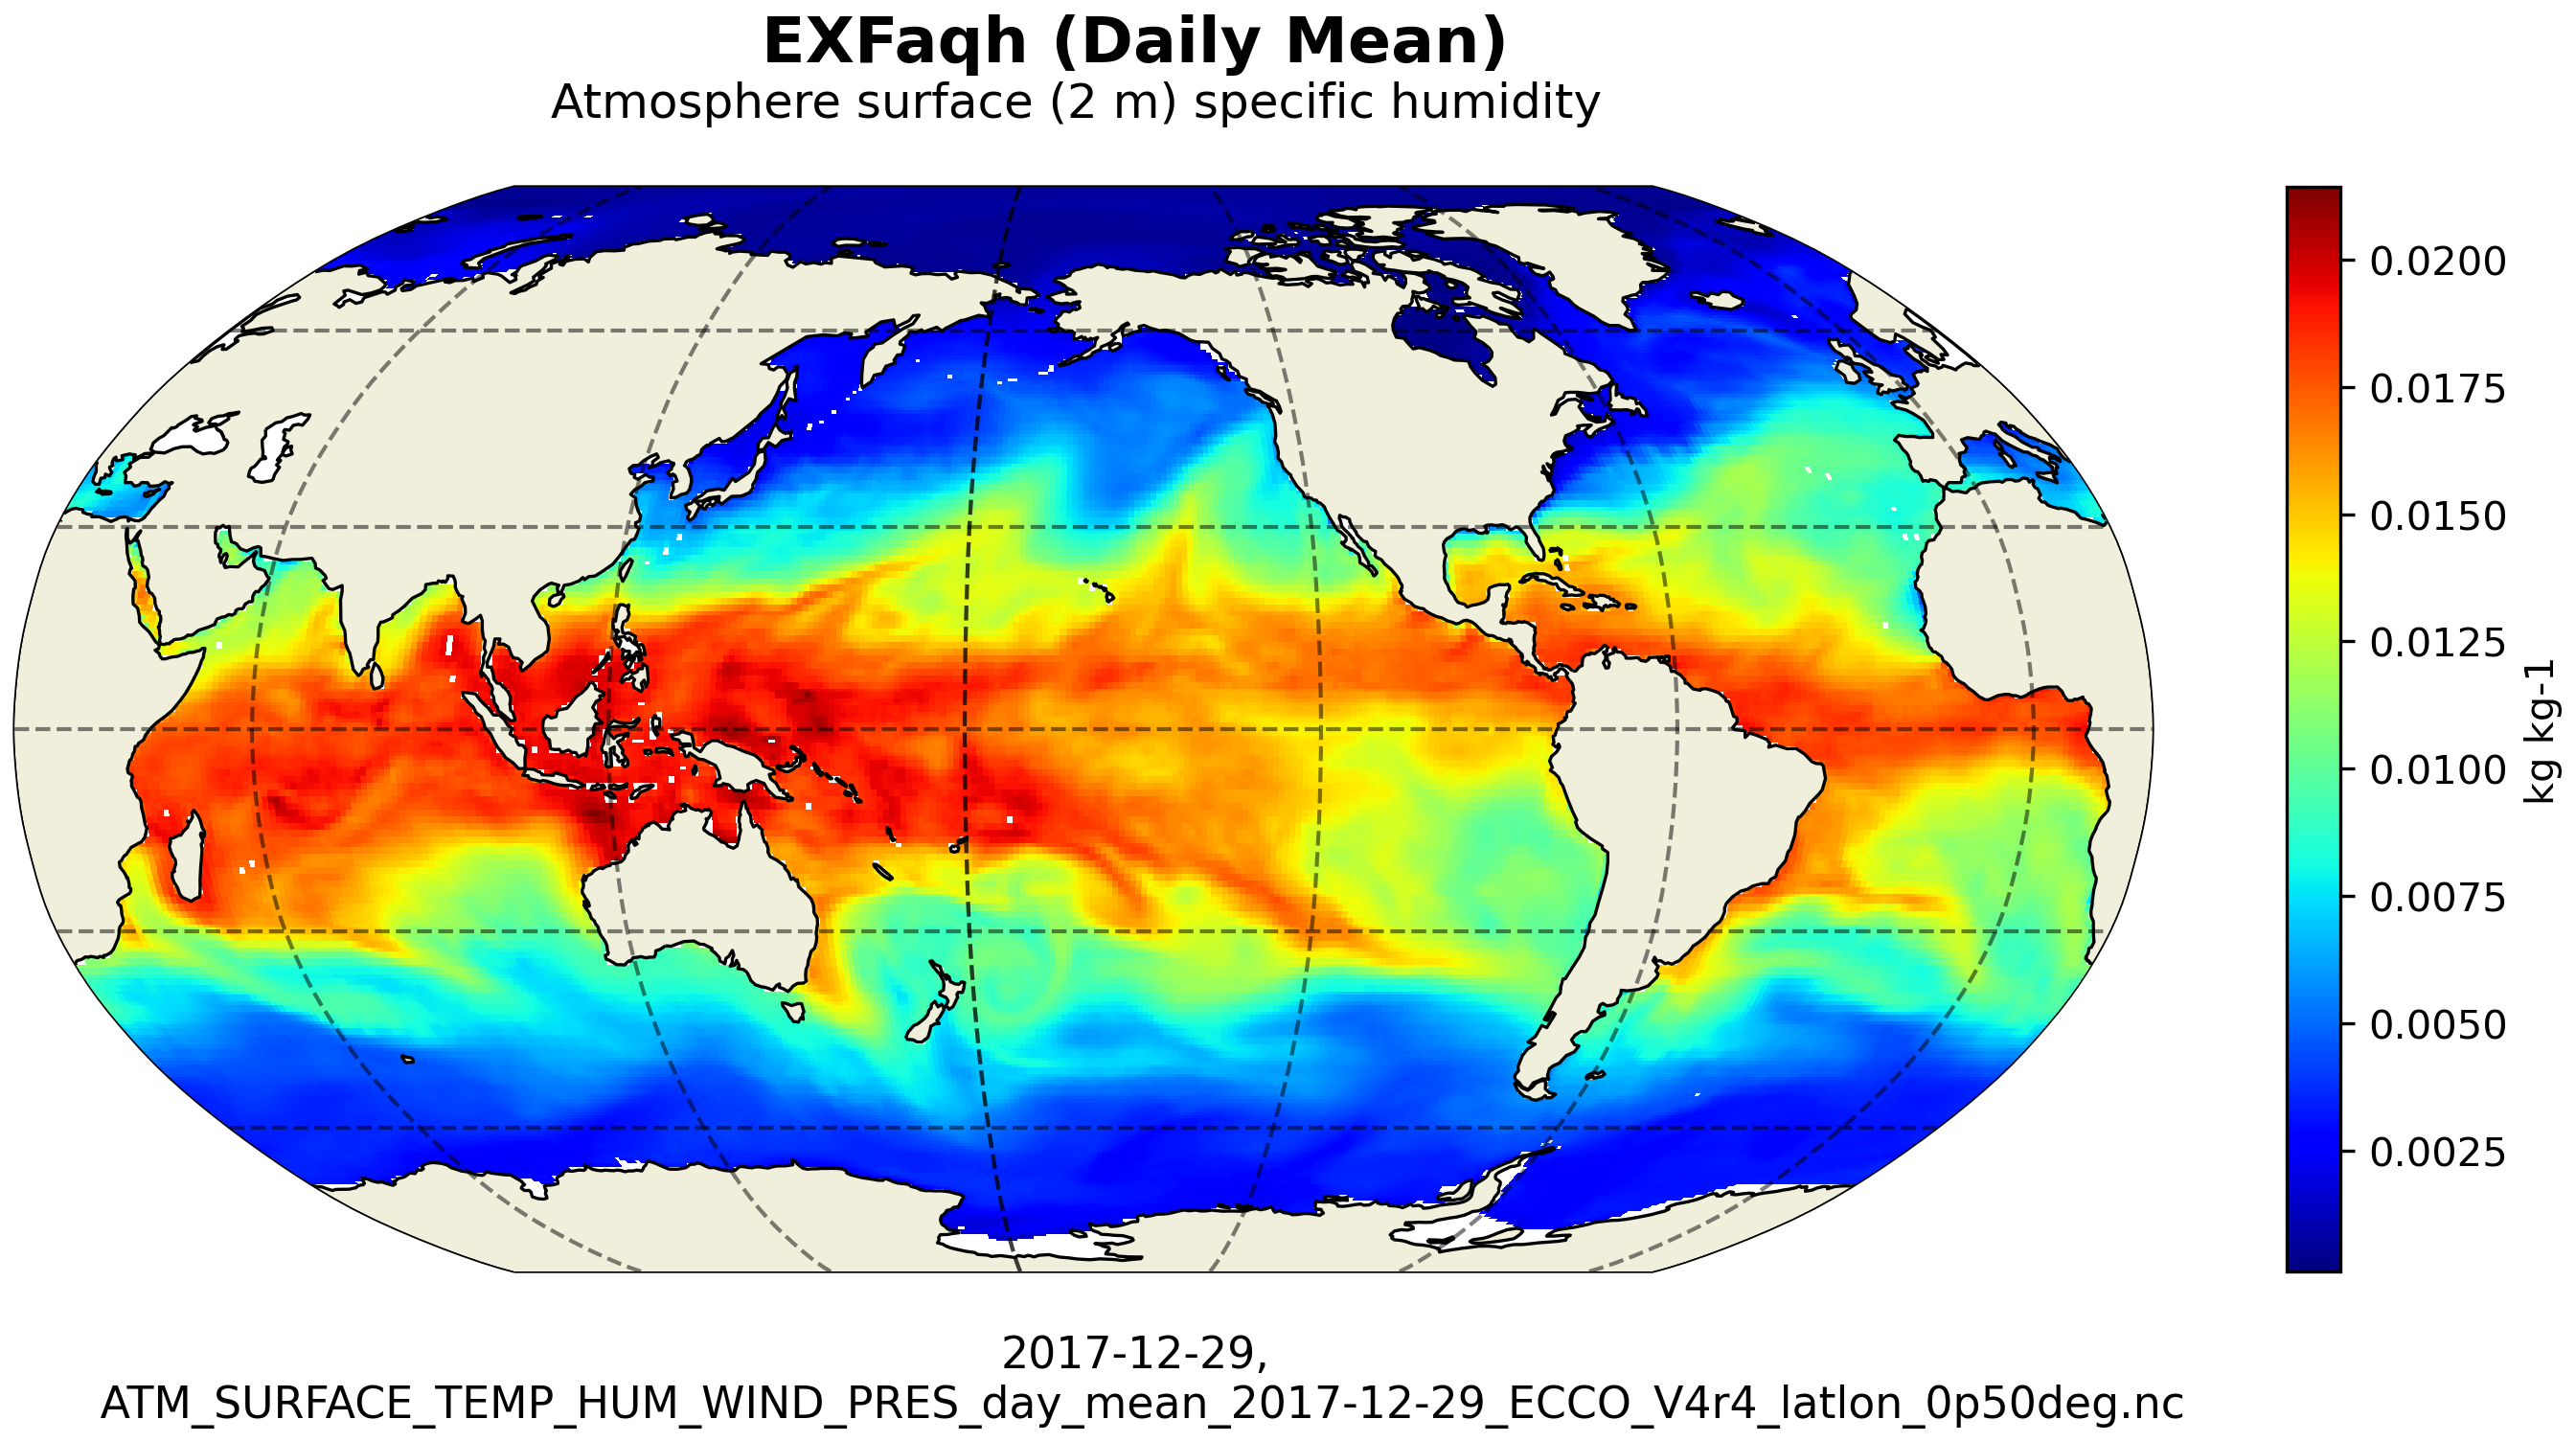
\includegraphics[width=\textwidth]{../images/plots/latlon_plots/Atmosphere_Surface_Temperature_Humidity_Wind_and_Pressure/EXFaqh.png}
\caption{Dataset: ATM\_SURFACE\_TEMP\_HUM\_WIND\_PRES Variable: EXFaqh}
\label{tab:table-ATM_SURFACE_TEMP_HUM_WIND_PRES_EXFaqh-Plot}
\end{figure}
\pagebreak
\subsubsection{Latlon Variable EXFatemp}
\begin{longtable}{|p{0.06\textwidth}|p{0.41\textwidth}|p{0.39\textwidth}|p{0.06\textwidth}|}
\caption{CDL description of ATM\_SURFACE\_TEMP\_HUM\_WIND\_PRES's EXFatemp variable}
\label{tab:table-ATM_SURFACE_TEMP_HUM_WIND_PRES_EXFatemp} \\ 
\hline \endhead \hline \endfoot
\rowcolor{lightgray} \textbf{Storage Type} & \textbf{Variable Name} & \textbf{Description} & \textbf{Unit} \\ \hline
float32 & EXFatemp & Atmosphere surface (2 m) air temperature  & degree\_K \\ \hline
\rowcolor{lightgray}  \multicolumn{4}{|p{1.00\textwidth}|}{\textbf{CDL Description}} \\ \hline
\multicolumn{4}{|p{1.00\textwidth}|}{\makecell{\parbox{1\textwidth}{float32 EXFatemp(time, latitude, longitude)\\
\hspace*{0.5cm}EXFatemp: \_FillValue = 9.96921e+36\\
\hspace*{0.5cm}EXFatemp: coverage\_content\_type = modelResult\\
\hspace*{0.5cm}EXFatemp: long\_name = Atmosphere surface (2 m) air temperature \\
\hspace*{0.5cm}EXFatemp: standard\_name = air\_temperature\\
\hspace*{0.5cm}EXFatemp: units = degree\_K\\
\hspace*{0.5cm}EXFatemp: coordinates = time\\
\hspace*{0.5cm}EXFatemp: valid\_min = 195.37054443359375\\
\hspace*{0.5cm}EXFatemp: valid\_max = 312.8451232910156}}} \\ \hline
\rowcolor{lightgray} \multicolumn{4}{|p{1.00\textwidth}|}{\textbf{Comments}} \\ \hline
\multicolumn{4}{|p{1\textwidth}|}{Surface (2 m) air temperature over open water. Note: sum of ERA-Interim surface air temperature and the control adjustment from ocean state estimation.} \\ \hline
\end{longtable}

\begin{figure}[H]
\centering
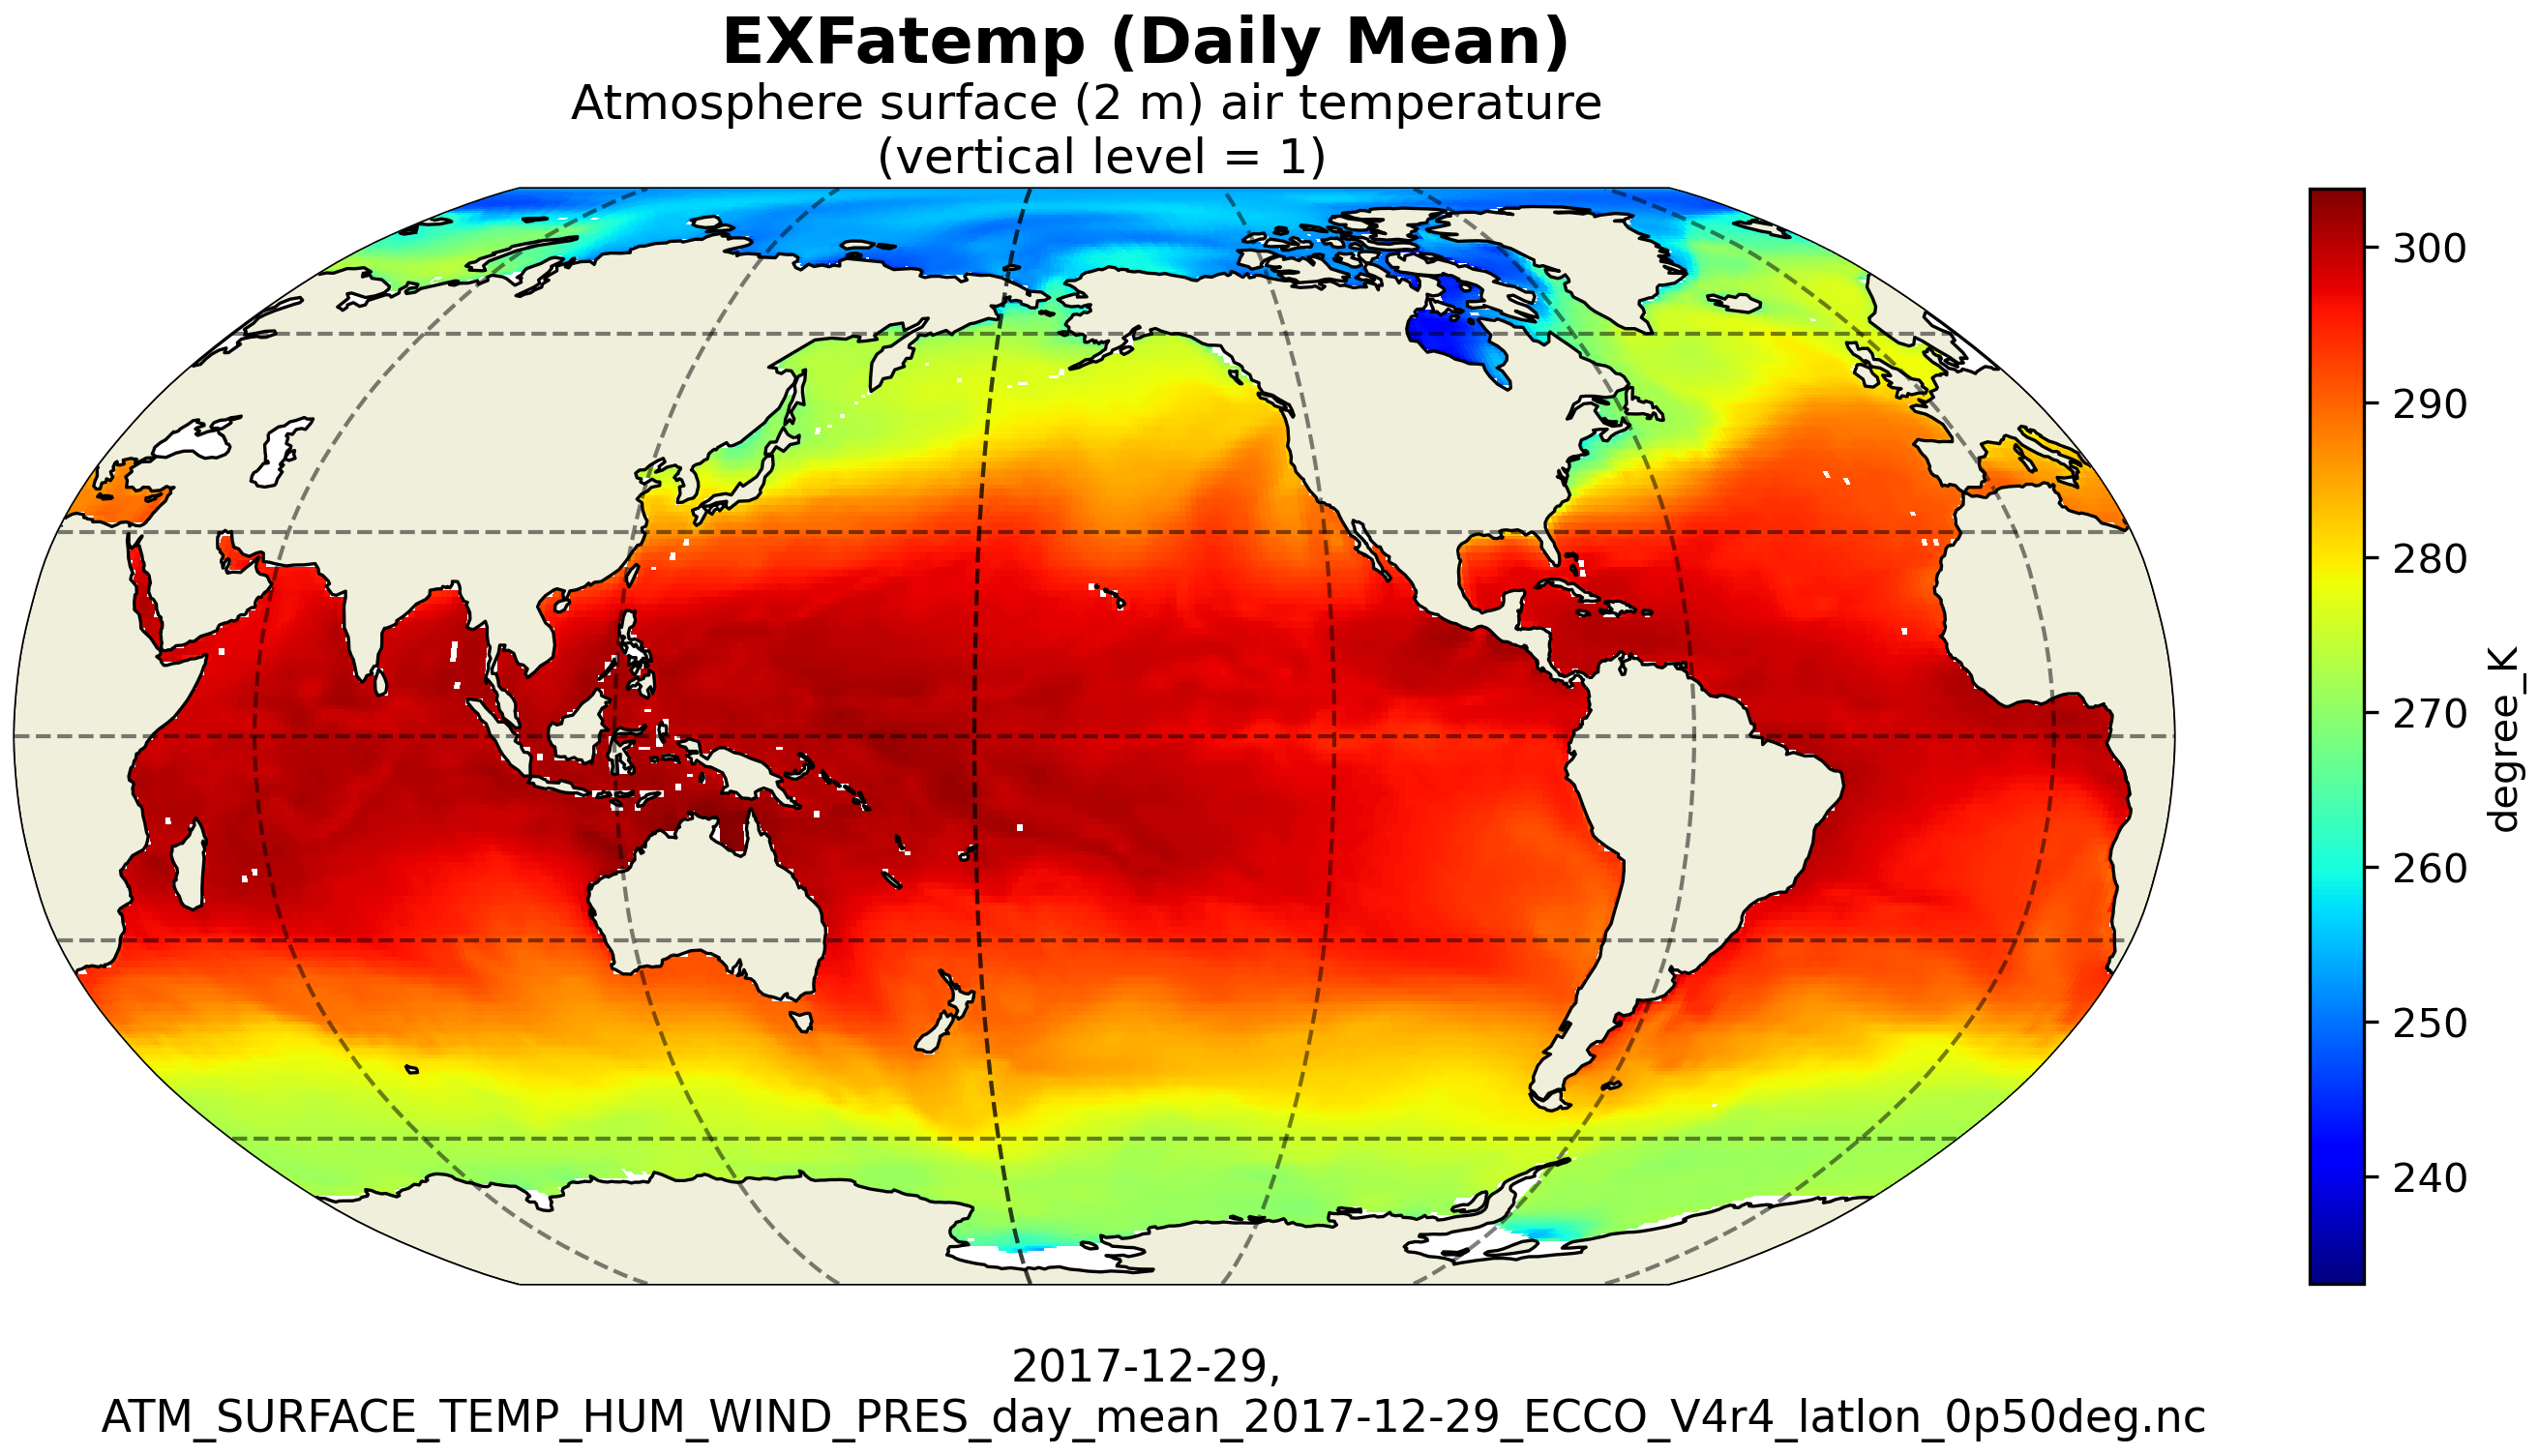
\includegraphics[width=\textwidth]{../images/plots/latlon_plots/Atmosphere_Surface_Temperature_Humidity_Wind_and_Pressure/EXFatemp.png}
\caption{Dataset: ATM\_SURFACE\_TEMP\_HUM\_WIND\_PRES Variable: EXFatemp}
\label{tab:table-ATM_SURFACE_TEMP_HUM_WIND_PRES_EXFatemp-Plot}
\end{figure}
\pagebreak
\subsubsection{Latlon Variable EXFewind}
\begin{longtable}{|p{0.06\textwidth}|p{0.41\textwidth}|p{0.39\textwidth}|p{0.06\textwidth}|}
\caption{CDL description of ATM\_SURFACE\_TEMP\_HUM\_WIND\_PRES's EXFewind variable}
\label{tab:table-ATM_SURFACE_TEMP_HUM_WIND_PRES_EXFewind} \\ 
\hline \endhead \hline \endfoot
\rowcolor{lightgray} \textbf{Storage Type} & \textbf{Variable Name} & \textbf{Description} & \textbf{Unit} \\ \hline
float32 & EXFewind & Zonal (east-west) wind speed & m s-1 \\ \hline
\rowcolor{lightgray}  \multicolumn{4}{|p{1.00\textwidth}|}{\textbf{CDL Description}} \\ \hline
\multicolumn{4}{|p{1.00\textwidth}|}{\makecell{\parbox{1\textwidth}{float32 EXFewind(time, latitude, longitude)\\
\hspace*{0.5cm}EXFewind: \_FillValue = 9.96921e+36\\
\hspace*{0.5cm}EXFewind: coverage\_content\_type = modelResult\\
\hspace*{0.5cm}EXFewind: long\_name = Zonal (east: west) wind speed\\
\hspace*{0.5cm}EXFewind: standard\_name = eastward\_wind\\
\hspace*{0.5cm}EXFewind: units = m s: 1\\
\hspace*{0.5cm}EXFewind: coordinates = time\\
\hspace*{0.5cm}EXFewind: valid\_min = : 33.524742126464844\\
\hspace*{0.5cm}EXFewind: valid\_max = 39.48556900024414}}} \\ \hline
\rowcolor{lightgray} \multicolumn{4}{|p{1.00\textwidth}|}{\textbf{Comments}} \\ \hline
\multicolumn{4}{|p{1\textwidth}|}{Zonal (east-west) component of ocean surface wind. Note: EXFewind is calculated by interpolating the model's x and y components of wind velocity (EXFuwind and EXFvwind) to tracer cell centers and then finding the zonal component of the interpolated vectors. ECCO V4r4 is forced with wind stress (see EXFtaux, EXFtauy), not vector winds + bulk formulae. EXFewind is calculated by converting wind stress to vector wind using bulk formulae.} \\ \hline
\end{longtable}

\begin{figure}[H]
\centering
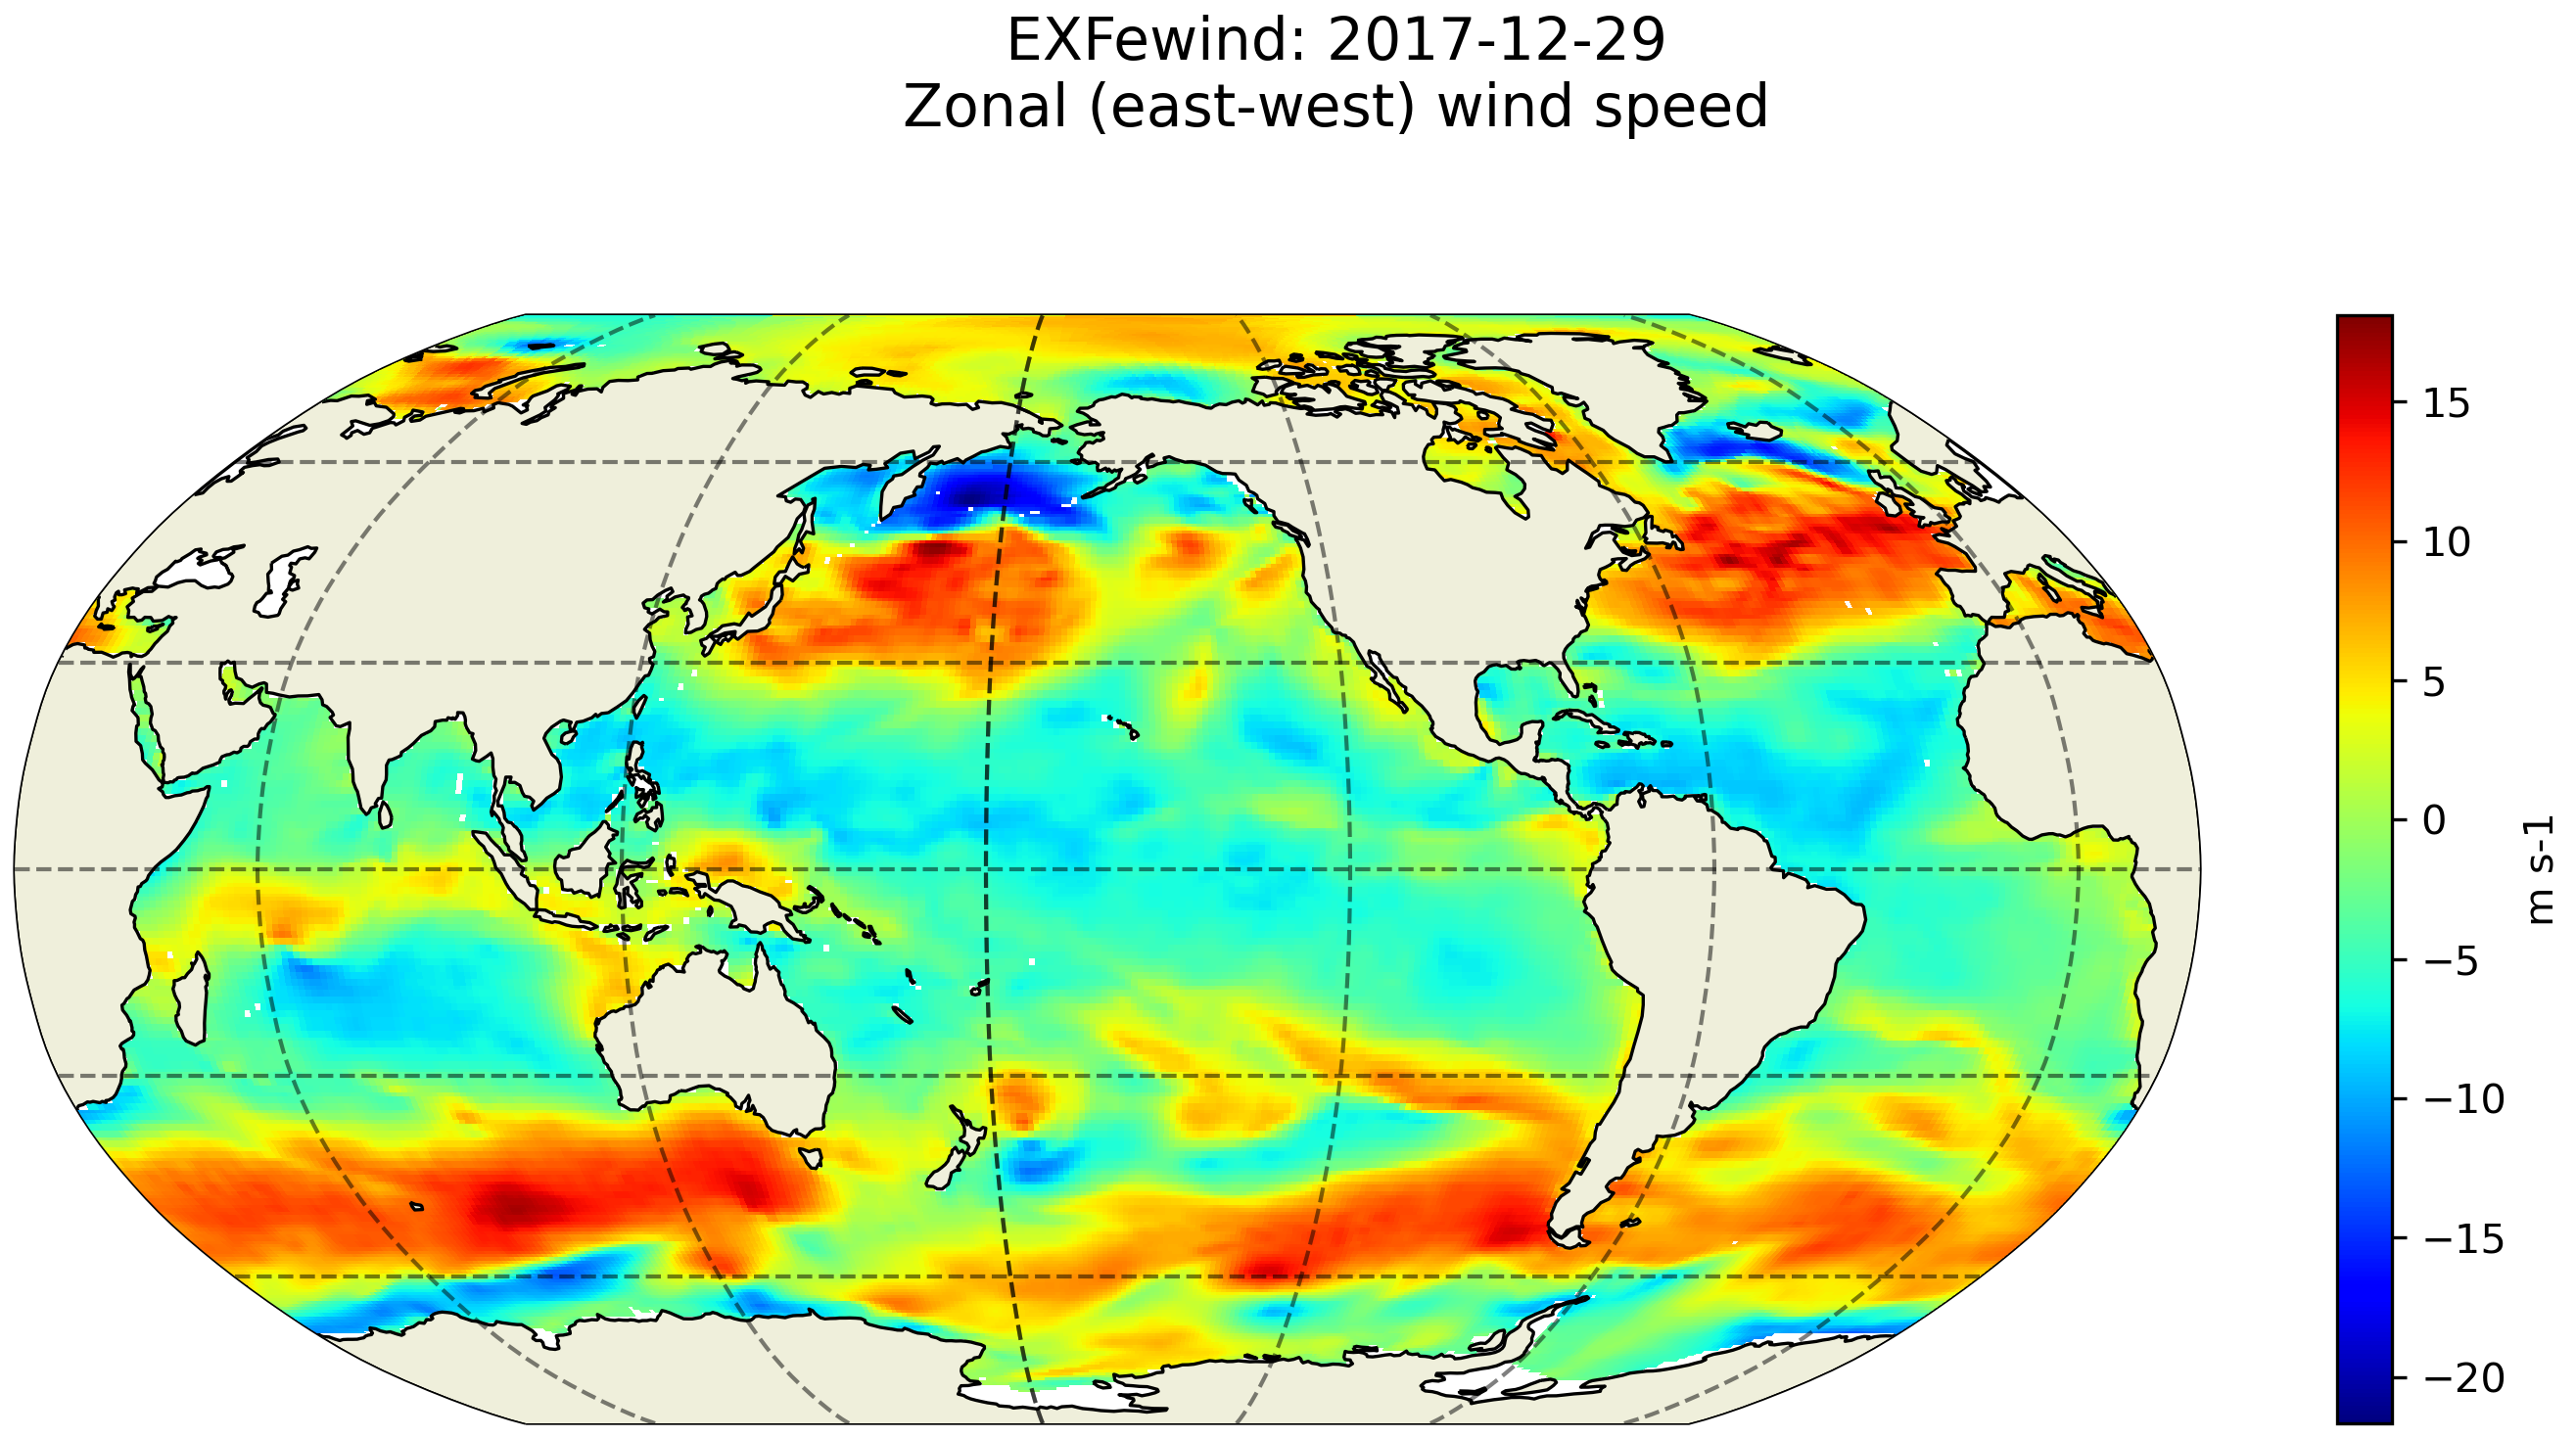
\includegraphics[width=\textwidth]{../images/plots/latlon_plots/Atmosphere_Surface_Temperature_Humidity_Wind_and_Pressure/EXFewind.png}
\caption{Dataset: ATM\_SURFACE\_TEMP\_HUM\_WIND\_PRES Variable: EXFewind}
\label{tab:table-ATM_SURFACE_TEMP_HUM_WIND_PRES_EXFewind-Plot}
\end{figure}
\pagebreak
\subsubsection{Latlon Variable EXFnwind}
\begin{longtable}{|p{0.06\textwidth}|p{0.41\textwidth}|p{0.39\textwidth}|p{0.06\textwidth}|}
\caption{CDL description of ATM\_SURFACE\_TEMP\_HUM\_WIND\_PRES's EXFnwind variable}
\label{tab:table-ATM_SURFACE_TEMP_HUM_WIND_PRES_EXFnwind} \\ 
\hline \endhead \hline \endfoot
\rowcolor{lightgray} \textbf{Storage Type} & \textbf{Variable Name} & \textbf{Description} & \textbf{Unit} \\ \hline
float32 & EXFnwind & Meridional (north-south) wind speed & m s-1 \\ \hline
\rowcolor{lightgray}  \multicolumn{4}{|p{1.00\textwidth}|}{\textbf{CDL Description}} \\ \hline
\multicolumn{4}{|p{1.00\textwidth}|}{\makecell{\parbox{1\textwidth}{float32 EXFnwind(time, latitude, longitude)\\
\hspace*{0.5cm}EXFnwind: \_FillValue = 9.96921e+36\\
\hspace*{0.5cm}EXFnwind: coverage\_content\_type = modelResult\\
\hspace*{0.5cm}EXFnwind: long\_name = Meridional (north: south) wind speed\\
\hspace*{0.5cm}EXFnwind: standard\_name = northward\_wind\\
\hspace*{0.5cm}EXFnwind: units = m s: 1\\
\hspace*{0.5cm}EXFnwind: coordinates = time\\
\hspace*{0.5cm}EXFnwind: valid\_min = : 30.042686462402344\\
\hspace*{0.5cm}EXFnwind: valid\_max = 33.95014190673828}}} \\ \hline
\rowcolor{lightgray} \multicolumn{4}{|p{1.00\textwidth}|}{\textbf{Comments}} \\ \hline
\multicolumn{4}{|p{1\textwidth}|}{Meridional (north-south) component of ocean surface wind. Note: EXFnwind is calculated by interpolating the model's x and y components of wind velocity (EXFuwind and EXFvwind) to tracer cell centers and then finding the meridional component of the interpolated vectors. ECCO V4r4 is forced with wind stress (see EXFtaux, EXFtauy), not vector winds + bulk formulae.  EXFnwind is calculated by converting wind stress to vector wind using bulk formulae.} \\ \hline
\end{longtable}

\begin{figure}[H]
\centering
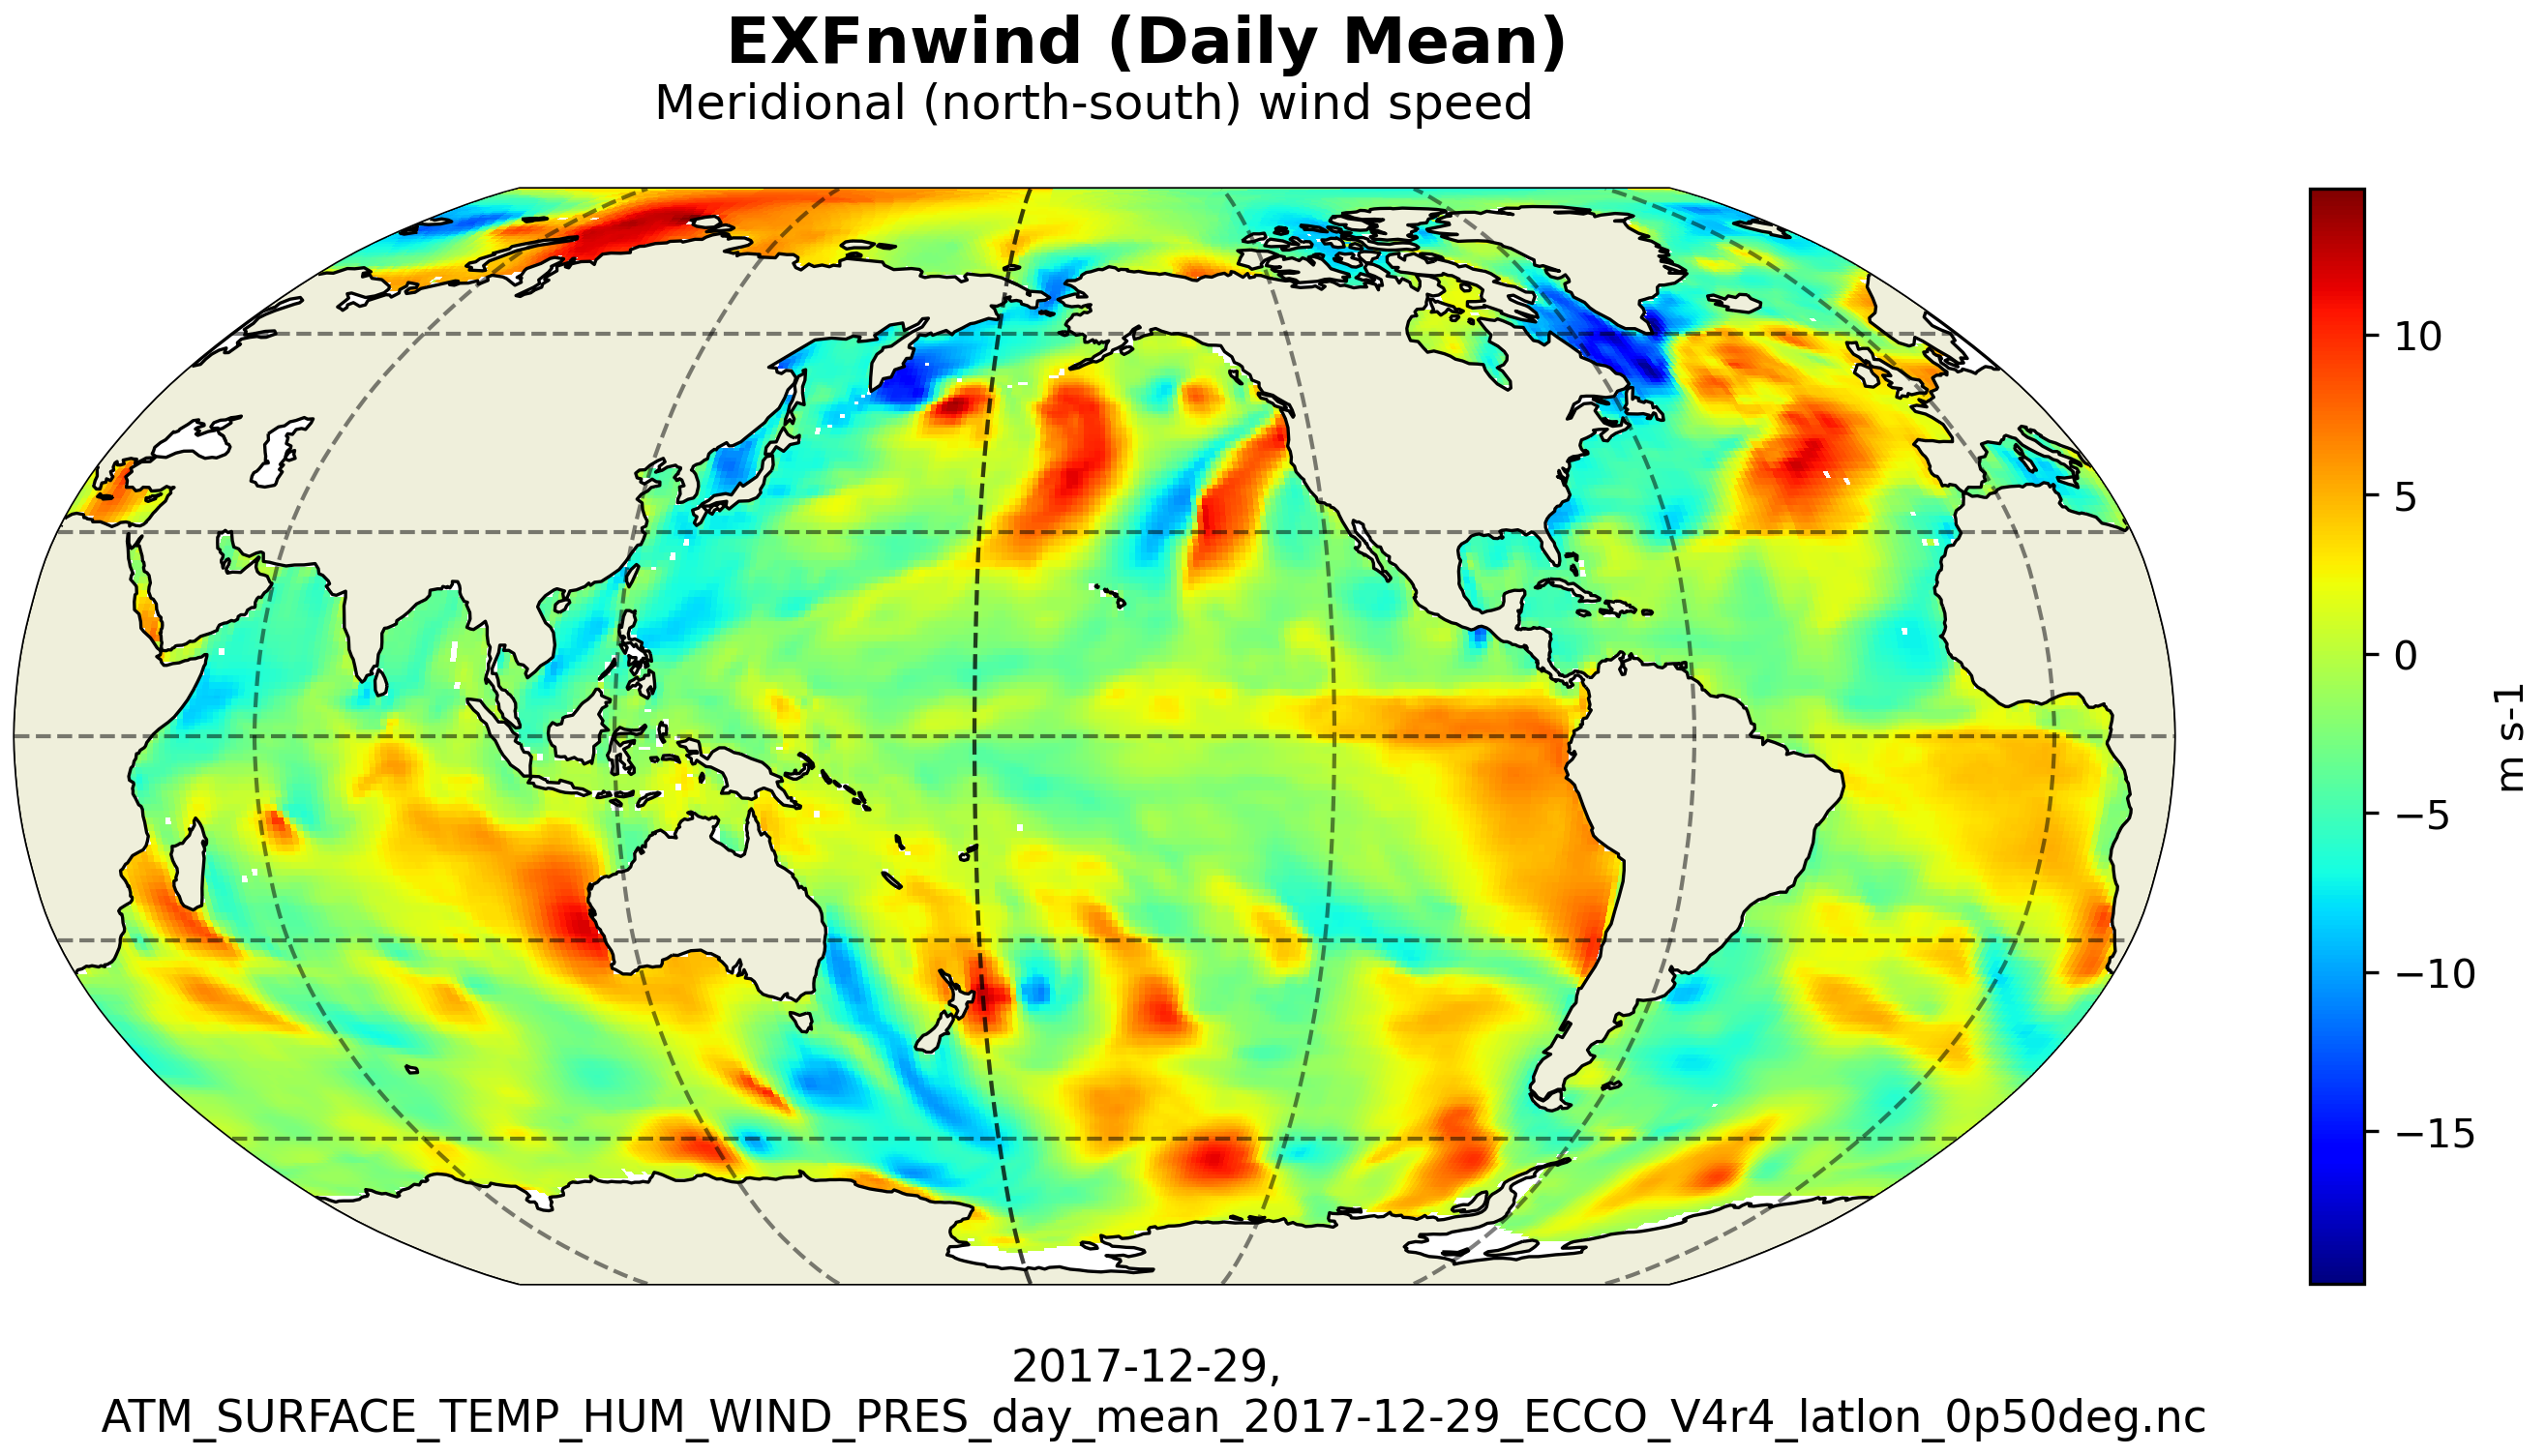
\includegraphics[width=\textwidth]{../images/plots/latlon_plots/Atmosphere_Surface_Temperature_Humidity_Wind_and_Pressure/EXFnwind.png}
\caption{Dataset: ATM\_SURFACE\_TEMP\_HUM\_WIND\_PRES Variable: EXFnwind}
\label{tab:table-ATM_SURFACE_TEMP_HUM_WIND_PRES_EXFnwind-Plot}
\end{figure}
\pagebreak
\subsubsection{Latlon Variable EXFpress}
\begin{longtable}{|p{0.06\textwidth}|p{0.41\textwidth}|p{0.39\textwidth}|p{0.06\textwidth}|}
\caption{CDL description of ATM\_SURFACE\_TEMP\_HUM\_WIND\_PRES's EXFpress variable}
\label{tab:table-ATM_SURFACE_TEMP_HUM_WIND_PRES_EXFpress} \\ 
\hline \endhead \hline \endfoot
\rowcolor{lightgray} \textbf{Storage Type} & \textbf{Variable Name} & \textbf{Description} & \textbf{Unit} \\ \hline
float32 & EXFpress & Atmosphere surface pressure & N m-2 \\ \hline
\rowcolor{lightgray}  \multicolumn{4}{|p{1.00\textwidth}|}{\textbf{CDL Description}} \\ \hline
\multicolumn{4}{|p{1.00\textwidth}|}{\makecell{\parbox{1\textwidth}{float32 EXFpress(time, latitude, longitude)\\
\hspace*{0.5cm}EXFpress: \_FillValue = 9.96921e+36\\
\hspace*{0.5cm}EXFpress: coverage\_content\_type = modelResult\\
\hspace*{0.5cm}EXFpress: long\_name = Atmosphere surface pressure\\
\hspace*{0.5cm}EXFpress: standard\_name = surface\_air\_pressure\\
\hspace*{0.5cm}EXFpress: units = N m: 2\\
\hspace*{0.5cm}EXFpress: coordinates = time\\
\hspace*{0.5cm}EXFpress: valid\_min = 92090.3125\\
\hspace*{0.5cm}EXFpress: valid\_max = 106314.7734375}}} \\ \hline
\rowcolor{lightgray} \multicolumn{4}{|p{1.00\textwidth}|}{\textbf{Comments}} \\ \hline
\multicolumn{4}{|p{1\textwidth}|}{Atmospheric pressure field at sea level. Note: ERA-Interim atmospheric pressure, with air tides removed using a variety of methods. Not adjusted by the ocean state estimation.} \\ \hline
\end{longtable}

\begin{figure}[H]
\centering
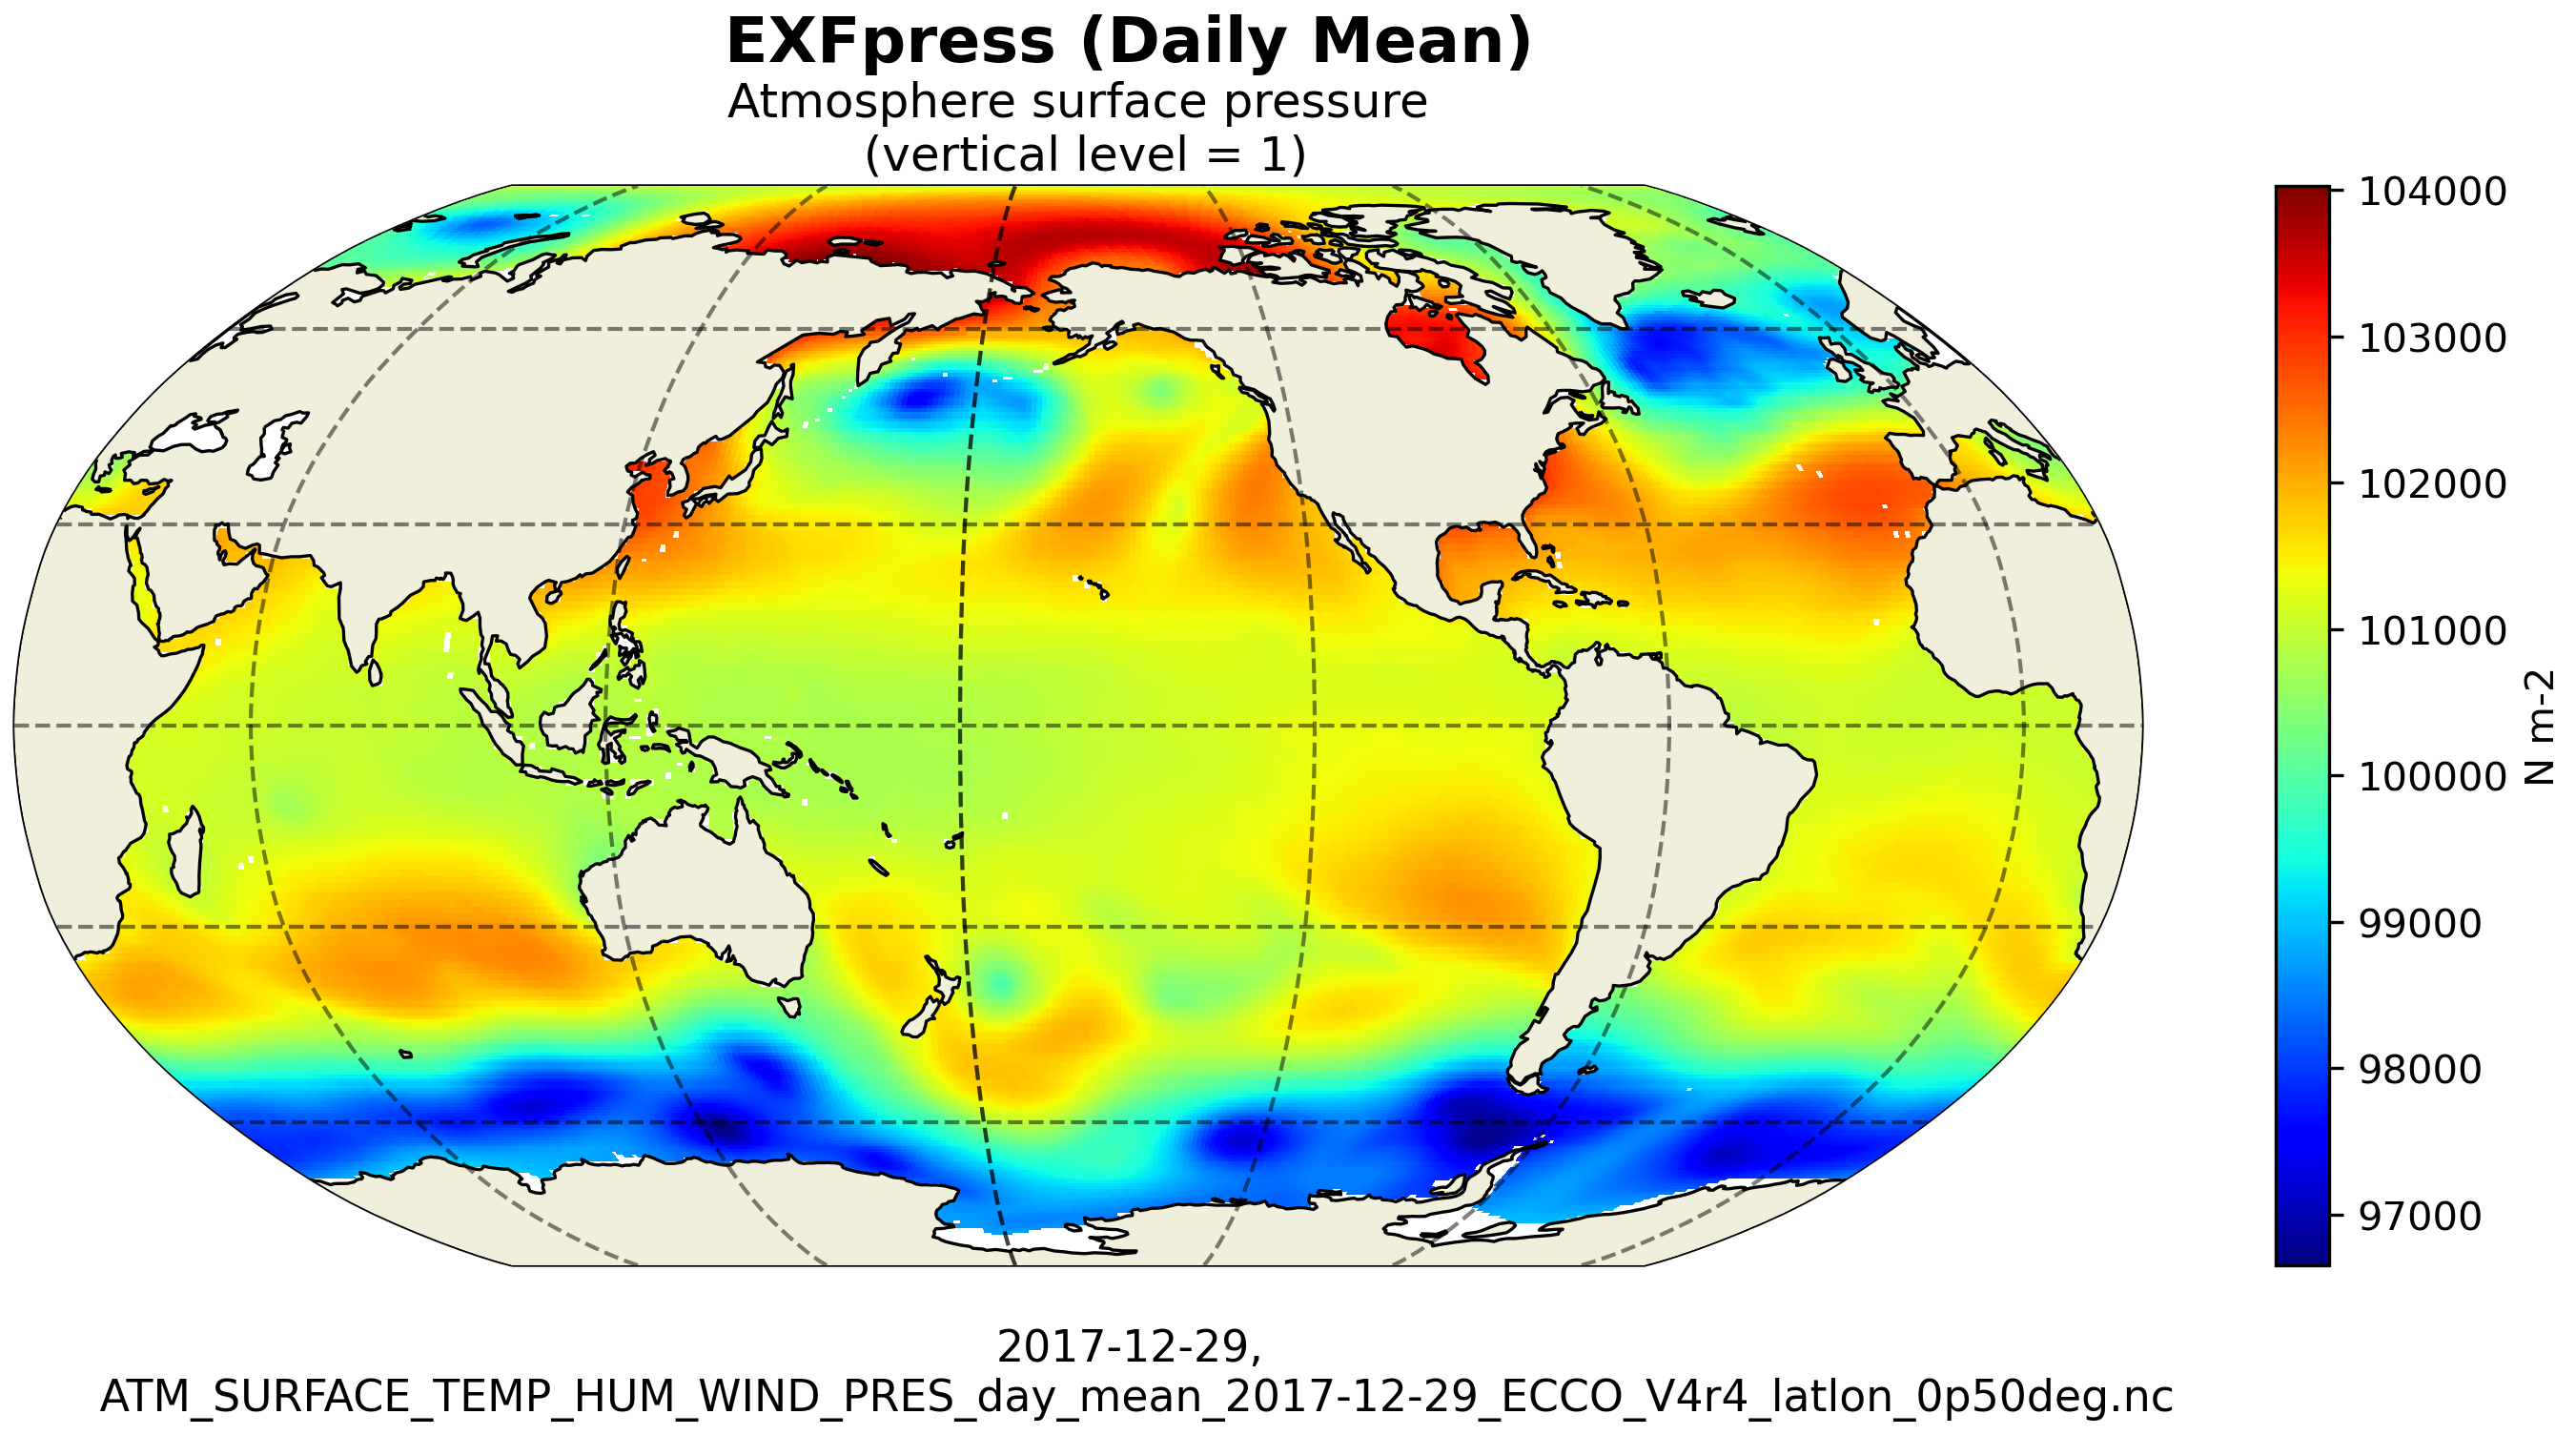
\includegraphics[width=\textwidth]{../images/plots/latlon_plots/Atmosphere_Surface_Temperature_Humidity_Wind_and_Pressure/EXFpress.png}
\caption{Dataset: ATM\_SURFACE\_TEMP\_HUM\_WIND\_PRES Variable: EXFpress}
\label{tab:table-ATM_SURFACE_TEMP_HUM_WIND_PRES_EXFpress-Plot}
\end{figure}
\pagebreak
\subsubsection{Latlon Variable EXFwspee}
\begin{longtable}{|p{0.06\textwidth}|p{0.41\textwidth}|p{0.39\textwidth}|p{0.06\textwidth}|}
\caption{CDL description of ATM\_SURFACE\_TEMP\_HUM\_WIND\_PRES's EXFwspee variable}
\label{tab:table-ATM_SURFACE_TEMP_HUM_WIND_PRES_EXFwspee} \\ 
\hline \endhead \hline \endfoot
\rowcolor{lightgray} \textbf{Storage Type} & \textbf{Variable Name} & \textbf{Description} & \textbf{Unit} \\ \hline
float32 & EXFwspee & Wind speed & m s-1 \\ \hline
\rowcolor{lightgray}  \multicolumn{4}{|p{1.00\textwidth}|}{\textbf{CDL Description}} \\ \hline
\multicolumn{4}{|p{1.00\textwidth}|}{\makecell{\parbox{1\textwidth}{float32 EXFwspee(time, latitude, longitude)\\
\hspace*{0.5cm}EXFwspee: \_FillValue = 9.96921e+36\\
\hspace*{0.5cm}EXFwspee: coverage\_content\_type = modelResult\\
\hspace*{0.5cm}EXFwspee: long\_name = Wind speed\\
\hspace*{0.5cm}EXFwspee: standard\_name = wind\_speed\\
\hspace*{0.5cm}EXFwspee: units = m s: 1\\
\hspace*{0.5cm}EXFwspee: coordinates = time\\
\hspace*{0.5cm}EXFwspee: valid\_min = 0.27271032333374023\\
\hspace*{0.5cm}EXFwspee: valid\_max = 45.87086486816406}}} \\ \hline
\rowcolor{lightgray} \multicolumn{4}{|p{1.00\textwidth}|}{\textbf{Comments}} \\ \hline
\multicolumn{4}{|p{1\textwidth}|}{10-m wind speed magnitude (>= 0 ) over open water. Only used for the calculation of air-sea fluxes using bulk formulae. Note: not adjusted by the ocean state estimation and not necesarily consistent with EXFuwind and EXFvwind because EXFuwind and EXFvwind are calculated from EXFtaux and EXFtauy using bulk formulae. EXFwspee != sqrt(EXFuwind**2 + EXFvwind**2.} \\ \hline
\end{longtable}

\begin{figure}[H]
\centering
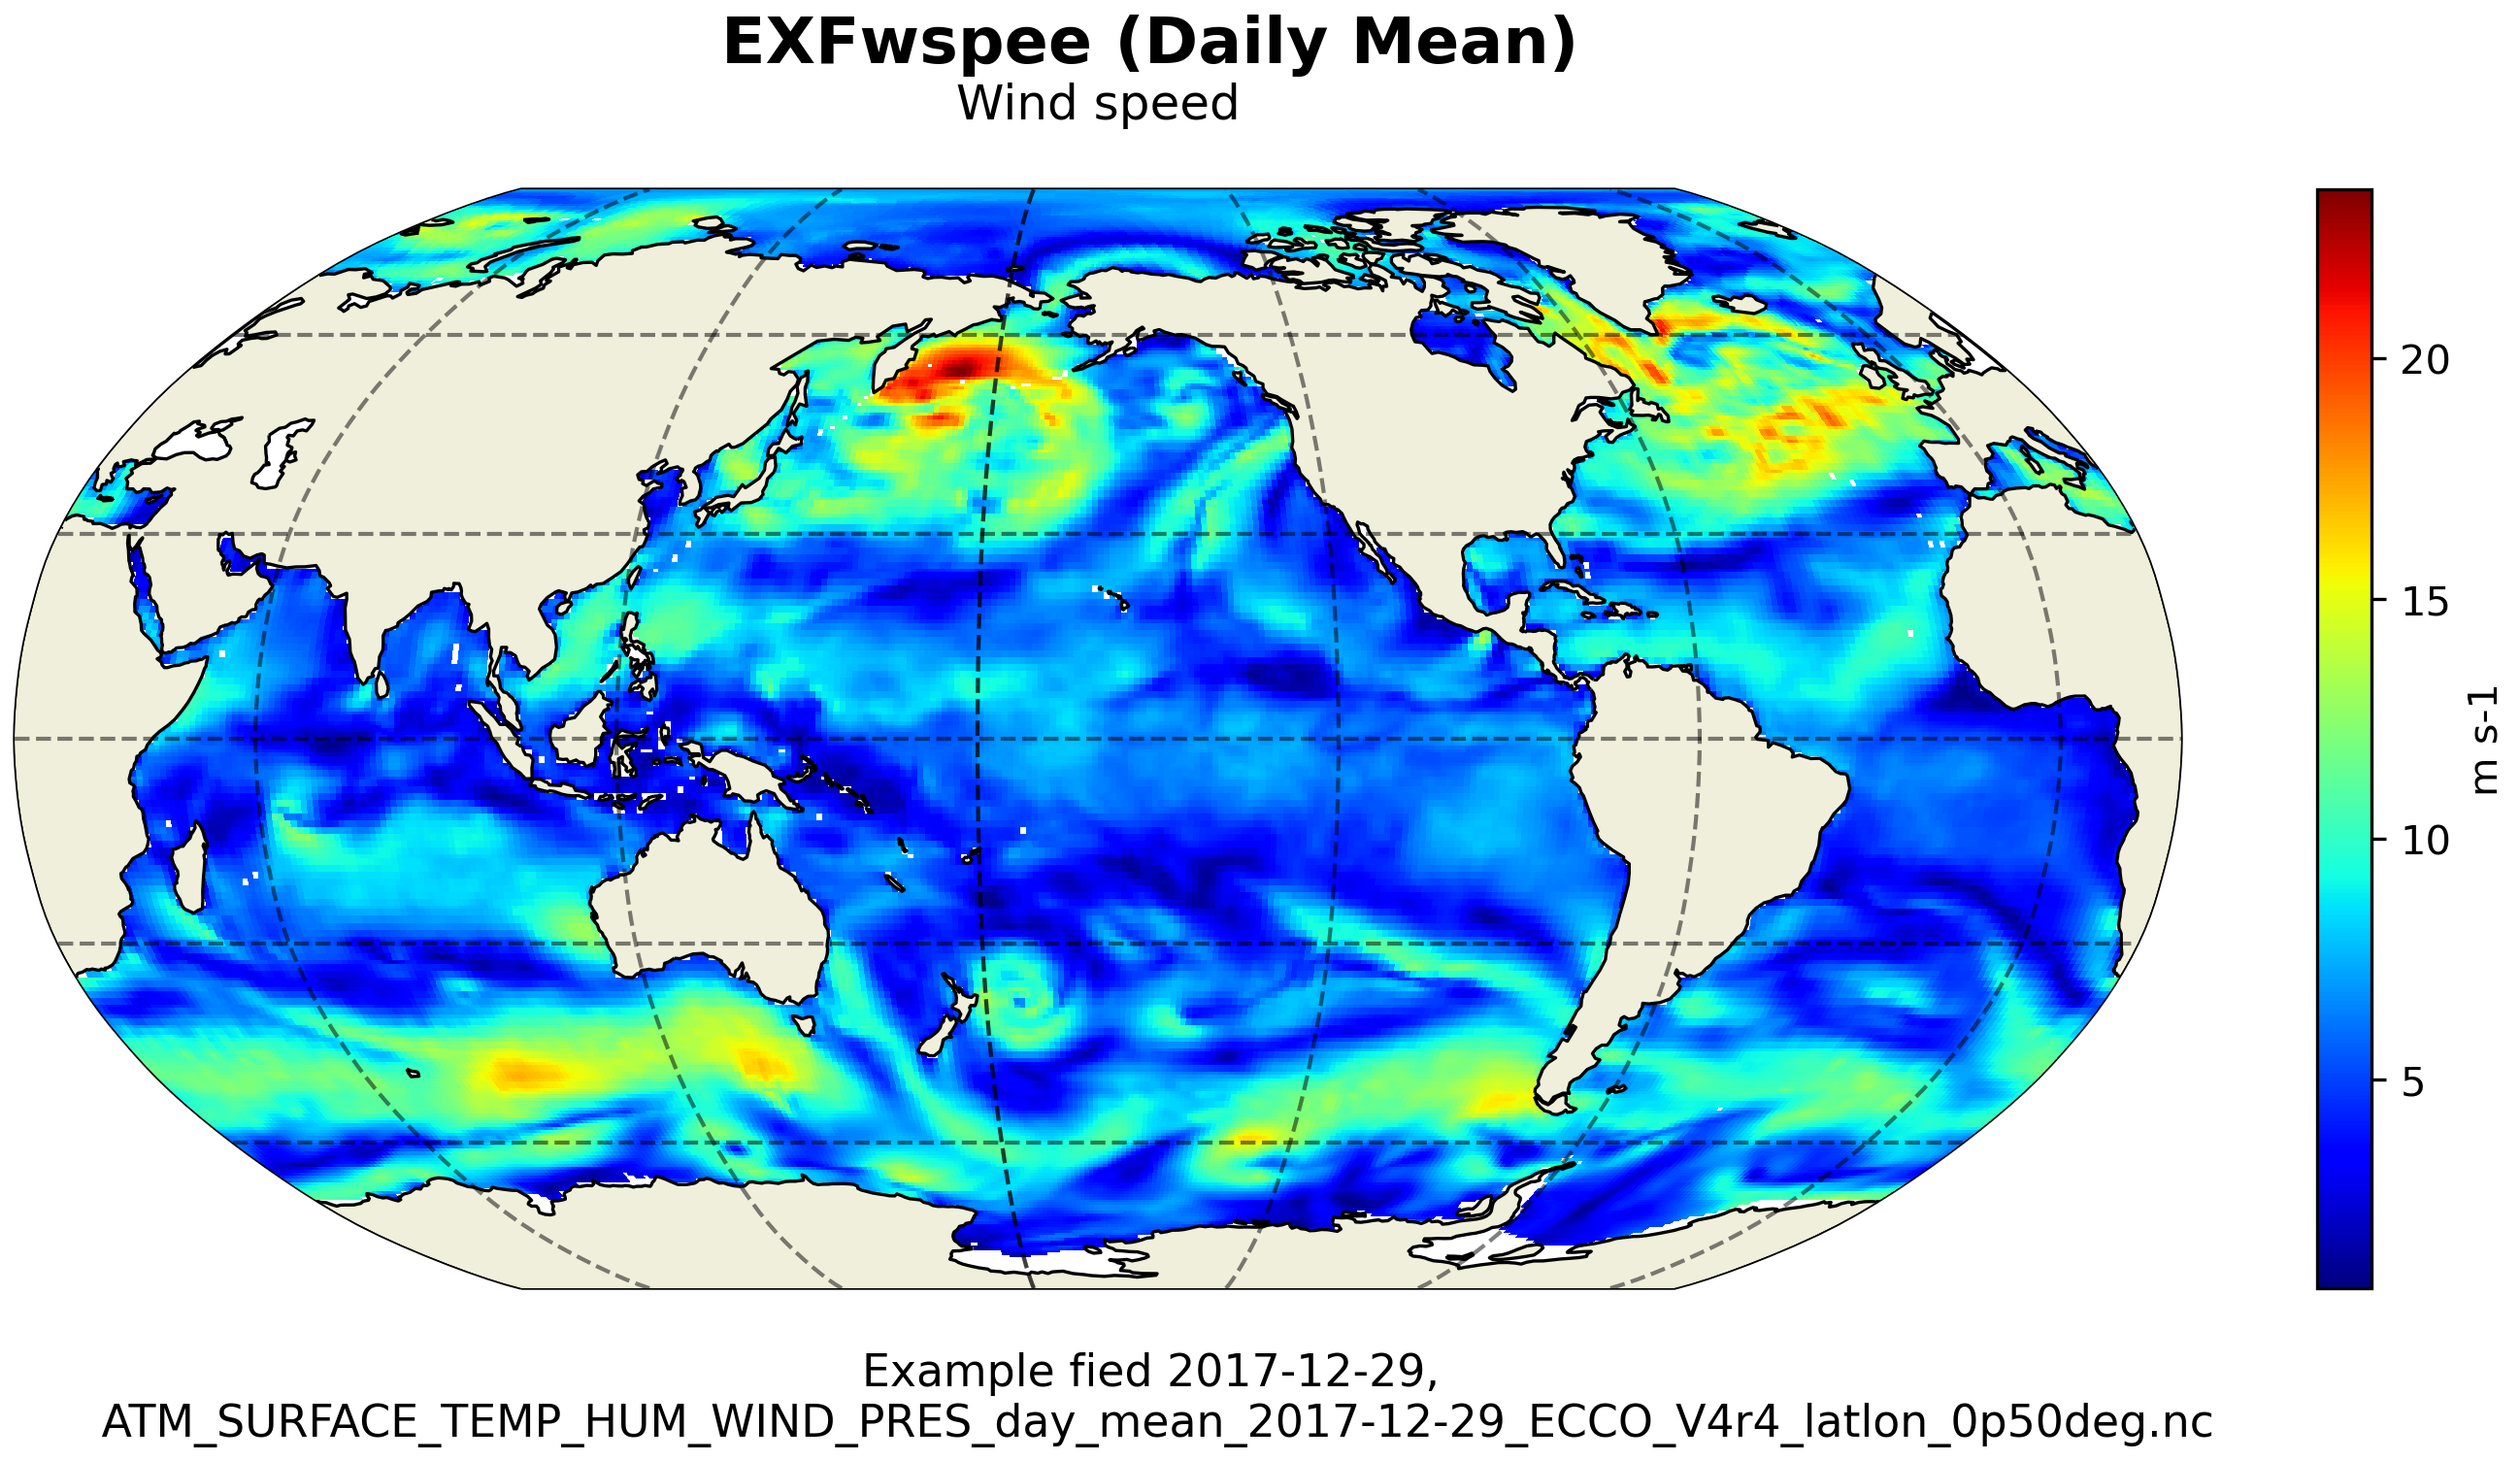
\includegraphics[width=\textwidth]{../images/plots/latlon_plots/Atmosphere_Surface_Temperature_Humidity_Wind_and_Pressure/EXFwspee.png}
\caption{Dataset: ATM\_SURFACE\_TEMP\_HUM\_WIND\_PRES Variable: EXFwspee}
\label{tab:table-ATM_SURFACE_TEMP_HUM_WIND_PRES_EXFwspee-Plot}
\end{figure}
\pagebreak
\subsection{Latlon NetCDF OCEAN\_AND\_ICE\_SURFACE\_FW\_FLUX}
\newp
\begin{longtable}{|p{0.1\textwidth}|p{0.5\textwidth}|}
\caption{Variables in the dataset OCEAN\_AND\_ICE\_SURFACE\_FW\_FLUX}
\label{tab:table-OCEAN_AND_ICE_SURFACE_FW_FLUX-fields} \\ 
\hline \endhead \hline \endfoot
\rowcolor{lightgray} \textbf{Dataset:} & \textbf{OCEAN\_AND\_ICE\_SURFACE\_FW\_FLUX} \\ \hline
Field: &EXFpreci \\ \hline
Field: &EXFevap \\ \hline
Field: &EXFroff \\ \hline
Field: &SIsnPrcp \\ \hline
Field: &EXFempmr \\ \hline
Field: &oceFWflx \\ \hline
Field: &SIatmFW \\ \hline
Field: &SFLUX \\ \hline
Field: &SIacSubl \\ \hline
Field: &SIrsSubl \\ \hline
Field: &SIfwThru \\ \hline
\end{longtable}

\pagebreak
\subsubsection{Latlon Variable EXFempmr}
\begin{longtable}{|p{0.06\textwidth}|p{0.41\textwidth}|p{0.39\textwidth}|p{0.06\textwidth}|}
\caption{CDL description of OCEAN\_AND\_ICE\_SURFACE\_FW\_FLUX's EXFempmr variable}
\label{tab:table-OCEAN_AND_ICE_SURFACE_FW_FLUX_EXFempmr} \\ 
\hline \endhead \hline \endfoot
\rowcolor{lightgray} \textbf{Storage Type} & \textbf{Variable Name} & \textbf{Description} & \textbf{Unit} \\ \hline
float32 & EXFempmr & Open ocean net surface freshwater flux from precipitation, evaporation, and runoff & m s-1 \\ \hline
\rowcolor{lightgray}  \multicolumn{4}{|p{1.00\textwidth}|}{\textbf{CDL Description}} \\ \hline
\multicolumn{4}{|p{1.00\textwidth}|}{\makecell{\parbox{1\textwidth}{float32 EXFempmr(time, latitude, longitude)\\
\hspace*{0.5cm}EXFempmr: \_FillValue = 9.96921e+36\\
\hspace*{0.5cm}EXFempmr: coverage\_content\_type = modelResult\\
\hspace*{0.5cm}EXFempmr: direction = >0 increases salinity (SALT)\\
\hspace*{0.5cm}EXFempmr: long\_name = Open ocean net surface freshwater flux from precipitation\\
evaporation\\
and runoff\\
\hspace*{0.5cm}EXFempmr: units = m s: 1\\
\hspace*{0.5cm}EXFempmr: coordinates = time\\
\hspace*{0.5cm}EXFempmr: valid\_min = : 8.299433829961345e: 06\\
\hspace*{0.5cm}EXFempmr: valid\_max = 5.400421514423215e: 07}}} \\ \hline
\rowcolor{lightgray} \multicolumn{4}{|p{1.00\textwidth}|}{\textbf{Comments}} \\ \hline
\multicolumn{4}{|p{1\textwidth}|}{Net surface freshwater flux from precipitation, evaporation, and runoff per unit area in open water (not covered by sea-ice). Excludes freshwater fluxes involving sea-ice and snow. Note: calculated as EXFevap-EXFpreci-EXFroff.} \\ \hline
\end{longtable}

\begin{figure}[H]
\centering
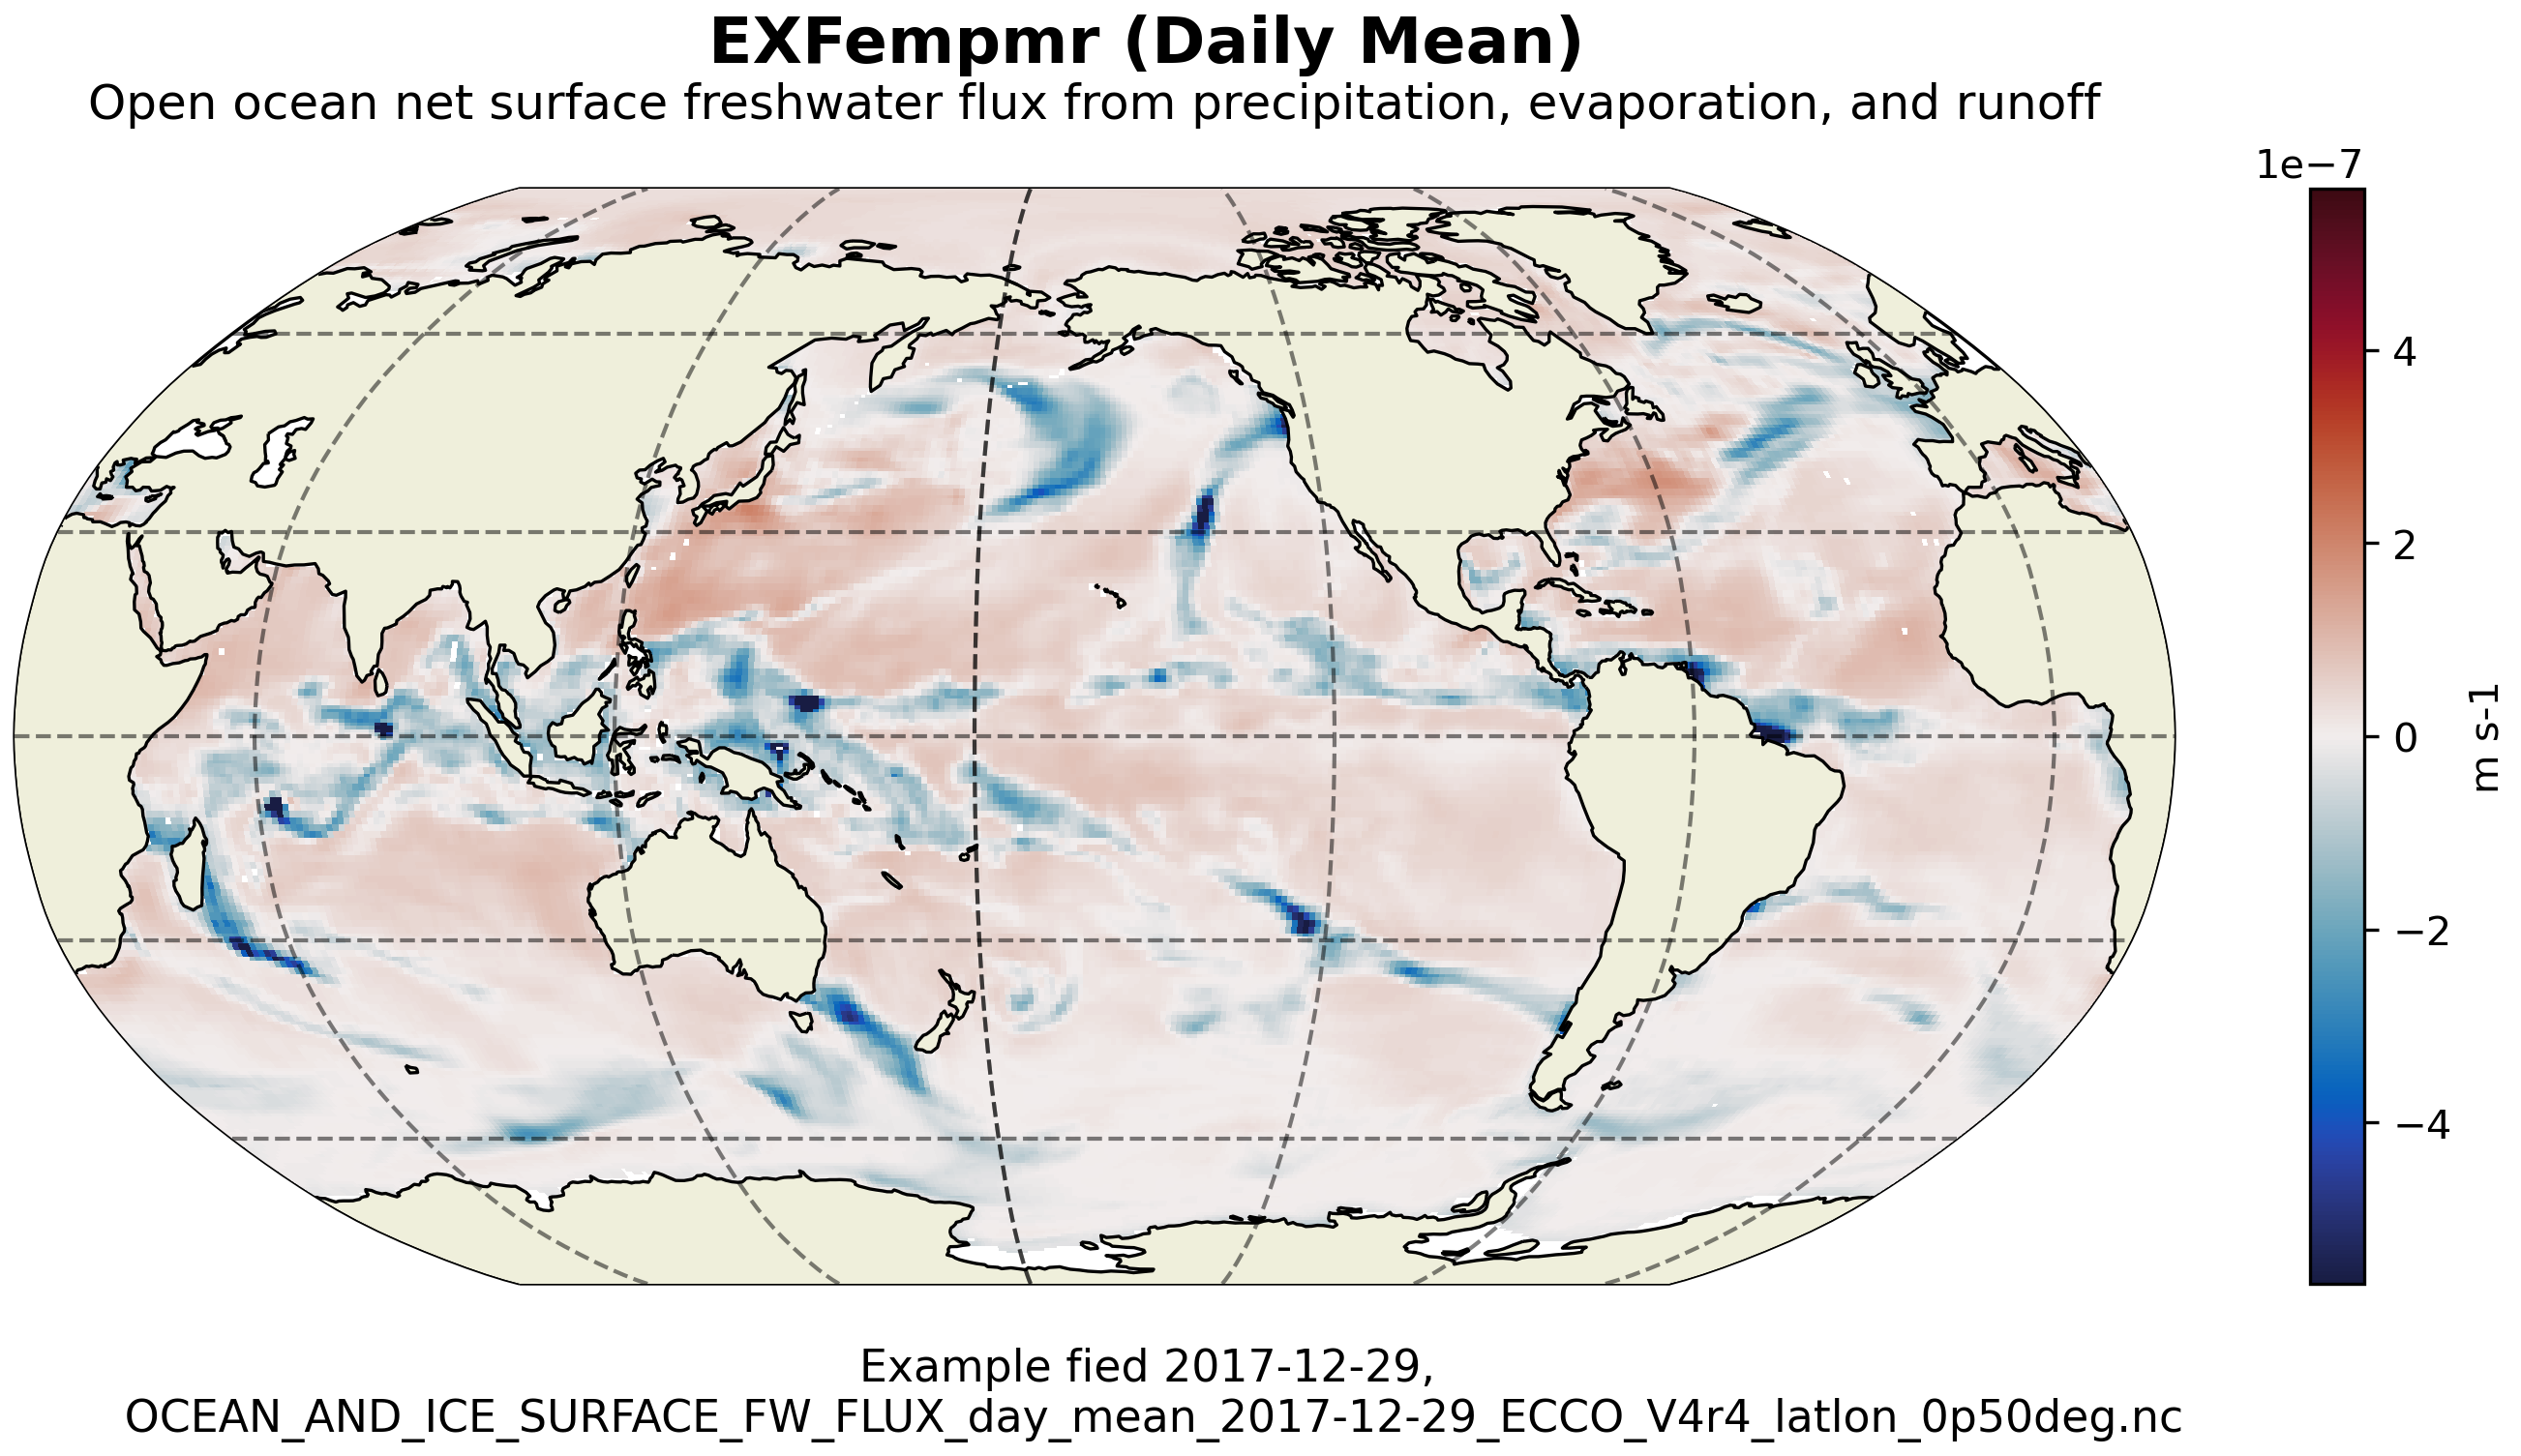
\includegraphics[width=\textwidth]{../images/plots/latlon_plots/Ocean_and_Sea-Ice_Surface_Freshwater_Fluxes/EXFempmr.png}
\caption{Dataset: OCEAN\_AND\_ICE\_SURFACE\_FW\_FLUX Variable: EXFempmr}
\label{tab:table-OCEAN_AND_ICE_SURFACE_FW_FLUX_EXFempmr-Plot}
\end{figure}
\pagebreak
\subsubsection{Latlon Variable EXFevap}
\begin{longtable}{|p{0.06\textwidth}|p{0.41\textwidth}|p{0.39\textwidth}|p{0.06\textwidth}|}
\caption{CDL description of OCEAN\_AND\_ICE\_SURFACE\_FW\_FLUX's EXFevap variable}
\label{tab:table-OCEAN_AND_ICE_SURFACE_FW_FLUX_EXFevap} \\ 
\hline \endhead \hline \endfoot
\rowcolor{lightgray} \textbf{Storage Type} & \textbf{Variable Name} & \textbf{Description} & \textbf{Unit} \\ \hline
float32 & EXFevap & Open ocean evaporation rate & m s-1 \\ \hline
\rowcolor{lightgray}  \multicolumn{4}{|p{1.00\textwidth}|}{\textbf{CDL Description}} \\ \hline
\multicolumn{4}{|p{1.00\textwidth}|}{\makecell{\parbox{1\textwidth}{float32 EXFevap(time, latitude, longitude)\\
\hspace*{0.5cm}EXFevap: \_FillValue = 9.96921e+36\\
\hspace*{0.5cm}EXFevap: coverage\_content\_type = modelResult\\
\hspace*{0.5cm}EXFevap: direction = >0 increases salinity (SALT)\\
\hspace*{0.5cm}EXFevap: long\_name = Open ocean evaporation rate\\
\hspace*{0.5cm}EXFevap: standard\_name = lwe\_water\_evaporation\_rate\\
\hspace*{0.5cm}EXFevap: units = m s: 1\\
\hspace*{0.5cm}EXFevap: coordinates = time\\
\hspace*{0.5cm}EXFevap: valid\_min = : 1.0958113705328287e: 07\\
\hspace*{0.5cm}EXFevap: valid\_max = 7.090054623404285e: 07}}} \\ \hline
\rowcolor{lightgray} \multicolumn{4}{|p{1.00\textwidth}|}{\textbf{Comments}} \\ \hline
\multicolumn{4}{|p{1\textwidth}|}{Evaporation rate per unit area of open water (not covered by sea-ice). Note: calculated using the bulk formula following Large and Yeager (2004) NCAR/TN-460+STR.} \\ \hline
\end{longtable}

\begin{figure}[H]
\centering
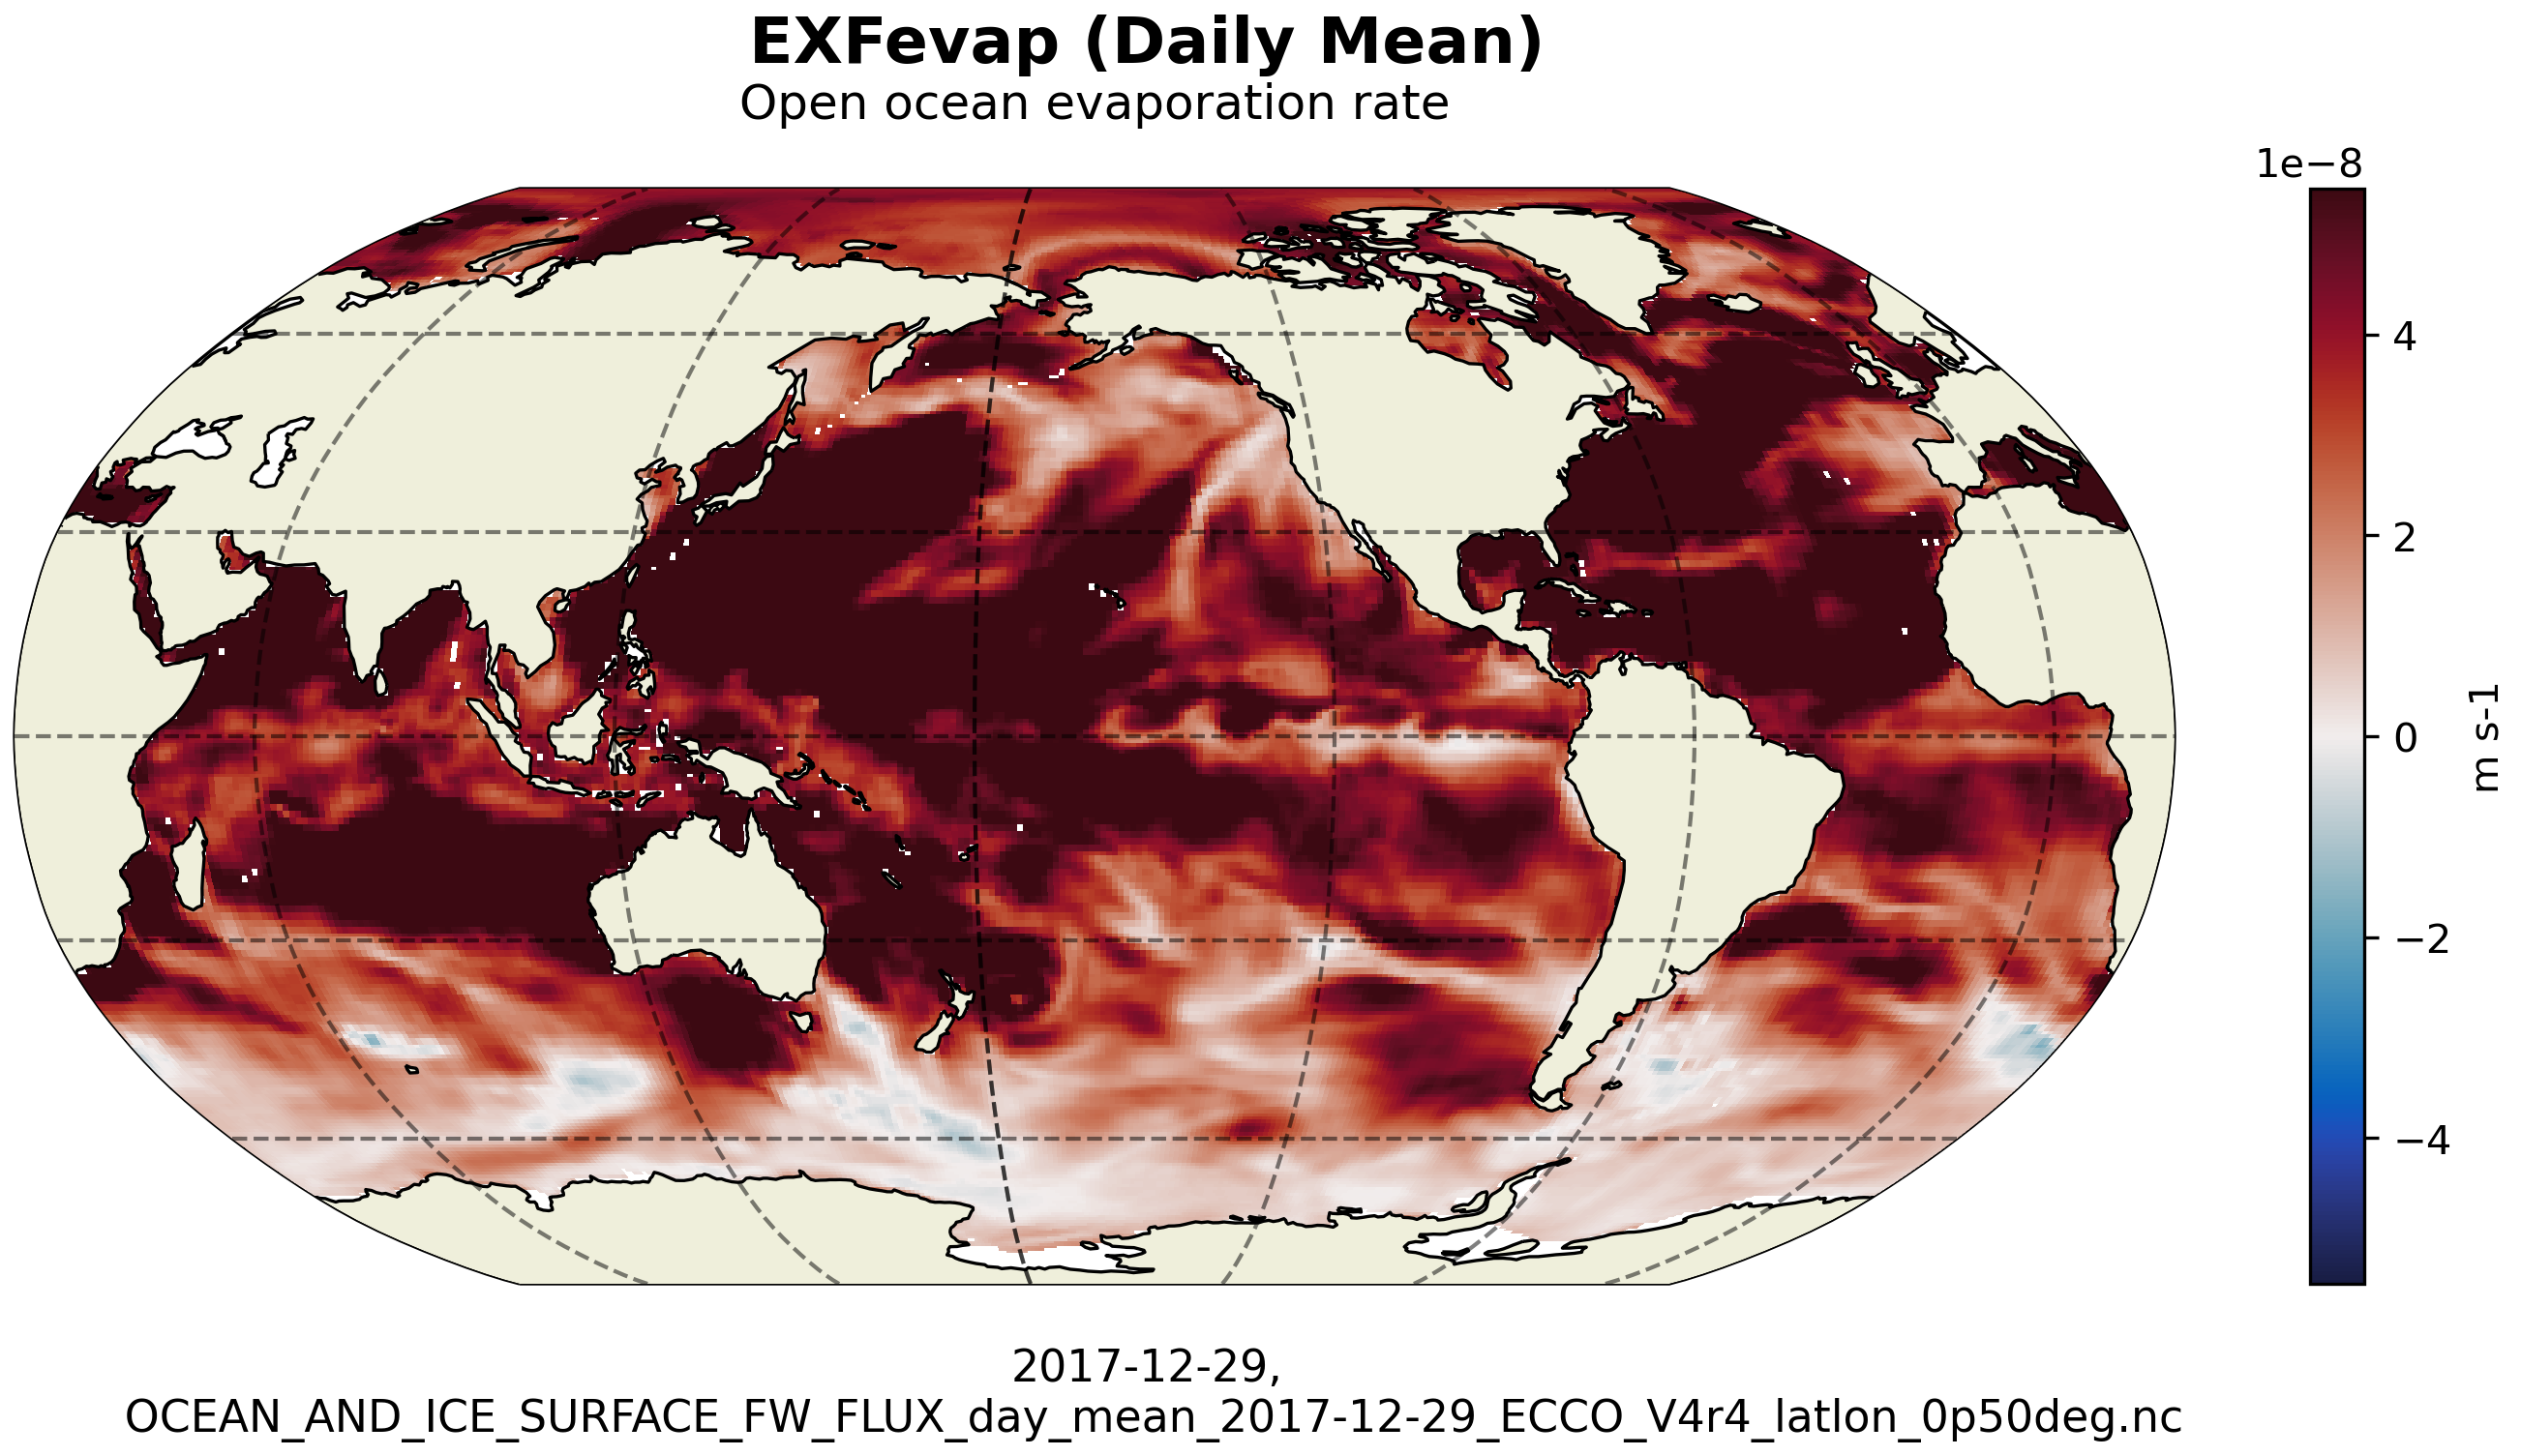
\includegraphics[width=\textwidth]{../images/plots/latlon_plots/Ocean_and_Sea-Ice_Surface_Freshwater_Fluxes/EXFevap.png}
\caption{Dataset: OCEAN\_AND\_ICE\_SURFACE\_FW\_FLUX Variable: EXFevap}
\label{tab:table-OCEAN_AND_ICE_SURFACE_FW_FLUX_EXFevap-Plot}
\end{figure}
\pagebreak
\subsubsection{Latlon Variable EXFpreci}
\begin{longtable}{|p{0.06\textwidth}|p{0.41\textwidth}|p{0.39\textwidth}|p{0.06\textwidth}|}
\caption{CDL description of OCEAN\_AND\_ICE\_SURFACE\_FW\_FLUX's EXFpreci variable}
\label{tab:table-OCEAN_AND_ICE_SURFACE_FW_FLUX_EXFpreci} \\ 
\hline \endhead \hline \endfoot
\rowcolor{lightgray} \textbf{Storage Type} & \textbf{Variable Name} & \textbf{Description} & \textbf{Unit} \\ \hline
float32 & EXFpreci & Precipitation rate & m s-1 \\ \hline
\rowcolor{lightgray}  \multicolumn{4}{|p{1.00\textwidth}|}{\textbf{CDL Description}} \\ \hline
\multicolumn{4}{|p{1.00\textwidth}|}{\makecell{\parbox{1\textwidth}{float32 EXFpreci(time, latitude, longitude)\\
\hspace*{0.5cm}EXFpreci: \_FillValue = 9.96921e+36\\
\hspace*{0.5cm}EXFpreci: coverage\_content\_type = modelResult\\
\hspace*{0.5cm}EXFpreci: direction = >0 increases salinity (SALT)\\
\hspace*{0.5cm}EXFpreci: long\_name = Precipitation rate\\
\hspace*{0.5cm}EXFpreci: standard\_name = lwe\_precipitation\_rate\\
\hspace*{0.5cm}EXFpreci: units = m s: 1\\
\hspace*{0.5cm}EXFpreci: coordinates = time\\
\hspace*{0.5cm}EXFpreci: valid\_min = : 1.4860395936011628e: 07\\
\hspace*{0.5cm}EXFpreci: valid\_max = 8.317776519106701e: 06}}} \\ \hline
\rowcolor{lightgray} \multicolumn{4}{|p{1.00\textwidth}|}{\textbf{Comments}} \\ \hline
\multicolumn{4}{|p{1\textwidth}|}{Precipitation rate. Note: sum of ERA-Interim precipitation and the control adjustment from ocean state estimation.} \\ \hline
\end{longtable}

\begin{figure}[H]
\centering
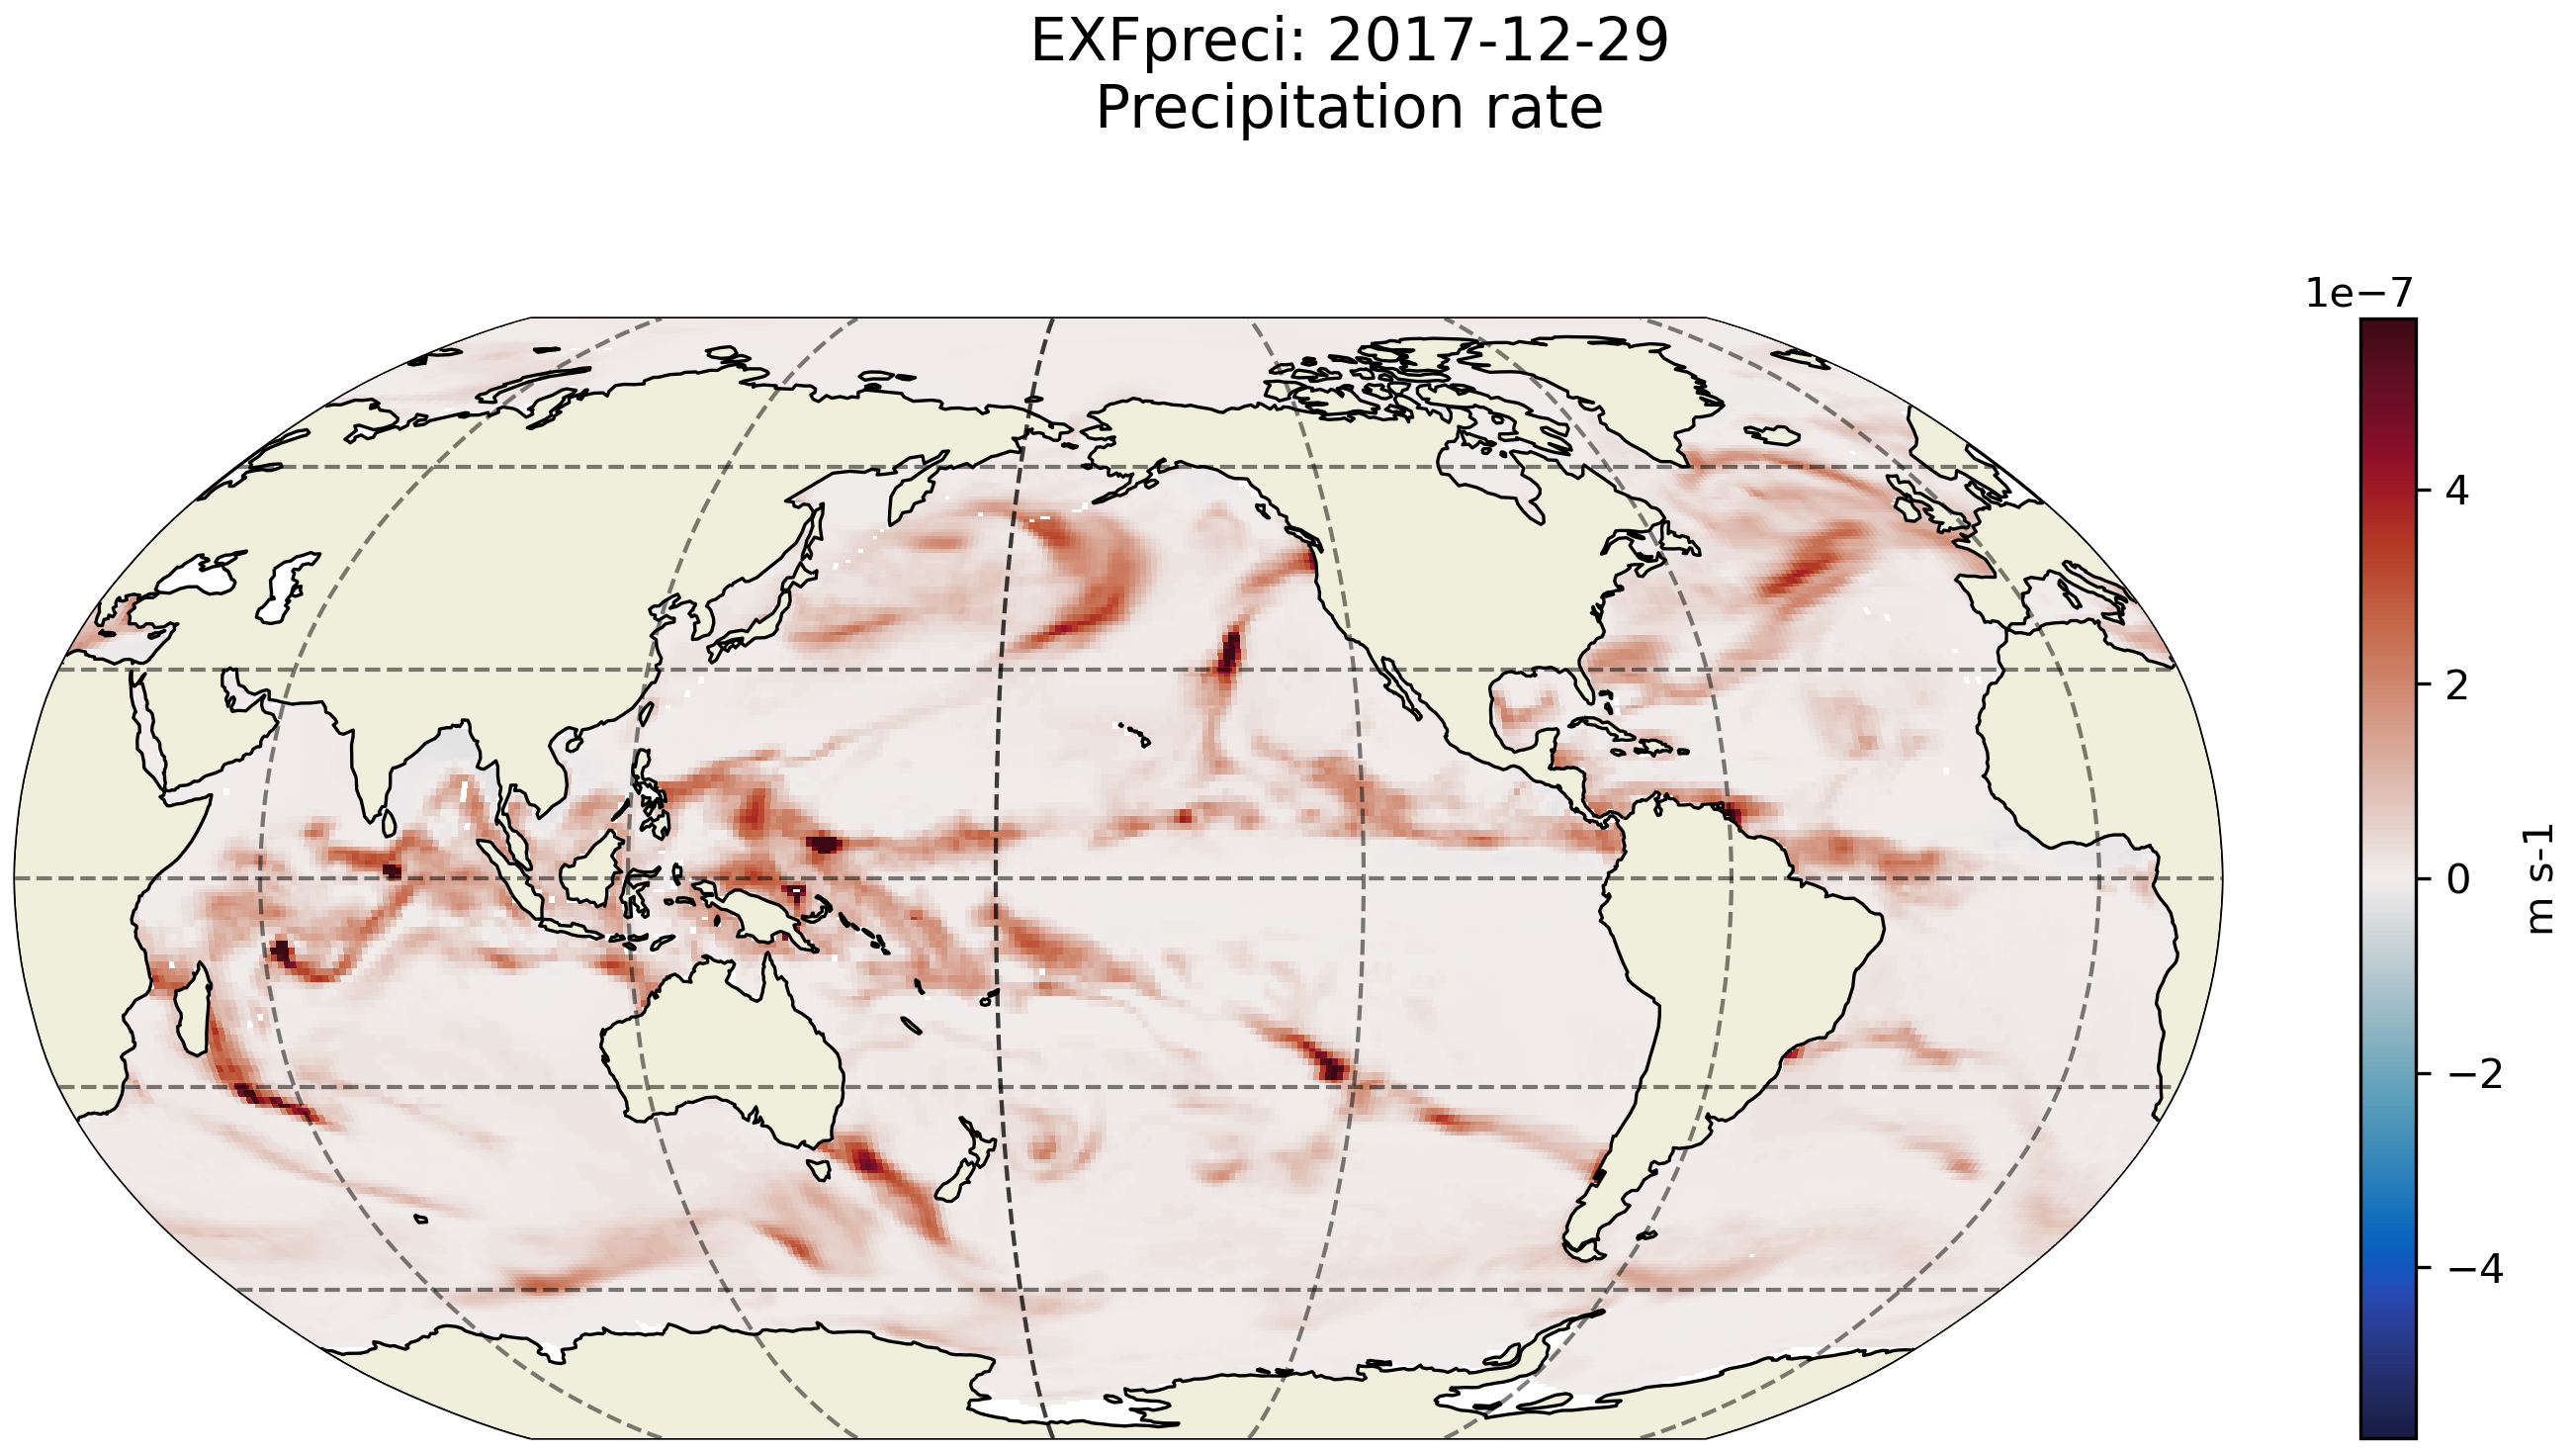
\includegraphics[width=\textwidth]{../images/plots/latlon_plots/Ocean_and_Sea-Ice_Surface_Freshwater_Fluxes/EXFpreci.png}
\caption{Dataset: OCEAN\_AND\_ICE\_SURFACE\_FW\_FLUX Variable: EXFpreci}
\label{tab:table-OCEAN_AND_ICE_SURFACE_FW_FLUX_EXFpreci-Plot}
\end{figure}
\pagebreak
\subsubsection{Latlon Variable EXFroff}
\begin{longtable}{|p{0.06\textwidth}|p{0.41\textwidth}|p{0.39\textwidth}|p{0.06\textwidth}|}
\caption{CDL description of OCEAN\_AND\_ICE\_SURFACE\_FW\_FLUX's EXFroff variable}
\label{tab:table-OCEAN_AND_ICE_SURFACE_FW_FLUX_EXFroff} \\ 
\hline \endhead \hline \endfoot
\rowcolor{lightgray} \textbf{Storage Type} & \textbf{Variable Name} & \textbf{Description} & \textbf{Unit} \\ \hline
float32 & EXFroff & River runoff & m s-1 \\ \hline
\rowcolor{lightgray}  \multicolumn{4}{|p{1.00\textwidth}|}{\textbf{CDL Description}} \\ \hline
\multicolumn{4}{|p{1.00\textwidth}|}{\makecell{\parbox{1\textwidth}{float32 EXFroff(time, latitude, longitude)\\
\hspace*{0.5cm}EXFroff: \_FillValue = 9.96921e+36\\
\hspace*{0.5cm}EXFroff: coverage\_content\_type = modelResult\\
\hspace*{0.5cm}EXFroff: direction = >0 increases salinity (SALT)\\
\hspace*{0.5cm}EXFroff: long\_name = River runoff\\
\hspace*{0.5cm}EXFroff: standard\_name = surface\_runoff\_flux\\
\hspace*{0.5cm}EXFroff: units = m s: 1\\
\hspace*{0.5cm}EXFroff: coordinates = time\\
\hspace*{0.5cm}EXFroff: valid\_min = 0.0\\
\hspace*{0.5cm}EXFroff: valid\_max = 4.185612397122895e: 06}}} \\ \hline
\rowcolor{lightgray} \multicolumn{4}{|p{1.00\textwidth}|}{\textbf{Comments}} \\ \hline
\multicolumn{4}{|p{1\textwidth}|}{River runoff freshwater flux. Note: not adjusted by the optimization.} \\ \hline
\end{longtable}

\begin{figure}[H]
\centering
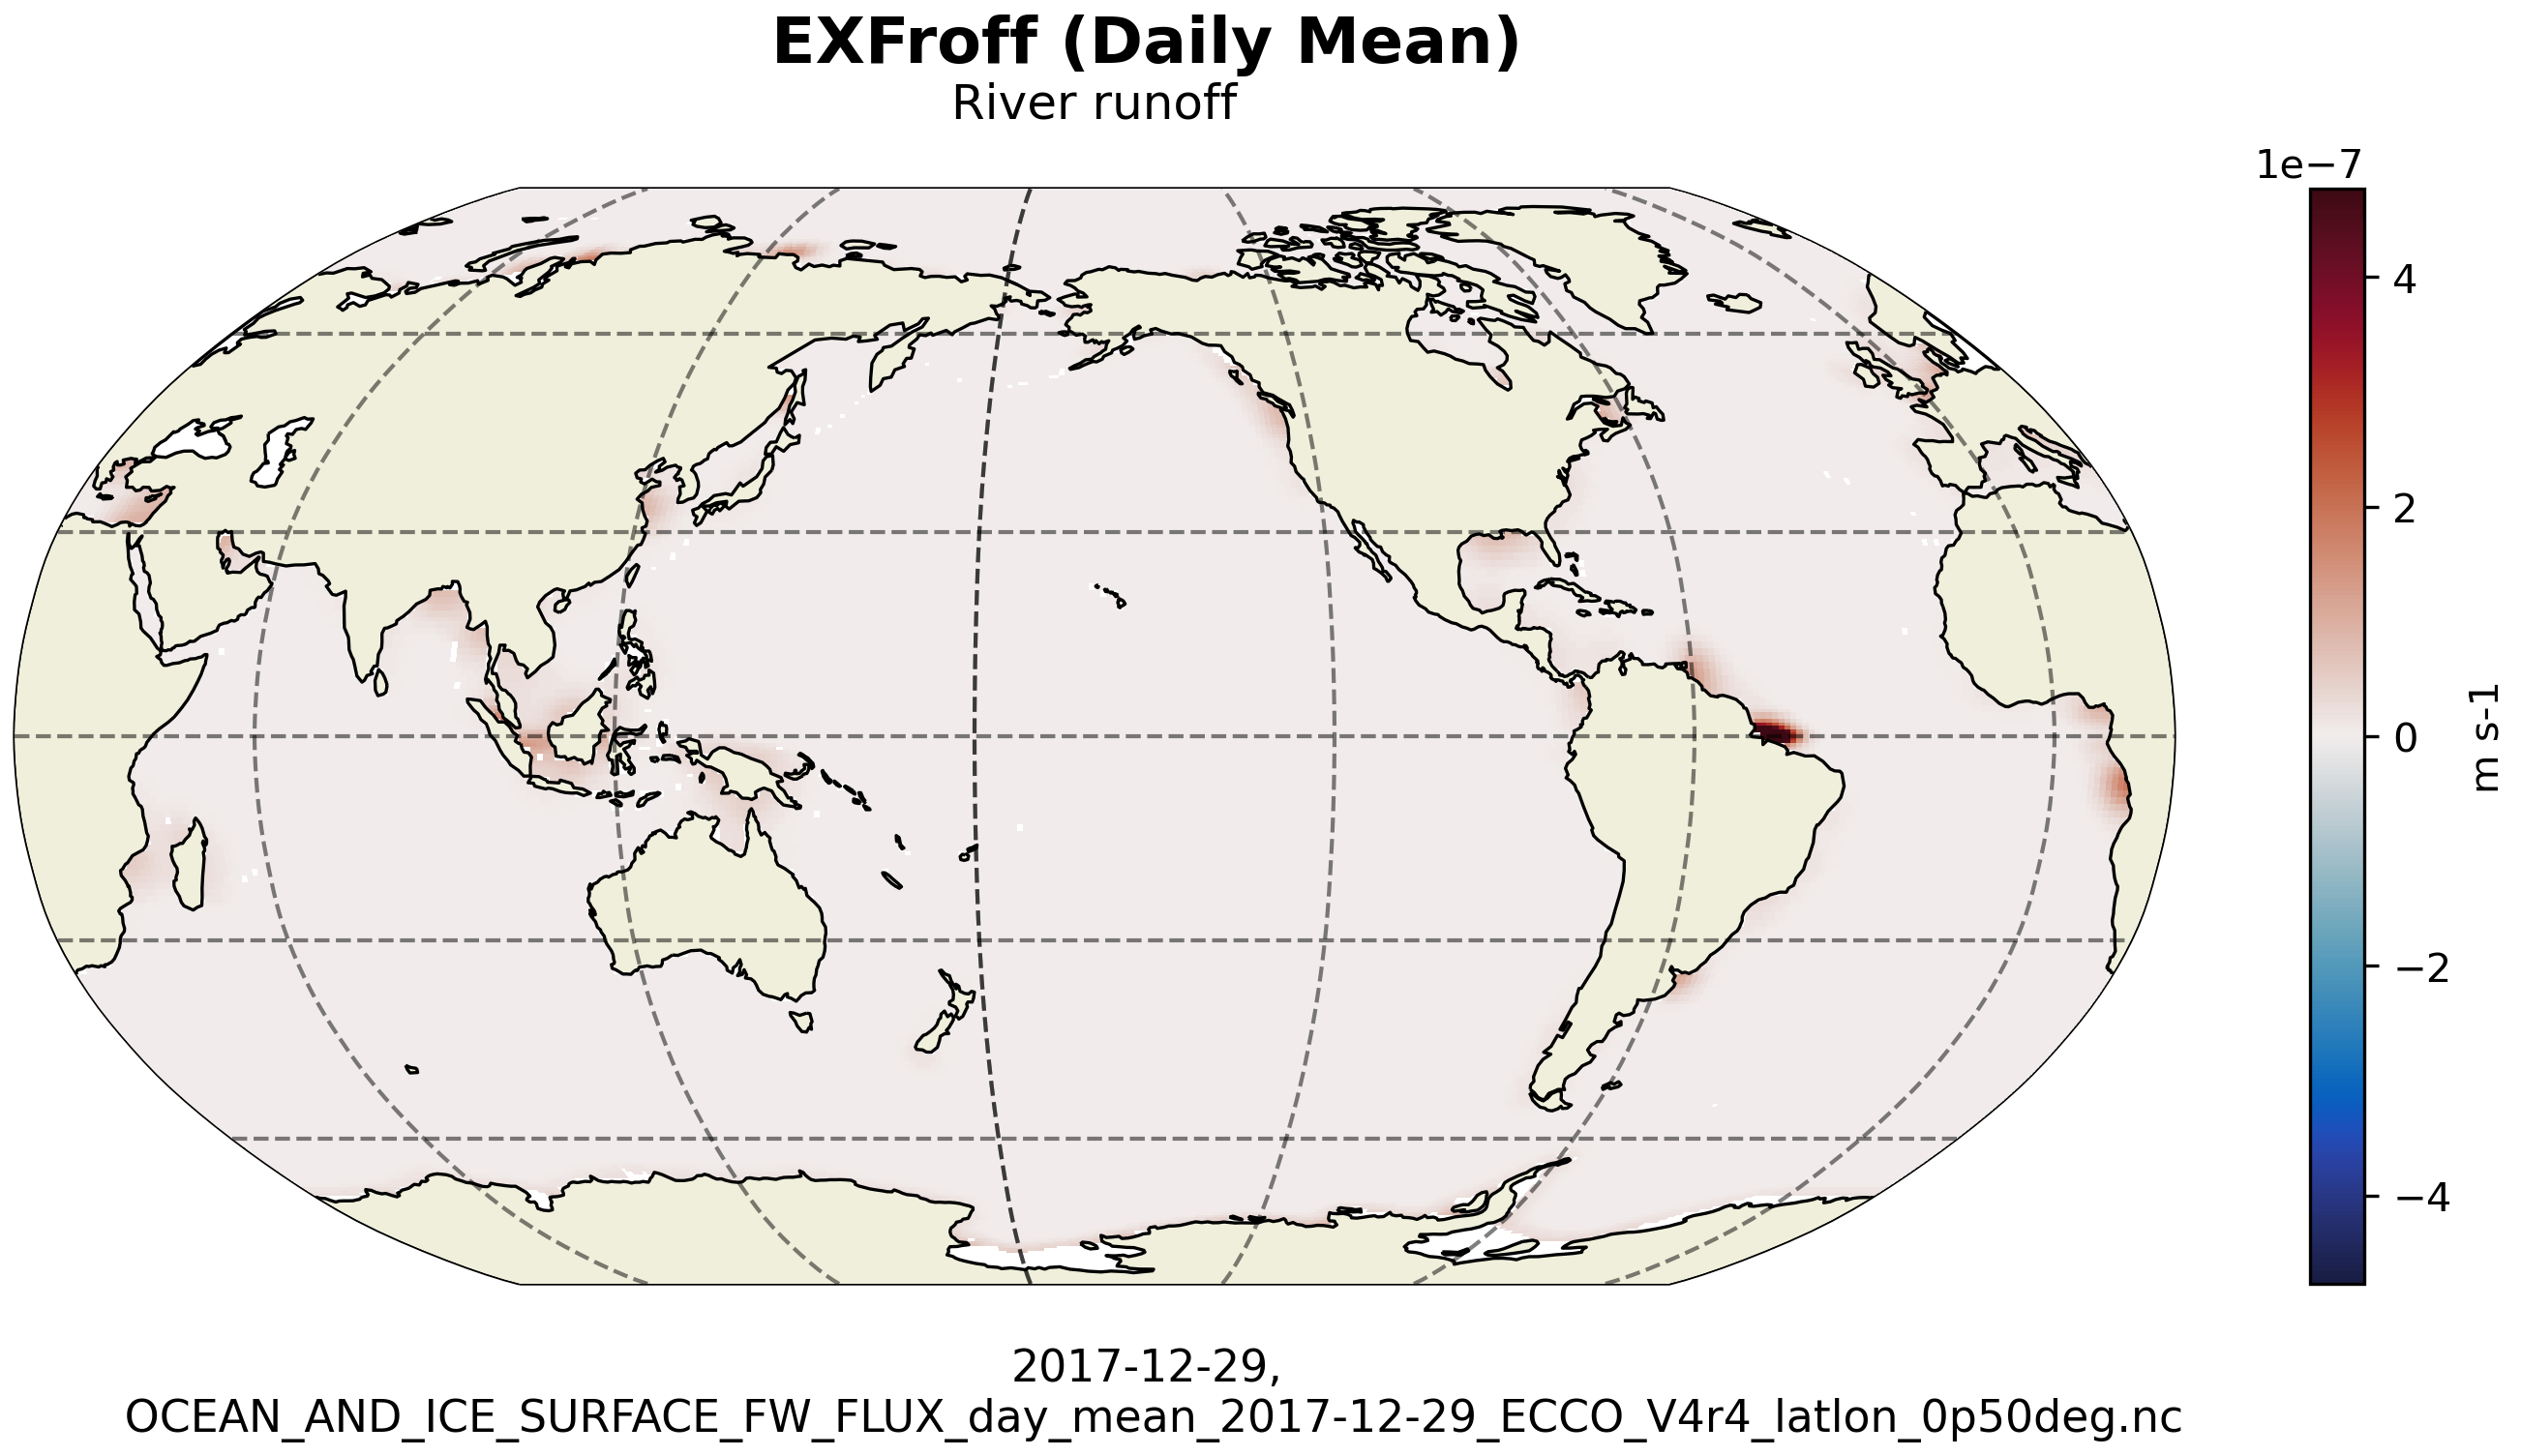
\includegraphics[width=\textwidth]{../images/plots/latlon_plots/Ocean_and_Sea-Ice_Surface_Freshwater_Fluxes/EXFroff.png}
\caption{Dataset: OCEAN\_AND\_ICE\_SURFACE\_FW\_FLUX Variable: EXFroff}
\label{tab:table-OCEAN_AND_ICE_SURFACE_FW_FLUX_EXFroff-Plot}
\end{figure}
\pagebreak
\subsubsection{Latlon Variable SFLUX}
\begin{longtable}{|p{0.06\textwidth}|p{0.41\textwidth}|p{0.39\textwidth}|p{0.06\textwidth}|}
\caption{CDL description of OCEAN\_AND\_ICE\_SURFACE\_FW\_FLUX's SFLUX variable}
\label{tab:table-OCEAN_AND_ICE_SURFACE_FW_FLUX_SFLUX} \\ 
\hline \endhead \hline \endfoot
\rowcolor{lightgray} \textbf{Storage Type} & \textbf{Variable Name} & \textbf{Description} & \textbf{Unit} \\ \hline
float32 & SFLUX & Rate of change of total ocean salinity per m2 accounting for mass fluxes. & g m-2 s-1 \\ \hline
\rowcolor{lightgray}  \multicolumn{4}{|p{1.00\textwidth}|}{\textbf{CDL Description}} \\ \hline
\multicolumn{4}{|p{1.00\textwidth}|}{\makecell{\parbox{1\textwidth}{float32 SFLUX(time, latitude, longitude)\\
\hspace*{0.5cm}SFLUX: \_FillValue = 9.96921e+36\\
\hspace*{0.5cm}SFLUX: coverage\_content\_type = modelResult\\
\hspace*{0.5cm}SFLUX: direction = >0 increases salinity (SALT)\\
\hspace*{0.5cm}SFLUX: long\_name = Rate of change of total ocean salinity per m2 accounting for mass fluxes.\\
\hspace*{0.5cm}SFLUX: units = g m: 2 s: 1\\
\hspace*{0.5cm}SFLUX: coordinates = time\\
\hspace*{0.5cm}SFLUX: valid\_min = : 0.06244903802871704\\
\hspace*{0.5cm}SFLUX: valid\_max = 0.010570422746241093}}} \\ \hline
\rowcolor{lightgray} \multicolumn{4}{|p{1.00\textwidth}|}{\textbf{Comments}} \\ \hline
\multicolumn{4}{|p{1\textwidth}|}{The rate of change of total ocean salinity due to freshwater fluxes across the liquid surface and the addition or removal of mass. Note: the global area integral of SFLUX matches the time-derivative of total ocean salinity (psu s-1). Unlike oceFWflx, SFLUX includes the contribution to the total ocean salinity from changing ocean mass (e.g. from the addition or removal of freshwater in oceFWflx). } \\ \hline
\end{longtable}

\begin{figure}[H]
\centering
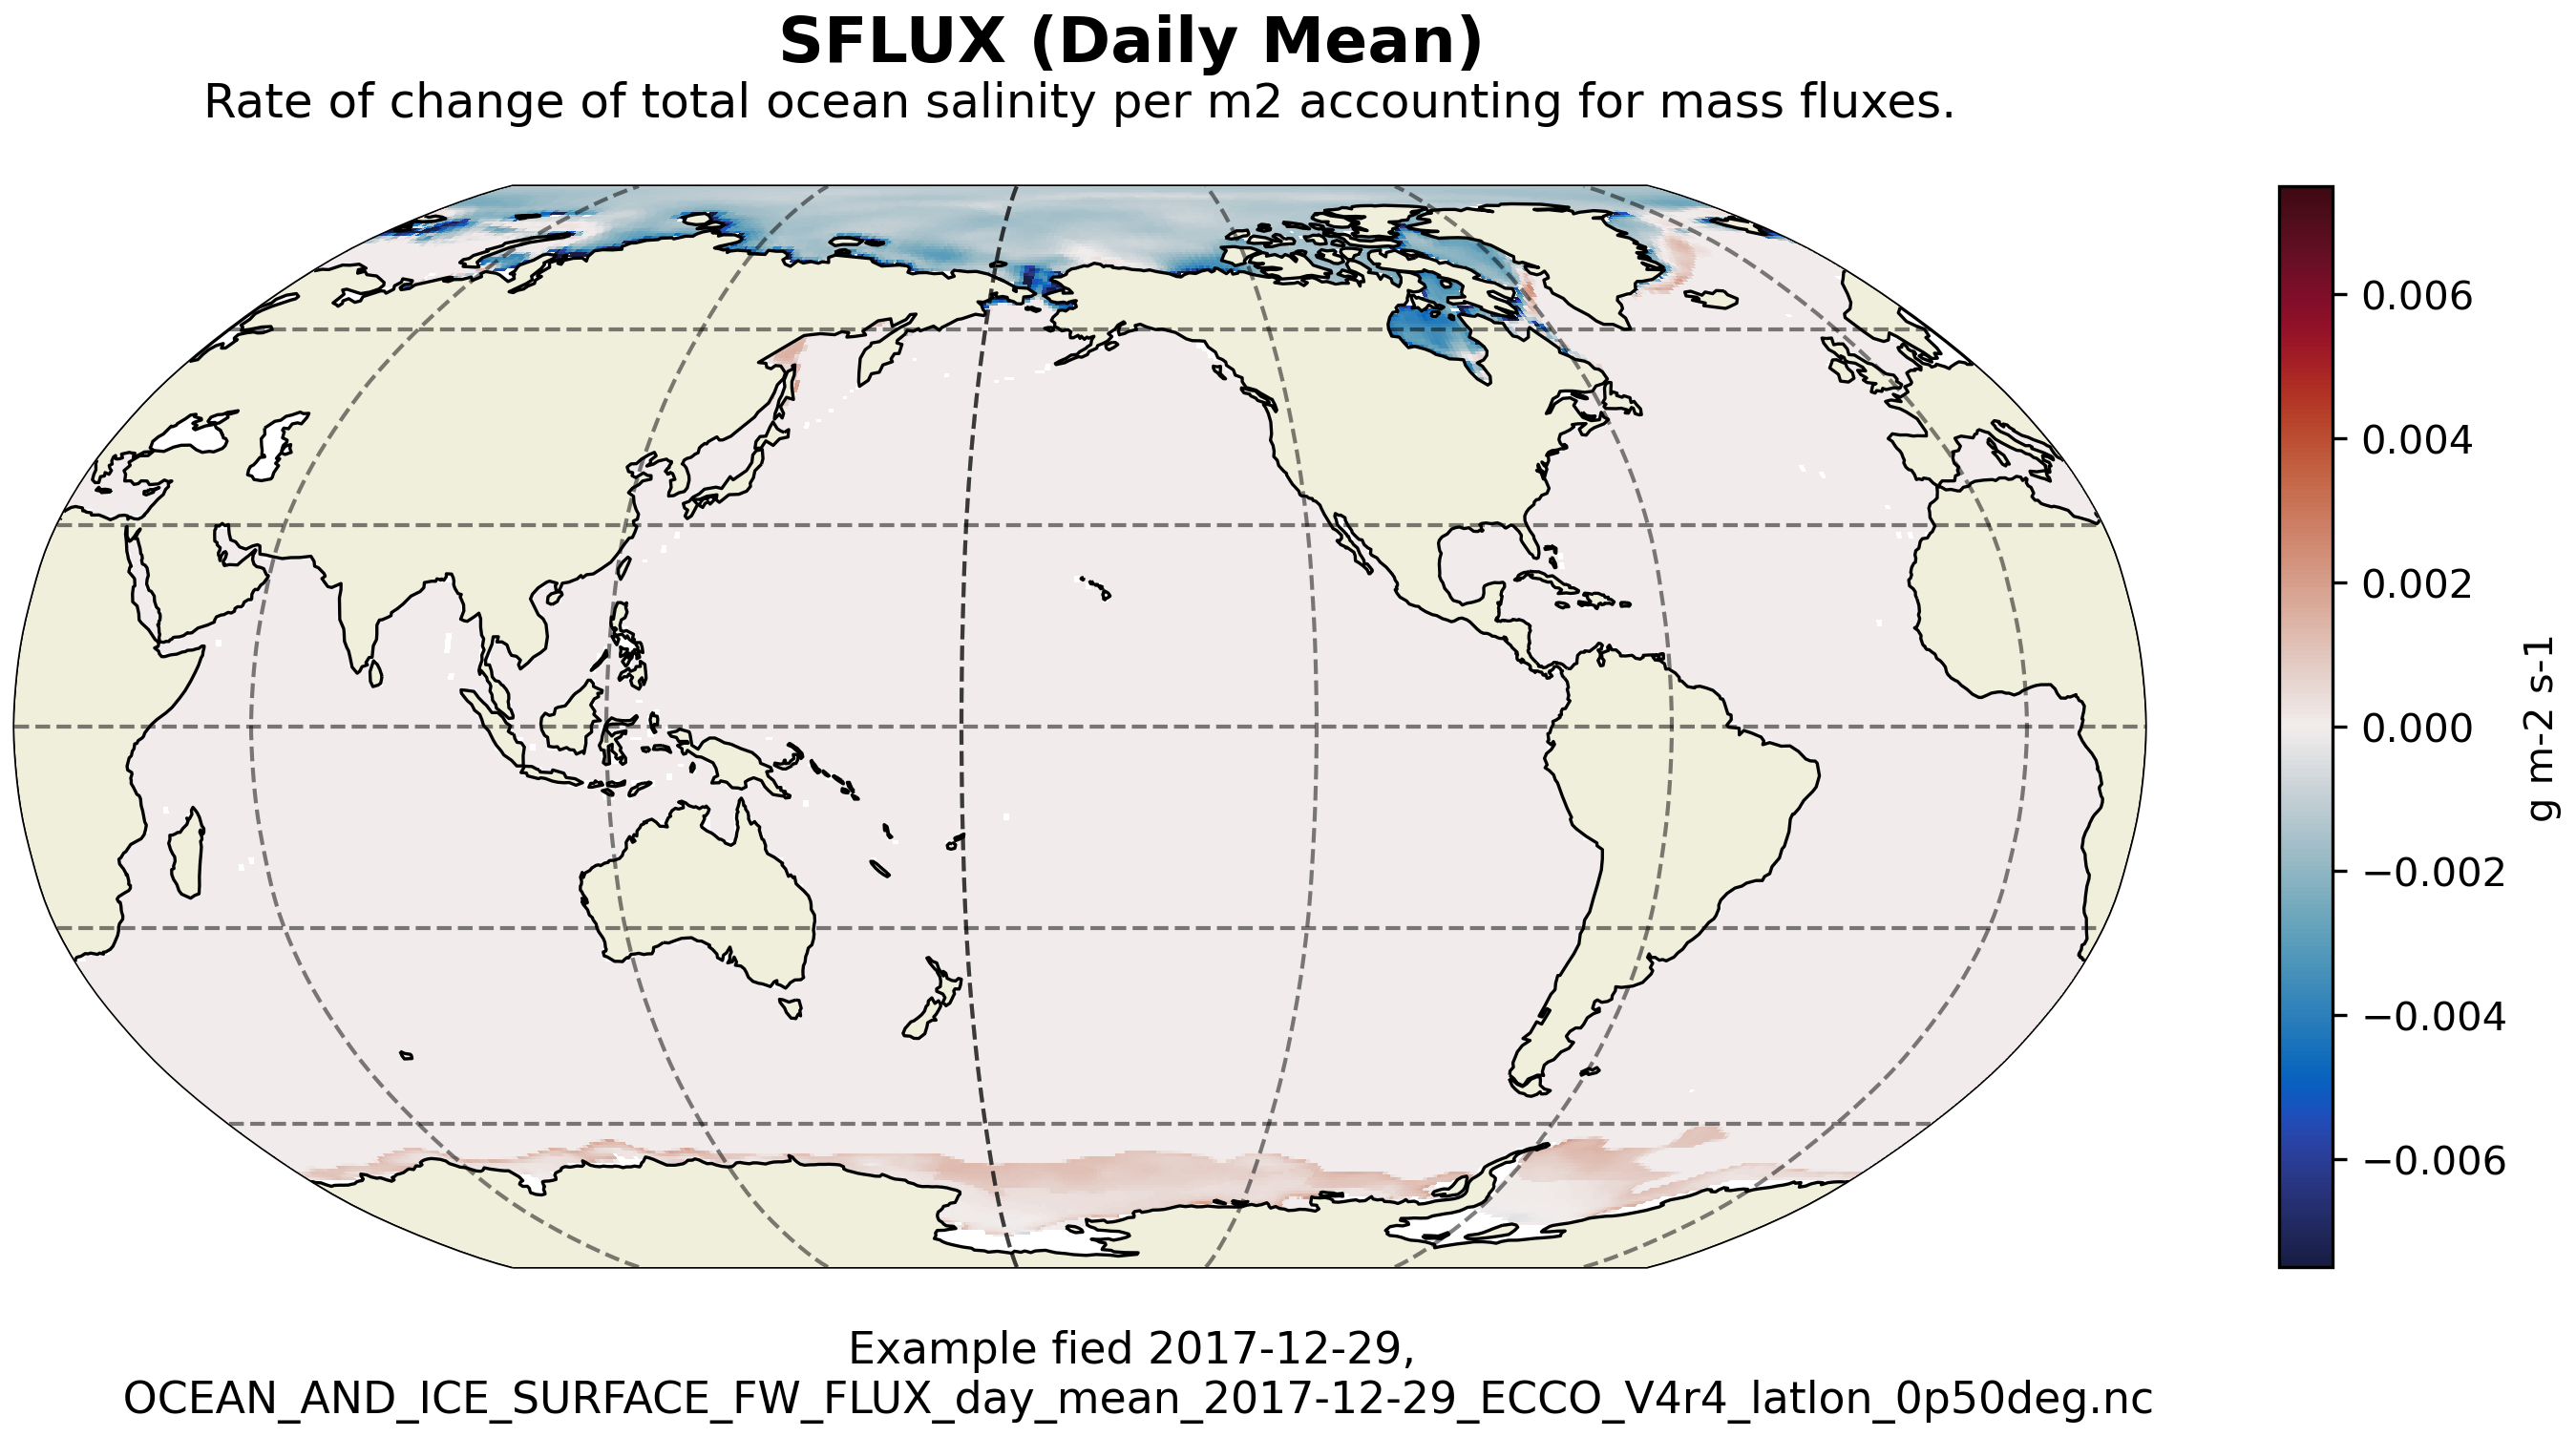
\includegraphics[width=\textwidth]{../images/plots/latlon_plots/Ocean_and_Sea-Ice_Surface_Freshwater_Fluxes/SFLUX.png}
\caption{Dataset: OCEAN\_AND\_ICE\_SURFACE\_FW\_FLUX Variable: SFLUX}
\label{tab:table-OCEAN_AND_ICE_SURFACE_FW_FLUX_SFLUX-Plot}
\end{figure}
\pagebreak
\subsubsection{Latlon Variable SIacSubl}
\begin{longtable}{|p{0.06\textwidth}|p{0.41\textwidth}|p{0.39\textwidth}|p{0.06\textwidth}|}
\caption{CDL description of OCEAN\_AND\_ICE\_SURFACE\_FW\_FLUX's SIacSubl variable}
\label{tab:table-OCEAN_AND_ICE_SURFACE_FW_FLUX_SIacSubl} \\ 
\hline \endhead \hline \endfoot
\rowcolor{lightgray} \textbf{Storage Type} & \textbf{Variable Name} & \textbf{Description} & \textbf{Unit} \\ \hline
float32 & SIacSubl & Freshwater flux to the atmosphere due to sublimation-deposition of snow or ice & kg m-2 s-1 \\ \hline
\rowcolor{lightgray}  \multicolumn{4}{|p{1.00\textwidth}|}{\textbf{CDL Description}} \\ \hline
\multicolumn{4}{|p{1.00\textwidth}|}{\makecell{\parbox{1\textwidth}{float32 SIacSubl(time, latitude, longitude)\\
\hspace*{0.5cm}SIacSubl: \_FillValue = 9.96921e+36\\
\hspace*{0.5cm}SIacSubl: coverage\_content\_type = modelResult\\
\hspace*{0.5cm}SIacSubl: direction = >0 decreases snow or sea: ice thickness (HSNOW or HEFF)\\
\hspace*{0.5cm}SIacSubl: long\_name = Freshwater flux to the atmosphere due to sublimation: deposition of snow or ice\\
\hspace*{0.5cm}SIacSubl: standard\_name = water\_sublimation\_flux\\
\hspace*{0.5cm}SIacSubl: units = kg m: 2 s: 1\\
\hspace*{0.5cm}SIacSubl: coordinates = time\\
\hspace*{0.5cm}SIacSubl: valid\_min = 0.0\\
\hspace*{0.5cm}SIacSubl: valid\_max = 7.735946564935148e: 05}}} \\ \hline
\rowcolor{lightgray} \multicolumn{4}{|p{1.00\textwidth}|}{\textbf{Comments}} \\ \hline
\multicolumn{4}{|p{1\textwidth}|}{Freshwater flux to the atmosphere due to sublimation-deposition of snow or ice. Positive values imply sublimation from ice/snow to vapor, negative values imply deposition from atmospheric moisture} \\ \hline
\end{longtable}

\begin{figure}[H]
\centering
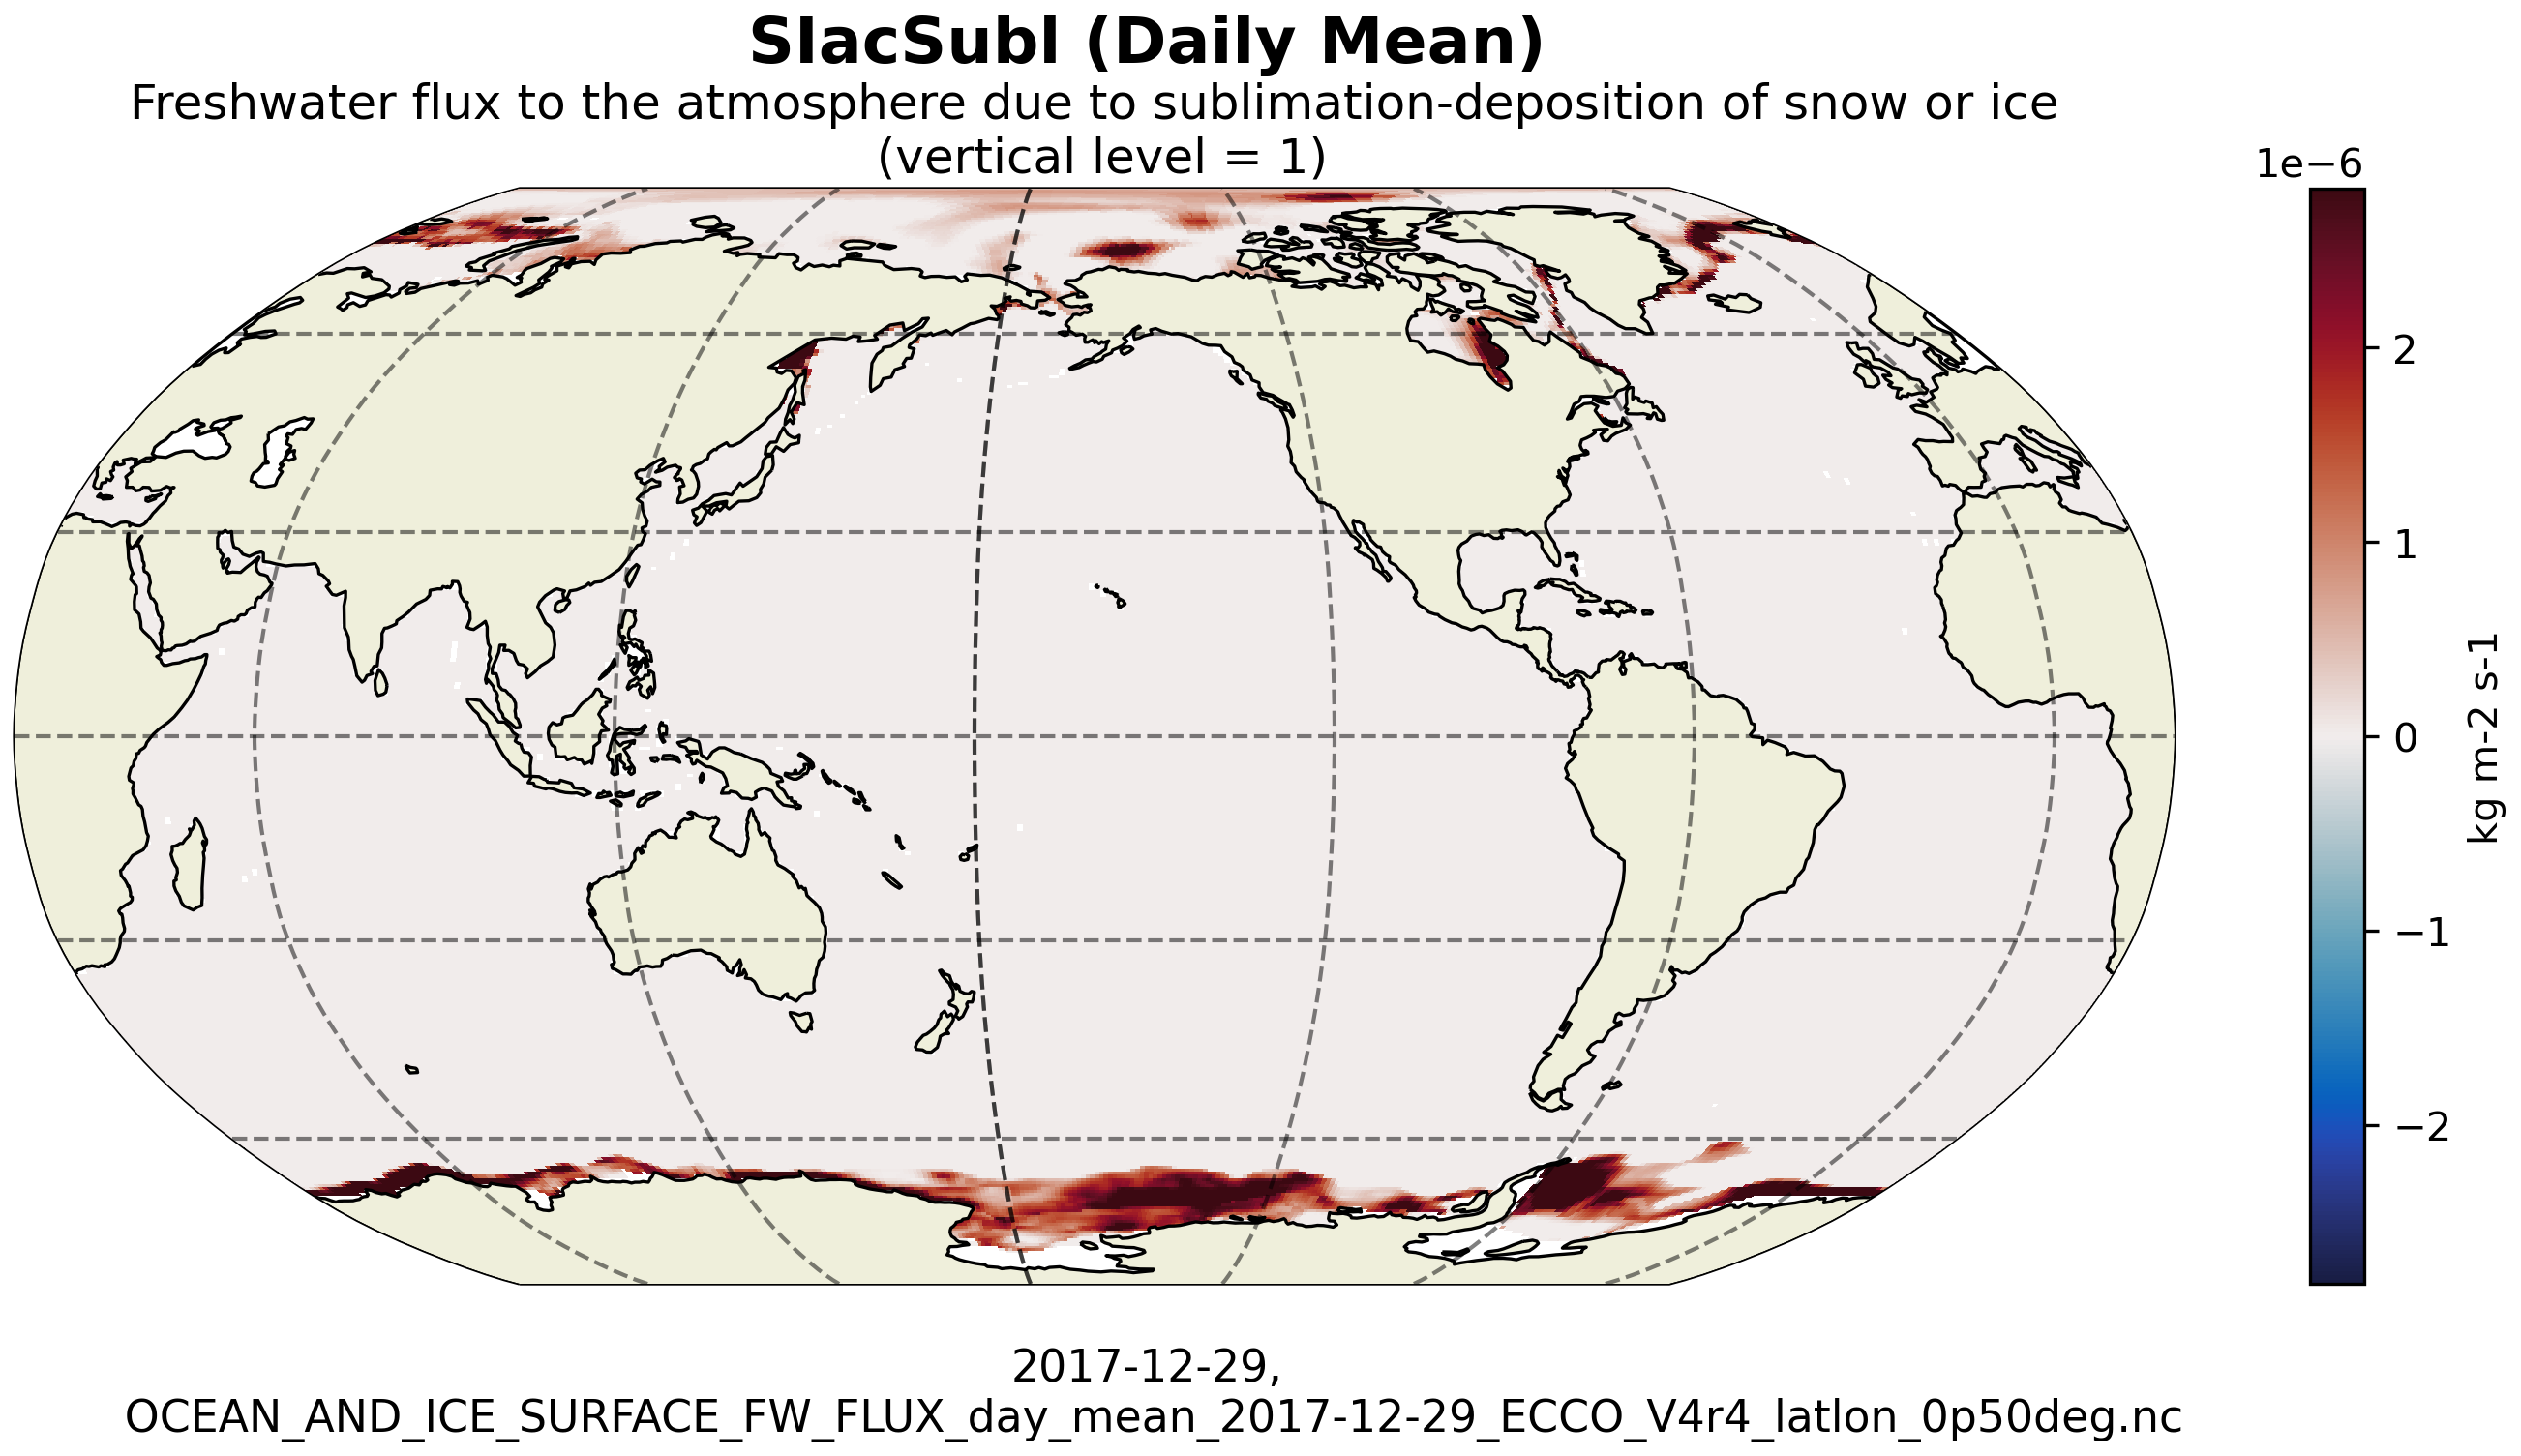
\includegraphics[width=\textwidth]{../images/plots/latlon_plots/Ocean_and_Sea-Ice_Surface_Freshwater_Fluxes/SIacSubl.png}
\caption{Dataset: OCEAN\_AND\_ICE\_SURFACE\_FW\_FLUX Variable: SIacSubl}
\label{tab:table-OCEAN_AND_ICE_SURFACE_FW_FLUX_SIacSubl-Plot}
\end{figure}
\pagebreak
\subsubsection{Latlon Variable SIatmFW}
\begin{longtable}{|p{0.06\textwidth}|p{0.41\textwidth}|p{0.39\textwidth}|p{0.06\textwidth}|}
\caption{CDL description of OCEAN\_AND\_ICE\_SURFACE\_FW\_FLUX's SIatmFW variable}
\label{tab:table-OCEAN_AND_ICE_SURFACE_FW_FLUX_SIatmFW} \\ 
\hline \endhead \hline \endfoot
\rowcolor{lightgray} \textbf{Storage Type} & \textbf{Variable Name} & \textbf{Description} & \textbf{Unit} \\ \hline
float32 & SIatmFW & Net freshwater flux into the open ocean, sea-ice, and snow & kg m-2 s-1 \\ \hline
\rowcolor{lightgray}  \multicolumn{4}{|p{1.00\textwidth}|}{\textbf{CDL Description}} \\ \hline
\multicolumn{4}{|p{1.00\textwidth}|}{\makecell{\parbox{1\textwidth}{float32 SIatmFW(time, latitude, longitude)\\
\hspace*{0.5cm}SIatmFW: \_FillValue = 9.96921e+36\\
\hspace*{0.5cm}SIatmFW: coverage\_content\_type = modelResult\\
\hspace*{0.5cm}SIatmFW: direction = >0 decreases salinity (SALT)\\
\hspace*{0.5cm}SIatmFW: long\_name = Net freshwater flux into the open ocean\\
sea: ice\\
and snow\\
\hspace*{0.5cm}SIatmFW: standard\_name = surface\_downward\_water\_flux\\
\hspace*{0.5cm}SIatmFW: units = kg m: 2 s: 1\\
\hspace*{0.5cm}SIatmFW: coordinates = time\\
\hspace*{0.5cm}SIatmFW: valid\_min = : 0.00043017856660299003\\
\hspace*{0.5cm}SIatmFW: valid\_max = 0.008299433626234531}}} \\ \hline
\rowcolor{lightgray} \multicolumn{4}{|p{1.00\textwidth}|}{\textbf{Comments}} \\ \hline
\multicolumn{4}{|p{1\textwidth}|}{Net freshwater flux into the combined liquid ocean, sea-ice, and snow reservoirs from the atmosphere and runoff. Note: freshwater fluxes BETWEEN the liquid ocean and sea-ice or snow reservoirs do not contribute to SIatmFW. SIatmFW counts all fluxes to/from the atmosphere that change the TOTAL freshwater stored in the combined liquid ocean, sea-ice, and snow reservoirs.} \\ \hline
\end{longtable}

\begin{figure}[H]
\centering
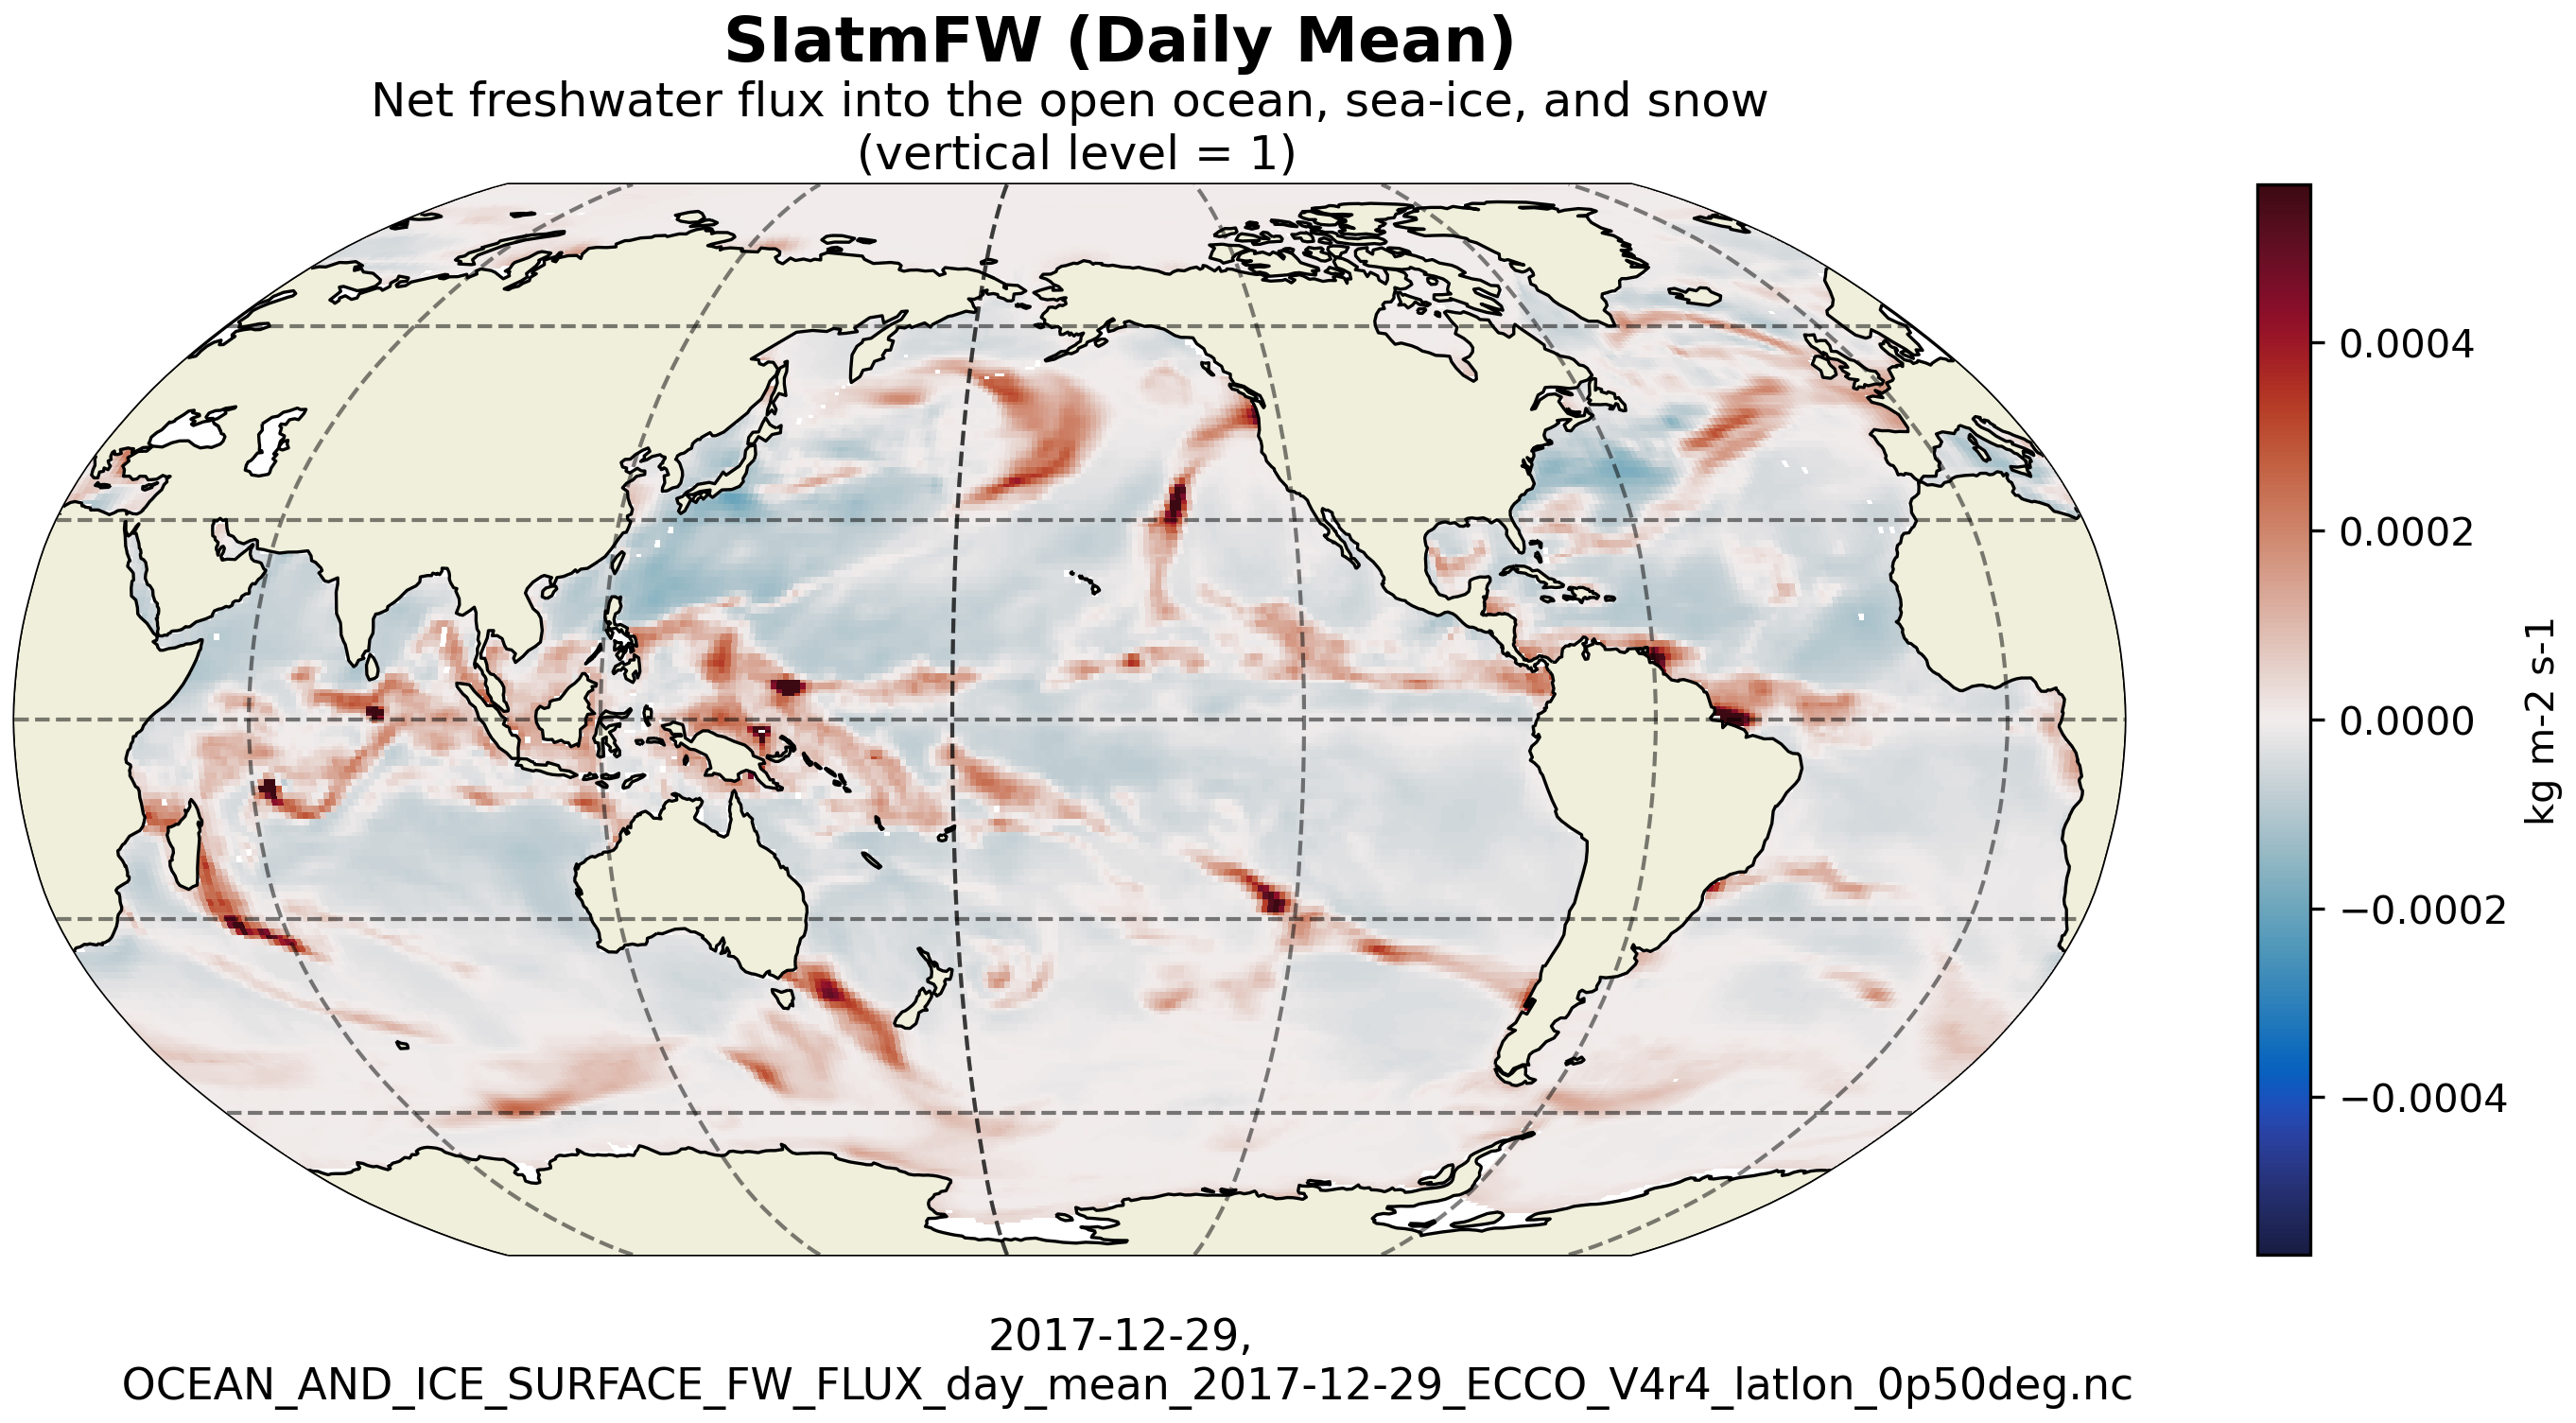
\includegraphics[width=\textwidth]{../images/plots/latlon_plots/Ocean_and_Sea-Ice_Surface_Freshwater_Fluxes/SIatmFW.png}
\caption{Dataset: OCEAN\_AND\_ICE\_SURFACE\_FW\_FLUX Variable: SIatmFW}
\label{tab:table-OCEAN_AND_ICE_SURFACE_FW_FLUX_SIatmFW-Plot}
\end{figure}
\pagebreak
\subsubsection{Latlon Variable SIfwThru}
\begin{longtable}{|p{0.06\textwidth}|p{0.41\textwidth}|p{0.39\textwidth}|p{0.06\textwidth}|}
\caption{CDL description of OCEAN\_AND\_ICE\_SURFACE\_FW\_FLUX's SIfwThru variable}
\label{tab:table-OCEAN_AND_ICE_SURFACE_FW_FLUX_SIfwThru} \\ 
\hline \endhead \hline \endfoot
\rowcolor{lightgray} \textbf{Storage Type} & \textbf{Variable Name} & \textbf{Description} & \textbf{Unit} \\ \hline
float32 & SIfwThru & Precipitation through sea-ice & kg m-2 s-1 \\ \hline
\rowcolor{lightgray}  \multicolumn{4}{|p{1.00\textwidth}|}{\textbf{CDL Description}} \\ \hline
\multicolumn{4}{|p{1.00\textwidth}|}{\makecell{\parbox{1\textwidth}{float32 SIfwThru(time, latitude, longitude)\\
\hspace*{0.5cm}SIfwThru: \_FillValue = 9.96921e+36\\
\hspace*{0.5cm}SIfwThru: coverage\_content\_type = modelResult\\
\hspace*{0.5cm}SIfwThru: direction = >0 increases ocean volume\\
\hspace*{0.5cm}SIfwThru: long\_name = Precipitation through sea: ice\\
\hspace*{0.5cm}SIfwThru: units = kg m: 2 s: 1\\
\hspace*{0.5cm}SIfwThru: coordinates = time\\
\hspace*{0.5cm}SIfwThru: valid\_min = : 1.695218452368863e: 05\\
\hspace*{0.5cm}SIfwThru: valid\_max = 0.0010632629273459315}}} \\ \hline
\rowcolor{lightgray} \multicolumn{4}{|p{1.00\textwidth}|}{\textbf{Comments}} \\ \hline
\multicolumn{4}{|p{1\textwidth}|}{Precipitation over sea-ice covered regions reaching ocean through sea-ice. Note: Precipitation over sea-ice covered regions that directly reaches ocean through the sea-ice. It is not due to melt of sea-ice/snow.} \\ \hline
\end{longtable}

\begin{figure}[H]
\centering
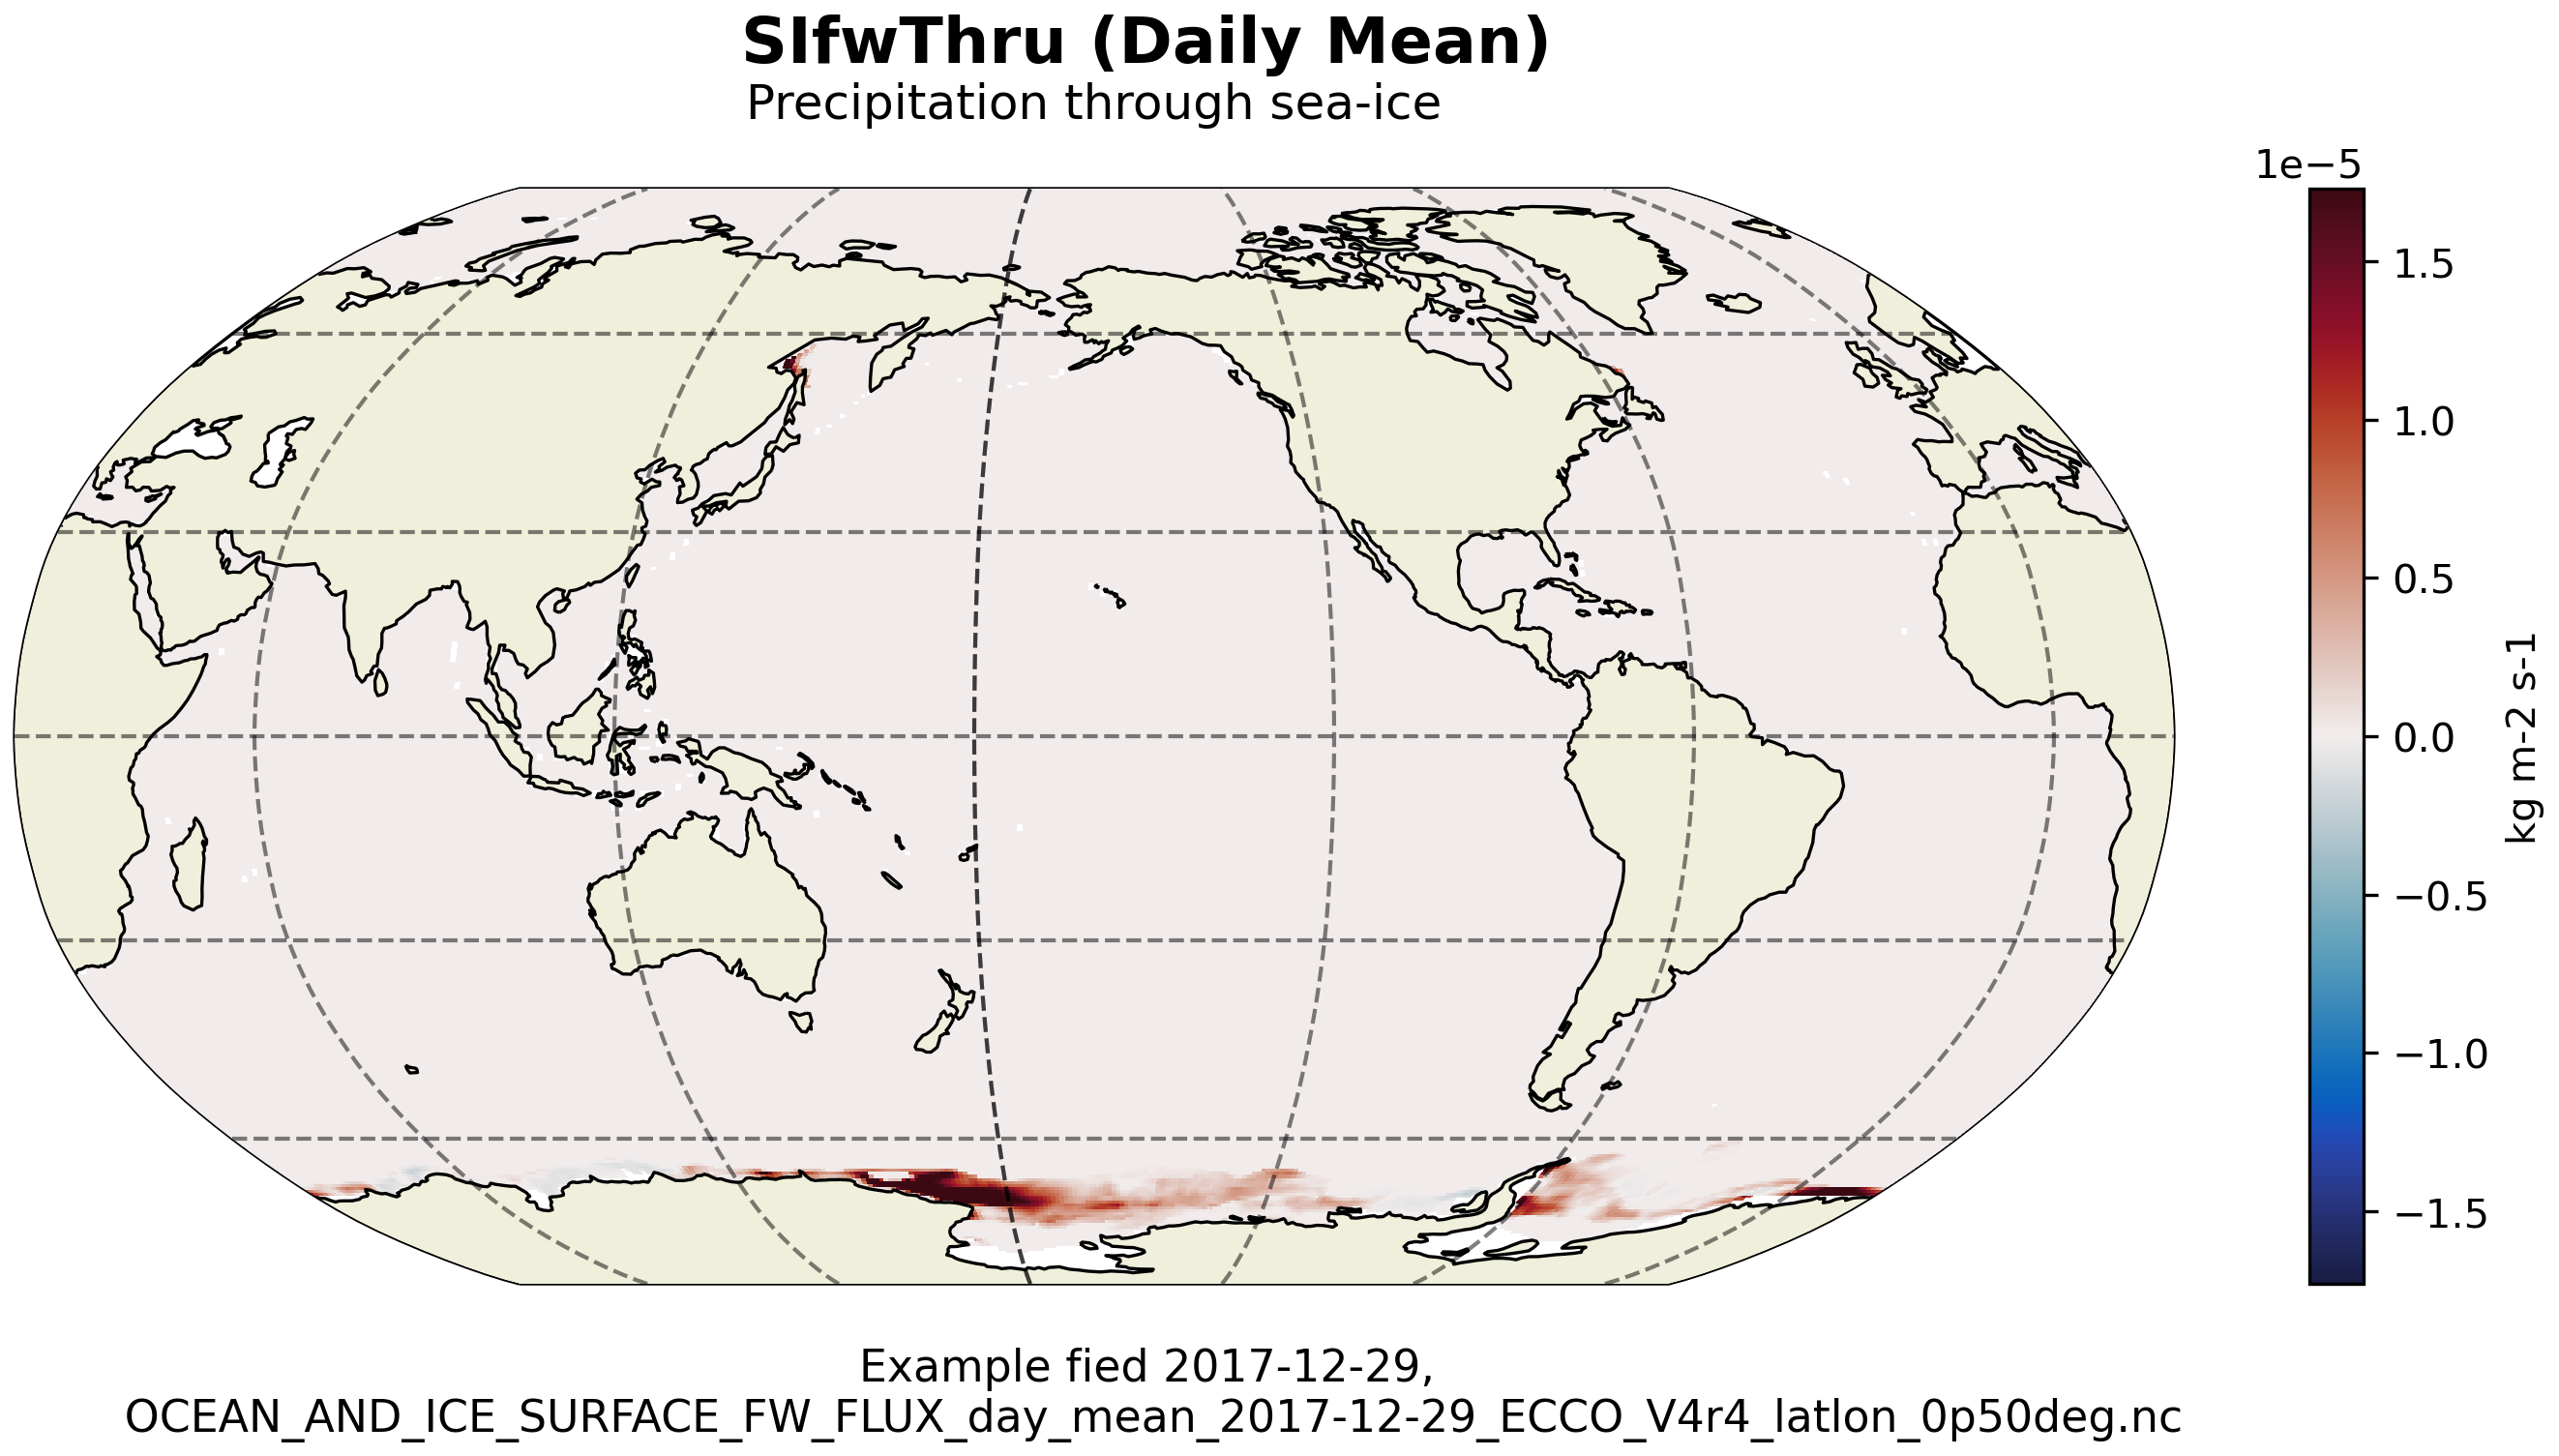
\includegraphics[width=\textwidth]{../images/plots/latlon_plots/Ocean_and_Sea-Ice_Surface_Freshwater_Fluxes/SIfwThru.png}
\caption{Dataset: OCEAN\_AND\_ICE\_SURFACE\_FW\_FLUX Variable: SIfwThru}
\label{tab:table-OCEAN_AND_ICE_SURFACE_FW_FLUX_SIfwThru-Plot}
\end{figure}
\pagebreak
\subsubsection{Latlon Variable SIrsSubl}
\begin{longtable}{|p{0.06\textwidth}|p{0.41\textwidth}|p{0.39\textwidth}|p{0.06\textwidth}|}
\caption{CDL description of OCEAN\_AND\_ICE\_SURFACE\_FW\_FLUX's SIrsSubl variable}
\label{tab:table-OCEAN_AND_ICE_SURFACE_FW_FLUX_SIrsSubl} \\ 
\hline \endhead \hline \endfoot
\rowcolor{lightgray} \textbf{Storage Type} & \textbf{Variable Name} & \textbf{Description} & \textbf{Unit} \\ \hline
float32 & SIrsSubl & Residual sublimation freshwater flux & kg m-2 s-1 \\ \hline
\rowcolor{lightgray}  \multicolumn{4}{|p{1.00\textwidth}|}{\textbf{CDL Description}} \\ \hline
\multicolumn{4}{|p{1.00\textwidth}|}{\makecell{\parbox{1\textwidth}{float32 SIrsSubl(time, latitude, longitude)\\
\hspace*{0.5cm}SIrsSubl: \_FillValue = 9.96921e+36\\
\hspace*{0.5cm}SIrsSubl: coverage\_content\_type = modelResult\\
\hspace*{0.5cm}SIrsSubl: direction = >0 decreases ocean volume\\
\hspace*{0.5cm}SIrsSubl: long\_name = Residual sublimation freshwater flux\\
\hspace*{0.5cm}SIrsSubl: units = kg m: 2 s: 1\\
\hspace*{0.5cm}SIrsSubl: coordinates = time\\
\hspace*{0.5cm}SIrsSubl: valid\_min = : 0.0001067528864950873\\
\hspace*{0.5cm}SIrsSubl: valid\_max = 8.640533451398369e: 06}}} \\ \hline
\rowcolor{lightgray} \multicolumn{4}{|p{1.00\textwidth}|}{\textbf{Comments}} \\ \hline
\multicolumn{4}{|p{1\textwidth}|}{Residual freshwater flux by sublimation to remove water from or add water to ocean. When implied sublimation freshwater flux SIacSubl is larger than availabe sea-ice/snow, SIrsSubl is positive and water is removed from ocean. Note: freshwater flux by sublimation that is to remove water from the ocean when it is positive.} \\ \hline
\end{longtable}

\begin{figure}[H]
\centering
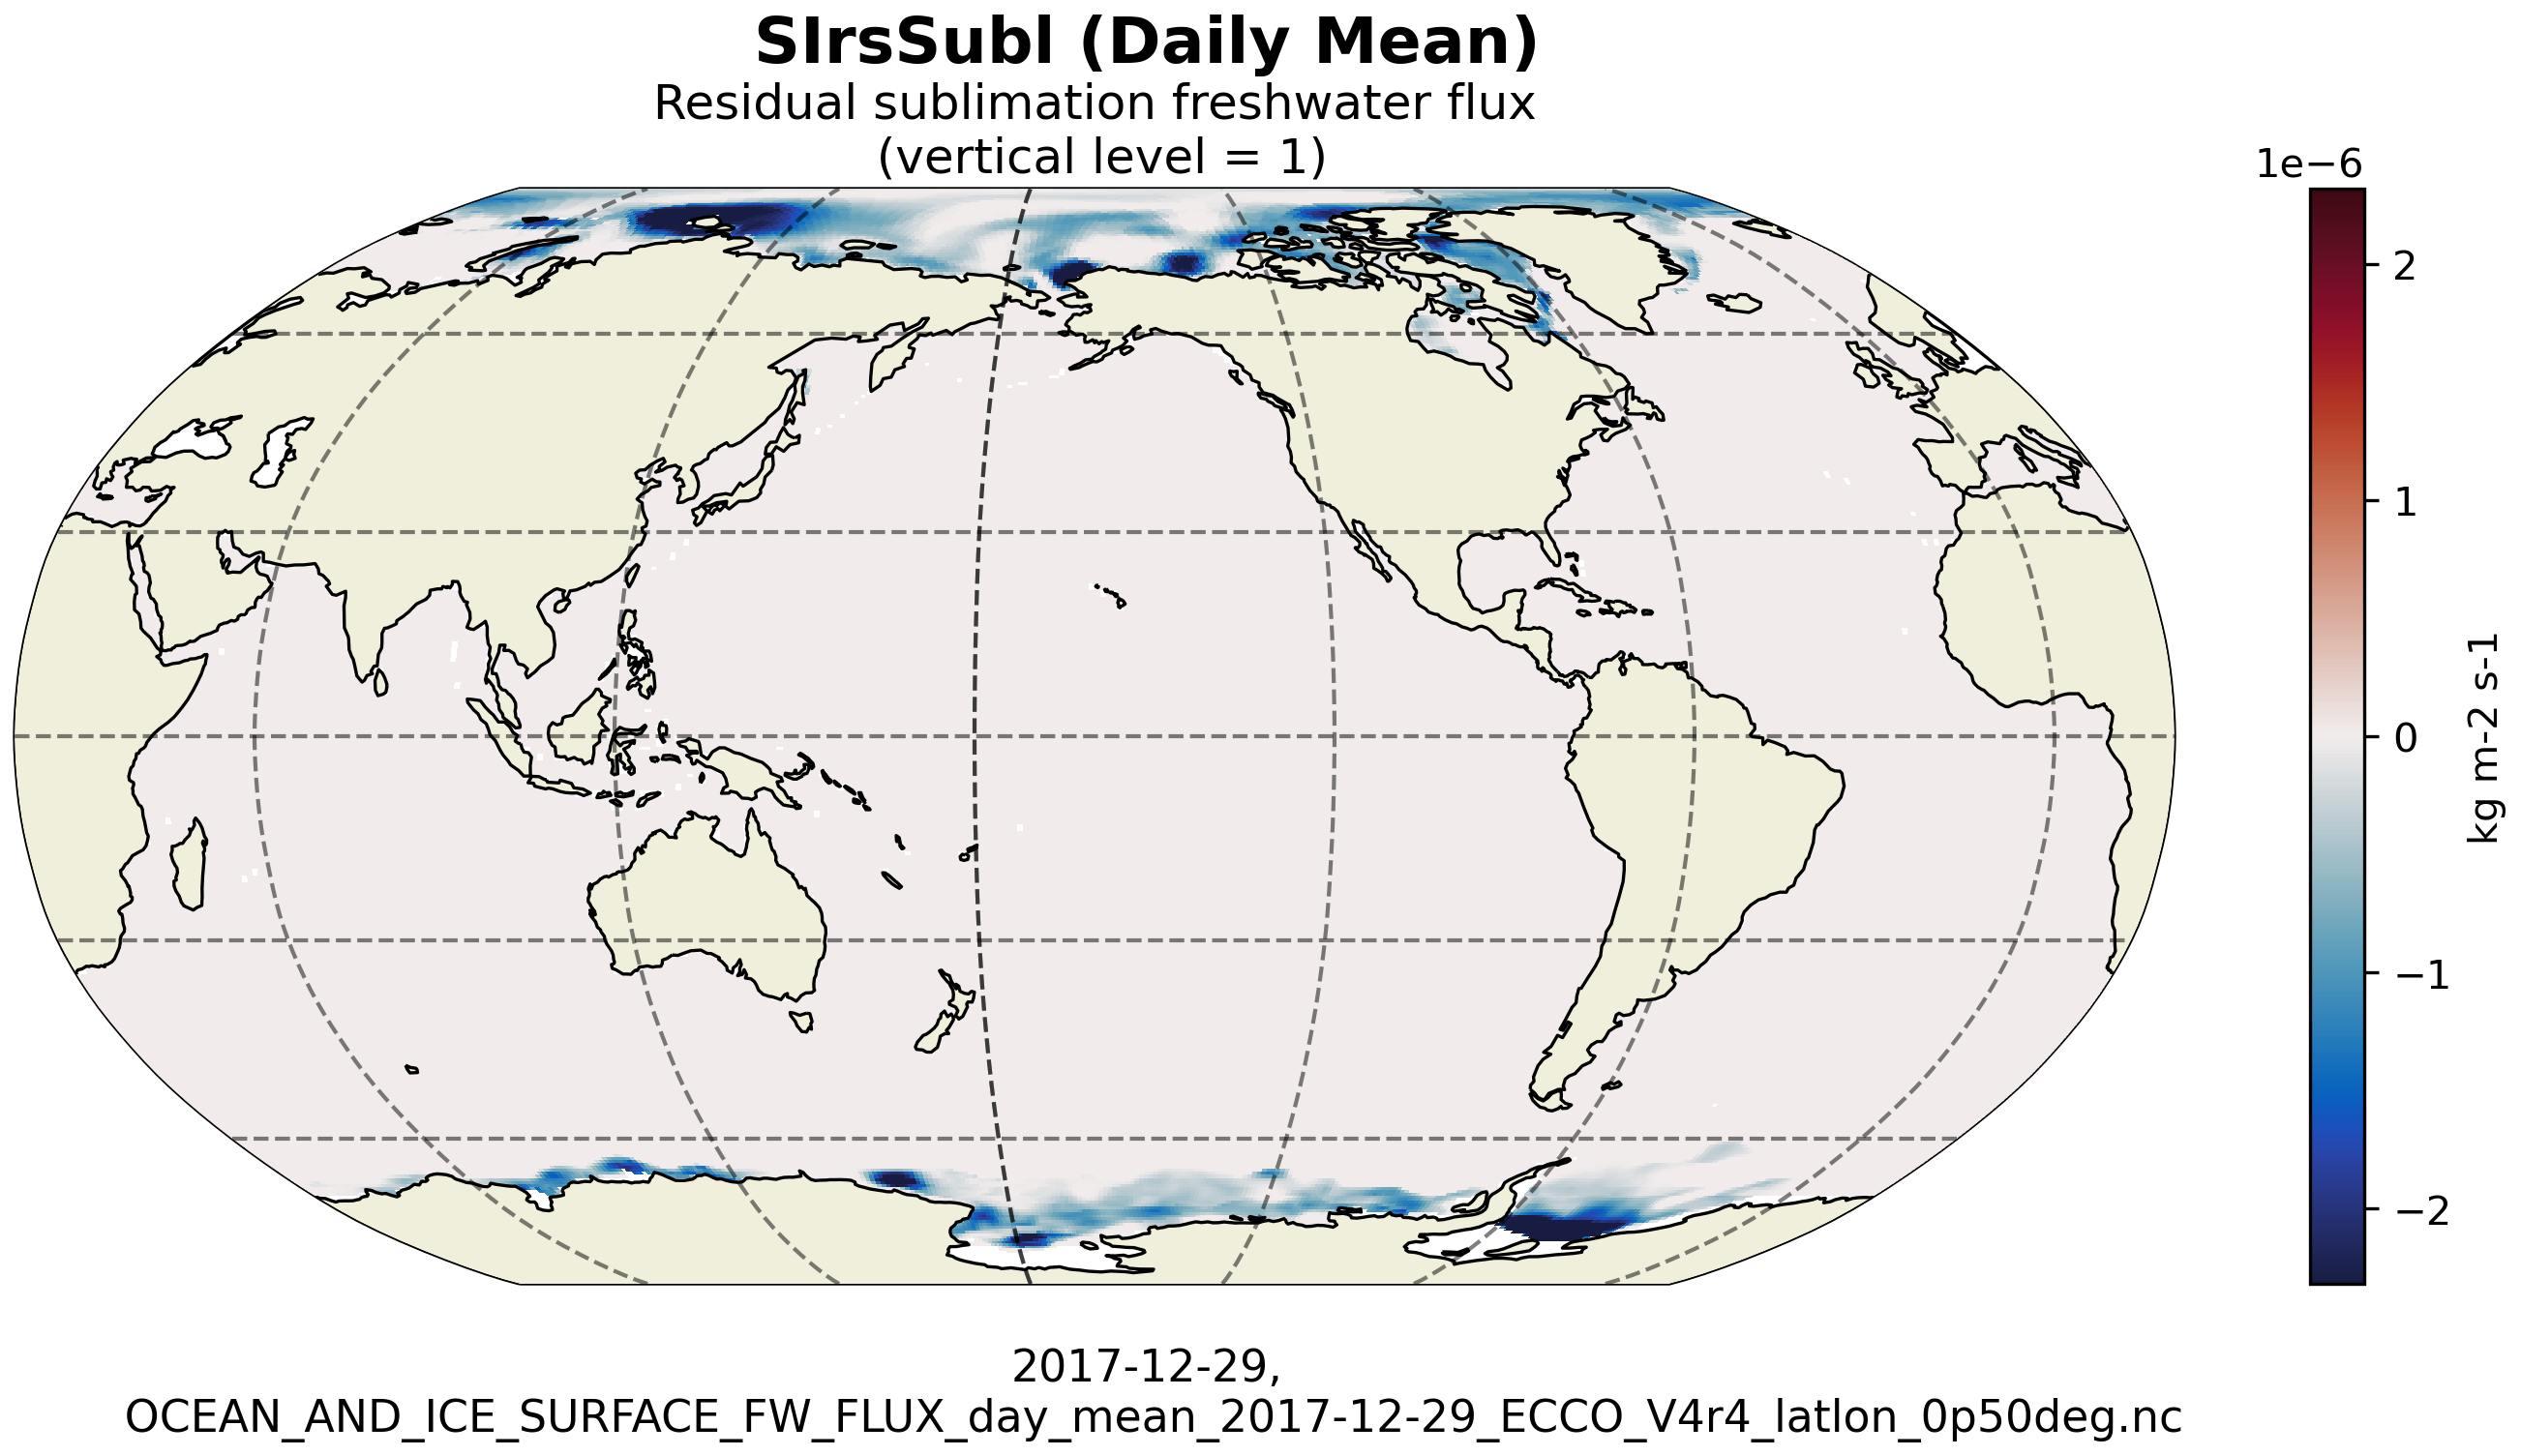
\includegraphics[width=\textwidth]{../images/plots/latlon_plots/Ocean_and_Sea-Ice_Surface_Freshwater_Fluxes/SIrsSubl.png}
\caption{Dataset: OCEAN\_AND\_ICE\_SURFACE\_FW\_FLUX Variable: SIrsSubl}
\label{tab:table-OCEAN_AND_ICE_SURFACE_FW_FLUX_SIrsSubl-Plot}
\end{figure}
\pagebreak
\subsubsection{Latlon Variable SIsnPrcp}
\begin{longtable}{|p{0.06\textwidth}|p{0.41\textwidth}|p{0.39\textwidth}|p{0.06\textwidth}|}
\caption{CDL description of OCEAN\_AND\_ICE\_SURFACE\_FW\_FLUX's SIsnPrcp variable}
\label{tab:table-OCEAN_AND_ICE_SURFACE_FW_FLUX_SIsnPrcp} \\ 
\hline \endhead \hline \endfoot
\rowcolor{lightgray} \textbf{Storage Type} & \textbf{Variable Name} & \textbf{Description} & \textbf{Unit} \\ \hline
float32 & SIsnPrcp & Snow precipitation on sea-ice & kg m-2 s-1 \\ \hline
\rowcolor{lightgray}  \multicolumn{4}{|p{1.00\textwidth}|}{\textbf{CDL Description}} \\ \hline
\multicolumn{4}{|p{1.00\textwidth}|}{\makecell{\parbox{1\textwidth}{float32 SIsnPrcp(time, latitude, longitude)\\
\hspace*{0.5cm}SIsnPrcp: \_FillValue = 9.96921e+36\\
\hspace*{0.5cm}SIsnPrcp: coverage\_content\_type = modelResult\\
\hspace*{0.5cm}SIsnPrcp: direction = >0 increases snow thickness (HSNOW)\\
\hspace*{0.5cm}SIsnPrcp: long\_name = Snow precipitation on sea: ice\\
\hspace*{0.5cm}SIsnPrcp: standard\_name = snowfall\_flux\\
\hspace*{0.5cm}SIsnPrcp: units = kg m: 2 s: 1\\
\hspace*{0.5cm}SIsnPrcp: coordinates = time\\
\hspace*{0.5cm}SIsnPrcp: valid\_min = : 4.334669574745931e: 05\\
\hspace*{0.5cm}SIsnPrcp: valid\_max = 0.0009354020585305989}}} \\ \hline
\rowcolor{lightgray} \multicolumn{4}{|p{1.00\textwidth}|}{\textbf{Comments}} \\ \hline
\multicolumn{4}{|p{1\textwidth}|}{Snow precipitation rate over sea-ice, averaged over the entire model grid cell.} \\ \hline
\end{longtable}

\begin{figure}[H]
\centering
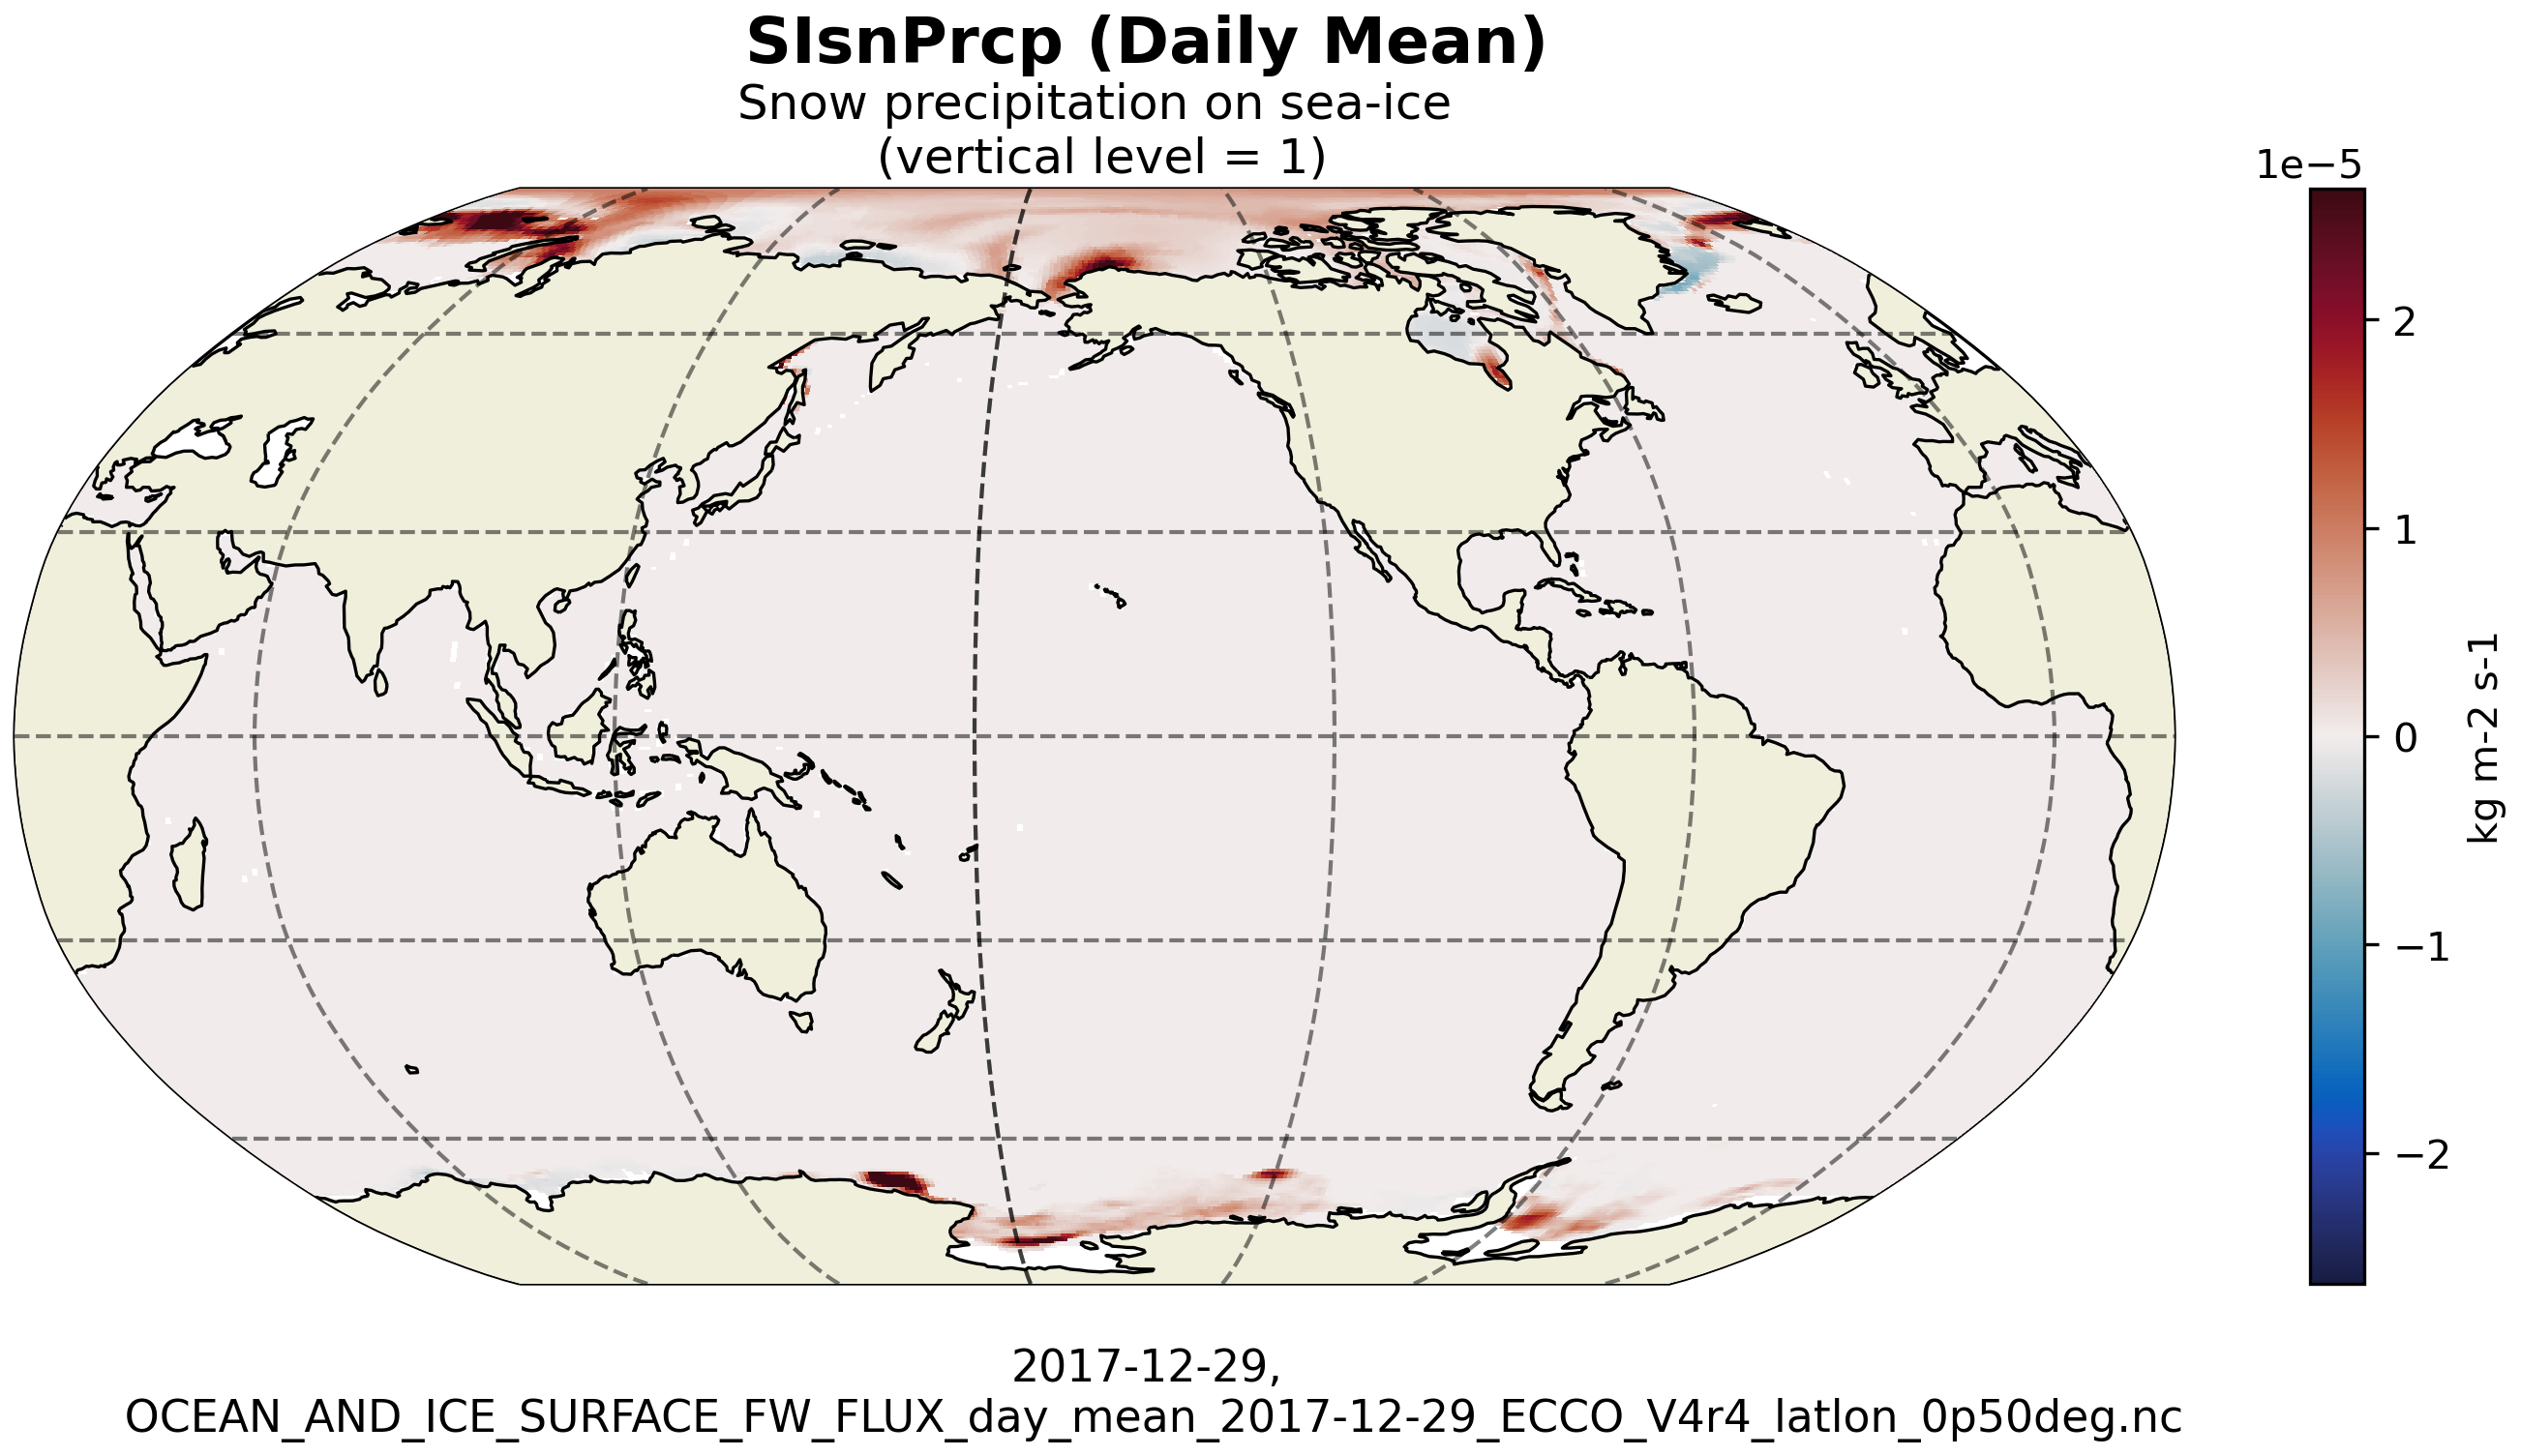
\includegraphics[width=\textwidth]{../images/plots/latlon_plots/Ocean_and_Sea-Ice_Surface_Freshwater_Fluxes/SIsnPrcp.png}
\caption{Dataset: OCEAN\_AND\_ICE\_SURFACE\_FW\_FLUX Variable: SIsnPrcp}
\label{tab:table-OCEAN_AND_ICE_SURFACE_FW_FLUX_SIsnPrcp-Plot}
\end{figure}
\pagebreak
\subsubsection{Latlon Variable oceFWflx}
\begin{longtable}{|p{0.06\textwidth}|p{0.41\textwidth}|p{0.39\textwidth}|p{0.06\textwidth}|}
\caption{CDL description of OCEAN\_AND\_ICE\_SURFACE\_FW\_FLUX's oceFWflx variable}
\label{tab:table-OCEAN_AND_ICE_SURFACE_FW_FLUX_oceFWflx} \\ 
\hline \endhead \hline \endfoot
\rowcolor{lightgray} \textbf{Storage Type} & \textbf{Variable Name} & \textbf{Description} & \textbf{Unit} \\ \hline
float32 & oceFWflx & Net freshwater flux into the ocean & kg m-2 s-1 \\ \hline
\rowcolor{lightgray}  \multicolumn{4}{|p{1.00\textwidth}|}{\textbf{CDL Description}} \\ \hline
\multicolumn{4}{|p{1.00\textwidth}|}{\makecell{\parbox{1\textwidth}{float32 oceFWflx(time, latitude, longitude)\\
\hspace*{0.5cm}oceFWflx: \_FillValue = 9.96921e+36\\
\hspace*{0.5cm}oceFWflx: coverage\_content\_type = modelResult\\
\hspace*{0.5cm}oceFWflx: direction = >0 decreases salinity (SALT)\\
\hspace*{0.5cm}oceFWflx: long\_name = Net freshwater flux into the ocean\\
\hspace*{0.5cm}oceFWflx: standard\_name = water\_flux\_into\_sea\_water\\
\hspace*{0.5cm}oceFWflx: units = kg m: 2 s: 1\\
\hspace*{0.5cm}oceFWflx: coordinates = time\\
\hspace*{0.5cm}oceFWflx: valid\_min = : 0.0033125500194728374\\
\hspace*{0.5cm}oceFWflx: valid\_max = 0.008299433626234531}}} \\ \hline
\rowcolor{lightgray} \multicolumn{4}{|p{1.00\textwidth}|}{\textbf{Comments}} \\ \hline
\multicolumn{4}{|p{1\textwidth}|}{Net freshwater flux into the ocean including contributions from runoff, evaporation, precipitation, and mass exchange with sea-ice due to melting and freezing and snow melting. Note: oceFWflx does NOT include freshwater fluxes between the atmosphere and sea-ice and snow. The variable 'SIatmFW' accounts for freshwater fluxes out of the combined ocean+sea-ice+snow reservoir.} \\ \hline
\end{longtable}

\begin{figure}[H]
\centering
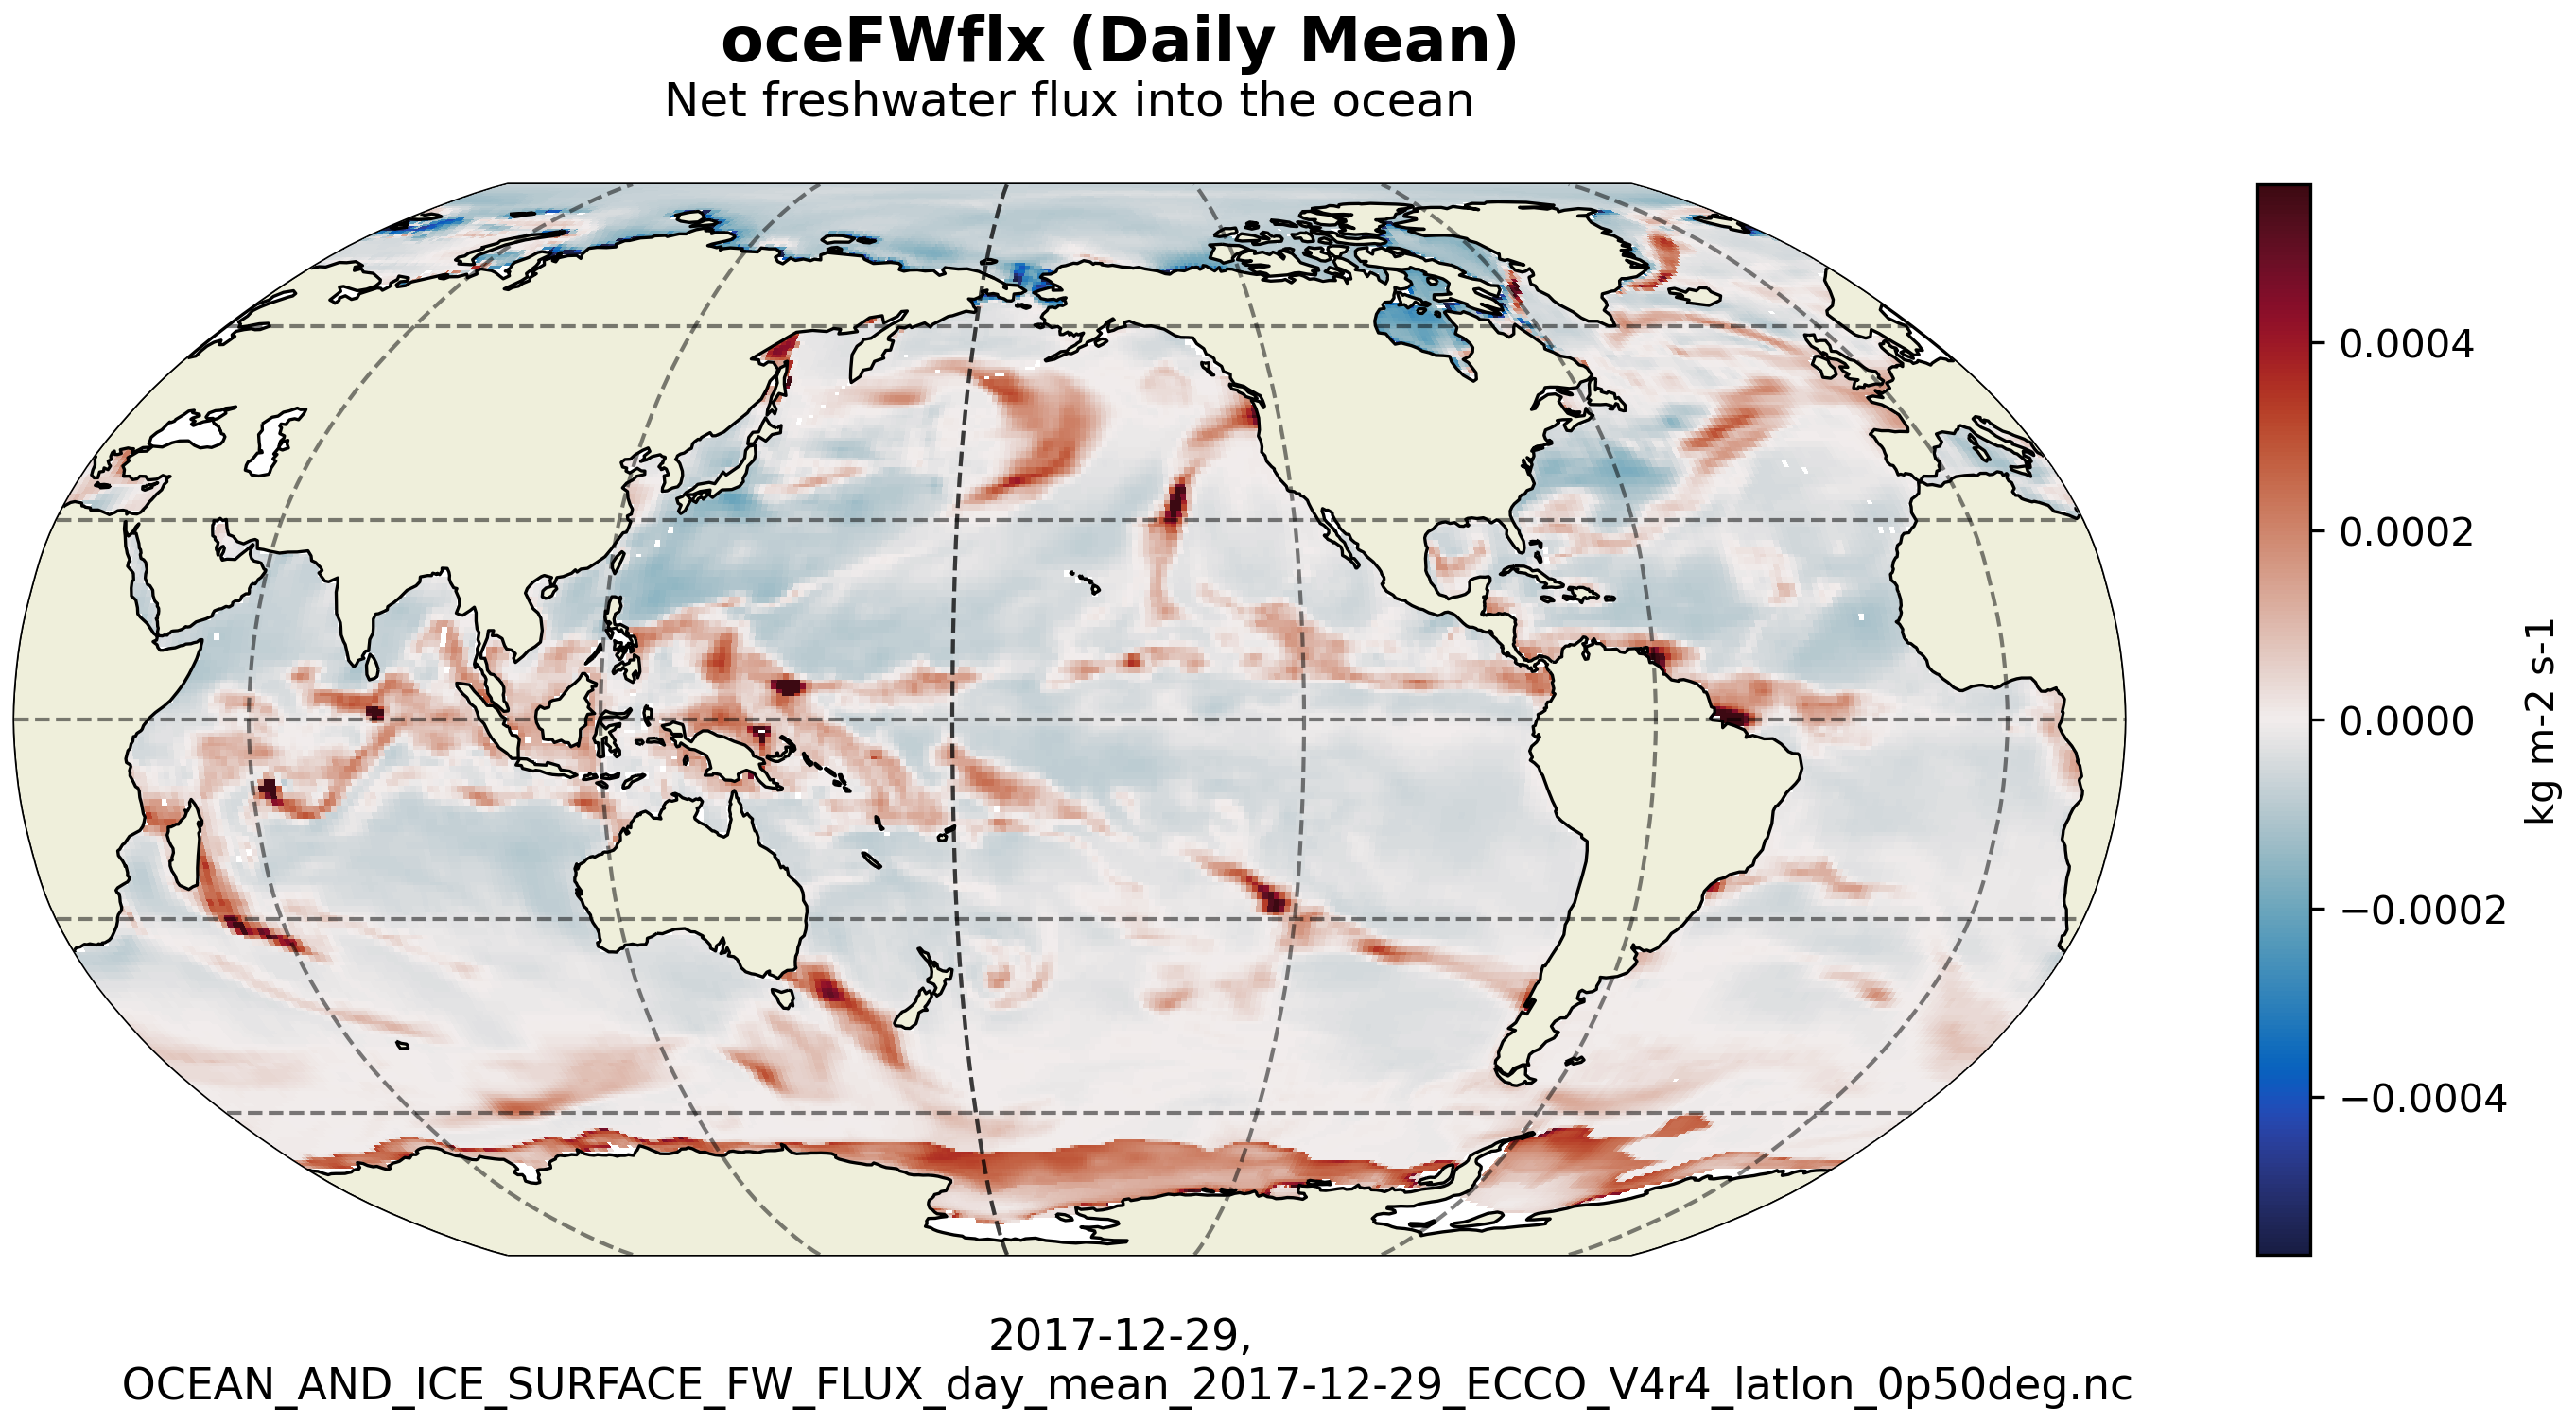
\includegraphics[width=\textwidth]{../images/plots/latlon_plots/Ocean_and_Sea-Ice_Surface_Freshwater_Fluxes/oceFWflx.png}
\caption{Dataset: OCEAN\_AND\_ICE\_SURFACE\_FW\_FLUX Variable: oceFWflx}
\label{tab:table-OCEAN_AND_ICE_SURFACE_FW_FLUX_oceFWflx-Plot}
\end{figure}
\pagebreak
\subsection{Latlon NetCDF OCEAN\_AND\_ICE\_SURFACE\_HEAT\_FLUX}
\newp
\begin{longtable}{|p{0.1\textwidth}|p{0.5\textwidth}|}
\caption{Variables in the dataset OCEAN\_AND\_ICE\_SURFACE\_HEAT\_FLUX}
\label{tab:table-OCEAN_AND_ICE_SURFACE_HEAT_FLUX-fields} \\ 
\hline \endhead \hline \endfoot
\rowcolor{lightgray} \textbf{Dataset:} & \textbf{OCEAN\_AND\_ICE\_SURFACE\_HEAT\_FLUX} \\ \hline
Field: &EXFhl \\ \hline
Field: &EXFhs \\ \hline
Field: &EXFlwdn \\ \hline
Field: &EXFswdn \\ \hline
Field: &EXFqnet \\ \hline
Field: &oceQnet \\ \hline
Field: &SIatmQnt \\ \hline
Field: &TFLUX \\ \hline
Field: &EXFswnet \\ \hline
Field: &EXFlwnet \\ \hline
Field: &oceQsw \\ \hline
Field: &SIaaflux \\ \hline
\end{longtable}

\pagebreak
\subsubsection{Latlon Variable EXFhl}
\begin{longtable}{|p{0.06\textwidth}|p{0.41\textwidth}|p{0.39\textwidth}|p{0.06\textwidth}|}
\caption{CDL description of OCEAN\_AND\_ICE\_SURFACE\_HEAT\_FLUX's EXFhl variable}
\label{tab:table-OCEAN_AND_ICE_SURFACE_HEAT_FLUX_EXFhl} \\ 
\hline \endhead \hline \endfoot
\rowcolor{lightgray} \textbf{Storage Type} & \textbf{Variable Name} & \textbf{Description} & \textbf{Unit} \\ \hline
float32 & EXFhl & Open ocean air-sea latent heat flux & W m-2 \\ \hline
\rowcolor{lightgray}  \multicolumn{4}{|p{1.00\textwidth}|}{\textbf{CDL Description}} \\ \hline
\multicolumn{4}{|p{1.00\textwidth}|}{\makecell{\parbox{1\textwidth}{float32 EXFhl(time, latitude, longitude)\\
\hspace*{0.5cm}EXFhl: \_FillValue = 9.96921e+36\\
\hspace*{0.5cm}EXFhl: coverage\_content\_type = modelResult\\
\hspace*{0.5cm}EXFhl: direction = >0 increases potential temperature (THETA)\\
\hspace*{0.5cm}EXFhl: long\_name = Open ocean air: sea latent heat flux\\
\hspace*{0.5cm}EXFhl: standard\_name = surface\_downward\_latent\_heat\_flux\\
\hspace*{0.5cm}EXFhl: units = W m: 2\\
\hspace*{0.5cm}EXFhl: coordinates = time\\
\hspace*{0.5cm}EXFhl: valid\_min = : 1772.513671875\\
\hspace*{0.5cm}EXFhl: valid\_max = 273.9528503417969}}} \\ \hline
\rowcolor{lightgray} \multicolumn{4}{|p{1.00\textwidth}|}{\textbf{Comments}} \\ \hline
\multicolumn{4}{|p{1\textwidth}|}{Air-sea latent heat flux per unit area of open water (not covered by sea-ice). Note: calculated from the bulk formula following Large and Yeager (2004) NCAR/TN-460+STR.} \\ \hline
\end{longtable}

\begin{figure}[H]
\centering
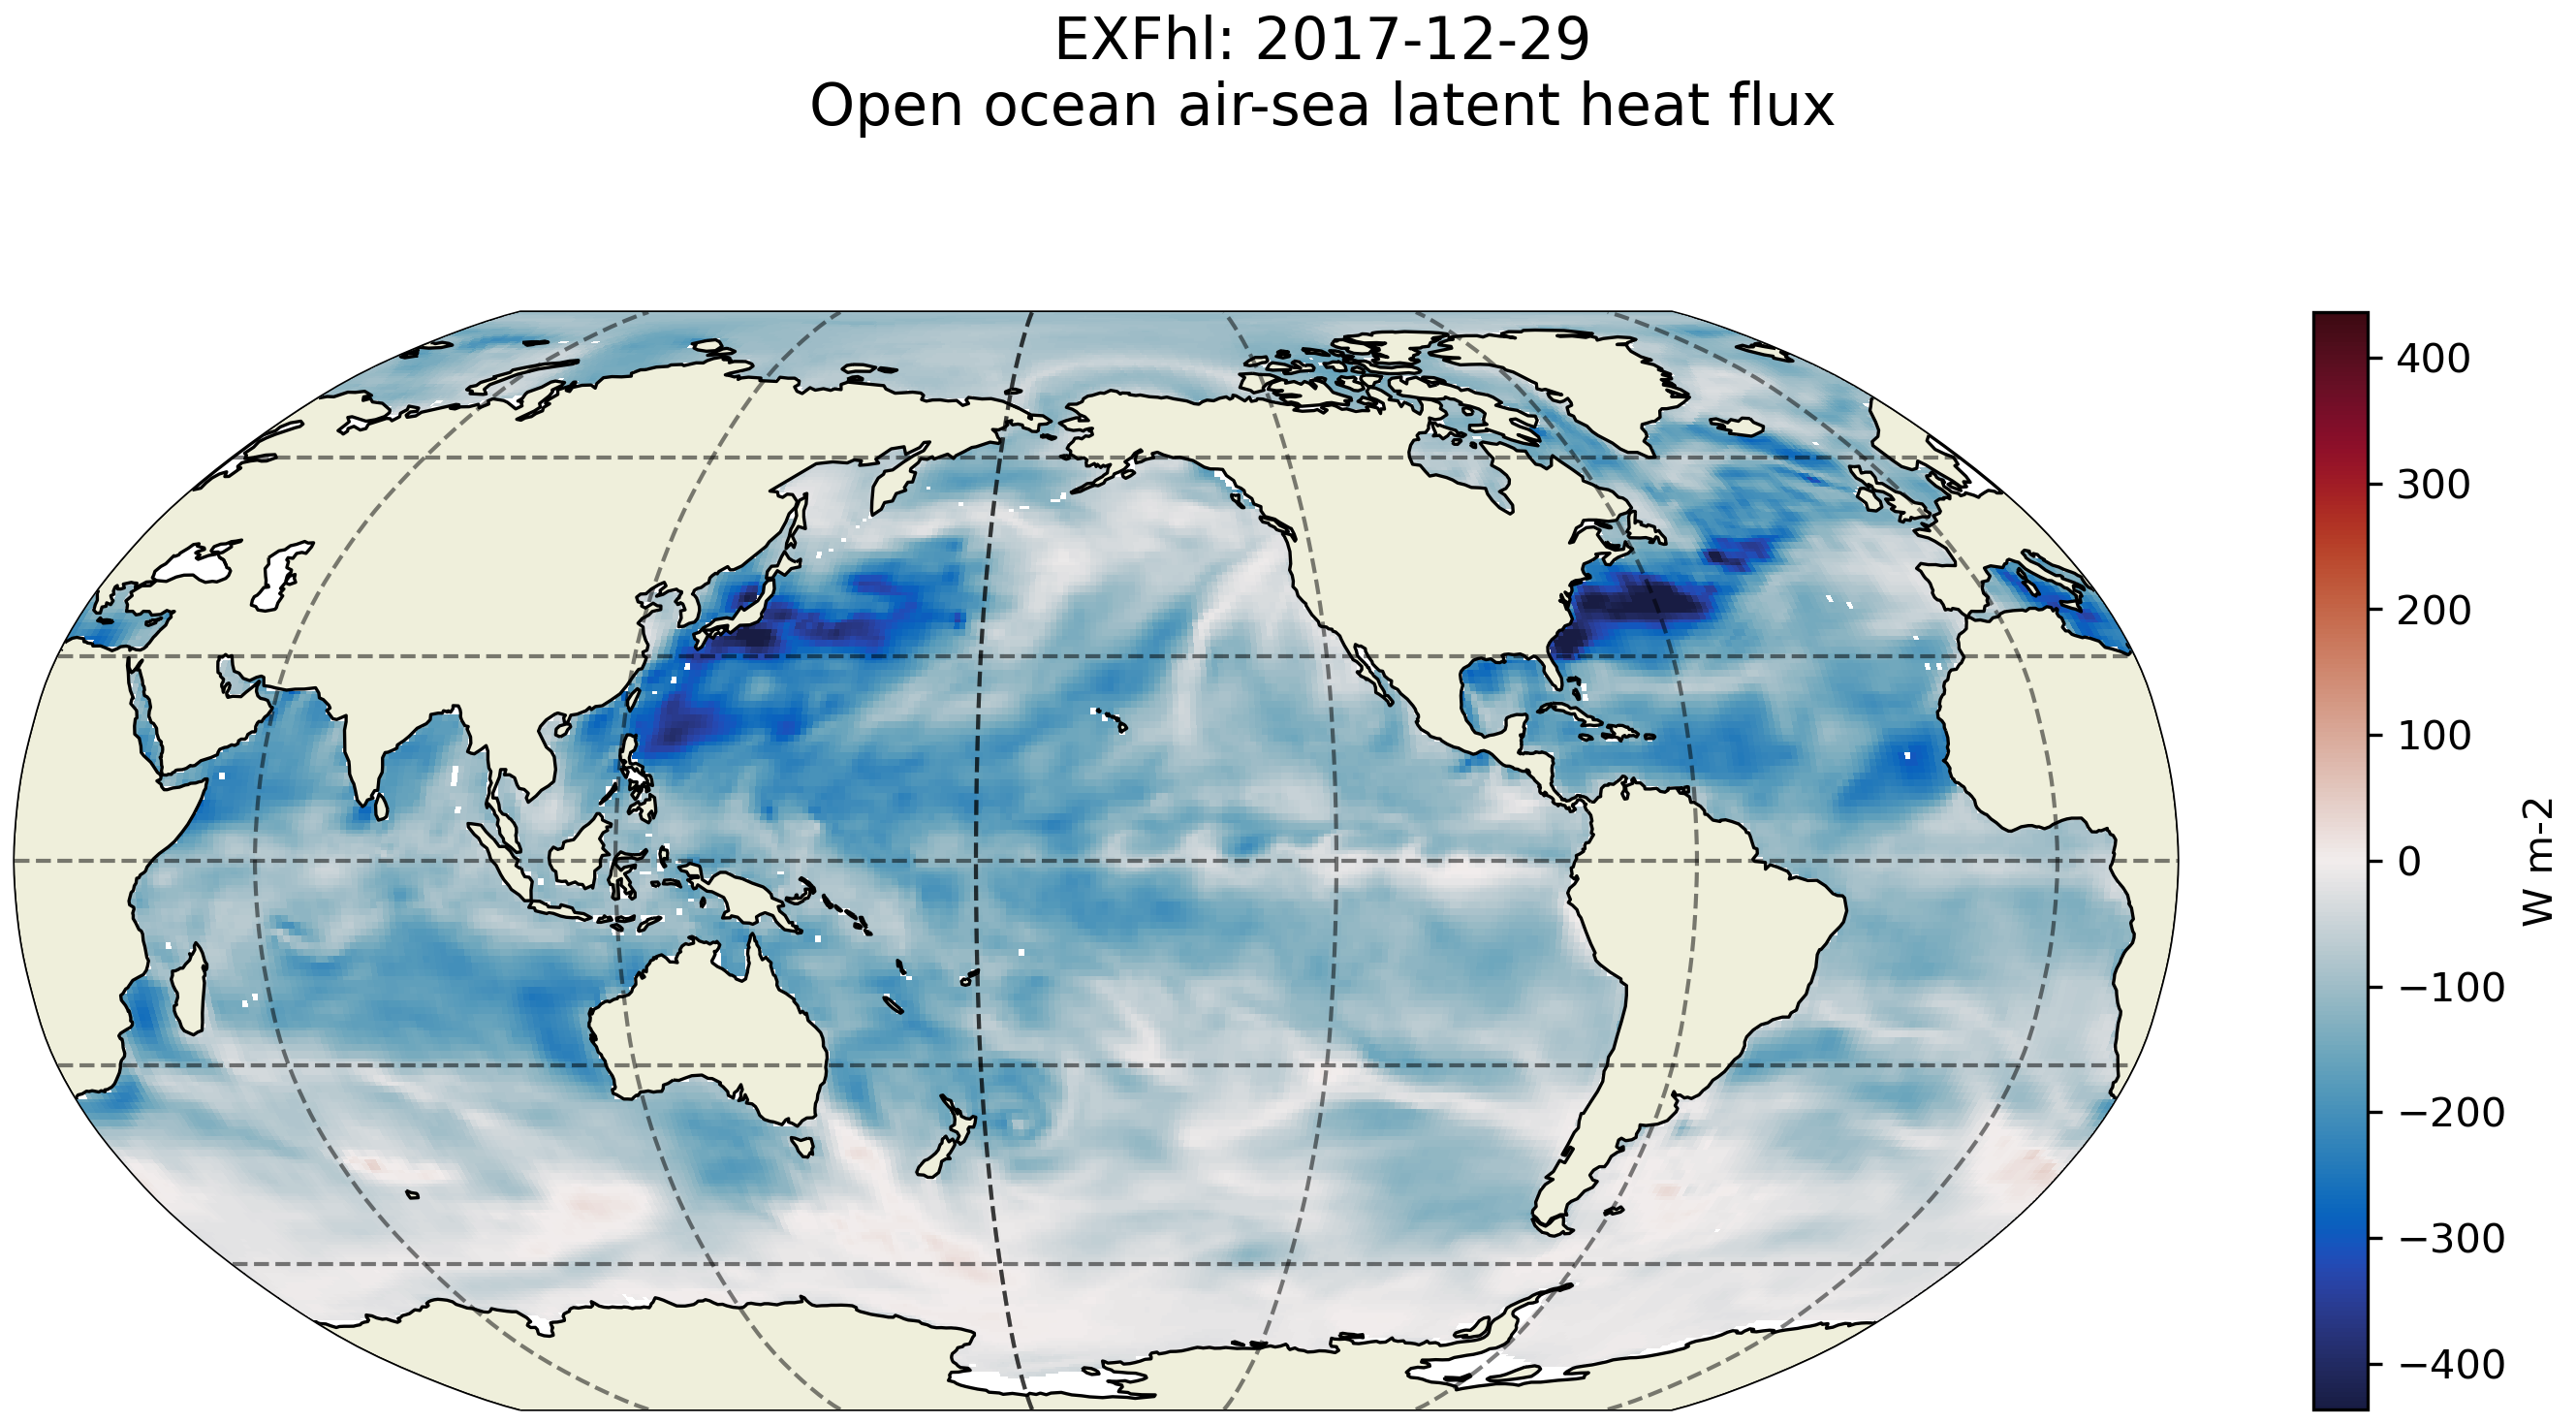
\includegraphics[width=\textwidth]{../images/plots/latlon_plots/Ocean_and_Sea-Ice_Surface_Heat_Fluxes/EXFhl.png}
\caption{Dataset: OCEAN\_AND\_ICE\_SURFACE\_HEAT\_FLUX Variable: EXFhl}
\label{tab:table-OCEAN_AND_ICE_SURFACE_HEAT_FLUX_EXFhl-Plot}
\end{figure}
\pagebreak
\subsubsection{Latlon Variable EXFhs}
\begin{longtable}{|p{0.06\textwidth}|p{0.41\textwidth}|p{0.39\textwidth}|p{0.06\textwidth}|}
\caption{CDL description of OCEAN\_AND\_ICE\_SURFACE\_HEAT\_FLUX's EXFhs variable}
\label{tab:table-OCEAN_AND_ICE_SURFACE_HEAT_FLUX_EXFhs} \\ 
\hline \endhead \hline \endfoot
\rowcolor{lightgray} \textbf{Storage Type} & \textbf{Variable Name} & \textbf{Description} & \textbf{Unit} \\ \hline
float32 & EXFhs & Open ocean air-sea sensible heat flux & W m-2 \\ \hline
\rowcolor{lightgray}  \multicolumn{4}{|p{1.00\textwidth}|}{\textbf{CDL Description}} \\ \hline
\multicolumn{4}{|p{1.00\textwidth}|}{\makecell{\parbox{1\textwidth}{float32 EXFhs(time, latitude, longitude)\\
\hspace*{0.5cm}EXFhs: \_FillValue = 9.96921e+36\\
\hspace*{0.5cm}EXFhs: coverage\_content\_type = modelResult\\
\hspace*{0.5cm}EXFhs: direction = >0 increases potential temperature (THETA)\\
\hspace*{0.5cm}EXFhs: long\_name = Open ocean air: sea sensible heat flux\\
\hspace*{0.5cm}EXFhs: standard\_name = surface\_downward\_sensible\_heat\_flux\\
\hspace*{0.5cm}EXFhs: units = W m: 2\\
\hspace*{0.5cm}EXFhs: coordinates = time\\
\hspace*{0.5cm}EXFhs: valid\_min = : 2478.766357421875\\
\hspace*{0.5cm}EXFhs: valid\_max = 357.0105895996094}}} \\ \hline
\rowcolor{lightgray} \multicolumn{4}{|p{1.00\textwidth}|}{\textbf{Comments}} \\ \hline
\multicolumn{4}{|p{1\textwidth}|}{Air-sea sensible heat flux per unit area of open water (not covered by sea-ice). Note: calculated from the bulk formula following Large and Yeager (2004) NCAR/TN-460+STR.} \\ \hline
\end{longtable}

\begin{figure}[H]
\centering
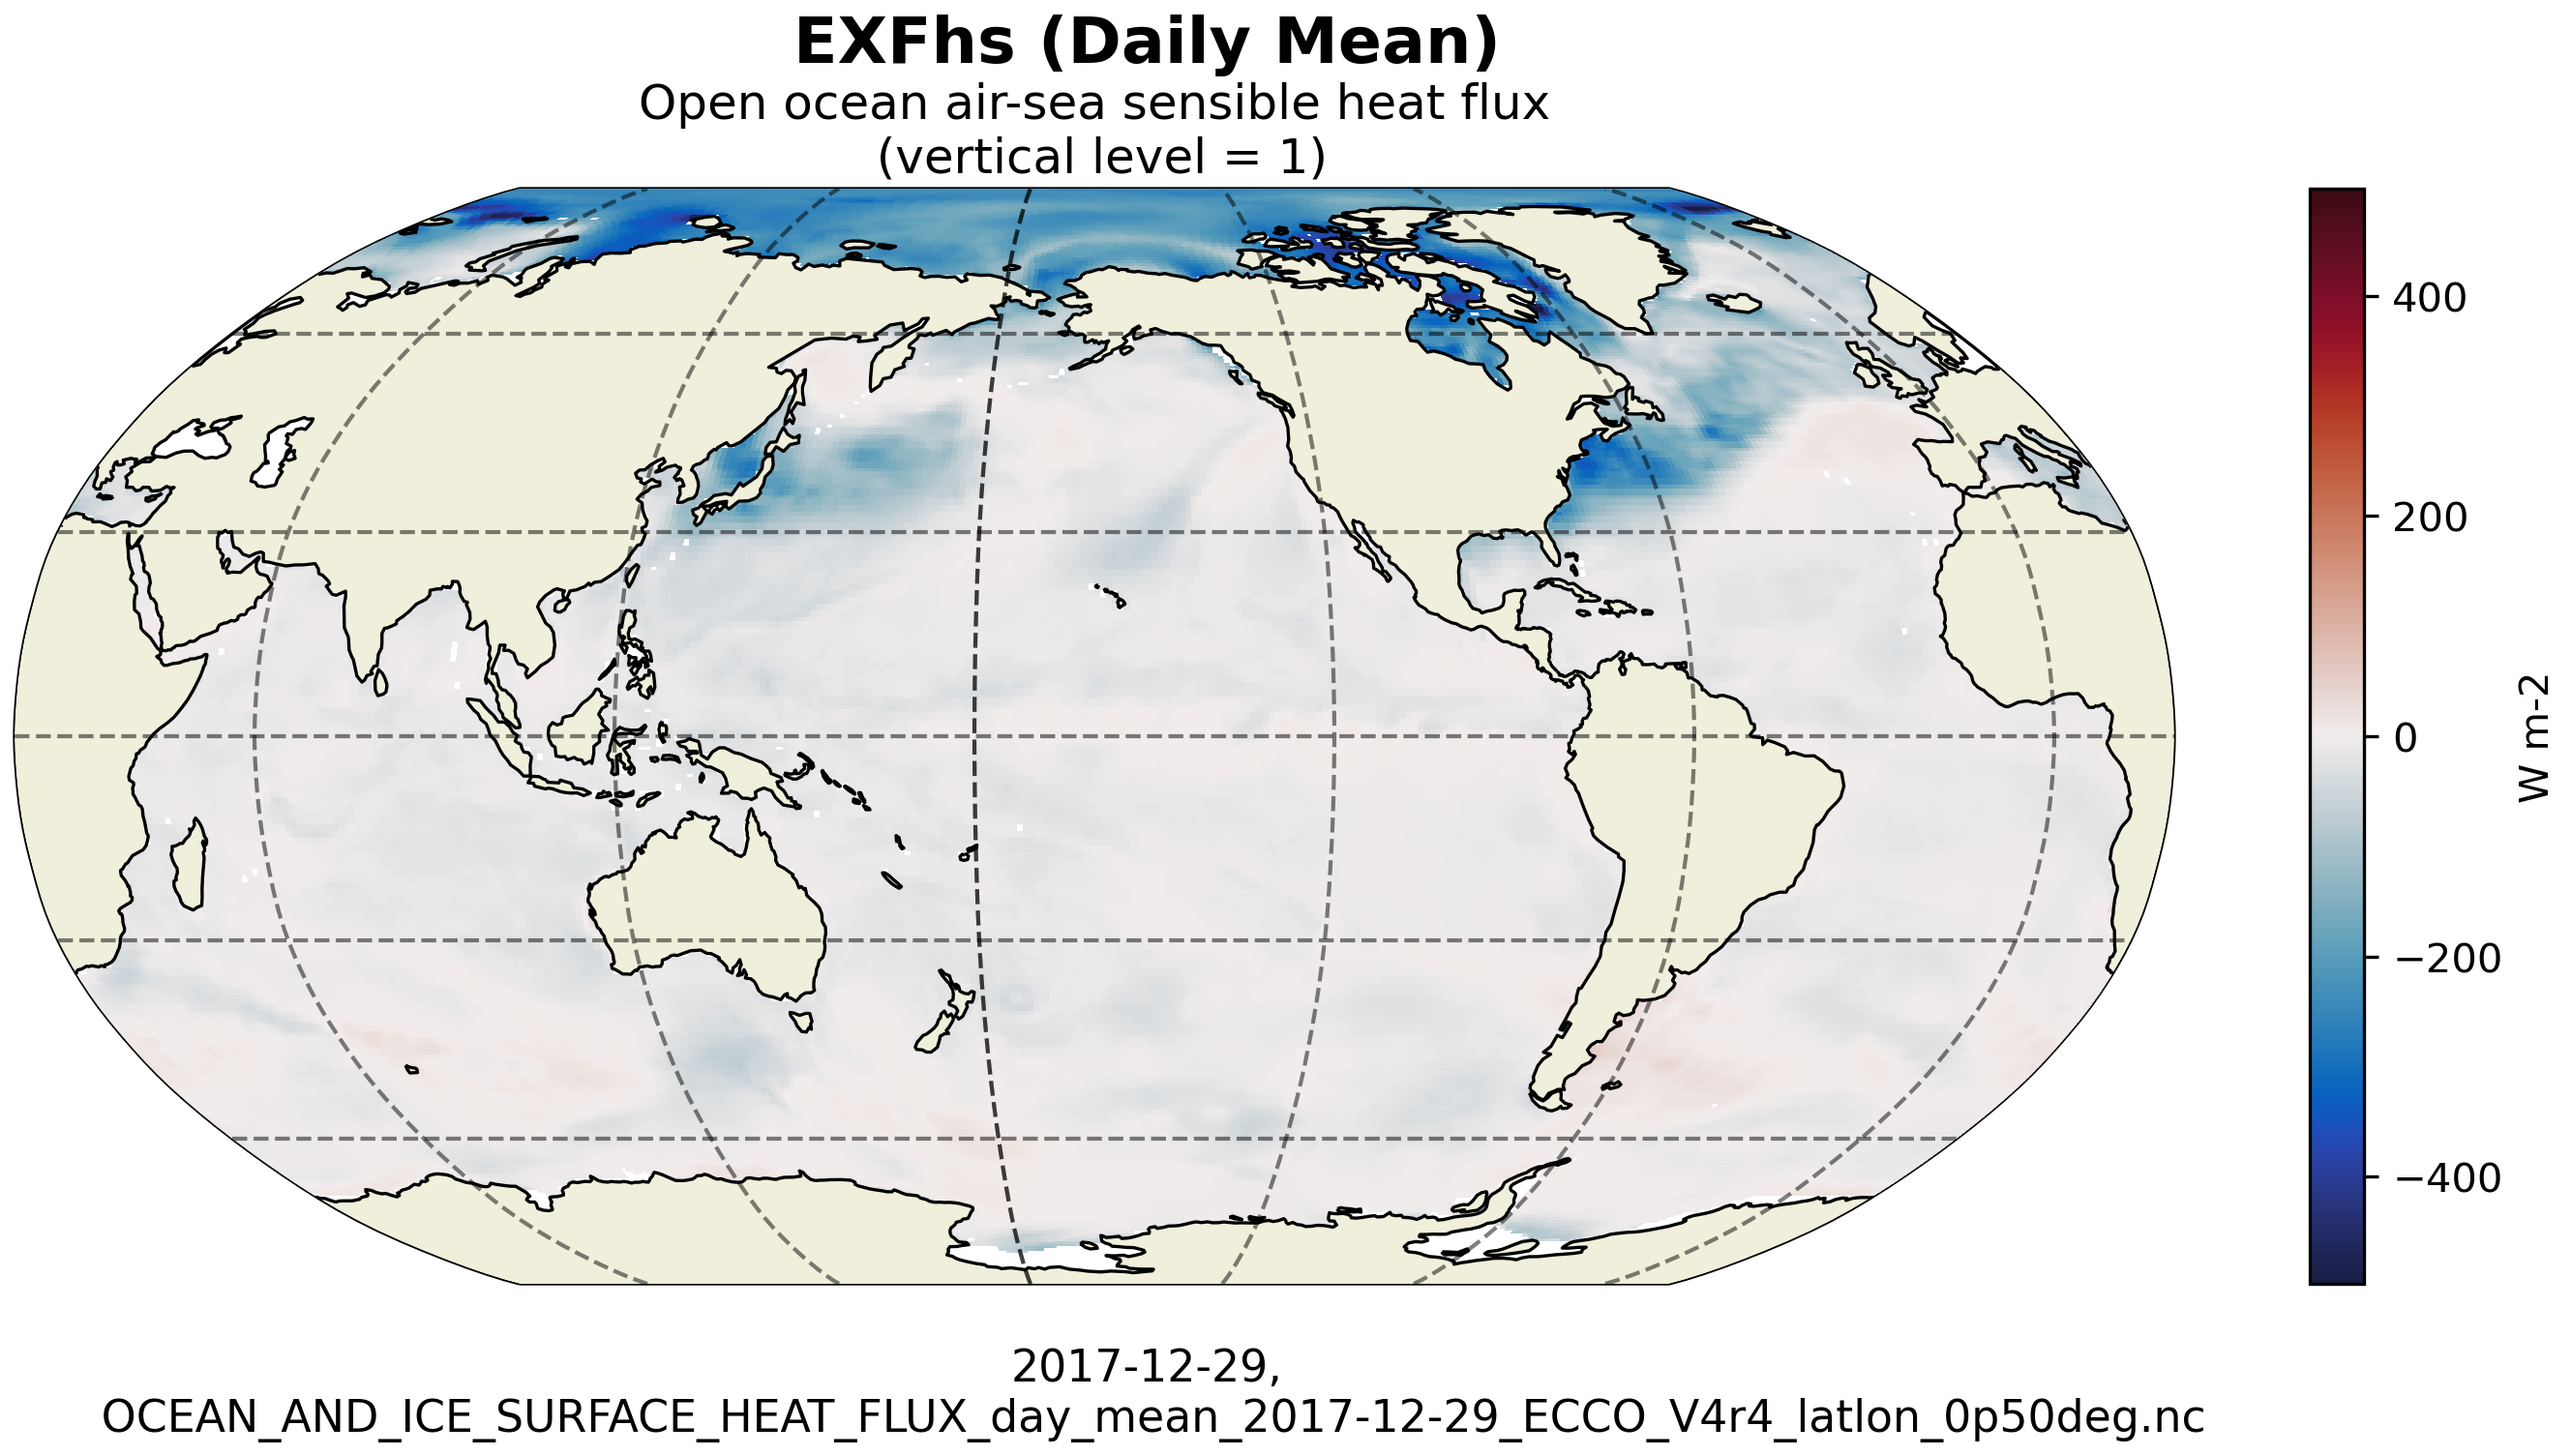
\includegraphics[width=\textwidth]{../images/plots/latlon_plots/Ocean_and_Sea-Ice_Surface_Heat_Fluxes/EXFhs.png}
\caption{Dataset: OCEAN\_AND\_ICE\_SURFACE\_HEAT\_FLUX Variable: EXFhs}
\label{tab:table-OCEAN_AND_ICE_SURFACE_HEAT_FLUX_EXFhs-Plot}
\end{figure}
\pagebreak
\subsubsection{Latlon Variable EXFlwdn}
\begin{longtable}{|p{0.06\textwidth}|p{0.41\textwidth}|p{0.39\textwidth}|p{0.06\textwidth}|}
\caption{CDL description of OCEAN\_AND\_ICE\_SURFACE\_HEAT\_FLUX's EXFlwdn variable}
\label{tab:table-OCEAN_AND_ICE_SURFACE_HEAT_FLUX_EXFlwdn} \\ 
\hline \endhead \hline \endfoot
\rowcolor{lightgray} \textbf{Storage Type} & \textbf{Variable Name} & \textbf{Description} & \textbf{Unit} \\ \hline
float32 & EXFlwdn & Downward longwave radiative flux & W m-2 \\ \hline
\rowcolor{lightgray}  \multicolumn{4}{|p{1.00\textwidth}|}{\textbf{CDL Description}} \\ \hline
\multicolumn{4}{|p{1.00\textwidth}|}{\makecell{\parbox{1\textwidth}{float32 EXFlwdn(time, latitude, longitude)\\
\hspace*{0.5cm}EXFlwdn: \_FillValue = 9.96921e+36\\
\hspace*{0.5cm}EXFlwdn: coverage\_content\_type = modelResult\\
\hspace*{0.5cm}EXFlwdn: direction = >0 increases potential temperature (THETA)\\
\hspace*{0.5cm}EXFlwdn: long\_name = Downward longwave radiative flux\\
\hspace*{0.5cm}EXFlwdn: standard\_name = surface\_downwelling\_longwave\_flux\_in\_air\\
\hspace*{0.5cm}EXFlwdn: units = W m: 2\\
\hspace*{0.5cm}EXFlwdn: coordinates = time\\
\hspace*{0.5cm}EXFlwdn: valid\_min = 4.188045501708984\\
\hspace*{0.5cm}EXFlwdn: valid\_max = 513.3919067382812}}} \\ \hline
\rowcolor{lightgray} \multicolumn{4}{|p{1.00\textwidth}|}{\textbf{Comments}} \\ \hline
\multicolumn{4}{|p{1\textwidth}|}{Downward longwave radiative flux. Note: sum of ERA-Interim downward longwave radiation and the control adjustment from ocean state estimation.} \\ \hline
\end{longtable}

\begin{figure}[H]
\centering
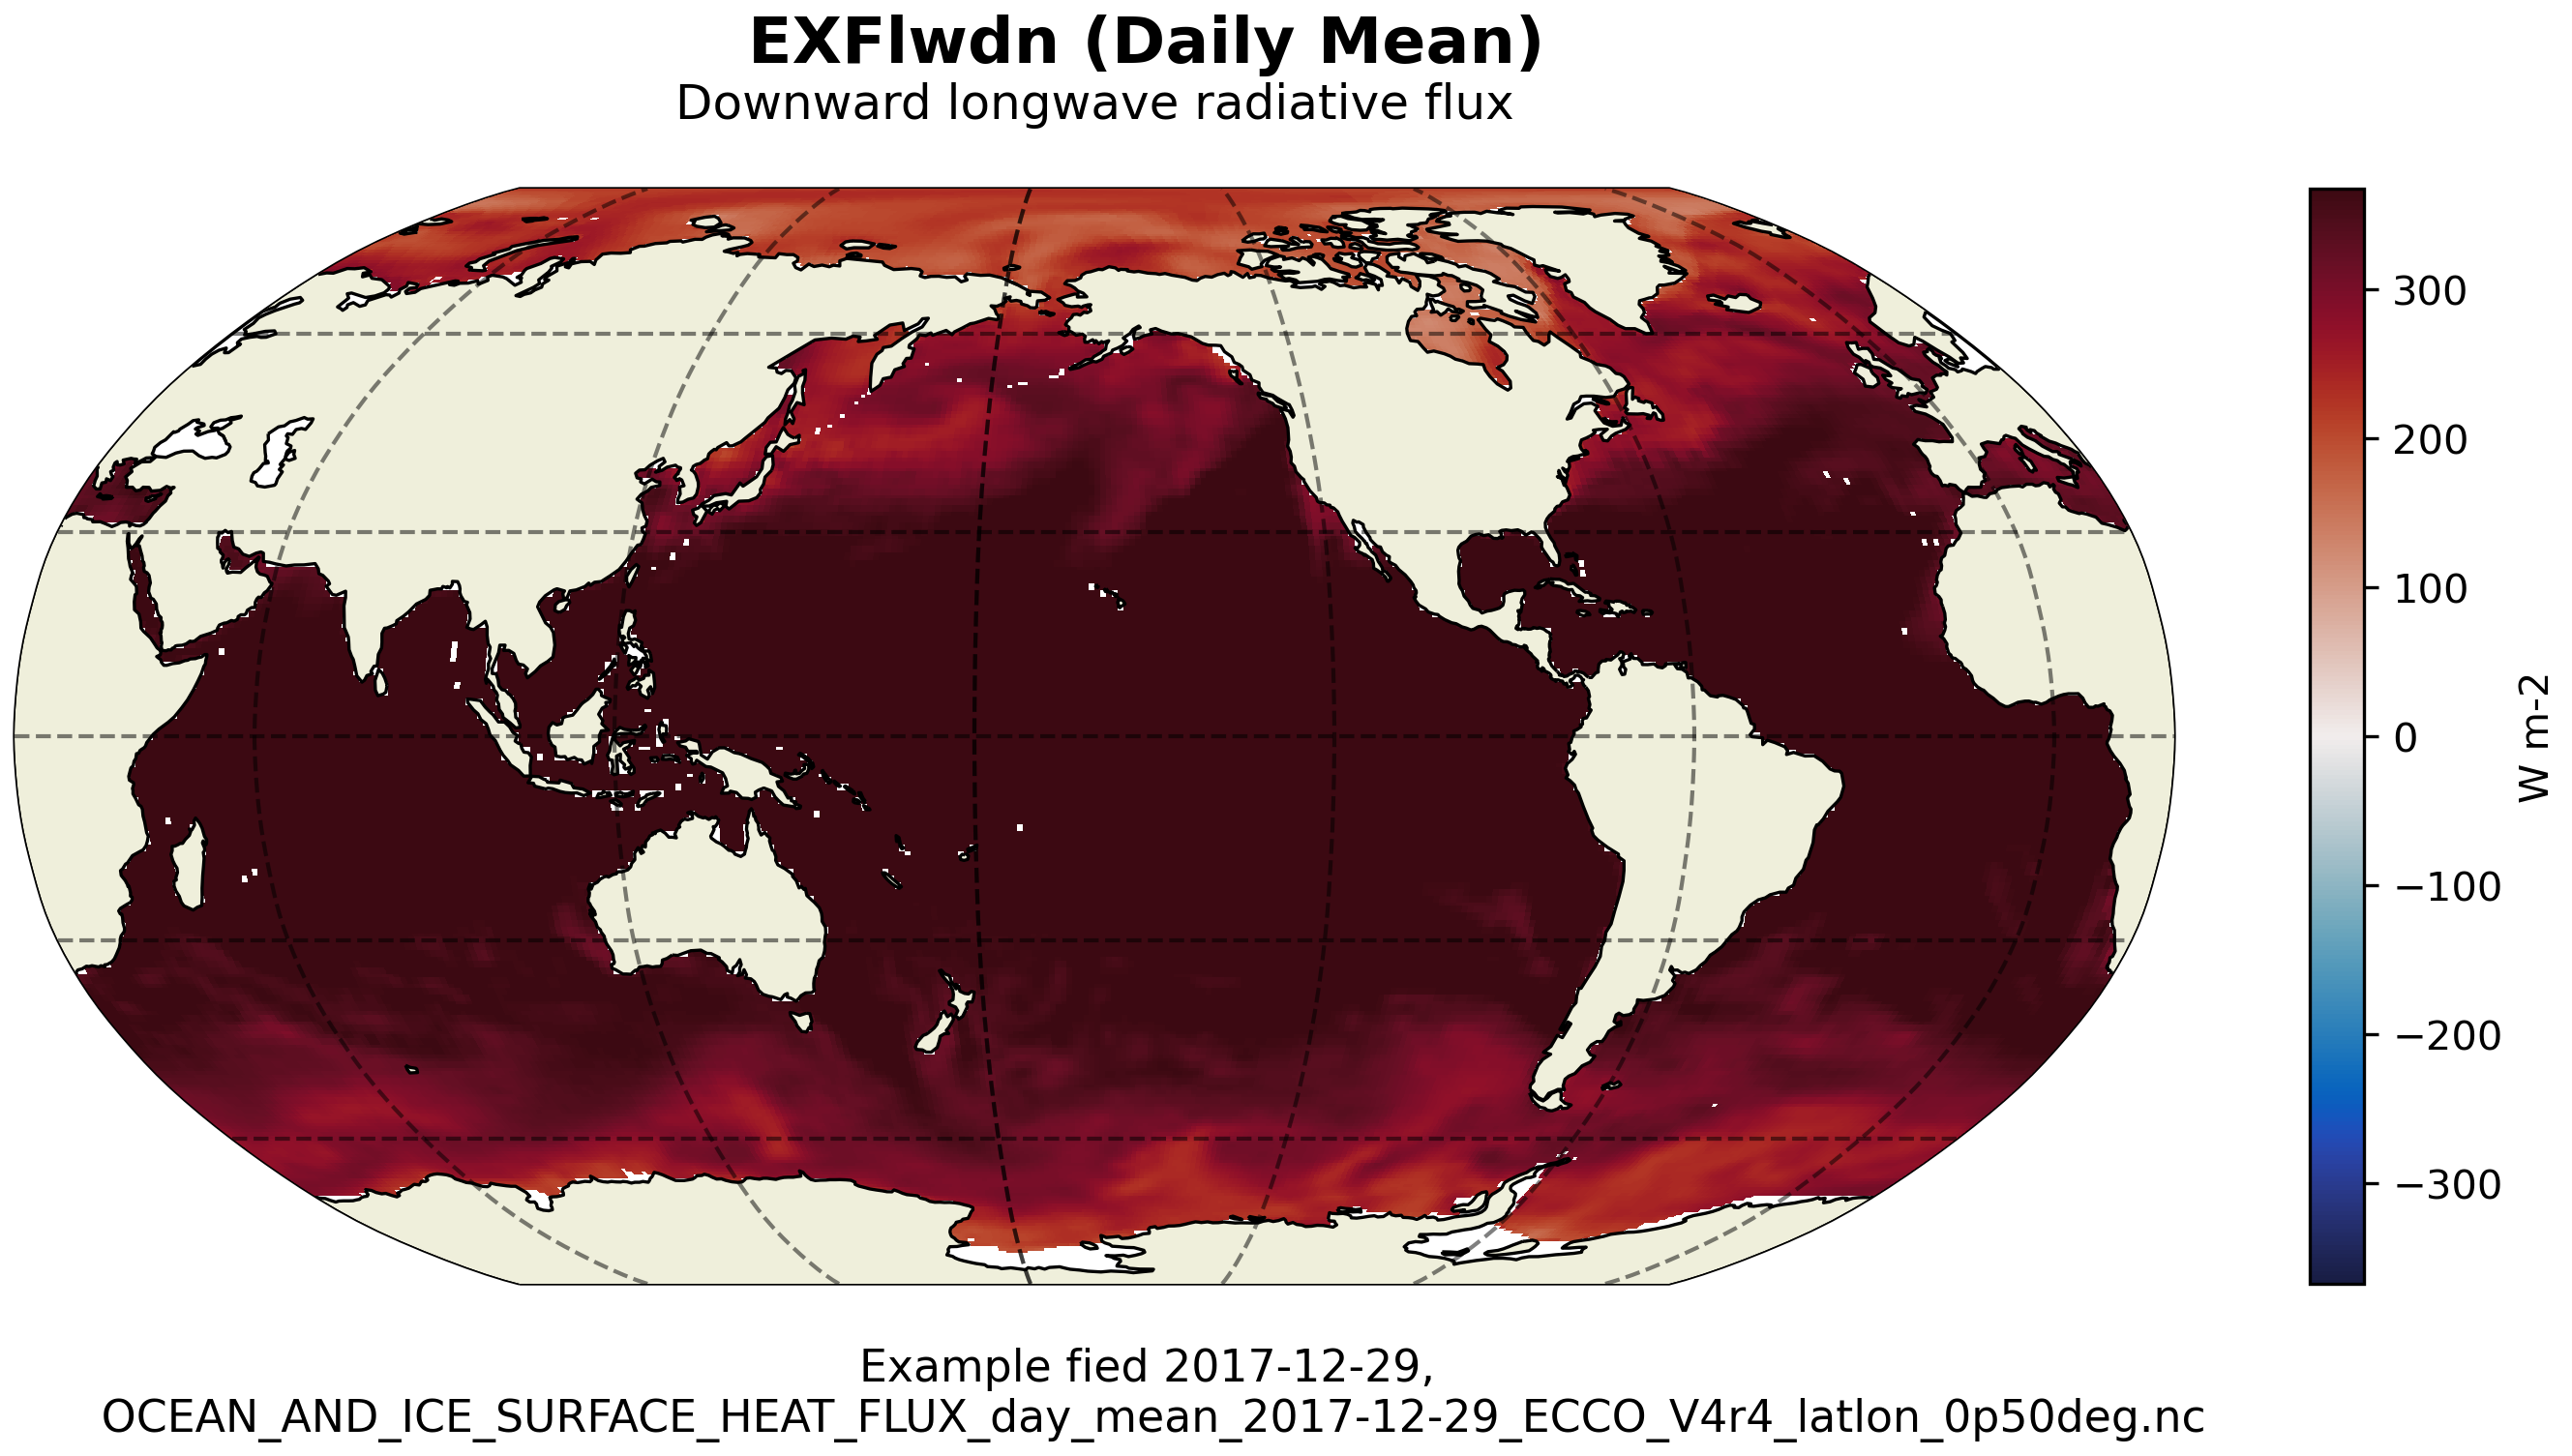
\includegraphics[width=\textwidth]{../images/plots/latlon_plots/Ocean_and_Sea-Ice_Surface_Heat_Fluxes/EXFlwdn.png}
\caption{Dataset: OCEAN\_AND\_ICE\_SURFACE\_HEAT\_FLUX Variable: EXFlwdn}
\label{tab:table-OCEAN_AND_ICE_SURFACE_HEAT_FLUX_EXFlwdn-Plot}
\end{figure}
\pagebreak
\subsubsection{Latlon Variable EXFlwnet}
\begin{longtable}{|p{0.06\textwidth}|p{0.41\textwidth}|p{0.39\textwidth}|p{0.06\textwidth}|}
\caption{CDL description of OCEAN\_AND\_ICE\_SURFACE\_HEAT\_FLUX's EXFlwnet variable}
\label{tab:table-OCEAN_AND_ICE_SURFACE_HEAT_FLUX_EXFlwnet} \\ 
\hline \endhead \hline \endfoot
\rowcolor{lightgray} \textbf{Storage Type} & \textbf{Variable Name} & \textbf{Description} & \textbf{Unit} \\ \hline
float32 & EXFlwnet & Net open ocean longwave radiative flux & W m-2 \\ \hline
\rowcolor{lightgray}  \multicolumn{4}{|p{1.00\textwidth}|}{\textbf{CDL Description}} \\ \hline
\multicolumn{4}{|p{1.00\textwidth}|}{\makecell{\parbox{1\textwidth}{float32 EXFlwnet(time, latitude, longitude)\\
\hspace*{0.5cm}EXFlwnet: \_FillValue = 9.96921e+36\\
\hspace*{0.5cm}EXFlwnet: coverage\_content\_type = modelResult\\
\hspace*{0.5cm}EXFlwnet: direction = >0 increases potential temperature (THETA)\\
\hspace*{0.5cm}EXFlwnet: long\_name = Net open ocean longwave radiative flux\\
\hspace*{0.5cm}EXFlwnet: standard\_name = surface\_net\_downward\_longwave\_flux\\
\hspace*{0.5cm}EXFlwnet: units = W m: 2\\
\hspace*{0.5cm}EXFlwnet: coordinates = time\\
\hspace*{0.5cm}EXFlwnet: valid\_min = : 144.3661346435547\\
\hspace*{0.5cm}EXFlwnet: valid\_max = 293.4114990234375}}} \\ \hline
\rowcolor{lightgray} \multicolumn{4}{|p{1.00\textwidth}|}{\textbf{Comments}} \\ \hline
\multicolumn{4}{|p{1\textwidth}|}{Net longwave radiative flux per unit area of open water (not covered by sea-ice). Note: net longwave radiation over open water calculated from downward longwave radiation (EXFlwdn) and upward longwave radiation from ocean and sea-ice thermal emission (Stefan-Boltzman law).} \\ \hline
\end{longtable}

\begin{figure}[H]
\centering
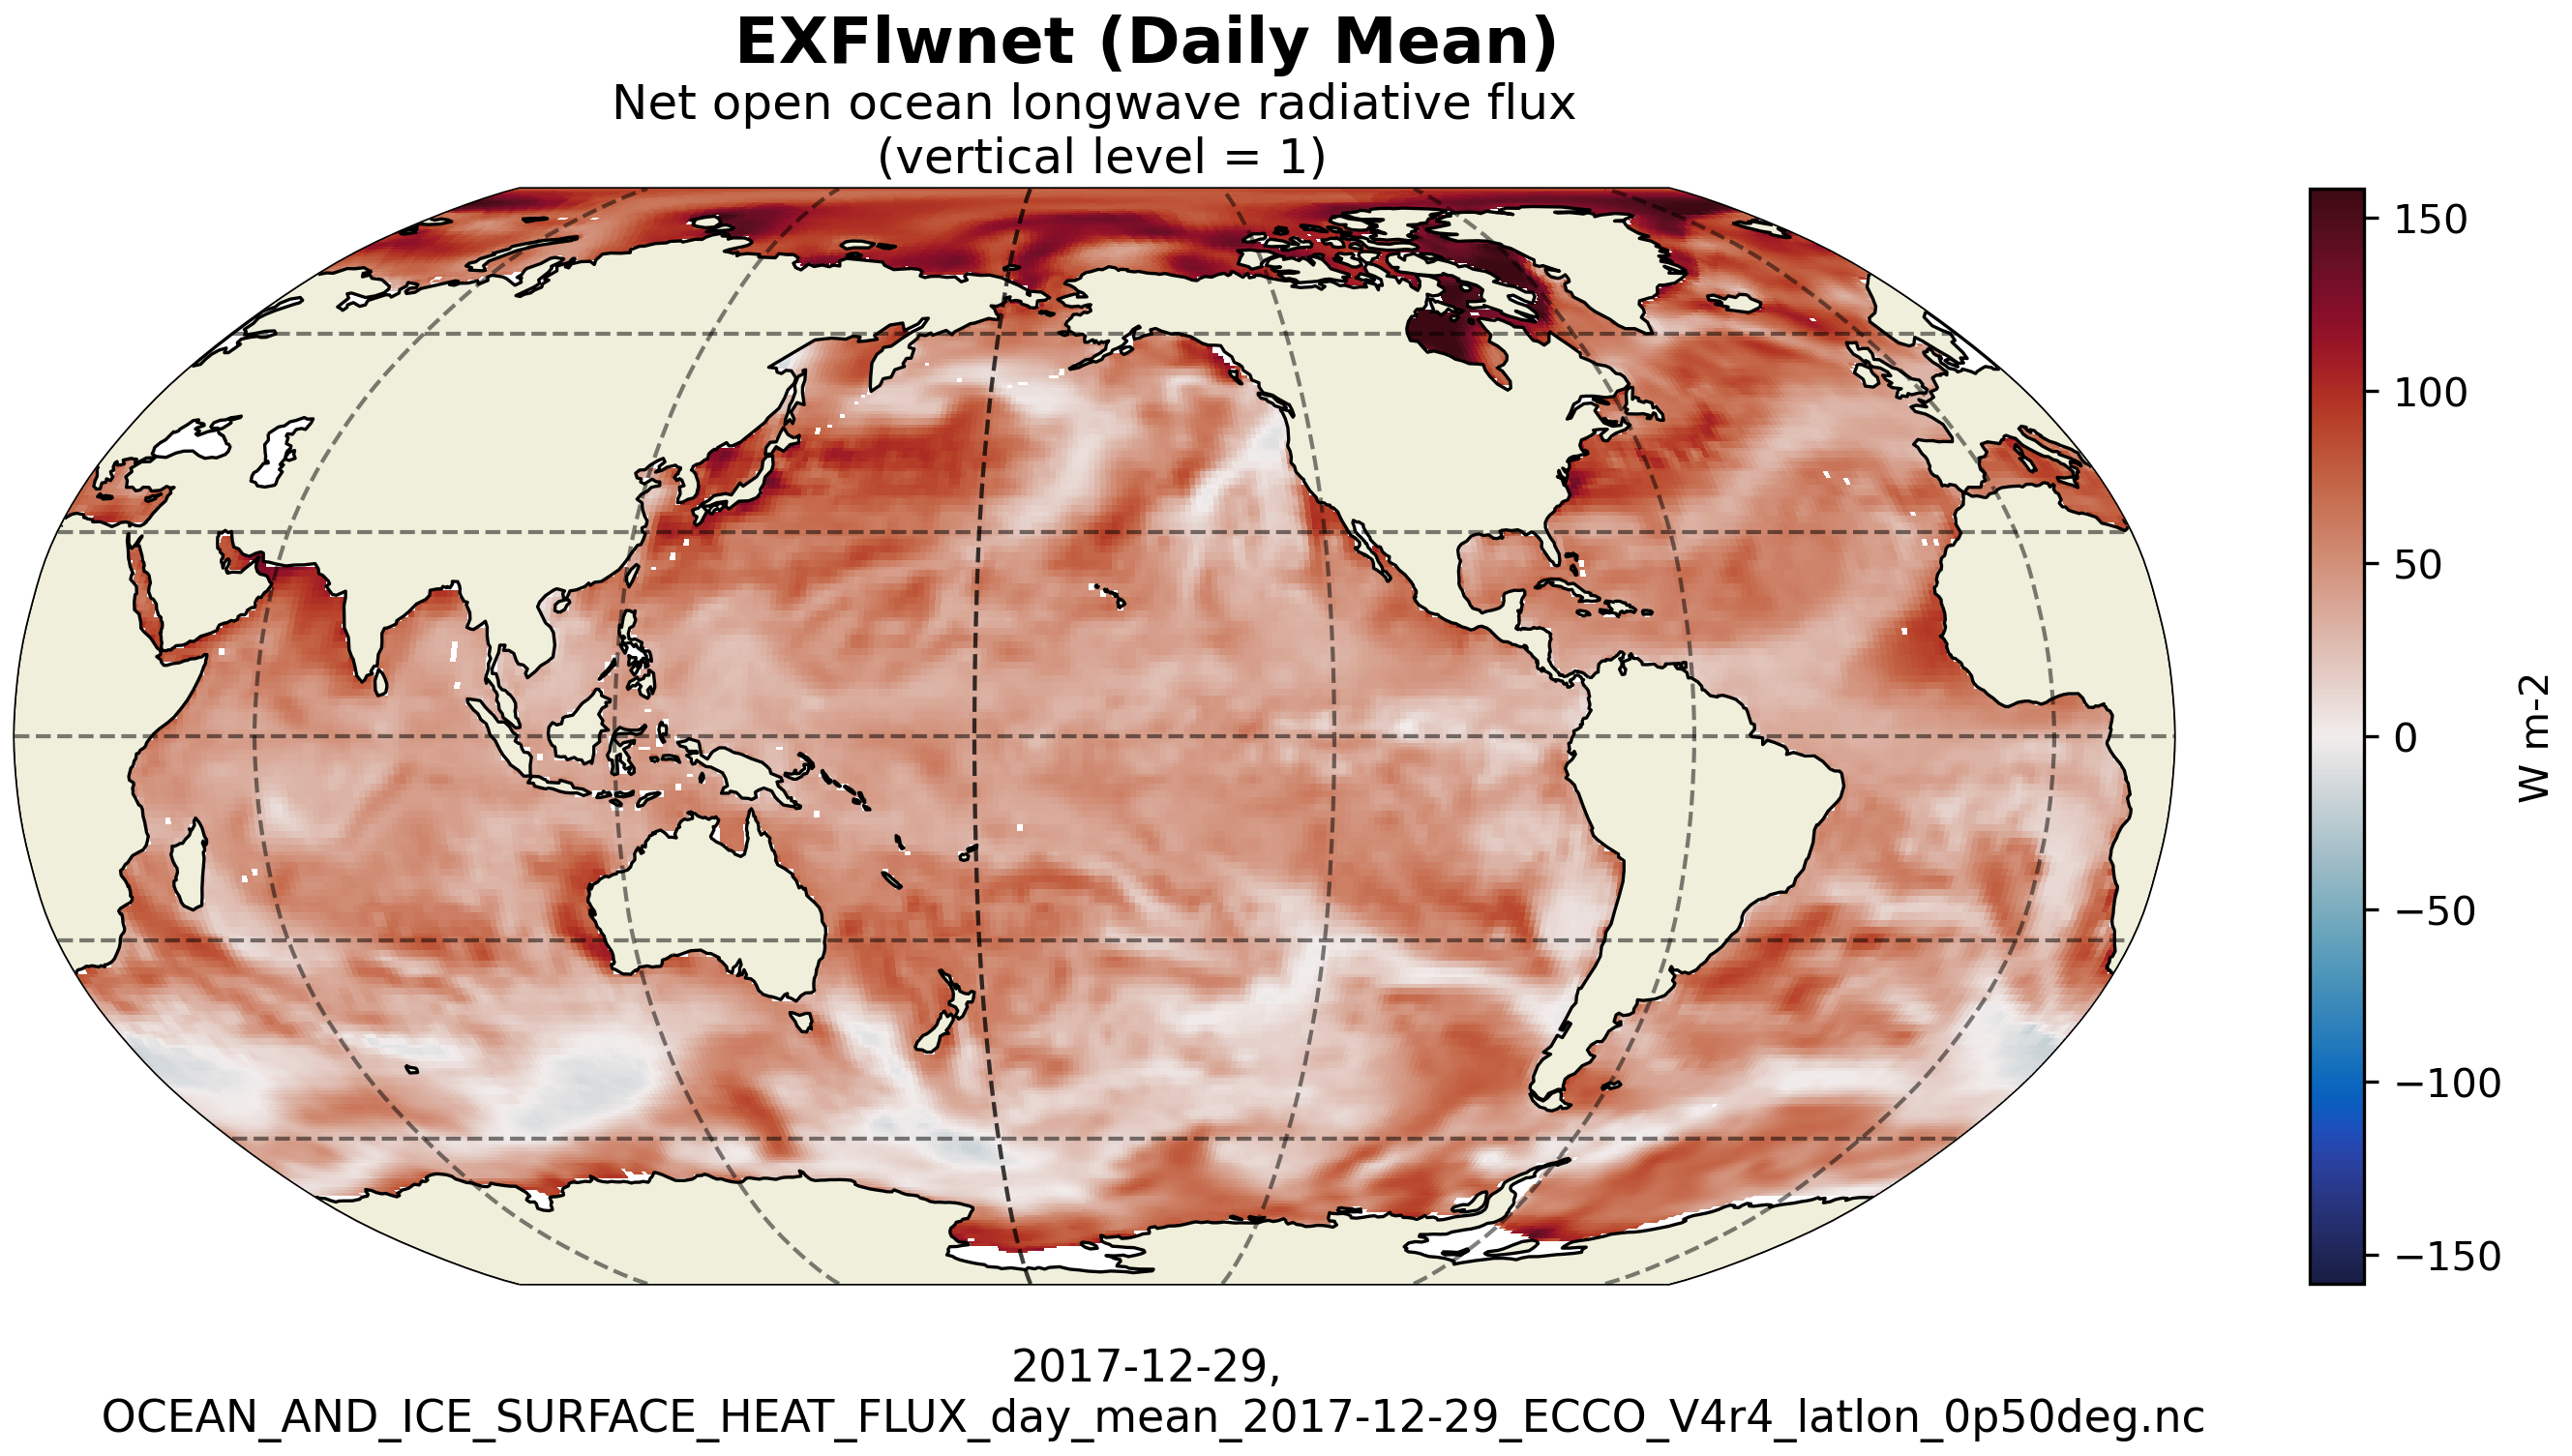
\includegraphics[width=\textwidth]{../images/plots/latlon_plots/Ocean_and_Sea-Ice_Surface_Heat_Fluxes/EXFlwnet.png}
\caption{Dataset: OCEAN\_AND\_ICE\_SURFACE\_HEAT\_FLUX Variable: EXFlwnet}
\label{tab:table-OCEAN_AND_ICE_SURFACE_HEAT_FLUX_EXFlwnet-Plot}
\end{figure}
\pagebreak
\subsubsection{Latlon Variable EXFqnet}
\begin{longtable}{|p{0.06\textwidth}|p{0.41\textwidth}|p{0.39\textwidth}|p{0.06\textwidth}|}
\caption{CDL description of OCEAN\_AND\_ICE\_SURFACE\_HEAT\_FLUX's EXFqnet variable}
\label{tab:table-OCEAN_AND_ICE_SURFACE_HEAT_FLUX_EXFqnet} \\ 
\hline \endhead \hline \endfoot
\rowcolor{lightgray} \textbf{Storage Type} & \textbf{Variable Name} & \textbf{Description} & \textbf{Unit} \\ \hline
float32 & EXFqnet & Open ocean net air-sea heat flux & W m-2 \\ \hline
\rowcolor{lightgray}  \multicolumn{4}{|p{1.00\textwidth}|}{\textbf{CDL Description}} \\ \hline
\multicolumn{4}{|p{1.00\textwidth}|}{\makecell{\parbox{1\textwidth}{float32 EXFqnet(time, latitude, longitude)\\
\hspace*{0.5cm}EXFqnet: \_FillValue = 9.96921e+36\\
\hspace*{0.5cm}EXFqnet: coverage\_content\_type = modelResult\\
\hspace*{0.5cm}EXFqnet: direction = >0 increases potential temperature (THETA)\\
\hspace*{0.5cm}EXFqnet: long\_name = Open ocean net air: sea heat flux\\
\hspace*{0.5cm}EXFqnet: units = W m: 2\\
\hspace*{0.5cm}EXFqnet: coordinates = time\\
\hspace*{0.5cm}EXFqnet: valid\_min = : 687.8736572265625\\
\hspace*{0.5cm}EXFqnet: valid\_max = 3408.977783203125}}} \\ \hline
\rowcolor{lightgray} \multicolumn{4}{|p{1.00\textwidth}|}{\textbf{Comments}} \\ \hline
\multicolumn{4}{|p{1\textwidth}|}{Net air-sea heat flux (turbulent and radiative) per unit area of open water (not covered by sea-ice). Note: net upward heat flux over open water, calculated as EXFlwnet+EXFswnet-EXFlh-EXFhs.} \\ \hline
\end{longtable}

\begin{figure}[H]
\centering
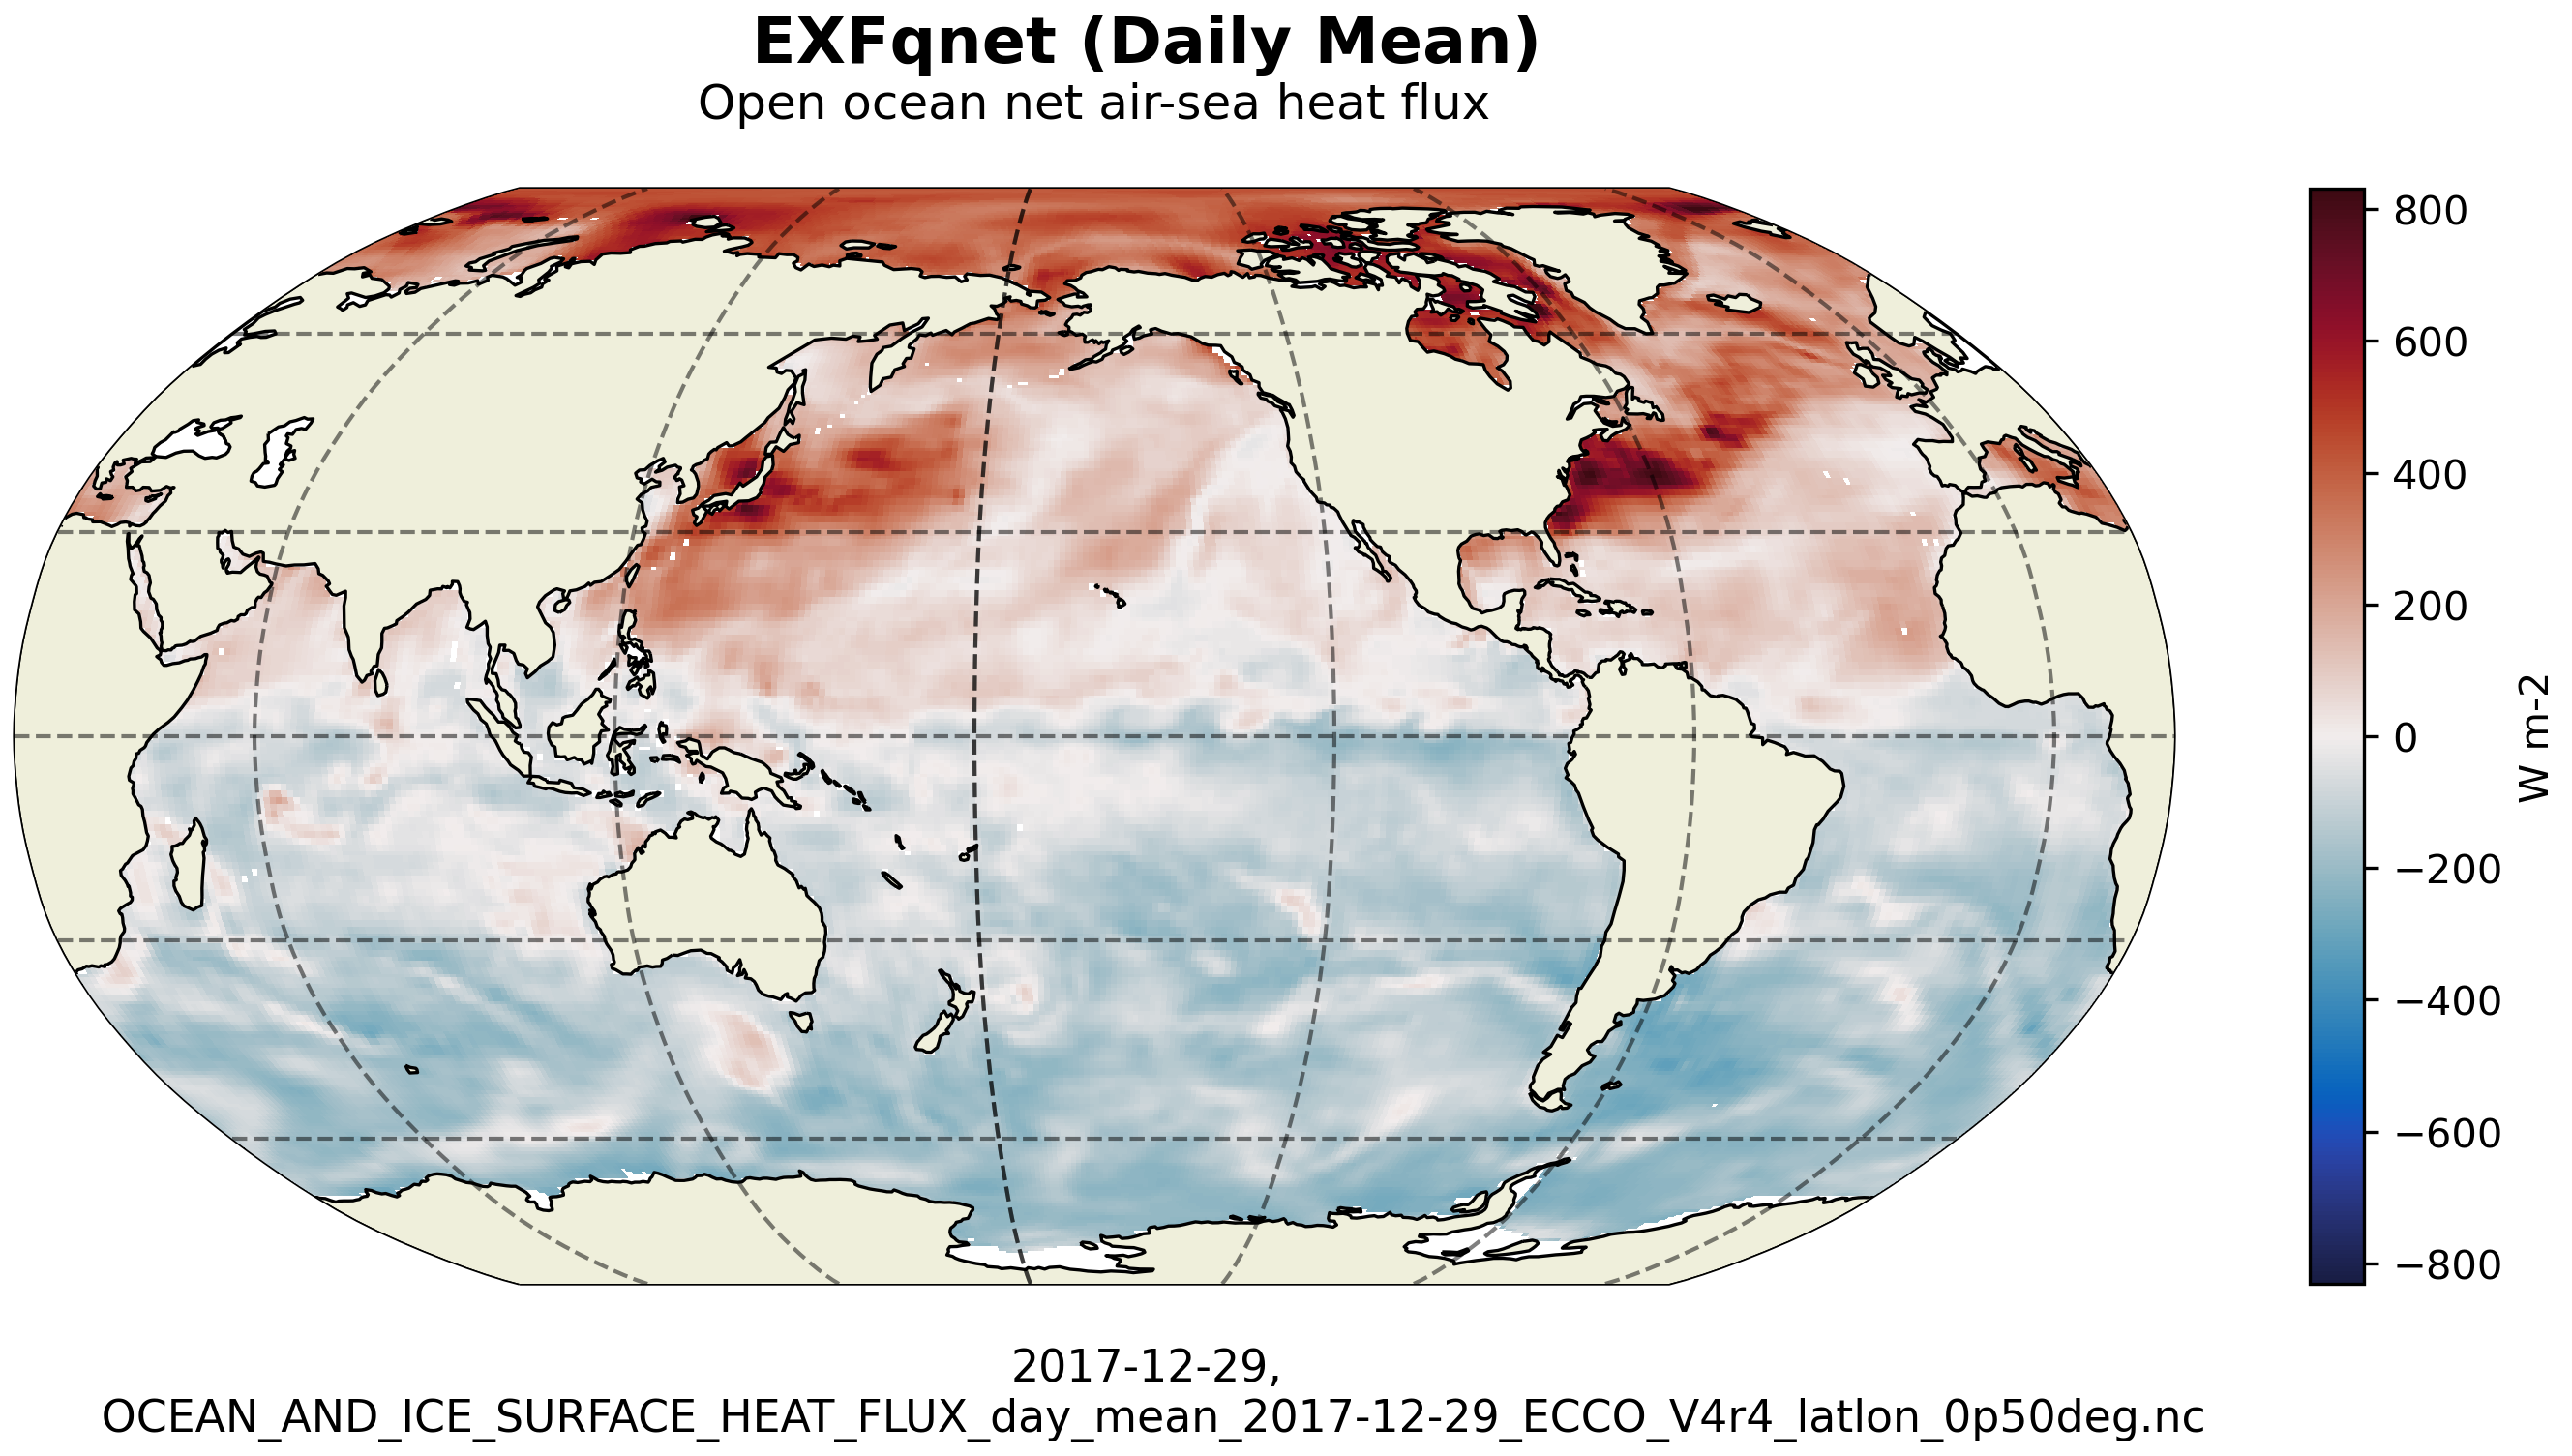
\includegraphics[width=\textwidth]{../images/plots/latlon_plots/Ocean_and_Sea-Ice_Surface_Heat_Fluxes/EXFqnet.png}
\caption{Dataset: OCEAN\_AND\_ICE\_SURFACE\_HEAT\_FLUX Variable: EXFqnet}
\label{tab:table-OCEAN_AND_ICE_SURFACE_HEAT_FLUX_EXFqnet-Plot}
\end{figure}
\pagebreak
\subsubsection{Latlon Variable EXFswdn}
\begin{longtable}{|p{0.06\textwidth}|p{0.41\textwidth}|p{0.39\textwidth}|p{0.06\textwidth}|}
\caption{CDL description of OCEAN\_AND\_ICE\_SURFACE\_HEAT\_FLUX's EXFswdn variable}
\label{tab:table-OCEAN_AND_ICE_SURFACE_HEAT_FLUX_EXFswdn} \\ 
\hline \endhead \hline \endfoot
\rowcolor{lightgray} \textbf{Storage Type} & \textbf{Variable Name} & \textbf{Description} & \textbf{Unit} \\ \hline
float32 & EXFswdn & Downwelling shortwave radiative flux & W m-2 \\ \hline
\rowcolor{lightgray}  \multicolumn{4}{|p{1.00\textwidth}|}{\textbf{CDL Description}} \\ \hline
\multicolumn{4}{|p{1.00\textwidth}|}{\makecell{\parbox{1\textwidth}{float32 EXFswdn(time, latitude, longitude)\\
\hspace*{0.5cm}EXFswdn: \_FillValue = 9.96921e+36\\
\hspace*{0.5cm}EXFswdn: coverage\_content\_type = modelResult\\
\hspace*{0.5cm}EXFswdn: direction = >0 increases potential temperature (THETA)\\
\hspace*{0.5cm}EXFswdn: long\_name = Downwelling shortwave radiative flux\\
\hspace*{0.5cm}EXFswdn: standard\_name = surface\_downwelling\_shortwave\_flux\_in\_air\\
\hspace*{0.5cm}EXFswdn: units = W m: 2\\
\hspace*{0.5cm}EXFswdn: coordinates = time\\
\hspace*{0.5cm}EXFswdn: valid\_min = : 224.63368225097656\\
\hspace*{0.5cm}EXFswdn: valid\_max = 707.345947265625}}} \\ \hline
\rowcolor{lightgray} \multicolumn{4}{|p{1.00\textwidth}|}{\textbf{Comments}} \\ \hline
\multicolumn{4}{|p{1\textwidth}|}{Downward shortwave radiative flux. Note: sum of ERA-Interim downward shortwave radiation and the control adjustment from ocean state estimation.} \\ \hline
\end{longtable}

\begin{figure}[H]
\centering
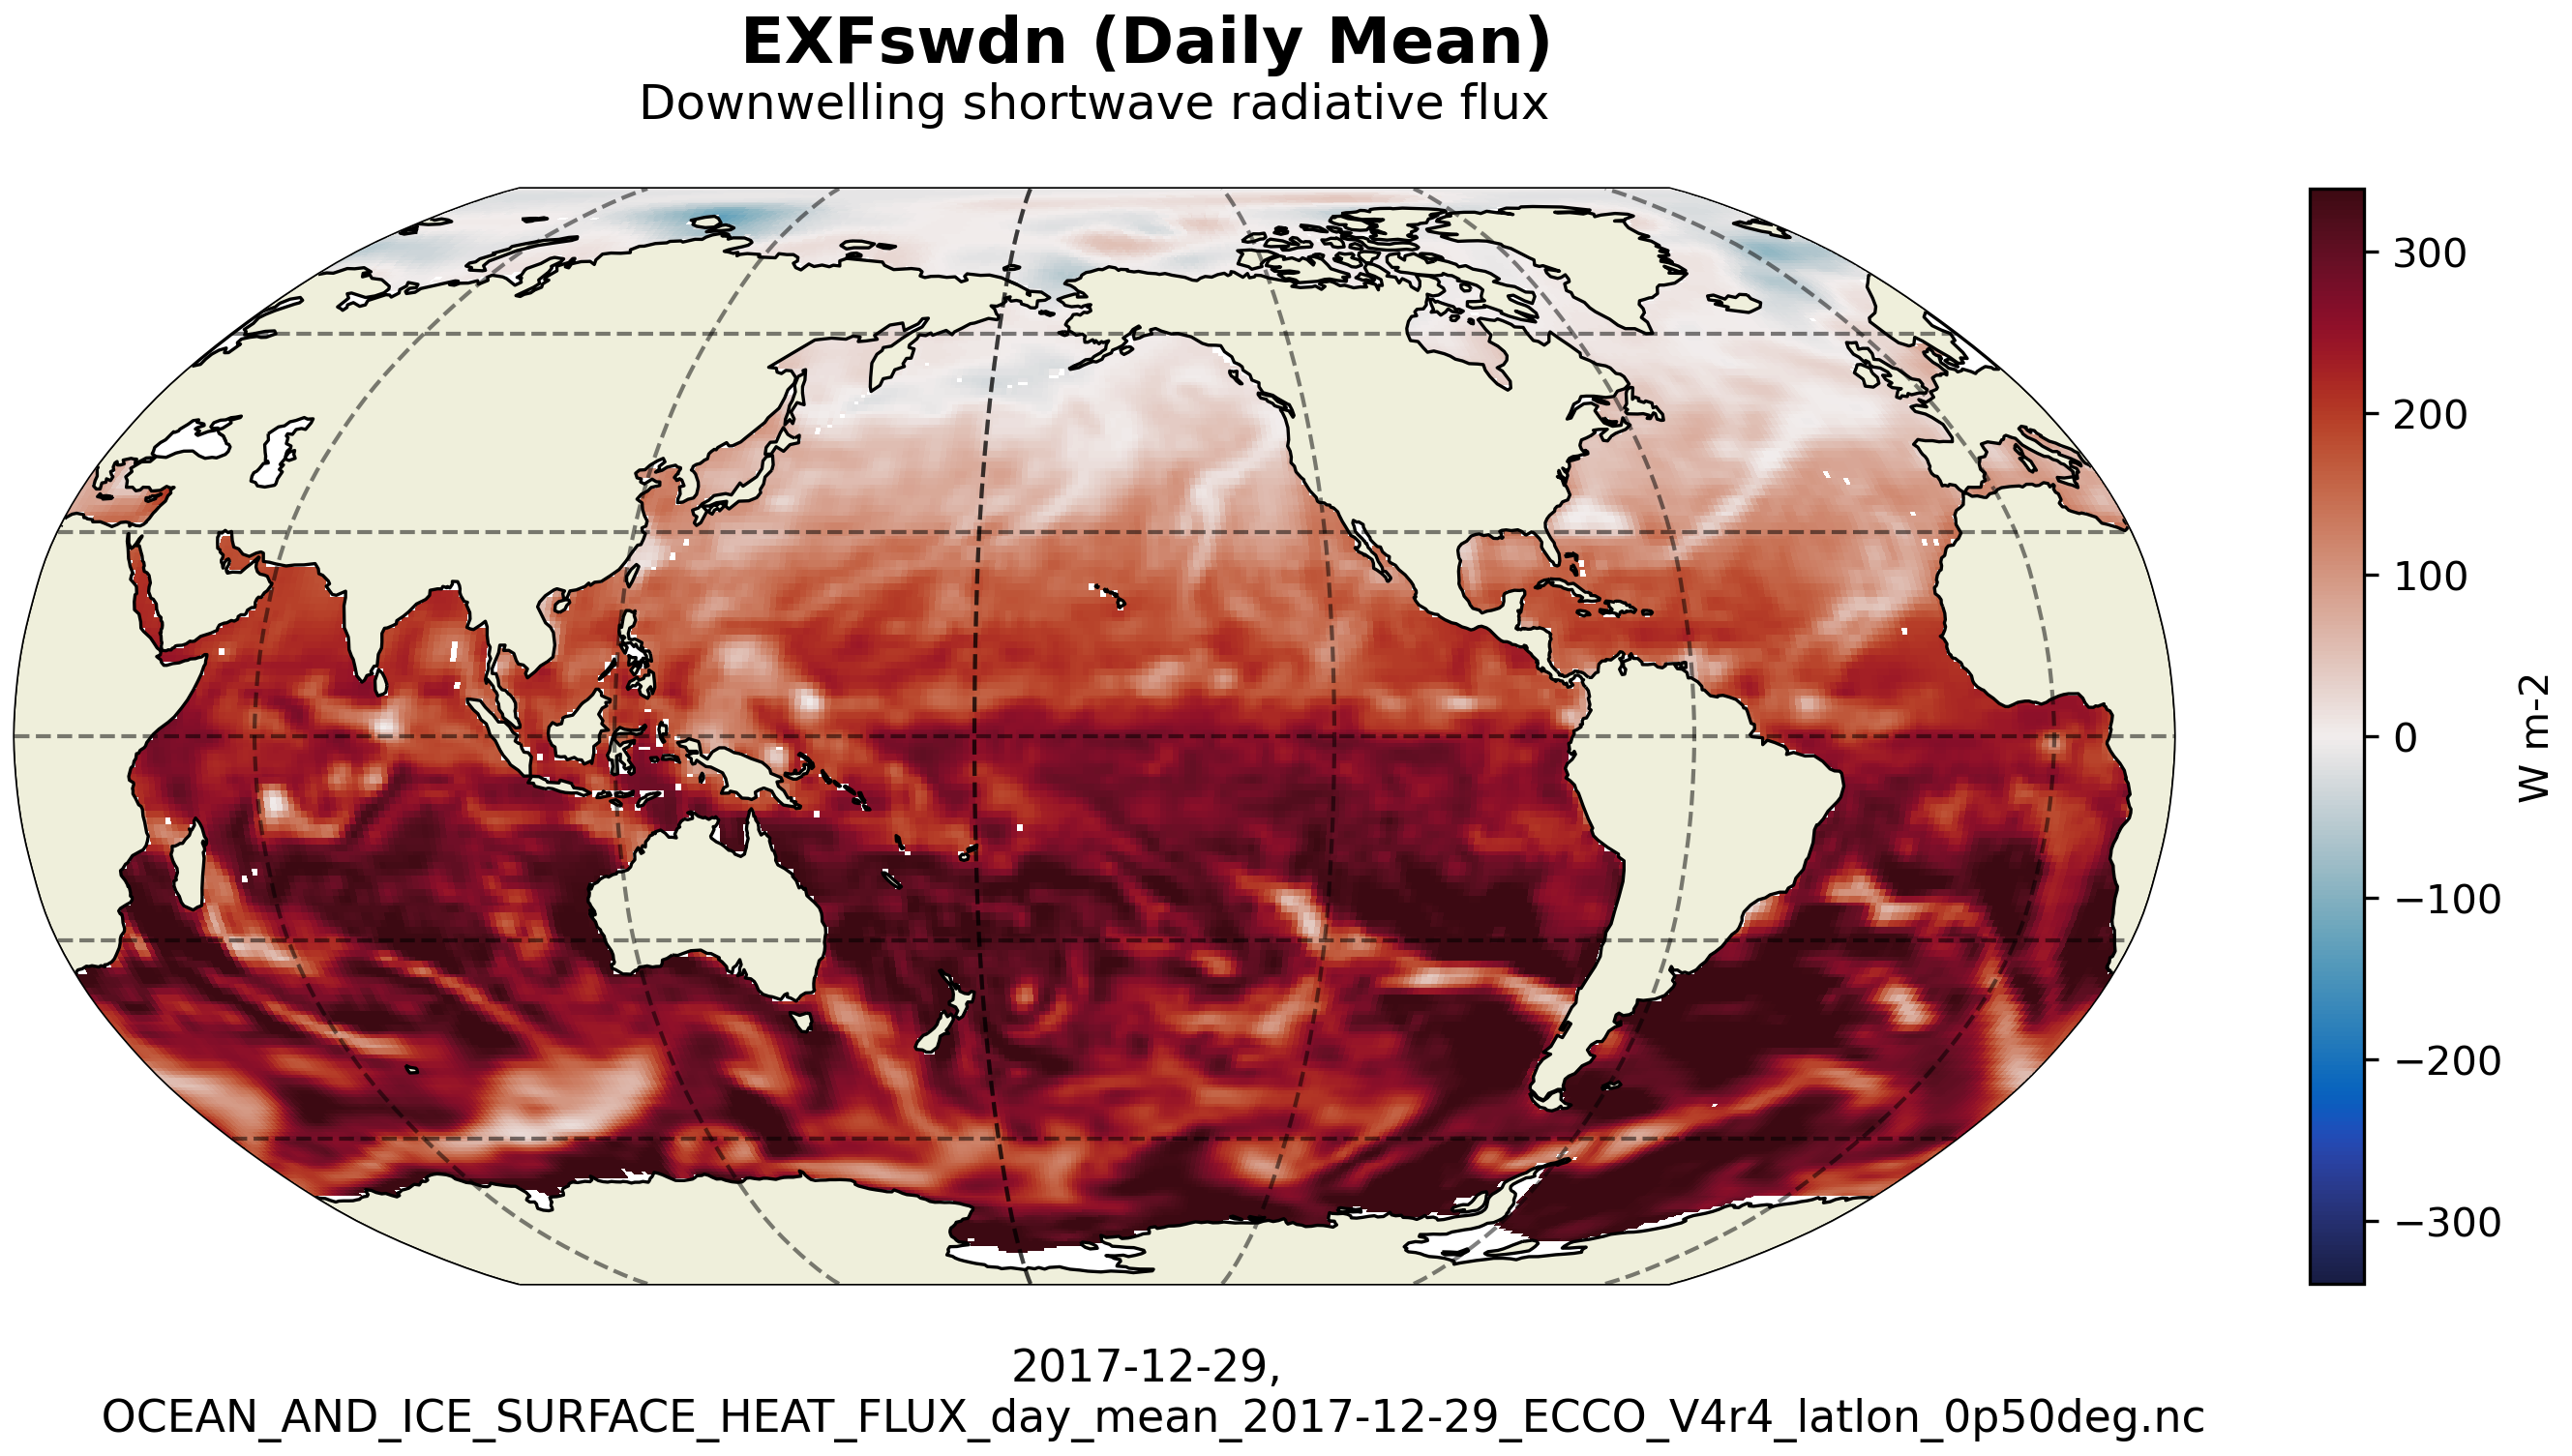
\includegraphics[width=\textwidth]{../images/plots/latlon_plots/Ocean_and_Sea-Ice_Surface_Heat_Fluxes/EXFswdn.png}
\caption{Dataset: OCEAN\_AND\_ICE\_SURFACE\_HEAT\_FLUX Variable: EXFswdn}
\label{tab:table-OCEAN_AND_ICE_SURFACE_HEAT_FLUX_EXFswdn-Plot}
\end{figure}
\pagebreak
\subsubsection{Latlon Variable EXFswnet}
\begin{longtable}{|p{0.06\textwidth}|p{0.41\textwidth}|p{0.39\textwidth}|p{0.06\textwidth}|}
\caption{CDL description of OCEAN\_AND\_ICE\_SURFACE\_HEAT\_FLUX's EXFswnet variable}
\label{tab:table-OCEAN_AND_ICE_SURFACE_HEAT_FLUX_EXFswnet} \\ 
\hline \endhead \hline \endfoot
\rowcolor{lightgray} \textbf{Storage Type} & \textbf{Variable Name} & \textbf{Description} & \textbf{Unit} \\ \hline
float32 & EXFswnet & Open ocean net shortwave radiative flux & W m-2 \\ \hline
\rowcolor{lightgray}  \multicolumn{4}{|p{1.00\textwidth}|}{\textbf{CDL Description}} \\ \hline
\multicolumn{4}{|p{1.00\textwidth}|}{\makecell{\parbox{1\textwidth}{float32 EXFswnet(time, latitude, longitude)\\
\hspace*{0.5cm}EXFswnet: \_FillValue = 9.96921e+36\\
\hspace*{0.5cm}EXFswnet: coverage\_content\_type = modelResult\\
\hspace*{0.5cm}EXFswnet: direction = >0 increases potential temperature (THETA)\\
\hspace*{0.5cm}EXFswnet: long\_name = Open ocean net shortwave radiative flux\\
\hspace*{0.5cm}EXFswnet: standard\_name = surface\_net\_downward\_shortwave\_flux\\
\hspace*{0.5cm}EXFswnet: units = W m: 2\\
\hspace*{0.5cm}EXFswnet: coordinates = time\\
\hspace*{0.5cm}EXFswnet: valid\_min = : 655.6171264648438\\
\hspace*{0.5cm}EXFswnet: valid\_max = 193.89297485351562}}} \\ \hline
\rowcolor{lightgray} \multicolumn{4}{|p{1.00\textwidth}|}{\textbf{Comments}} \\ \hline
\multicolumn{4}{|p{1\textwidth}|}{Net shortwave radiative flux per unit area of open water (not covered by sea-ice). Note: net shortwave radiation over open water calculated from downward shortwave flux (EXFswdn) and ocean surface albdeo.} \\ \hline
\end{longtable}

\begin{figure}[H]
\centering
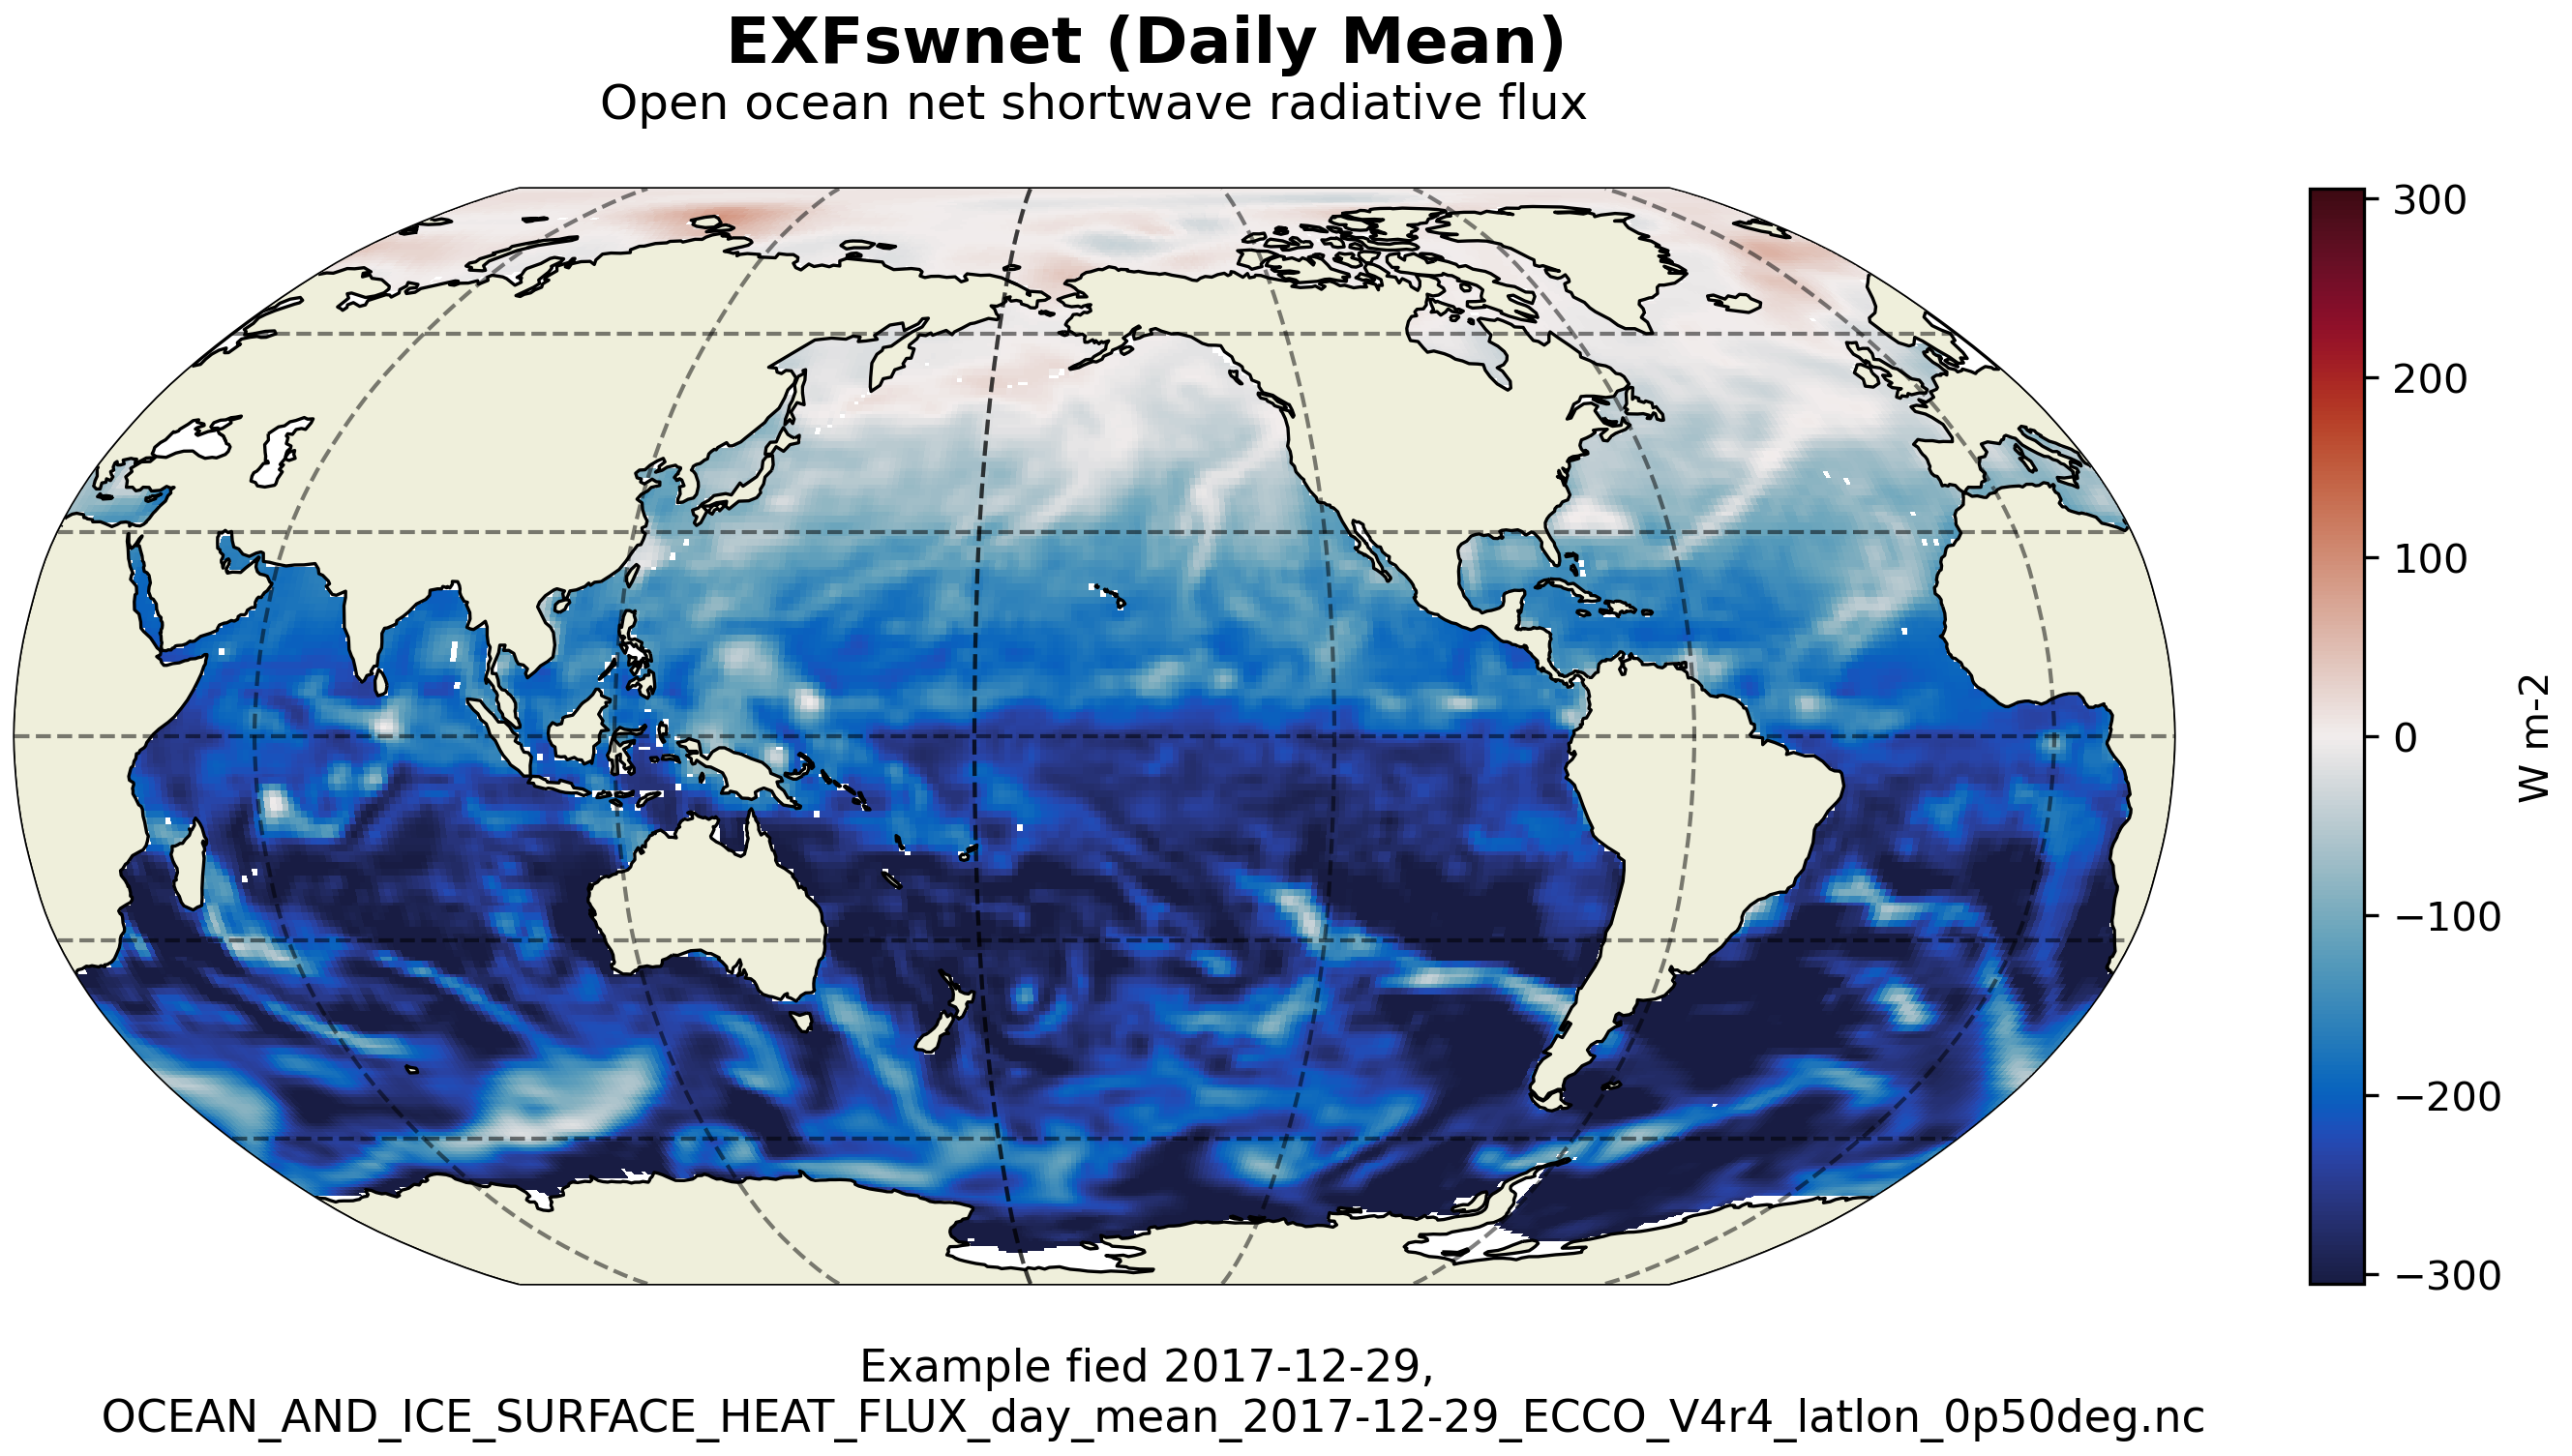
\includegraphics[width=\textwidth]{../images/plots/latlon_plots/Ocean_and_Sea-Ice_Surface_Heat_Fluxes/EXFswnet.png}
\caption{Dataset: OCEAN\_AND\_ICE\_SURFACE\_HEAT\_FLUX Variable: EXFswnet}
\label{tab:table-OCEAN_AND_ICE_SURFACE_HEAT_FLUX_EXFswnet-Plot}
\end{figure}
\pagebreak
\subsubsection{Latlon Variable SIaaflux}
\begin{longtable}{|p{0.06\textwidth}|p{0.41\textwidth}|p{0.39\textwidth}|p{0.06\textwidth}|}
\caption{CDL description of OCEAN\_AND\_ICE\_SURFACE\_HEAT\_FLUX's SIaaflux variable}
\label{tab:table-OCEAN_AND_ICE_SURFACE_HEAT_FLUX_SIaaflux} \\ 
\hline \endhead \hline \endfoot
\rowcolor{lightgray} \textbf{Storage Type} & \textbf{Variable Name} & \textbf{Description} & \textbf{Unit} \\ \hline
float32 & SIaaflux & Conservative ocean and sea-ice advective heat flux adjustment & W m-2 \\ \hline
\rowcolor{lightgray}  \multicolumn{4}{|p{1.00\textwidth}|}{\textbf{CDL Description}} \\ \hline
\multicolumn{4}{|p{1.00\textwidth}|}{\makecell{\parbox{1\textwidth}{float32 SIaaflux(time, latitude, longitude)\\
\hspace*{0.5cm}SIaaflux: \_FillValue = 9.96921e+36\\
\hspace*{0.5cm}SIaaflux: coverage\_content\_type = modelResult\\
\hspace*{0.5cm}SIaaflux: direction = >0 decrease potential temperature (THETA)\\
\hspace*{0.5cm}SIaaflux: long\_name = Conservative ocean and sea: ice advective heat flux adjustment\\
\hspace*{0.5cm}SIaaflux: units = W m: 2\\
\hspace*{0.5cm}SIaaflux: coordinates = time\\
\hspace*{0.5cm}SIaaflux: valid\_min = : 16.214622497558594\\
\hspace*{0.5cm}SIaaflux: valid\_max = 50.35451889038086}}} \\ \hline
\rowcolor{lightgray} \multicolumn{4}{|p{1.00\textwidth}|}{\textbf{Comments}} \\ \hline
\multicolumn{4}{|p{1\textwidth}|}{Heat flux associated with the temperature difference between sea surface temperature and sea-ice (assume 0 degree C in the model). Note: heat flux needed to melt/freeze sea-ice at 0 degC to sea water at the ocean surface (at sea surface temperature), excluding the latent heat of fusion.} \\ \hline
\end{longtable}

\begin{figure}[H]
\centering
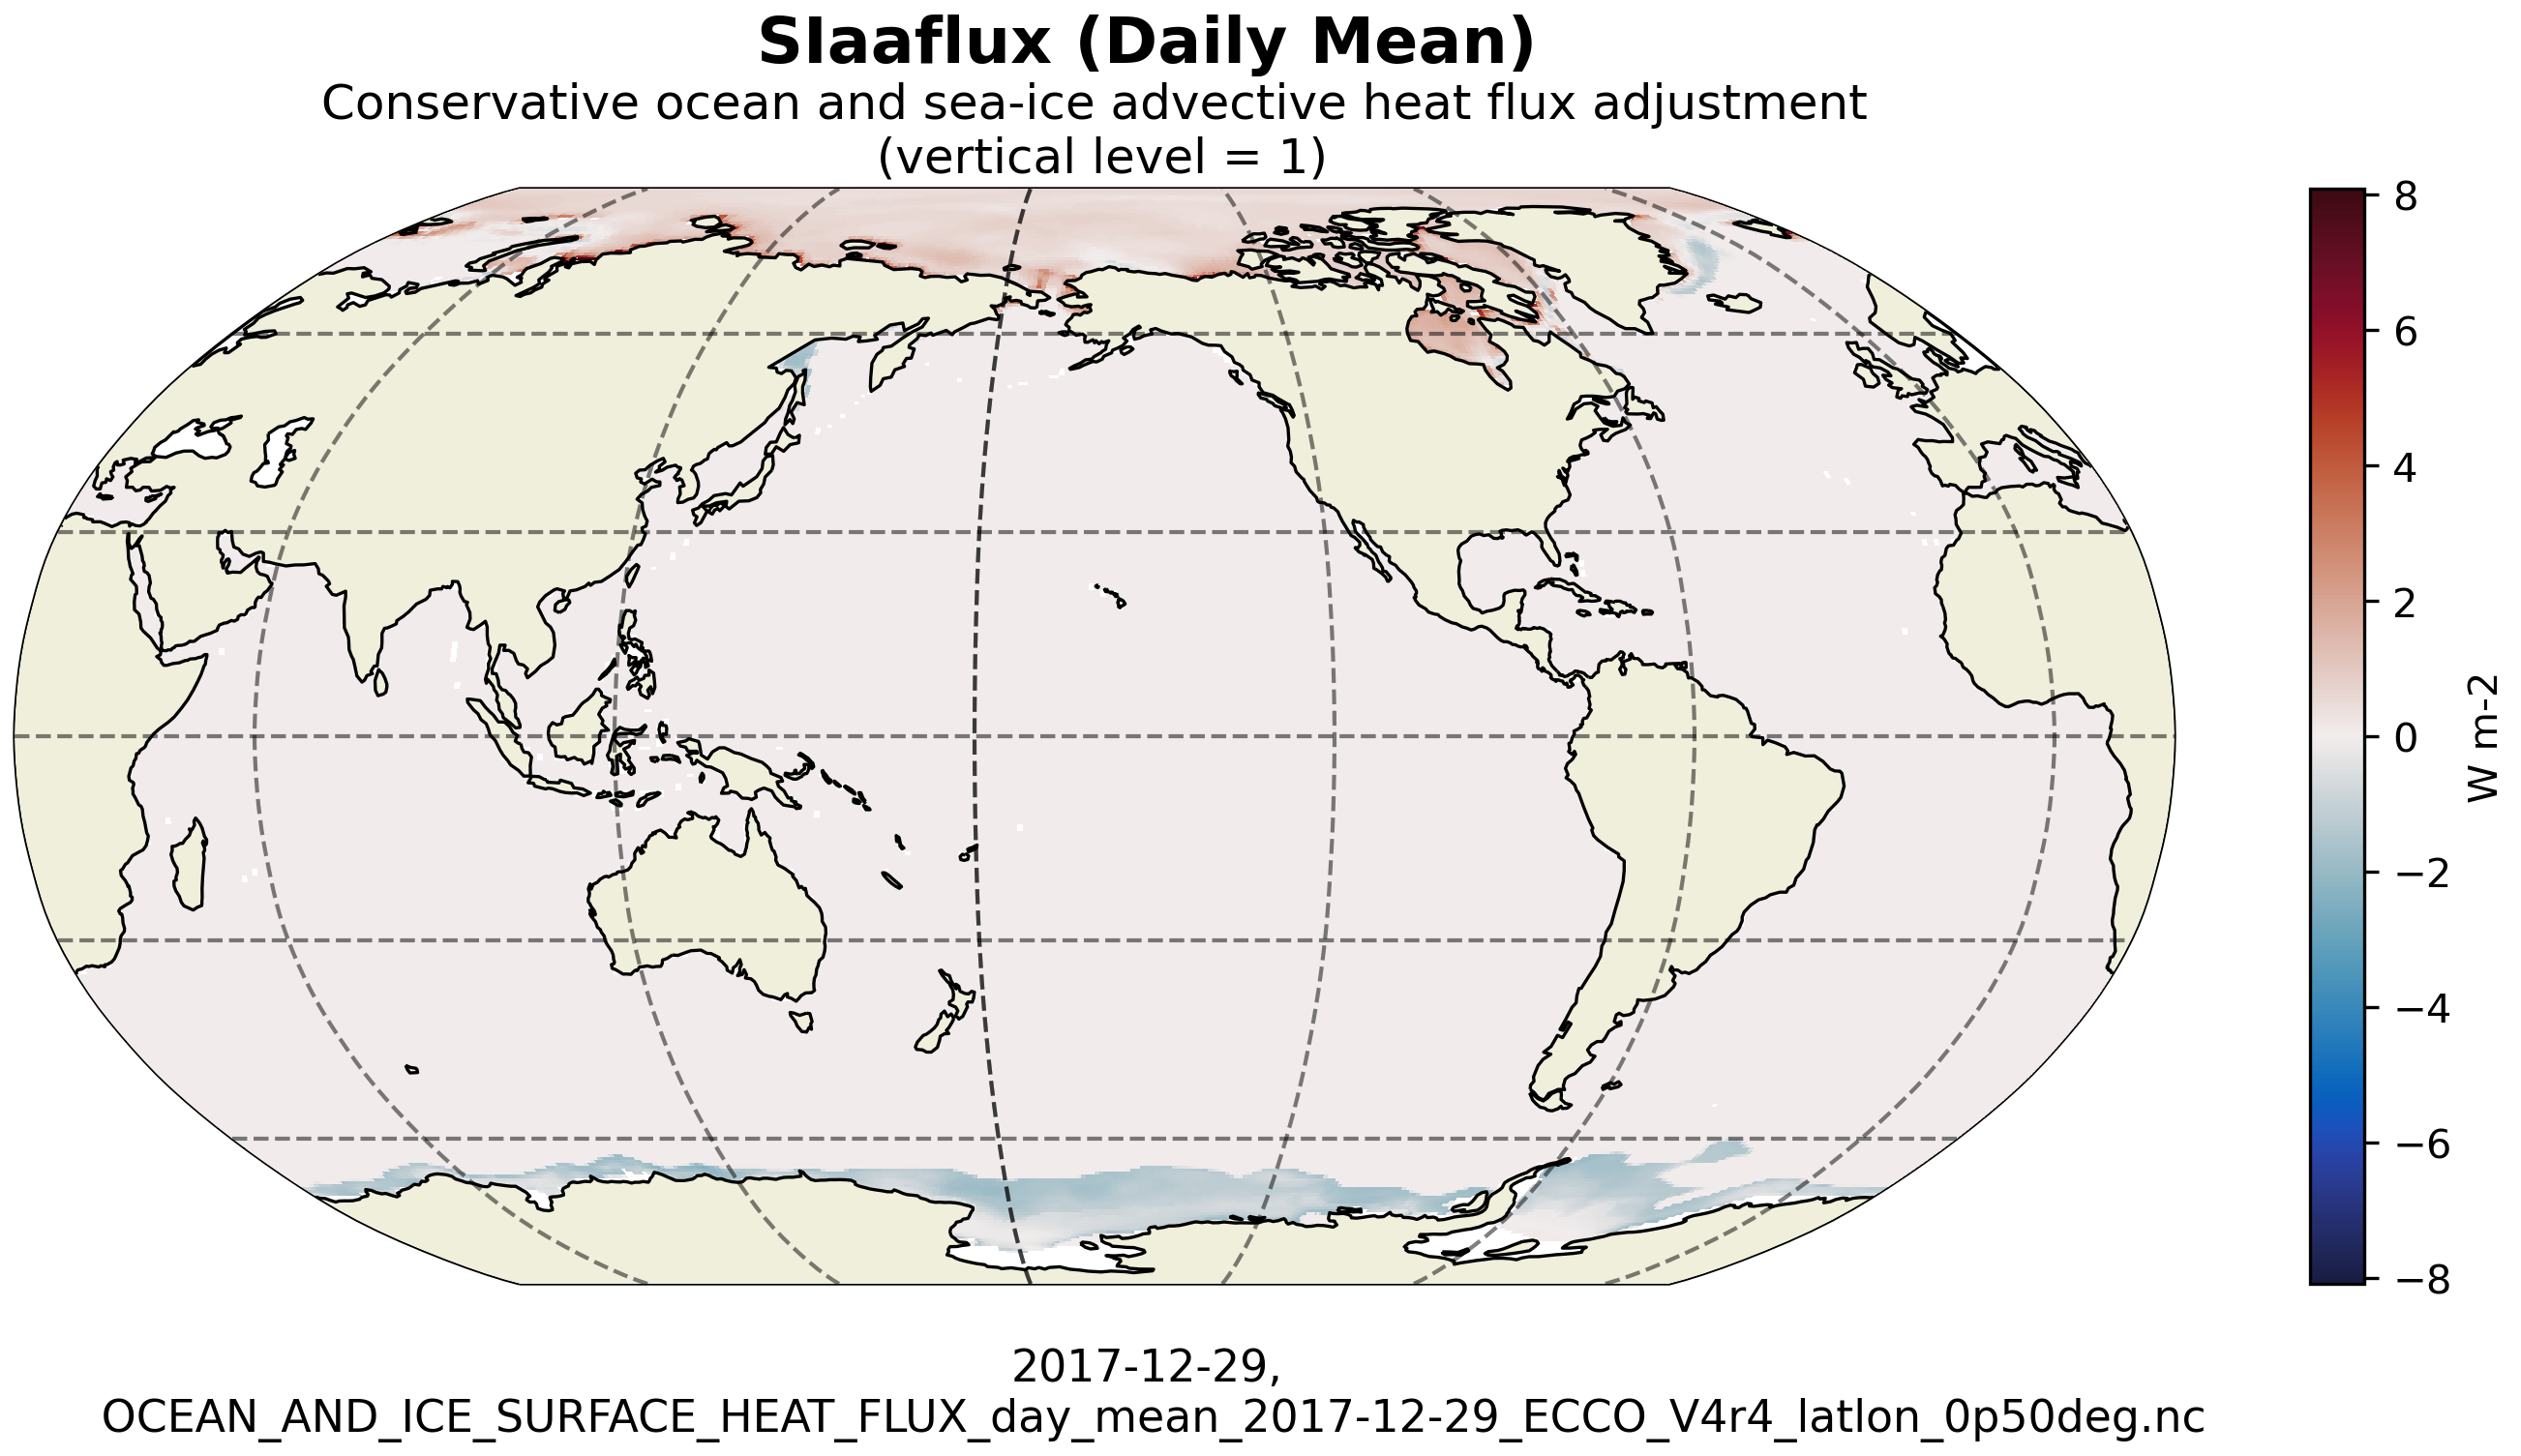
\includegraphics[width=\textwidth]{../images/plots/latlon_plots/Ocean_and_Sea-Ice_Surface_Heat_Fluxes/SIaaflux.png}
\caption{Dataset: OCEAN\_AND\_ICE\_SURFACE\_HEAT\_FLUX Variable: SIaaflux}
\label{tab:table-OCEAN_AND_ICE_SURFACE_HEAT_FLUX_SIaaflux-Plot}
\end{figure}
\pagebreak
\subsubsection{Latlon Variable SIatmQnt}
\begin{longtable}{|p{0.06\textwidth}|p{0.41\textwidth}|p{0.39\textwidth}|p{0.06\textwidth}|}
\caption{CDL description of OCEAN\_AND\_ICE\_SURFACE\_HEAT\_FLUX's SIatmQnt variable}
\label{tab:table-OCEAN_AND_ICE_SURFACE_HEAT_FLUX_SIatmQnt} \\ 
\hline \endhead \hline \endfoot
\rowcolor{lightgray} \textbf{Storage Type} & \textbf{Variable Name} & \textbf{Description} & \textbf{Unit} \\ \hline
float32 & SIatmQnt & Net upward heat flux to the atmosphere & W m-2 \\ \hline
\rowcolor{lightgray}  \multicolumn{4}{|p{1.00\textwidth}|}{\textbf{CDL Description}} \\ \hline
\multicolumn{4}{|p{1.00\textwidth}|}{\makecell{\parbox{1\textwidth}{float32 SIatmQnt(time, latitude, longitude)\\
\hspace*{0.5cm}SIatmQnt: \_FillValue = 9.96921e+36\\
\hspace*{0.5cm}SIatmQnt: coverage\_content\_type = modelResult\\
\hspace*{0.5cm}SIatmQnt: direction = >0 upward\\
decreases ocean temperature\\
\hspace*{0.5cm}SIatmQnt: long\_name = Net upward heat flux to the atmosphere\\
\hspace*{0.5cm}SIatmQnt: standard\_name = surface\_upward\_heat\_flux\_in\_air\\
\hspace*{0.5cm}SIatmQnt: units = W m: 2\\
\hspace*{0.5cm}SIatmQnt: coordinates = time\\
\hspace*{0.5cm}SIatmQnt: valid\_min = : 756.0607299804688\\
\hspace*{0.5cm}SIatmQnt: valid\_max = 1704.7703857421875}}} \\ \hline
\rowcolor{lightgray} \multicolumn{4}{|p{1.00\textwidth}|}{\textbf{Comments}} \\ \hline
\multicolumn{4}{|p{1\textwidth}|}{Net upward heat flux to the atmosphere across open water and sea-ice or snow surfaces. Note: nonzero SIatmQnt may not be associated with a change in ocean potential temperature due to sea-ice growth or melting. To calculate total ocean heat content changes use the variable TFLUX which also accounts for changing ocean mass (e.g. oceFWflx).} \\ \hline
\end{longtable}

\begin{figure}[H]
\centering
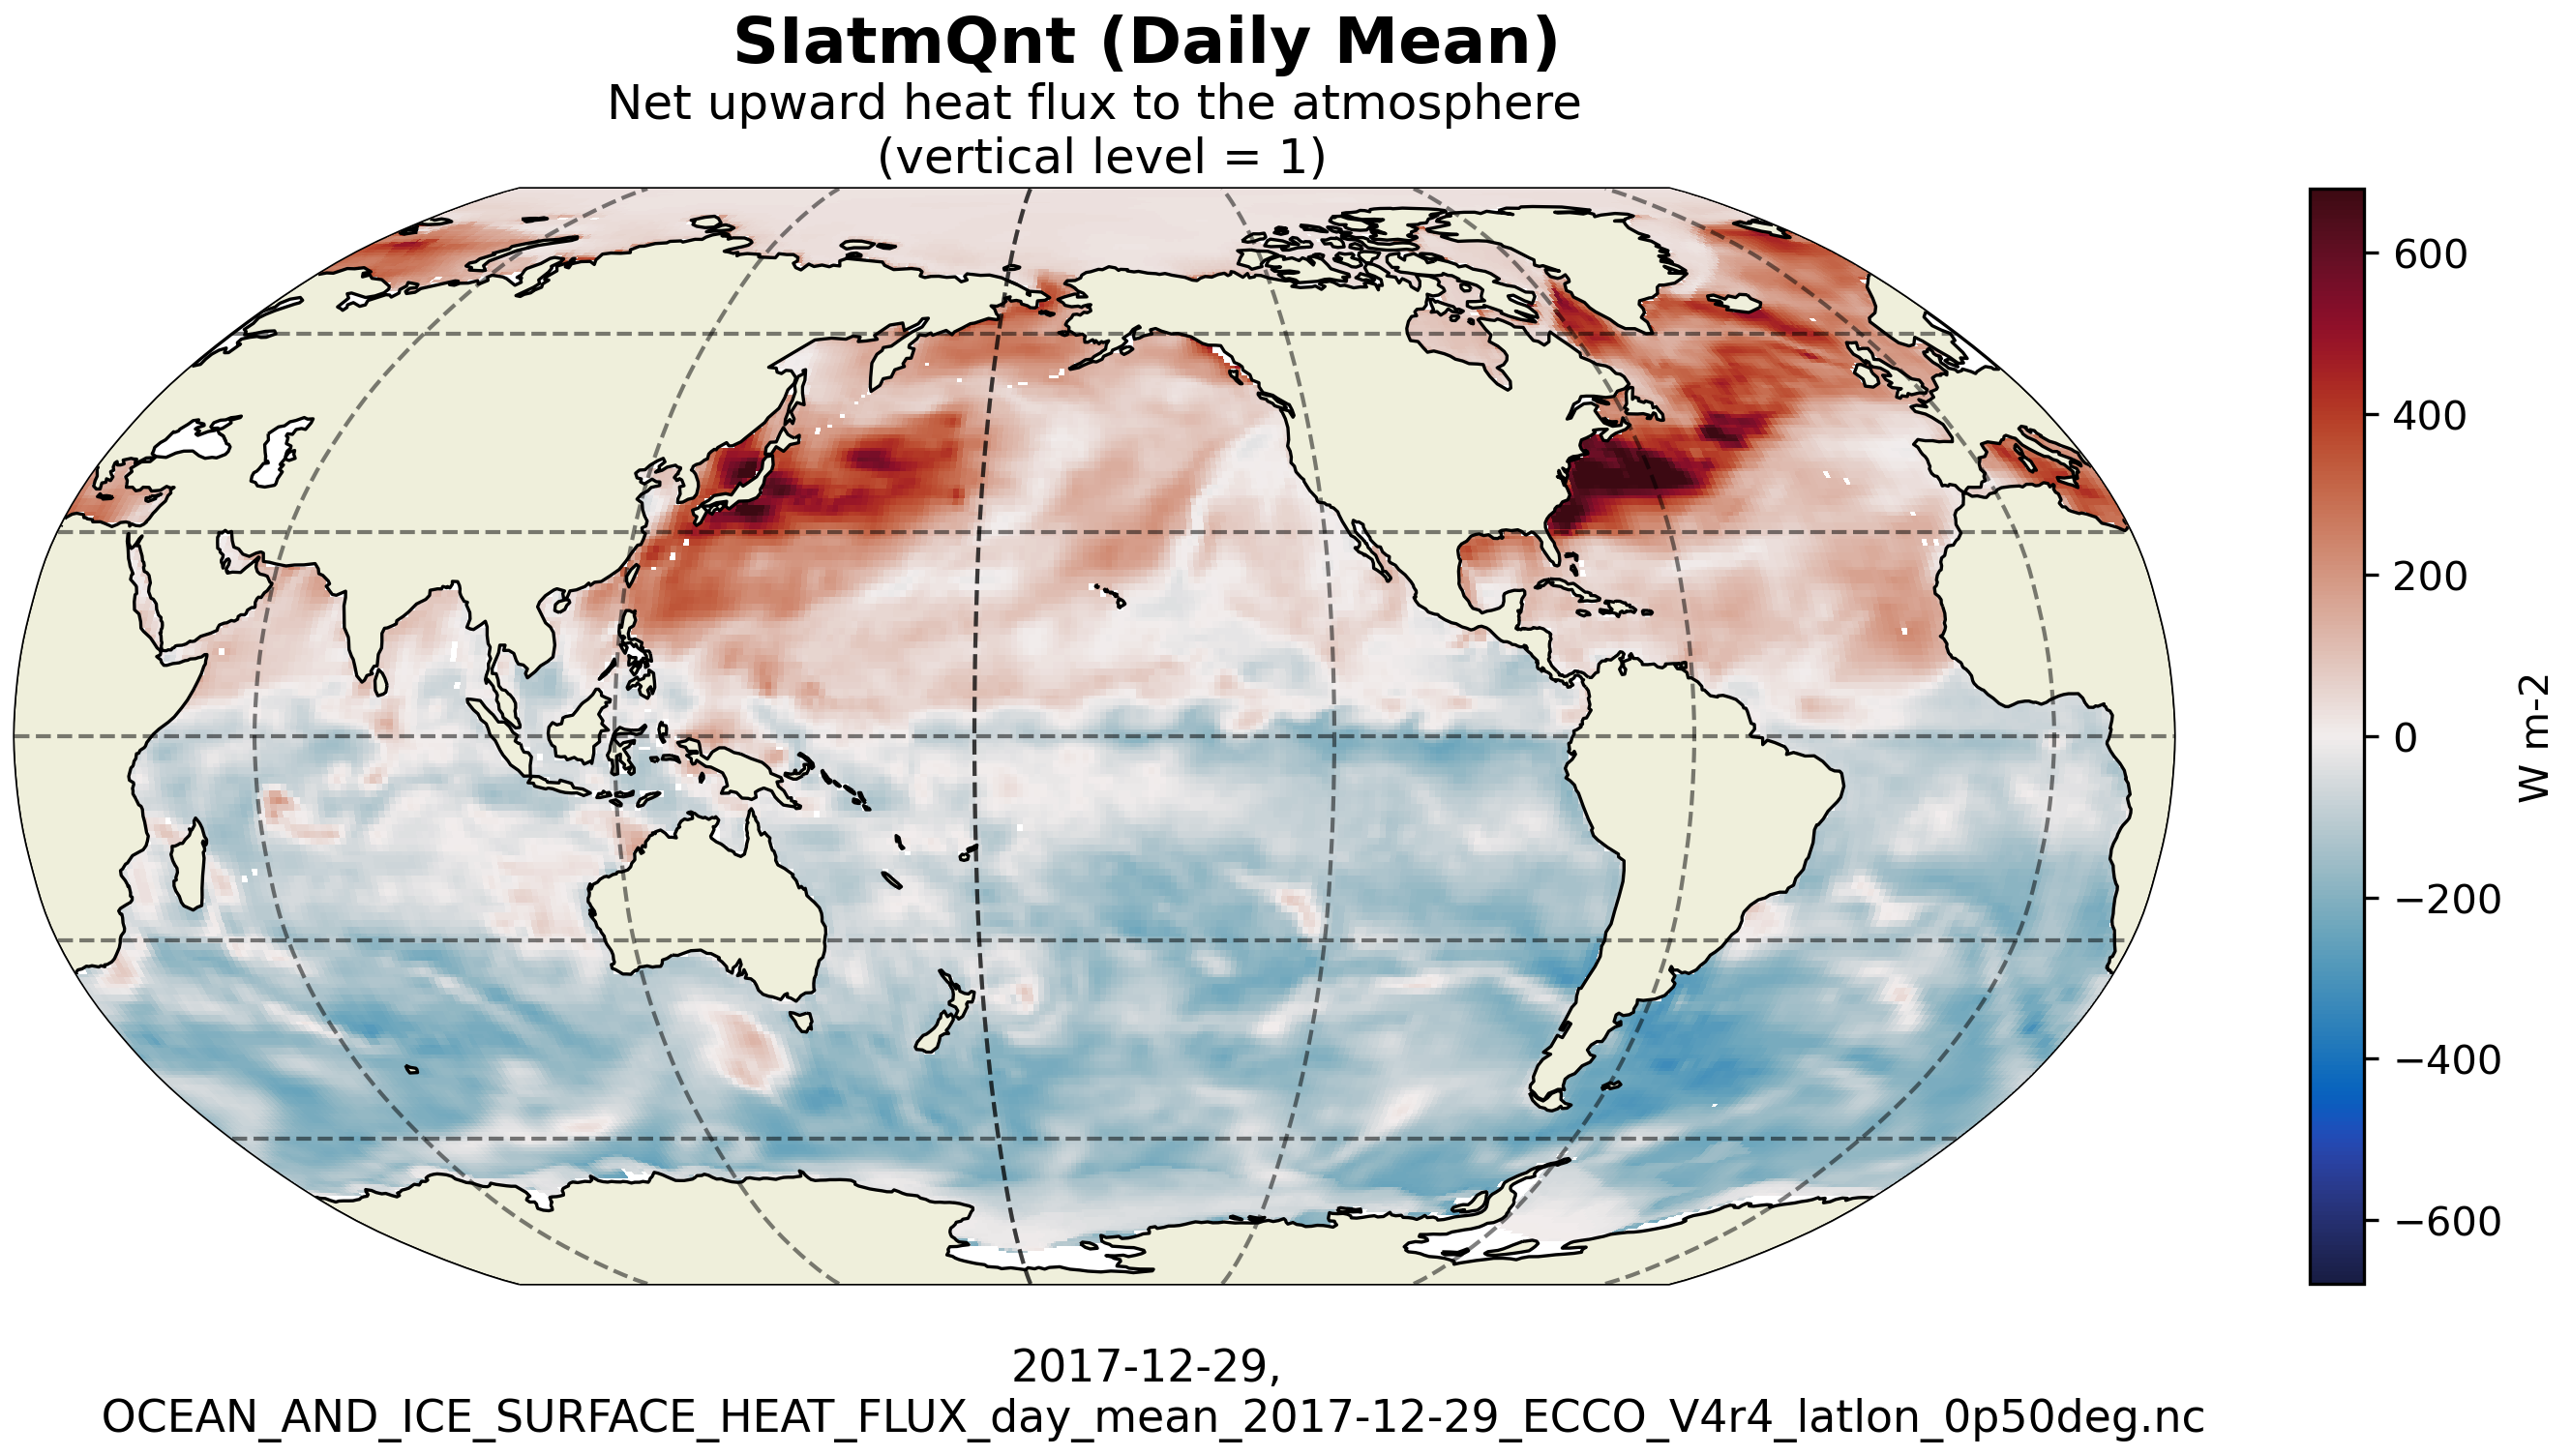
\includegraphics[width=\textwidth]{../images/plots/latlon_plots/Ocean_and_Sea-Ice_Surface_Heat_Fluxes/SIatmQnt.png}
\caption{Dataset: OCEAN\_AND\_ICE\_SURFACE\_HEAT\_FLUX Variable: SIatmQnt}
\label{tab:table-OCEAN_AND_ICE_SURFACE_HEAT_FLUX_SIatmQnt-Plot}
\end{figure}
\pagebreak
\subsubsection{Latlon Variable TFLUX}
\begin{longtable}{|p{0.06\textwidth}|p{0.41\textwidth}|p{0.39\textwidth}|p{0.06\textwidth}|}
\caption{CDL description of OCEAN\_AND\_ICE\_SURFACE\_HEAT\_FLUX's TFLUX variable}
\label{tab:table-OCEAN_AND_ICE_SURFACE_HEAT_FLUX_TFLUX} \\ 
\hline \endhead \hline \endfoot
\rowcolor{lightgray} \textbf{Storage Type} & \textbf{Variable Name} & \textbf{Description} & \textbf{Unit} \\ \hline
float32 & TFLUX & Rate of change of ocean heat content per m2 accounting for mass fluxes. & W m-2 \\ \hline
\rowcolor{lightgray}  \multicolumn{4}{|p{1.00\textwidth}|}{\textbf{CDL Description}} \\ \hline
\multicolumn{4}{|p{1.00\textwidth}|}{\makecell{\parbox{1\textwidth}{float32 TFLUX(time, latitude, longitude)\\
\hspace*{0.5cm}TFLUX: \_FillValue = 9.96921e+36\\
\hspace*{0.5cm}TFLUX: coverage\_content\_type = modelResult\\
\hspace*{0.5cm}TFLUX: direction = >0 increases potential temperature (THETA)\\
\hspace*{0.5cm}TFLUX: long\_name = Rate of change of ocean heat content per m2 accounting for mass fluxes.\\
\hspace*{0.5cm}TFLUX: units = W m: 2\\
\hspace*{0.5cm}TFLUX: coordinates = time\\
\hspace*{0.5cm}TFLUX: valid\_min = : 1713.51220703125\\
\hspace*{0.5cm}TFLUX: valid\_max = 870.3130493164062}}} \\ \hline
\rowcolor{lightgray} \multicolumn{4}{|p{1.00\textwidth}|}{\textbf{Comments}} \\ \hline
\multicolumn{4}{|p{1\textwidth}|}{The rate of change of ocean heat content due to heat fluxes across the liquid surface and the addition or removal of mass. . Note: the global area integral of TFLUX and geothermal flux (geothermalFlux.bin) matches the time-derivative of ocean heat content (J/s). Unlike oceQnet, TFLUX includes the contribution to the ocean heat content from changing ocean mass (e.g. from oceFWflx).} \\ \hline
\end{longtable}

\begin{figure}[H]
\centering
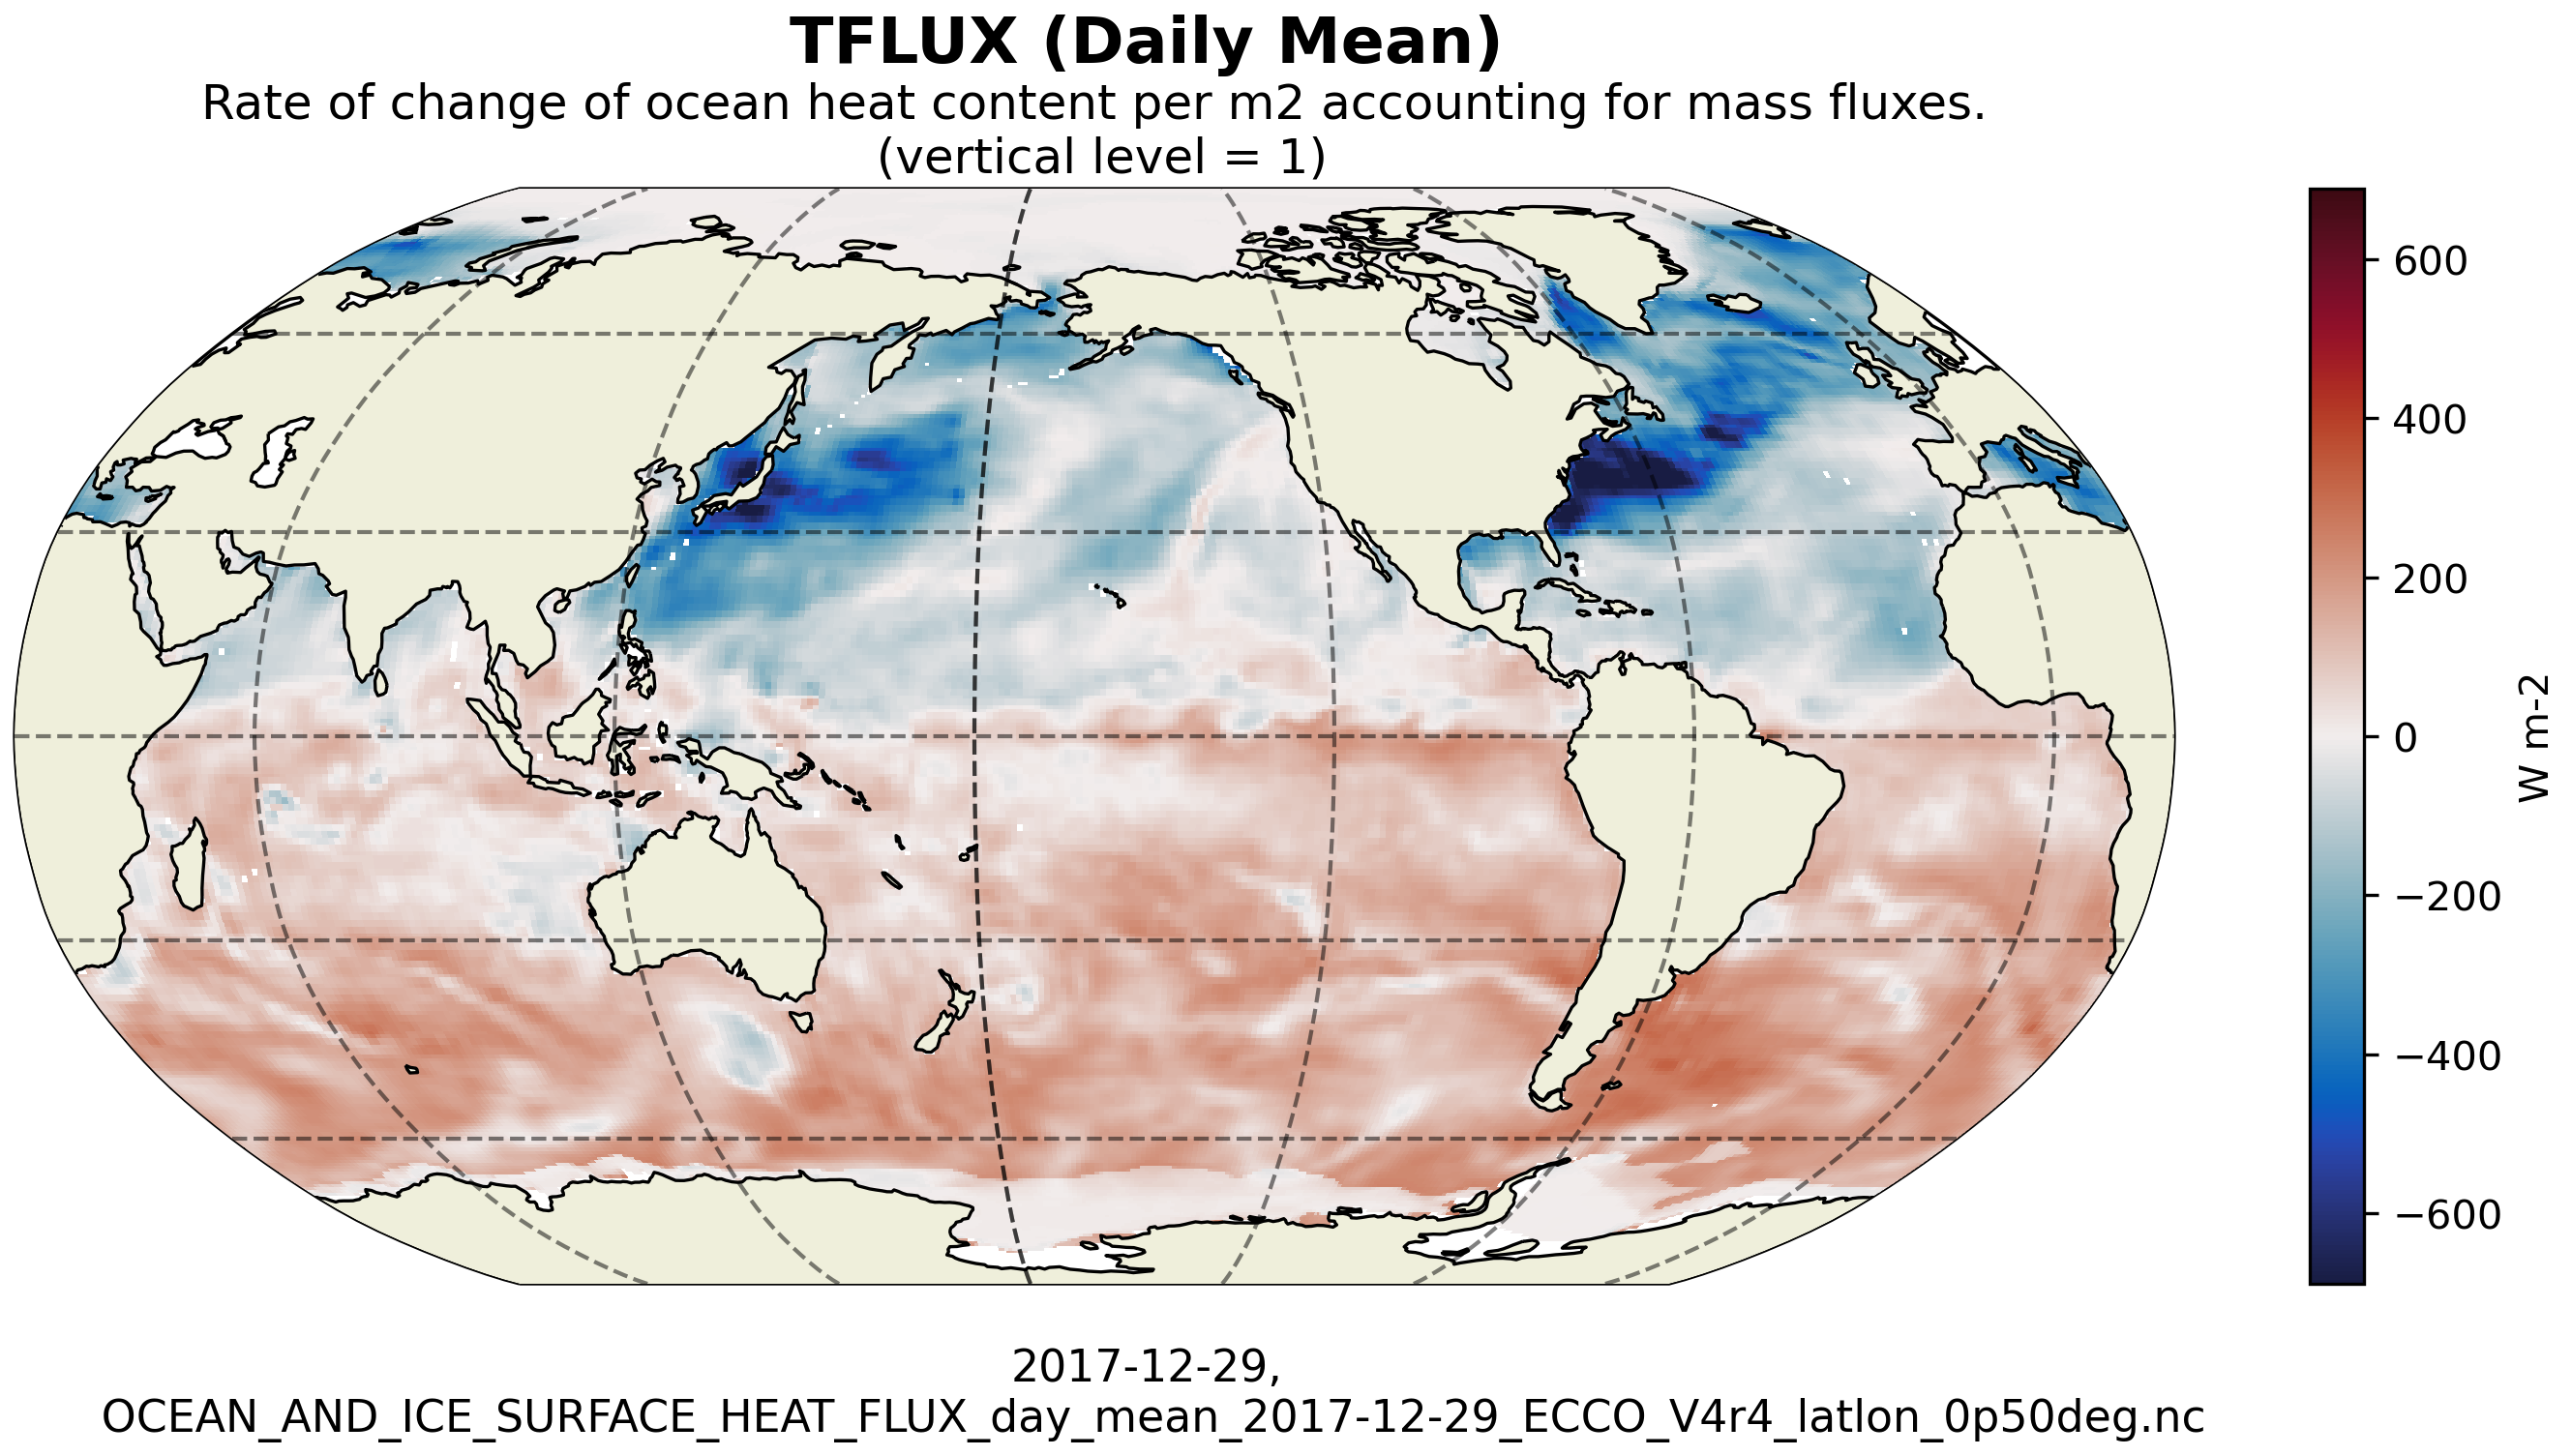
\includegraphics[width=\textwidth]{../images/plots/latlon_plots/Ocean_and_Sea-Ice_Surface_Heat_Fluxes/TFLUX.png}
\caption{Dataset: OCEAN\_AND\_ICE\_SURFACE\_HEAT\_FLUX Variable: TFLUX}
\label{tab:table-OCEAN_AND_ICE_SURFACE_HEAT_FLUX_TFLUX-Plot}
\end{figure}
\pagebreak
\subsubsection{Latlon Variable oceQnet}
\begin{longtable}{|p{0.06\textwidth}|p{0.41\textwidth}|p{0.39\textwidth}|p{0.06\textwidth}|}
\caption{CDL description of OCEAN\_AND\_ICE\_SURFACE\_HEAT\_FLUX's oceQnet variable}
\label{tab:table-OCEAN_AND_ICE_SURFACE_HEAT_FLUX_oceQnet} \\ 
\hline \endhead \hline \endfoot
\rowcolor{lightgray} \textbf{Storage Type} & \textbf{Variable Name} & \textbf{Description} & \textbf{Unit} \\ \hline
float32 & oceQnet & Net heat flux into the ocean surface & W m-2 \\ \hline
\rowcolor{lightgray}  \multicolumn{4}{|p{1.00\textwidth}|}{\textbf{CDL Description}} \\ \hline
\multicolumn{4}{|p{1.00\textwidth}|}{\makecell{\parbox{1\textwidth}{float32 oceQnet(time, latitude, longitude)\\
\hspace*{0.5cm}oceQnet: \_FillValue = 9.96921e+36\\
\hspace*{0.5cm}oceQnet: coverage\_content\_type = modelResult\\
\hspace*{0.5cm}oceQnet: direction = >0 increases potential temperature (THETA)\\
\hspace*{0.5cm}oceQnet: long\_name = Net heat flux into the ocean surface\\
\hspace*{0.5cm}oceQnet: standard\_name = surface\_downward\_heat\_flux\_in\_sea\_water\\
\hspace*{0.5cm}oceQnet: units = W m: 2\\
\hspace*{0.5cm}oceQnet: coordinates = time\\
\hspace*{0.5cm}oceQnet: valid\_min = : 1708.8460693359375\\
\hspace*{0.5cm}oceQnet: valid\_max = 675.3716430664062}}} \\ \hline
\rowcolor{lightgray} \multicolumn{4}{|p{1.00\textwidth}|}{\textbf{Comments}} \\ \hline
\multicolumn{4}{|p{1\textwidth}|}{Net heat flux into the ocean surface from all processes: air-sea turbulent and radiative fluxes and turbulent and conductive fluxes between the ocean and sea-ice and snow. Note: oceQnet does not include the change in ocean heat content due to changing ocean ocean mass (oceFWflx). Mass fluxes from evaporation, precipitation, and runoff (EXFempmr) happen at the same temperature as the ocean surface temperature. Consequently, EmPmR does not change ocean surface temperature. Conversely, mass fluxes due to sea-ice thickening/thinning and snow melt in the model are assumed to happen at a fixed 0C. Consequently, mass fluxes due to phase changes between seawater and sea-ice and snow induce a heat flux when the ocean surface temperaure is not 0C. The variable TFLUX does include the change in ocean heat content due to changing ocean mass.} \\ \hline
\end{longtable}

\begin{figure}[H]
\centering
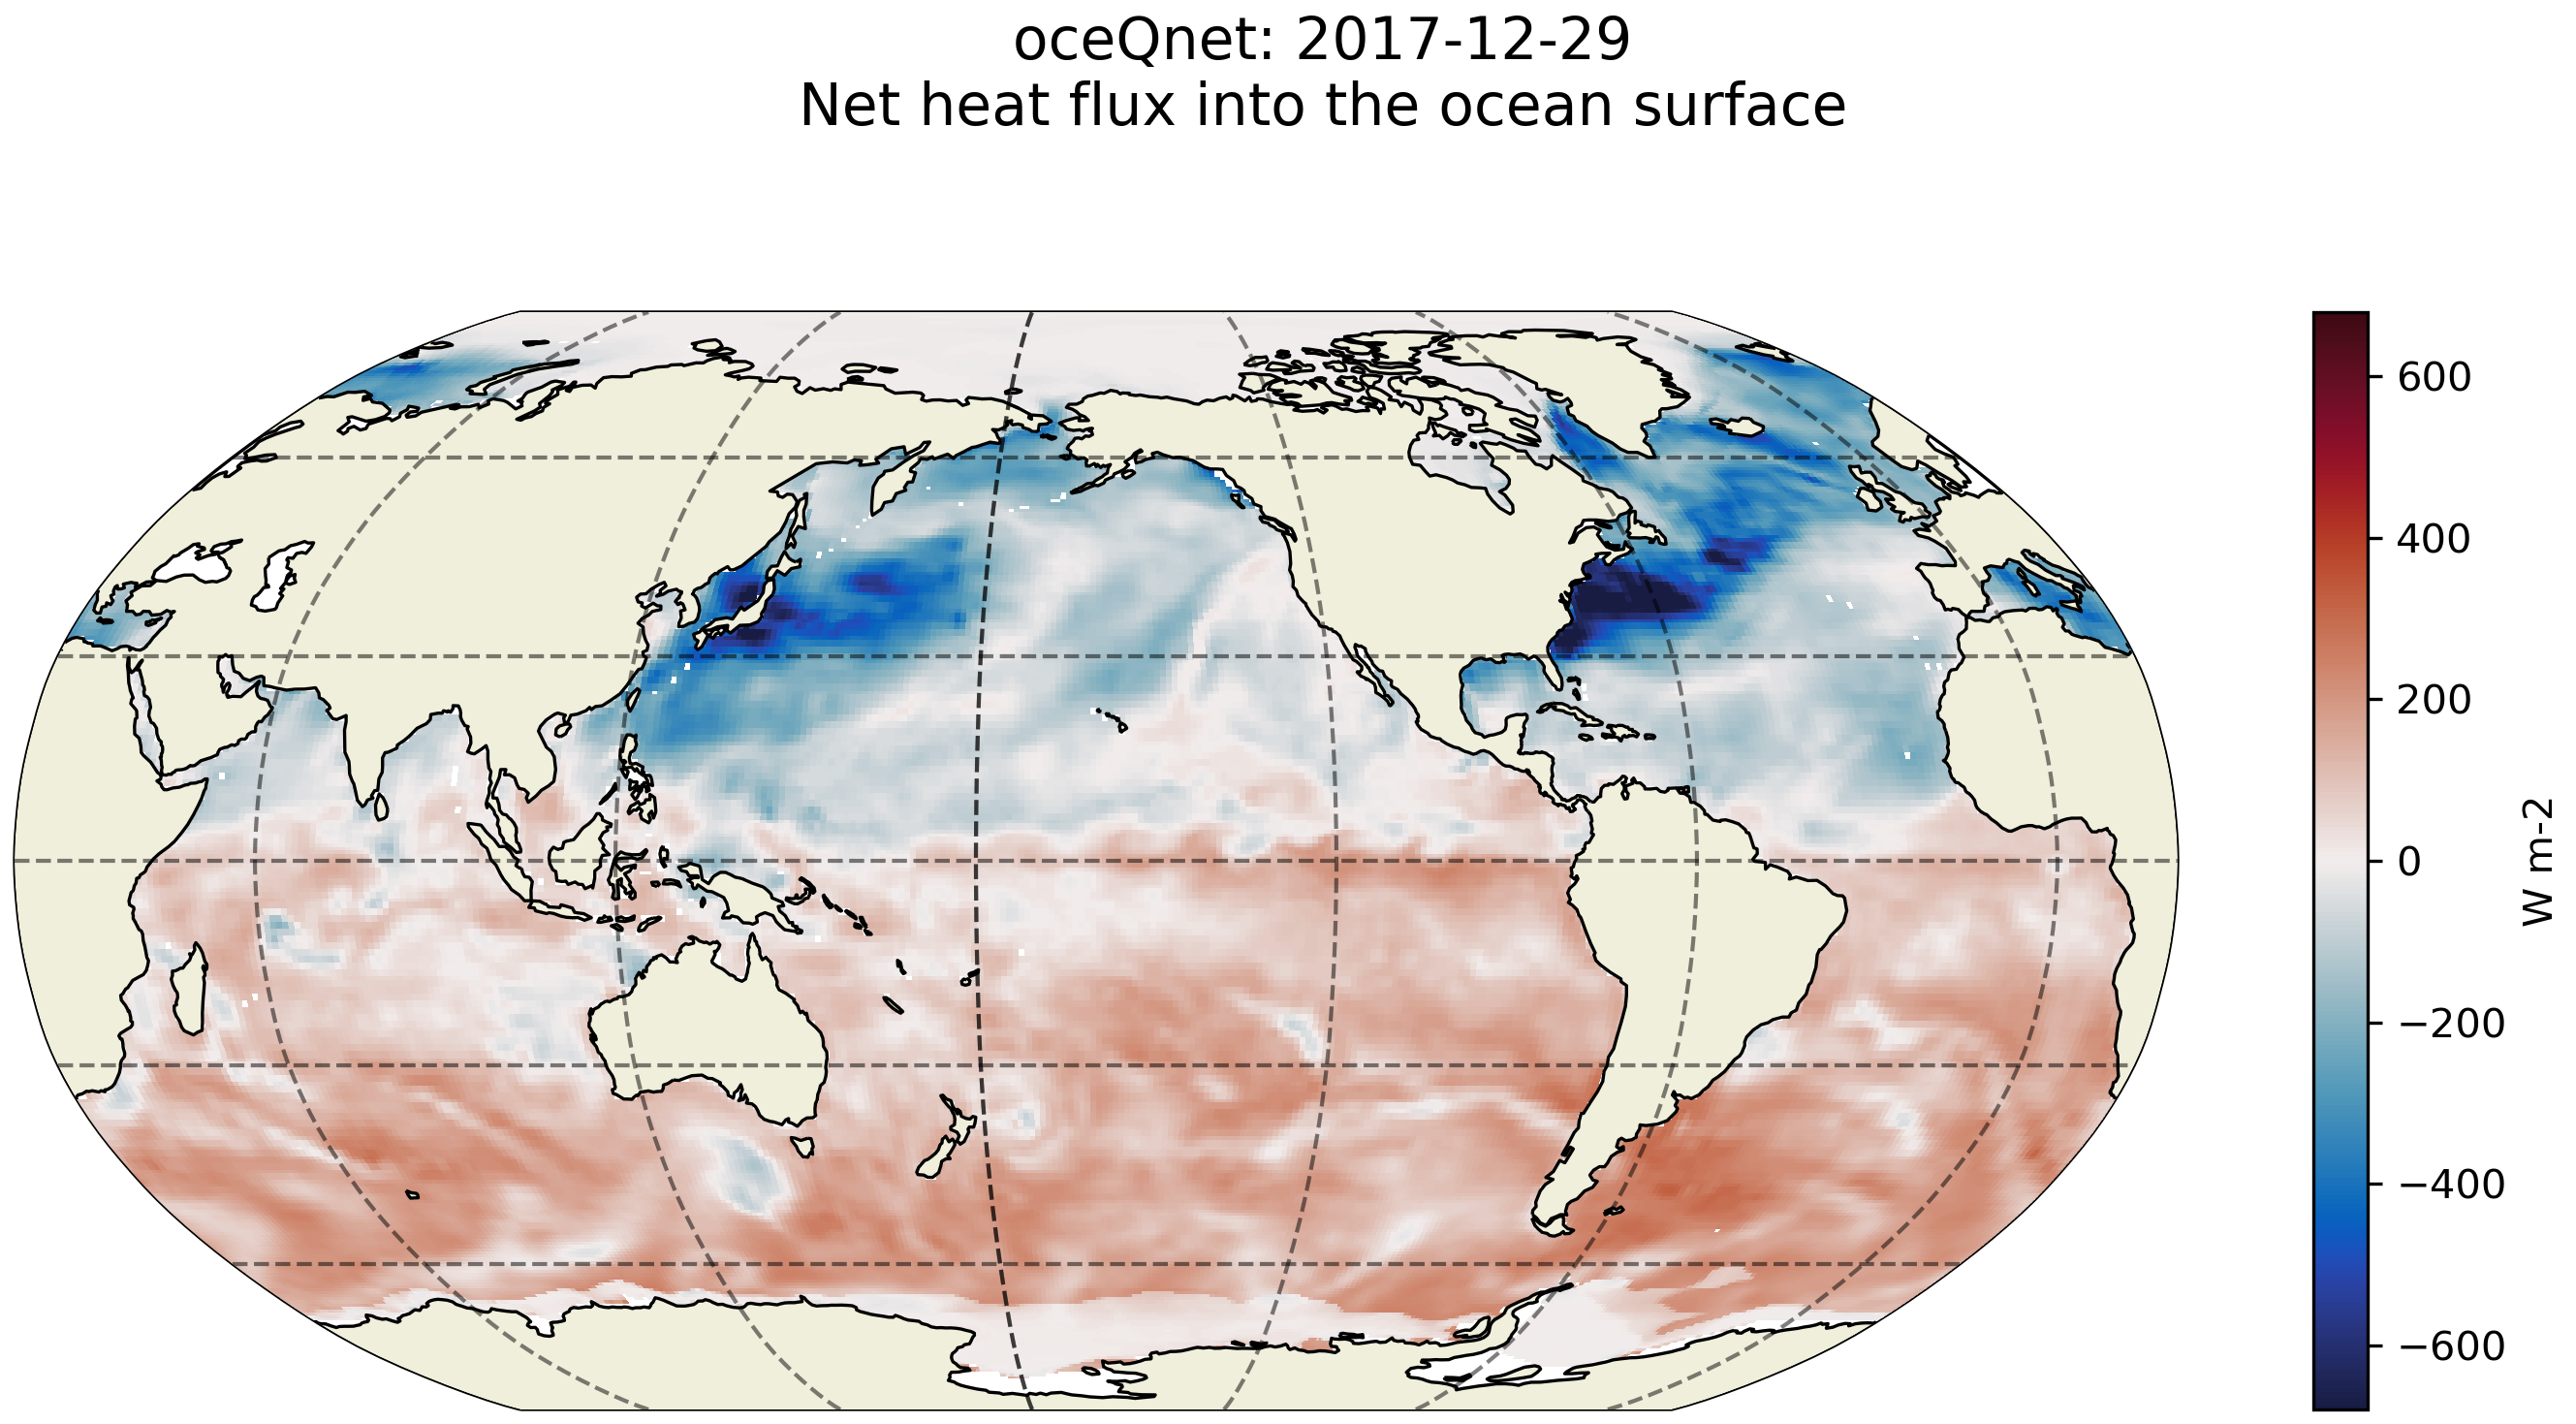
\includegraphics[width=\textwidth]{../images/plots/latlon_plots/Ocean_and_Sea-Ice_Surface_Heat_Fluxes/oceQnet.png}
\caption{Dataset: OCEAN\_AND\_ICE\_SURFACE\_HEAT\_FLUX Variable: oceQnet}
\label{tab:table-OCEAN_AND_ICE_SURFACE_HEAT_FLUX_oceQnet-Plot}
\end{figure}
\pagebreak
\subsubsection{Latlon Variable oceQsw}
\begin{longtable}{|p{0.06\textwidth}|p{0.41\textwidth}|p{0.39\textwidth}|p{0.06\textwidth}|}
\caption{CDL description of OCEAN\_AND\_ICE\_SURFACE\_HEAT\_FLUX's oceQsw variable}
\label{tab:table-OCEAN_AND_ICE_SURFACE_HEAT_FLUX_oceQsw} \\ 
\hline \endhead \hline \endfoot
\rowcolor{lightgray} \textbf{Storage Type} & \textbf{Variable Name} & \textbf{Description} & \textbf{Unit} \\ \hline
float32 & oceQsw & Net shortwave radiative flux across the ocean surface & W m-2 \\ \hline
\rowcolor{lightgray}  \multicolumn{4}{|p{1.00\textwidth}|}{\textbf{CDL Description}} \\ \hline
\multicolumn{4}{|p{1.00\textwidth}|}{\makecell{\parbox{1\textwidth}{float32 oceQsw(time, latitude, longitude)\\
\hspace*{0.5cm}oceQsw: \_FillValue = 9.96921e+36\\
\hspace*{0.5cm}oceQsw: coverage\_content\_type = modelResult\\
\hspace*{0.5cm}oceQsw: direction = >0 increases potential temperature (THETA)\\
\hspace*{0.5cm}oceQsw: long\_name = Net shortwave radiative flux across the ocean surface\\
\hspace*{0.5cm}oceQsw: units = W m: 2\\
\hspace*{0.5cm}oceQsw: coordinates = time\\
\hspace*{0.5cm}oceQsw: valid\_min = : 134.39808654785156\\
\hspace*{0.5cm}oceQsw: valid\_max = 655.6171264648438}}} \\ \hline
\rowcolor{lightgray} \multicolumn{4}{|p{1.00\textwidth}|}{\textbf{Comments}} \\ \hline
\multicolumn{4}{|p{1\textwidth}|}{Net shortwave radiative flux across the ocean surface. Note: Shortwave radiation penetrates below the surface grid cell.} \\ \hline
\end{longtable}

\begin{figure}[H]
\centering
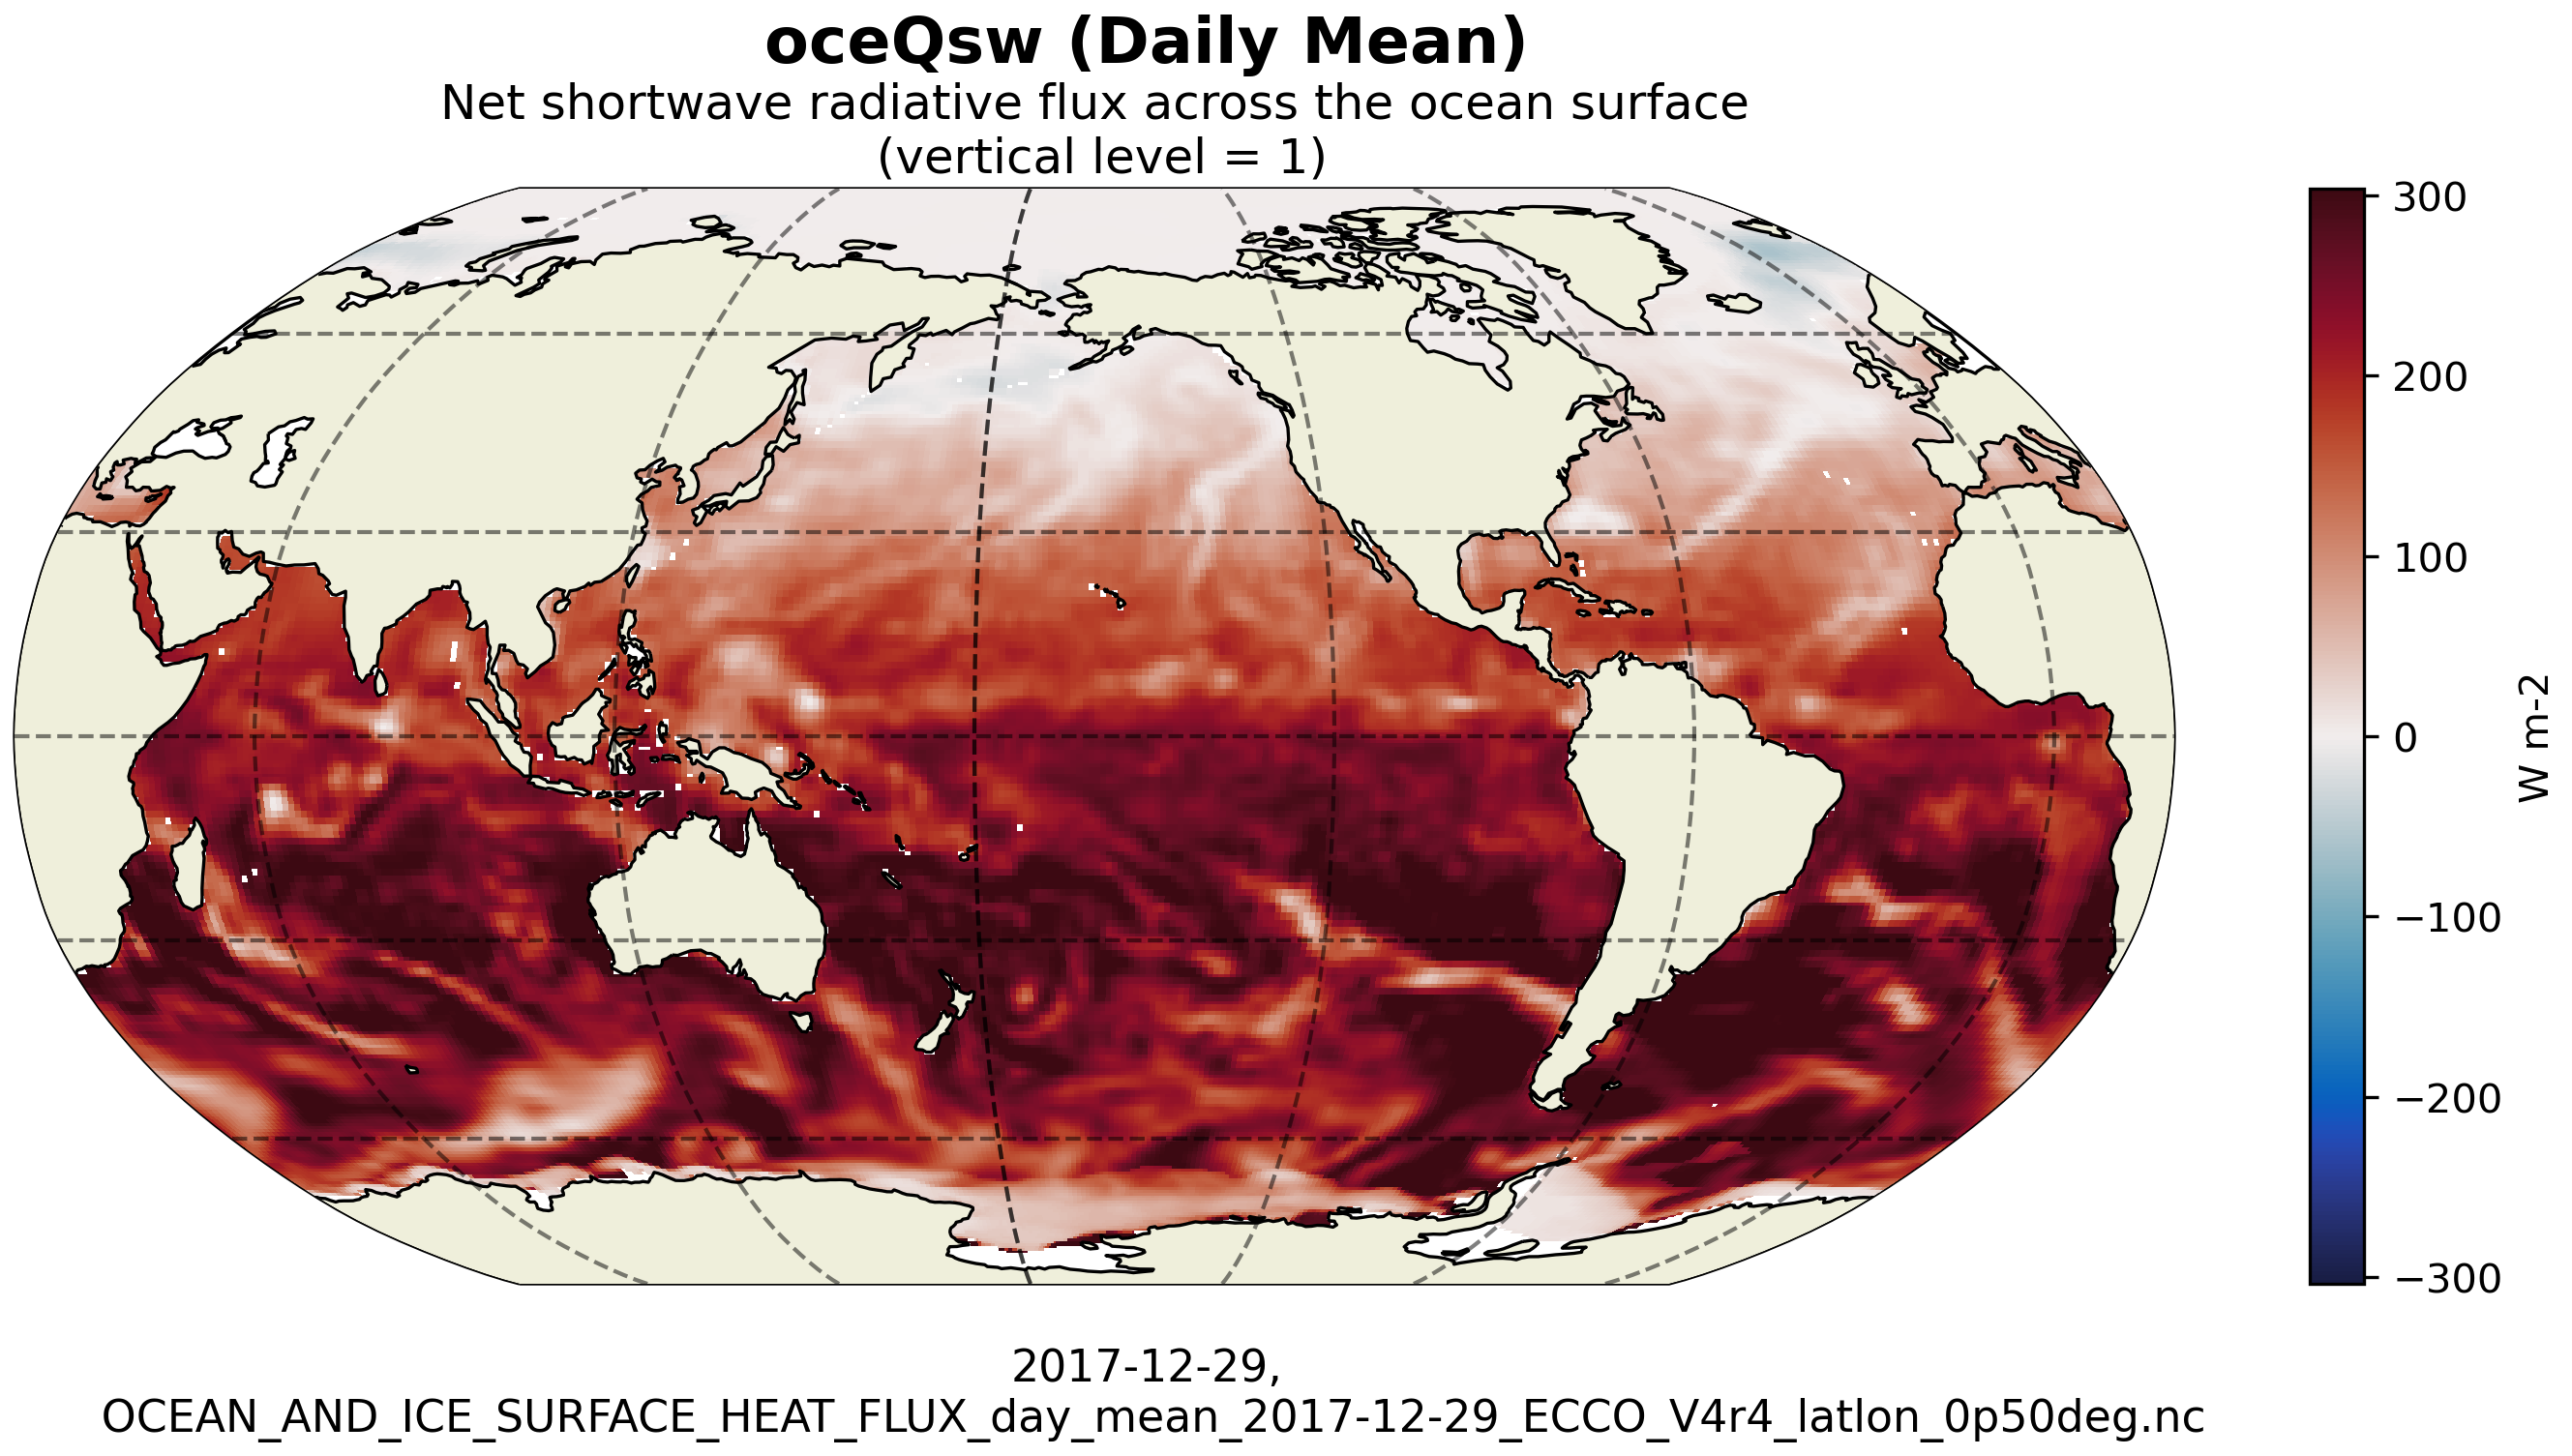
\includegraphics[width=\textwidth]{../images/plots/latlon_plots/Ocean_and_Sea-Ice_Surface_Heat_Fluxes/oceQsw.png}
\caption{Dataset: OCEAN\_AND\_ICE\_SURFACE\_HEAT\_FLUX Variable: oceQsw}
\label{tab:table-OCEAN_AND_ICE_SURFACE_HEAT_FLUX_oceQsw-Plot}
\end{figure}
\pagebreak
\subsection{Latlon NetCDF OCEAN\_AND\_ICE\_SURFACE\_STRESS}
\newp
\begin{longtable}{|p{0.1\textwidth}|p{0.5\textwidth}|}
\caption{Variables in the dataset OCEAN\_AND\_ICE\_SURFACE\_STRESS}
\label{tab:table-OCEAN_AND_ICE_SURFACE_STRESS-fields} \\ 
\hline \endhead \hline \endfoot
\rowcolor{lightgray} \textbf{Dataset:} & \textbf{OCEAN\_AND\_ICE\_SURFACE\_STRESS} \\ \hline
Field: &EXFtaue \\ \hline
Field: &EXFtaun \\ \hline
Field: &oceTAUE \\ \hline
Field: &oceTAUN \\ \hline
\end{longtable}

\pagebreak
\subsubsection{Latlon Variable EXFtaue}
\begin{longtable}{|p{0.06\textwidth}|p{0.41\textwidth}|p{0.39\textwidth}|p{0.06\textwidth}|}
\caption{CDL description of OCEAN\_AND\_ICE\_SURFACE\_STRESS's EXFtaue variable}
\label{tab:table-OCEAN_AND_ICE_SURFACE_STRESS_EXFtaue} \\ 
\hline \endhead \hline \endfoot
\rowcolor{lightgray} \textbf{Storage Type} & \textbf{Variable Name} & \textbf{Description} & \textbf{Unit} \\ \hline
float32 & EXFtaue & Zonal (east-west) wind stress & N m-2 \\ \hline
\rowcolor{lightgray}  \multicolumn{4}{|p{1.00\textwidth}|}{\textbf{CDL Description}} \\ \hline
\multicolumn{4}{|p{1.00\textwidth}|}{\makecell{\parbox{1\textwidth}{float32 EXFtaue(time, latitude, longitude)\\
\hspace*{0.5cm}EXFtaue: \_FillValue = 9.96921e+36\\
\hspace*{0.5cm}EXFtaue: coverage\_content\_type = modelResult\\
\hspace*{0.5cm}EXFtaue: direction =  >0 increases eastward velocity (EVEL)\\
\hspace*{0.5cm}EXFtaue: long\_name = Zonal (east: west) wind stress\\
\hspace*{0.5cm}EXFtaue: standard\_name = surface\_downward\_eastward\_stress\\
\hspace*{0.5cm}EXFtaue: units = N m: 2\\
\hspace*{0.5cm}EXFtaue: coordinates = time\\
\hspace*{0.5cm}EXFtaue: valid\_min = : 3.1686902046203613\\
\hspace*{0.5cm}EXFtaue: valid\_max = 3.284827709197998}}} \\ \hline
\rowcolor{lightgray} \multicolumn{4}{|p{1.00\textwidth}|}{\textbf{Comments}} \\ \hline
\multicolumn{4}{|p{1\textwidth}|}{Zonal (east-west) component of wind stress. Note: EXFtaue is the zonal wind stress applied to the ocean and sea-ice. When sea-ice is present, the total zonal stress applied to the ocean surface is NOT EXFtaue, but a combination of the wind stress in the open water fraction (EXFtaue) and a stress from sea-ice in the ice-covered fraction (see oceTAUE). EXFtaue is calculated by interpolating the model's x and y components of wind stress (EXFtaux and EXFtauy) to tracer cell centers and then finding the zonal component of the interpolated vectors. It is NOT recommended to use EXFtaue and EXFtaun for momentum budget calculations because interpolating EXFtaux and EXFtauy from the model grid to the lat-lon grid introduces errors. For momentum fluxes to the ocean surface see oceTAUx and oceTAUy.} \\ \hline
\end{longtable}

\begin{figure}[H]
\centering
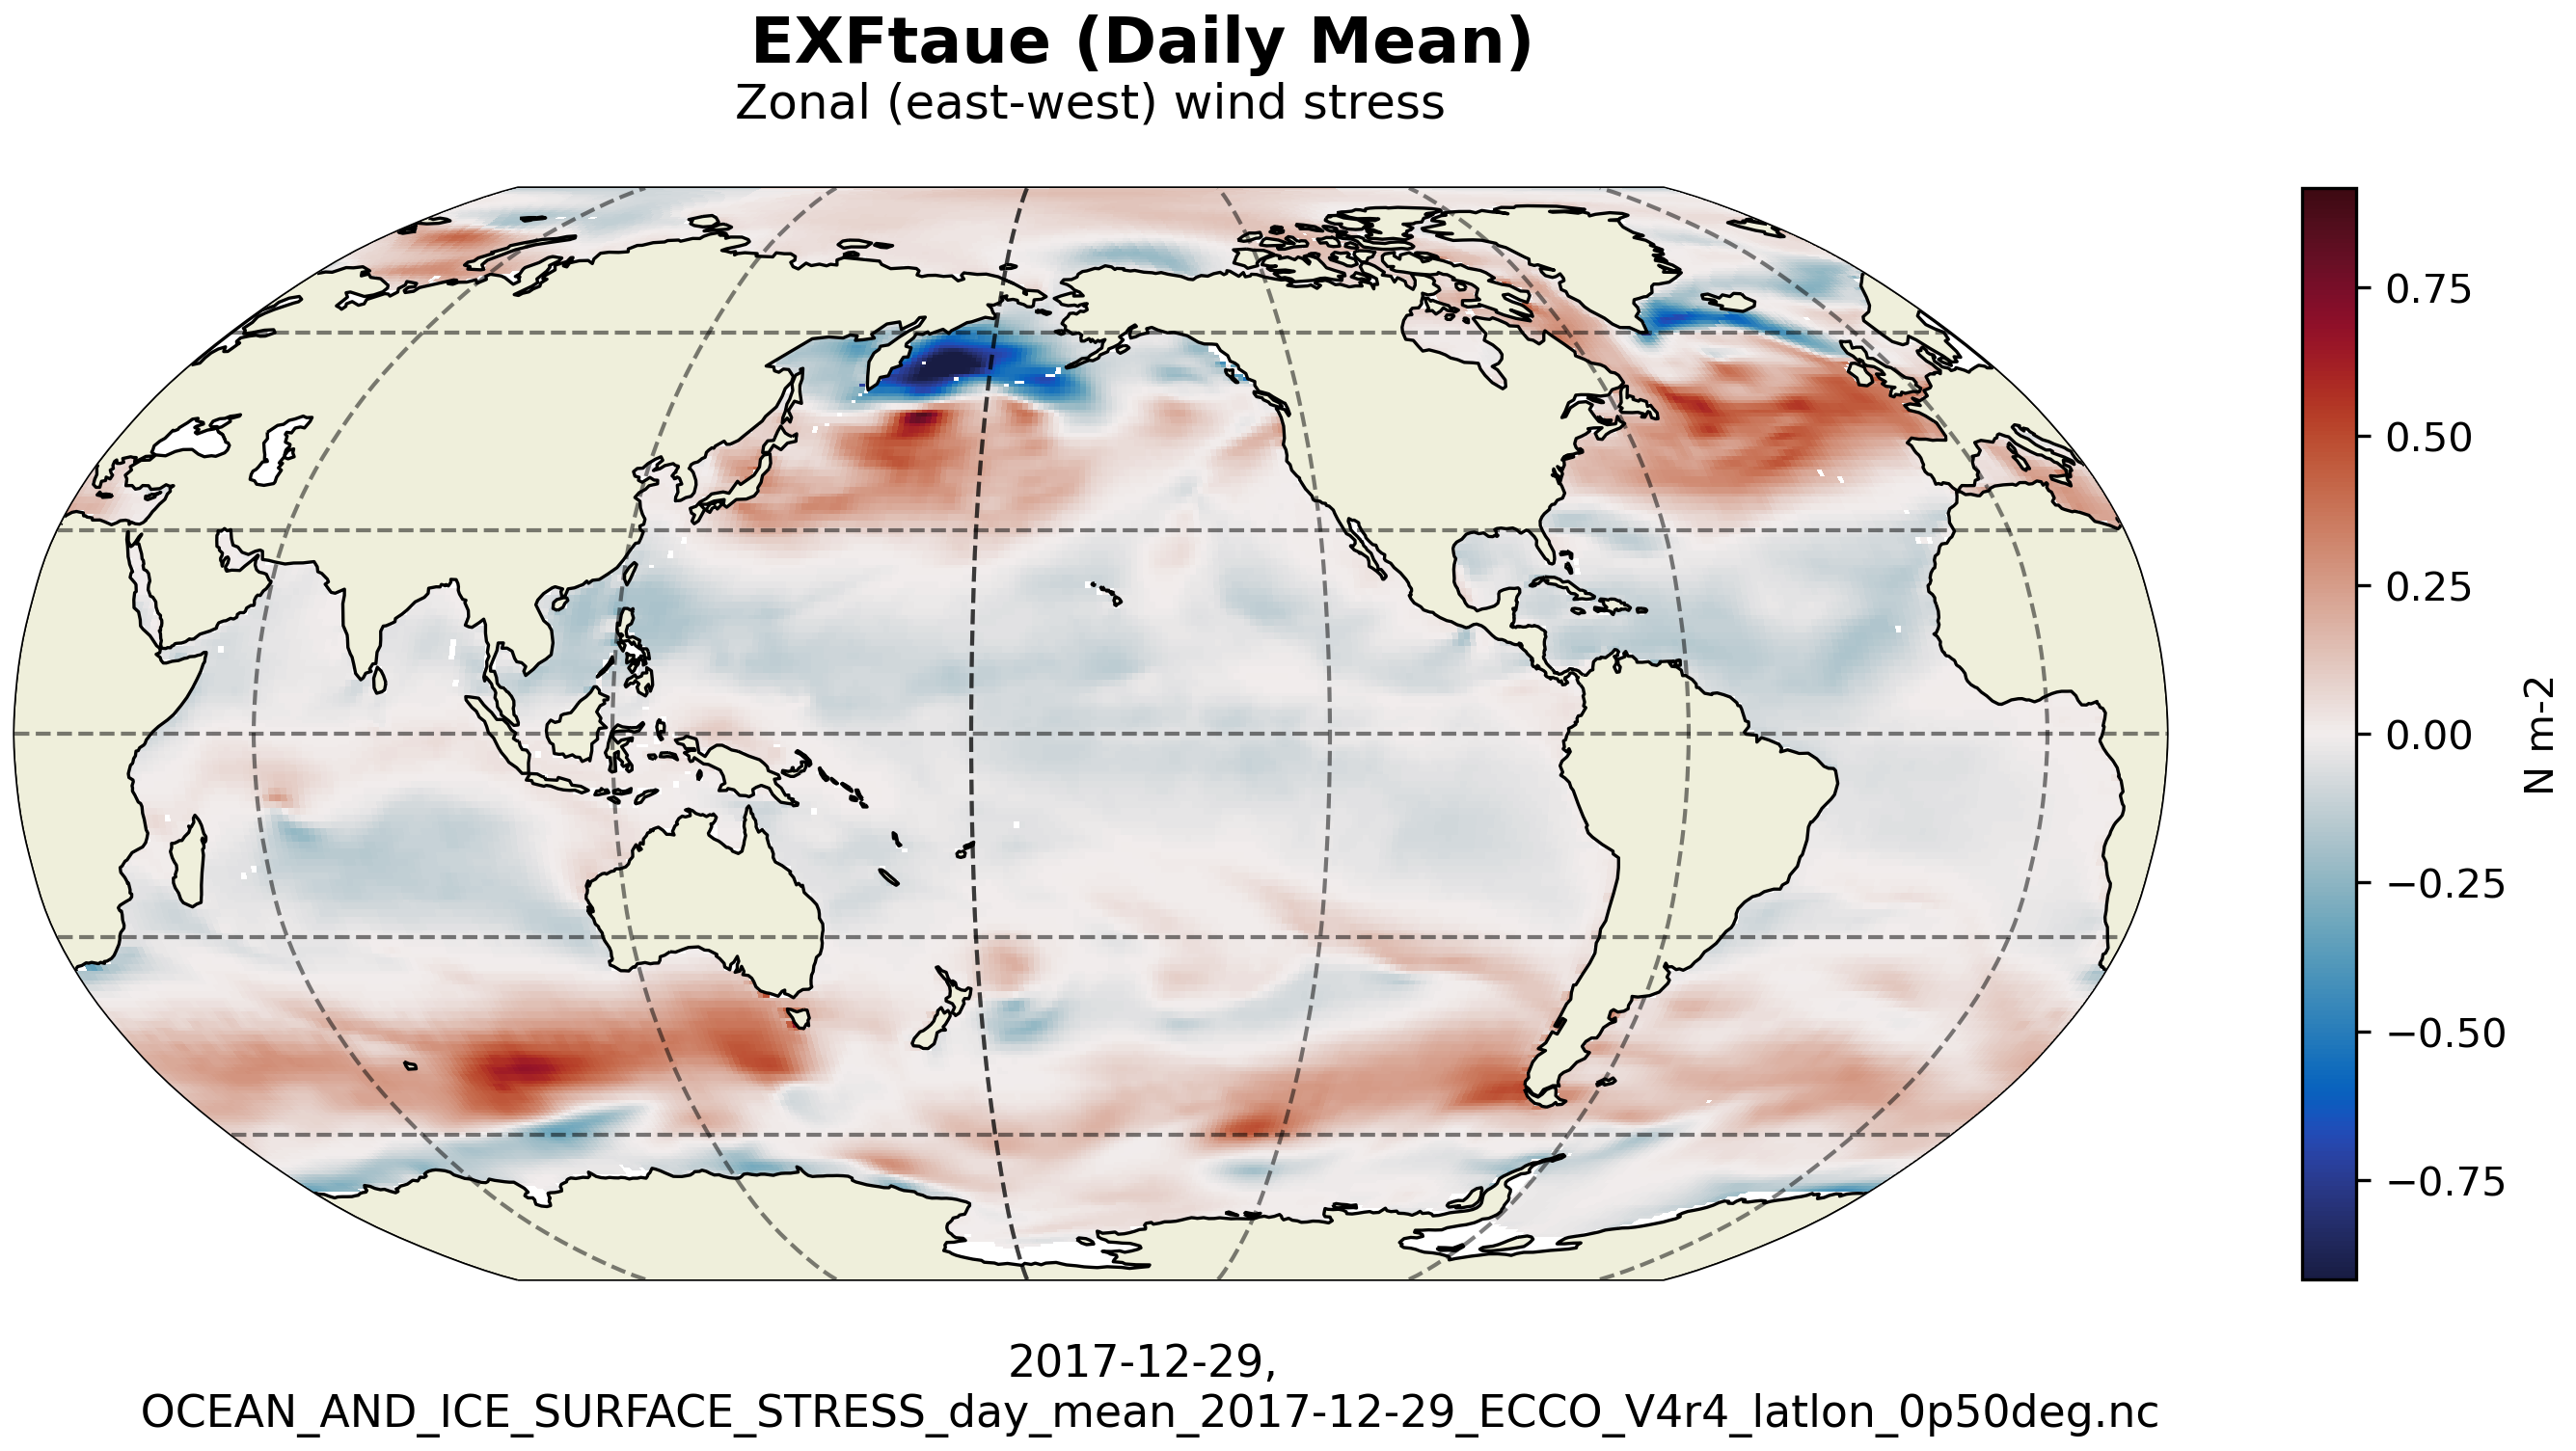
\includegraphics[width=\textwidth]{../images/plots/latlon_plots/Ocean_and_Sea-Ice_Surface_Stress/EXFtaue.png}
\caption{Dataset: OCEAN\_AND\_ICE\_SURFACE\_STRESS Variable: EXFtaue}
\label{tab:table-OCEAN_AND_ICE_SURFACE_STRESS_EXFtaue-Plot}
\end{figure}
\pagebreak
\subsubsection{Latlon Variable EXFtaun}
\begin{longtable}{|p{0.06\textwidth}|p{0.41\textwidth}|p{0.39\textwidth}|p{0.06\textwidth}|}
\caption{CDL description of OCEAN\_AND\_ICE\_SURFACE\_STRESS's EXFtaun variable}
\label{tab:table-OCEAN_AND_ICE_SURFACE_STRESS_EXFtaun} \\ 
\hline \endhead \hline \endfoot
\rowcolor{lightgray} \textbf{Storage Type} & \textbf{Variable Name} & \textbf{Description} & \textbf{Unit} \\ \hline
float32 & EXFtaun & Meridional (north-south) wind stress & N m-2 \\ \hline
\rowcolor{lightgray}  \multicolumn{4}{|p{1.00\textwidth}|}{\textbf{CDL Description}} \\ \hline
\multicolumn{4}{|p{1.00\textwidth}|}{\makecell{\parbox{1\textwidth}{float32 EXFtaun(time, latitude, longitude)\\
\hspace*{0.5cm}EXFtaun: \_FillValue = 9.96921e+36\\
\hspace*{0.5cm}EXFtaun: coverage\_content\_type = modelResult\\
\hspace*{0.5cm}EXFtaun: direction =  >0 increases northward velocity (NVEL)\\
\hspace*{0.5cm}EXFtaun: long\_name = Meridional (north: south) wind stress\\
\hspace*{0.5cm}EXFtaun: standard\_name = surface\_downward\_northward\_stress\\
\hspace*{0.5cm}EXFtaun: units = N m: 2\\
\hspace*{0.5cm}EXFtaun: coordinates = time\\
\hspace*{0.5cm}EXFtaun: valid\_min = : 4.111213207244873\\
\hspace*{0.5cm}EXFtaun: valid\_max = 6.878159523010254}}} \\ \hline
\rowcolor{lightgray} \multicolumn{4}{|p{1.00\textwidth}|}{\textbf{Comments}} \\ \hline
\multicolumn{4}{|p{1\textwidth}|}{Meridional (north-south) component of wind stress. Note: EXFtaun is the stress applied to the ocean and sea-ice. When sea-ice is present, the total meridional stress applied to the ocean surface is NOT EXFtaun, but a combination of the wind stress in the open water fraction (EXFtaun) and a stress from sea-ice in the ice-covered fraction (see oceTAUN).  EXFtaun is calculated by interpolating the model's x and y components of wind stress (EXFtaux and EXFtauy) to tracer cell centers and then determining the meridional component of the interpolated vectors. It is NOT recommended to use EXFtaue and EXFtaun for momentum budget calculations because interpolating EXFtaux and EXFtauy from the model grid to the lat-lon grid introduces errors. For momentum fluxes to the ocean surface see oceTAUx and oceTAUy.} \\ \hline
\end{longtable}

\begin{figure}[H]
\centering
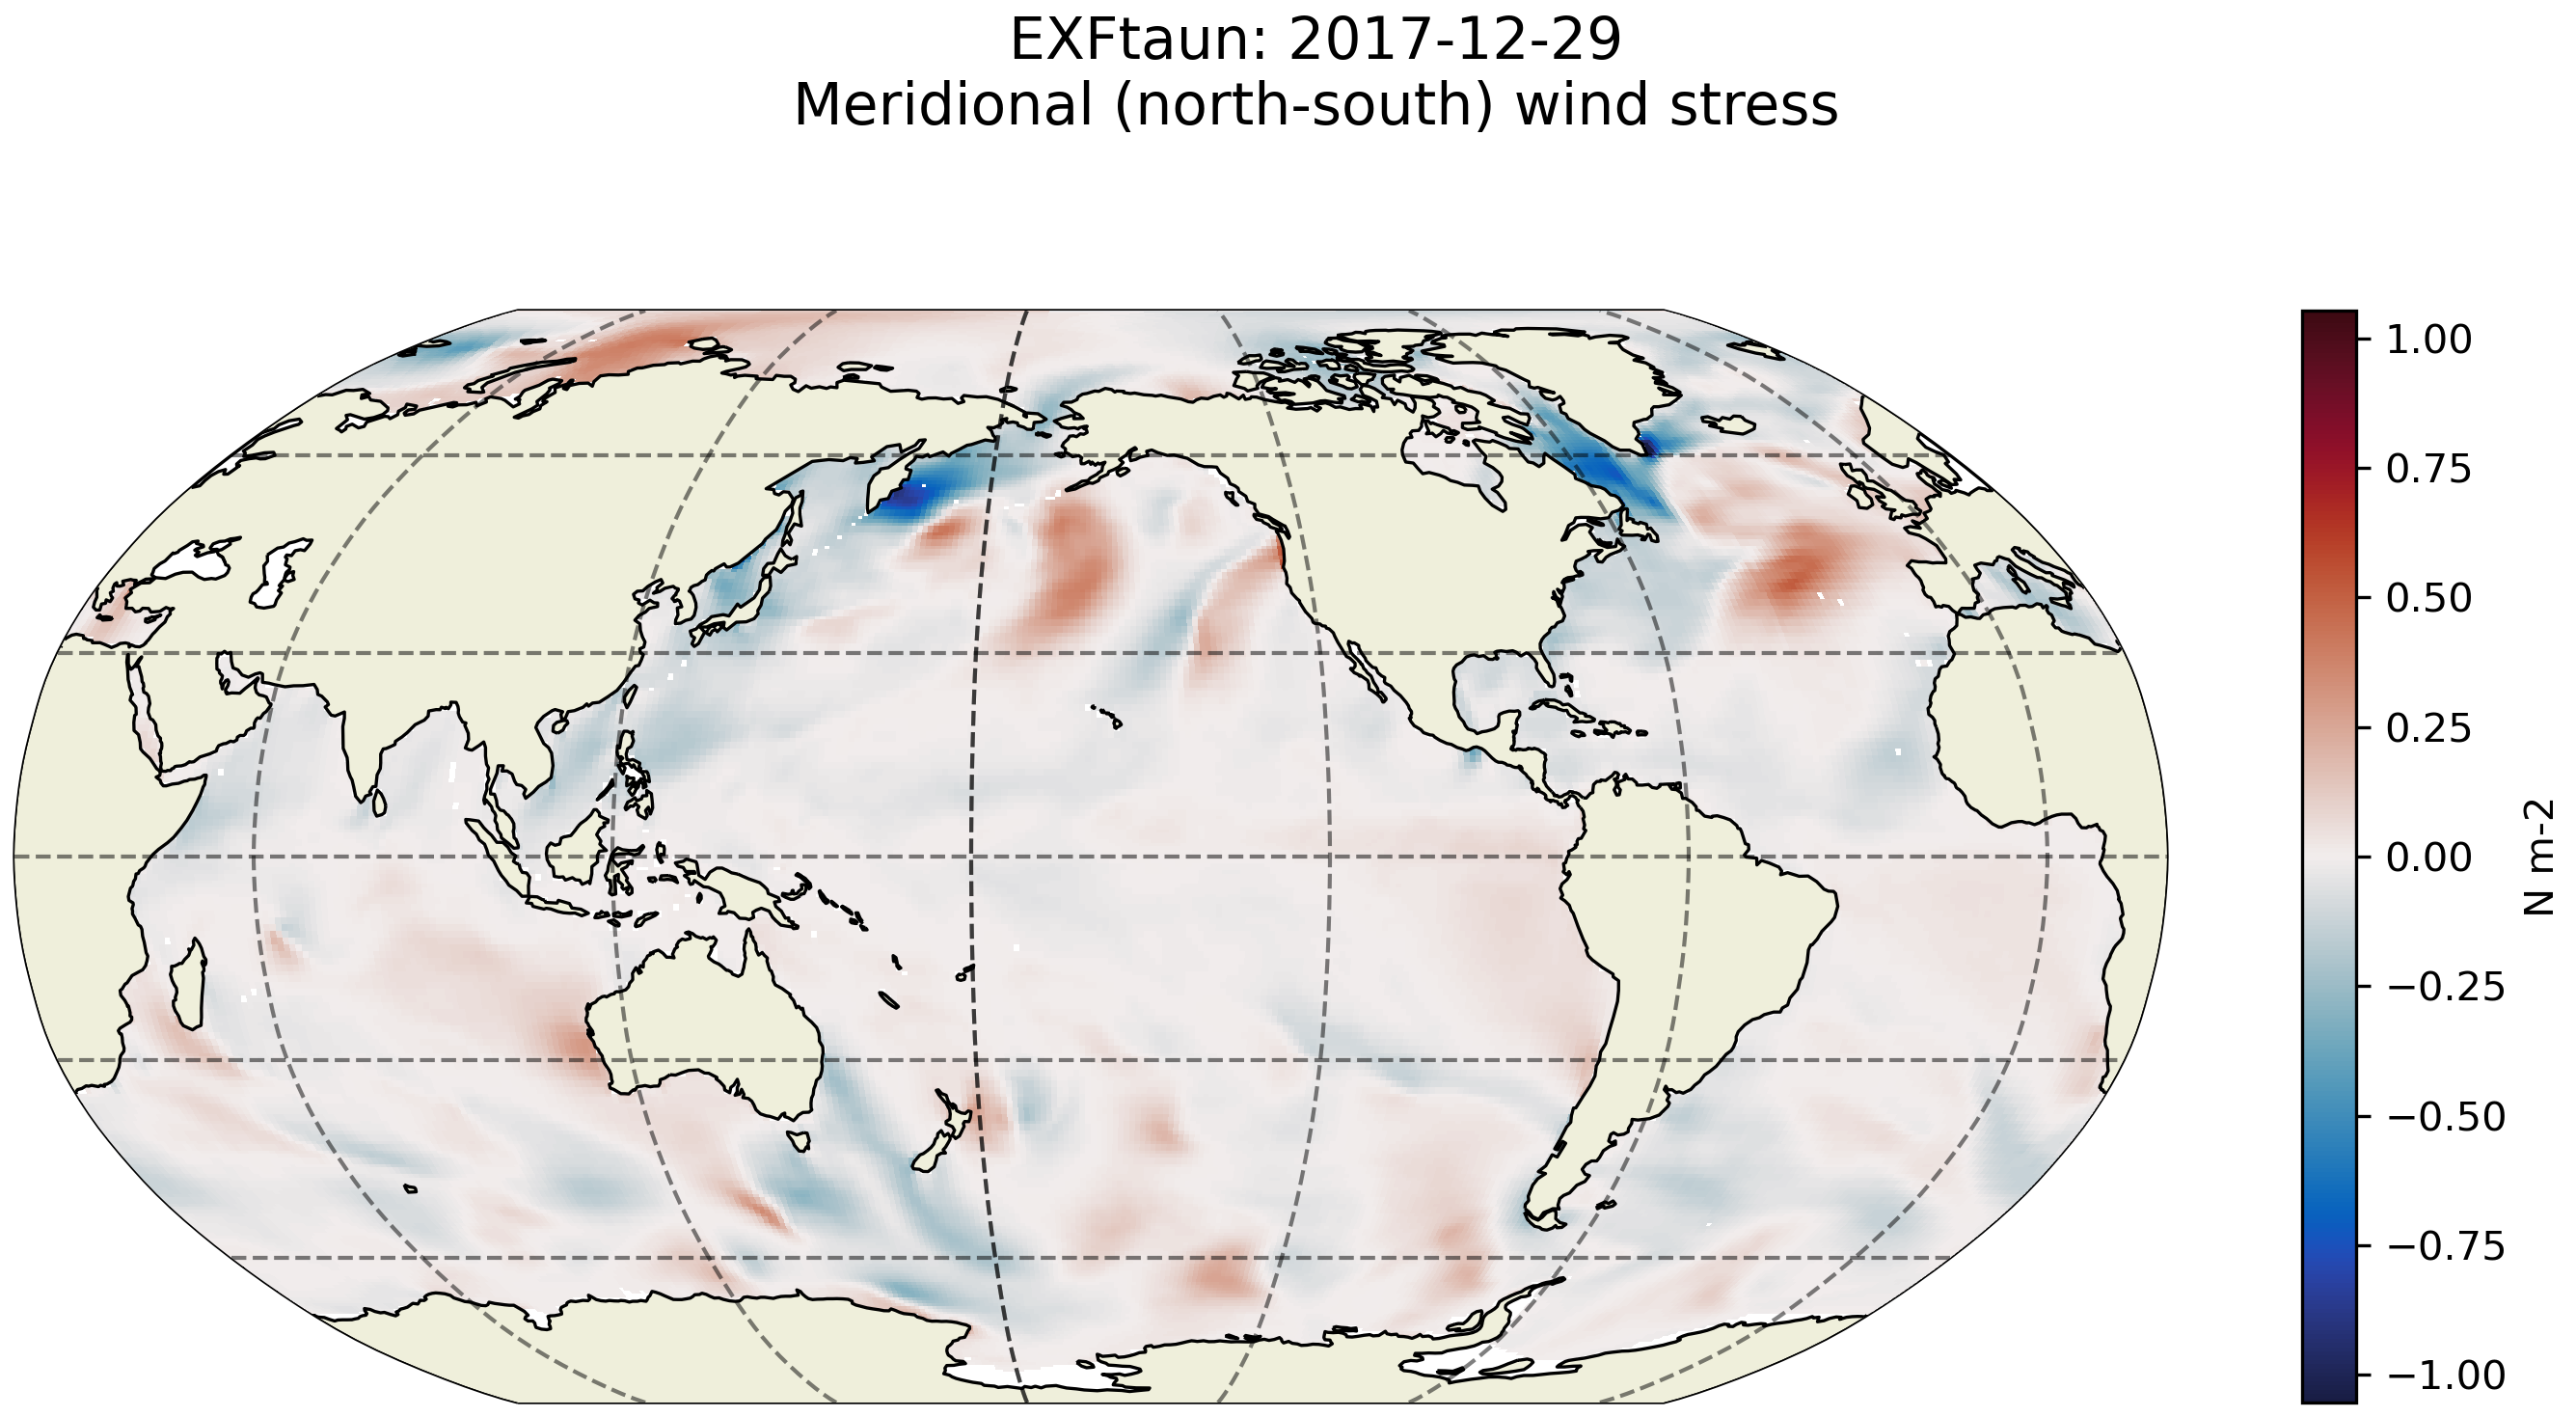
\includegraphics[width=\textwidth]{../images/plots/latlon_plots/Ocean_and_Sea-Ice_Surface_Stress/EXFtaun.png}
\caption{Dataset: OCEAN\_AND\_ICE\_SURFACE\_STRESS Variable: EXFtaun}
\label{tab:table-OCEAN_AND_ICE_SURFACE_STRESS_EXFtaun-Plot}
\end{figure}
\pagebreak
\subsubsection{Latlon Variable oceTAUE}
\begin{longtable}{|p{0.06\textwidth}|p{0.41\textwidth}|p{0.39\textwidth}|p{0.06\textwidth}|}
\caption{CDL description of OCEAN\_AND\_ICE\_SURFACE\_STRESS's oceTAUE variable}
\label{tab:table-OCEAN_AND_ICE_SURFACE_STRESS_oceTAUE} \\ 
\hline \endhead \hline \endfoot
\rowcolor{lightgray} \textbf{Storage Type} & \textbf{Variable Name} & \textbf{Description} & \textbf{Unit} \\ \hline
float32 & oceTAUE & Zonal (east-west) ocean surface stress & N m-2 \\ \hline
\rowcolor{lightgray}  \multicolumn{4}{|p{1.00\textwidth}|}{\textbf{CDL Description}} \\ \hline
\multicolumn{4}{|p{1.00\textwidth}|}{\makecell{\parbox{1\textwidth}{float32 oceTAUE(time, latitude, longitude)\\
\hspace*{0.5cm}oceTAUE: \_FillValue = 9.96921e+36\\
\hspace*{0.5cm}oceTAUE: coverage\_content\_type = modelResult\\
\hspace*{0.5cm}oceTAUE: direction =  >0 increases eastward velocity (EVEL)\\
\hspace*{0.5cm}oceTAUE: long\_name = Zonal (east: west) ocean surface stress\\
\hspace*{0.5cm}oceTAUE: standard\_name = surface\_downward\_eastward\_stress\\
\hspace*{0.5cm}oceTAUE: units = N m: 2\\
\hspace*{0.5cm}oceTAUE: coordinates = time\\
\hspace*{0.5cm}oceTAUE: valid\_min = : 2.058817148208618\\
\hspace*{0.5cm}oceTAUE: valid\_max = 2.000103712081909}}} \\ \hline
\rowcolor{lightgray} \multicolumn{4}{|p{1.00\textwidth}|}{\textbf{Comments}} \\ \hline
\multicolumn{4}{|p{1\textwidth}|}{Zonal (east-west) component of ocean surface stress due to wind and sea-ice. Note: oceTAUE is calculated by interpolating the model's x and y components of ocean surface stress (oceTAUX and oceTAUY) to tracer cell centers and then finding the zonal component of the interpolated vectors.} \\ \hline
\end{longtable}

\begin{figure}[H]
\centering
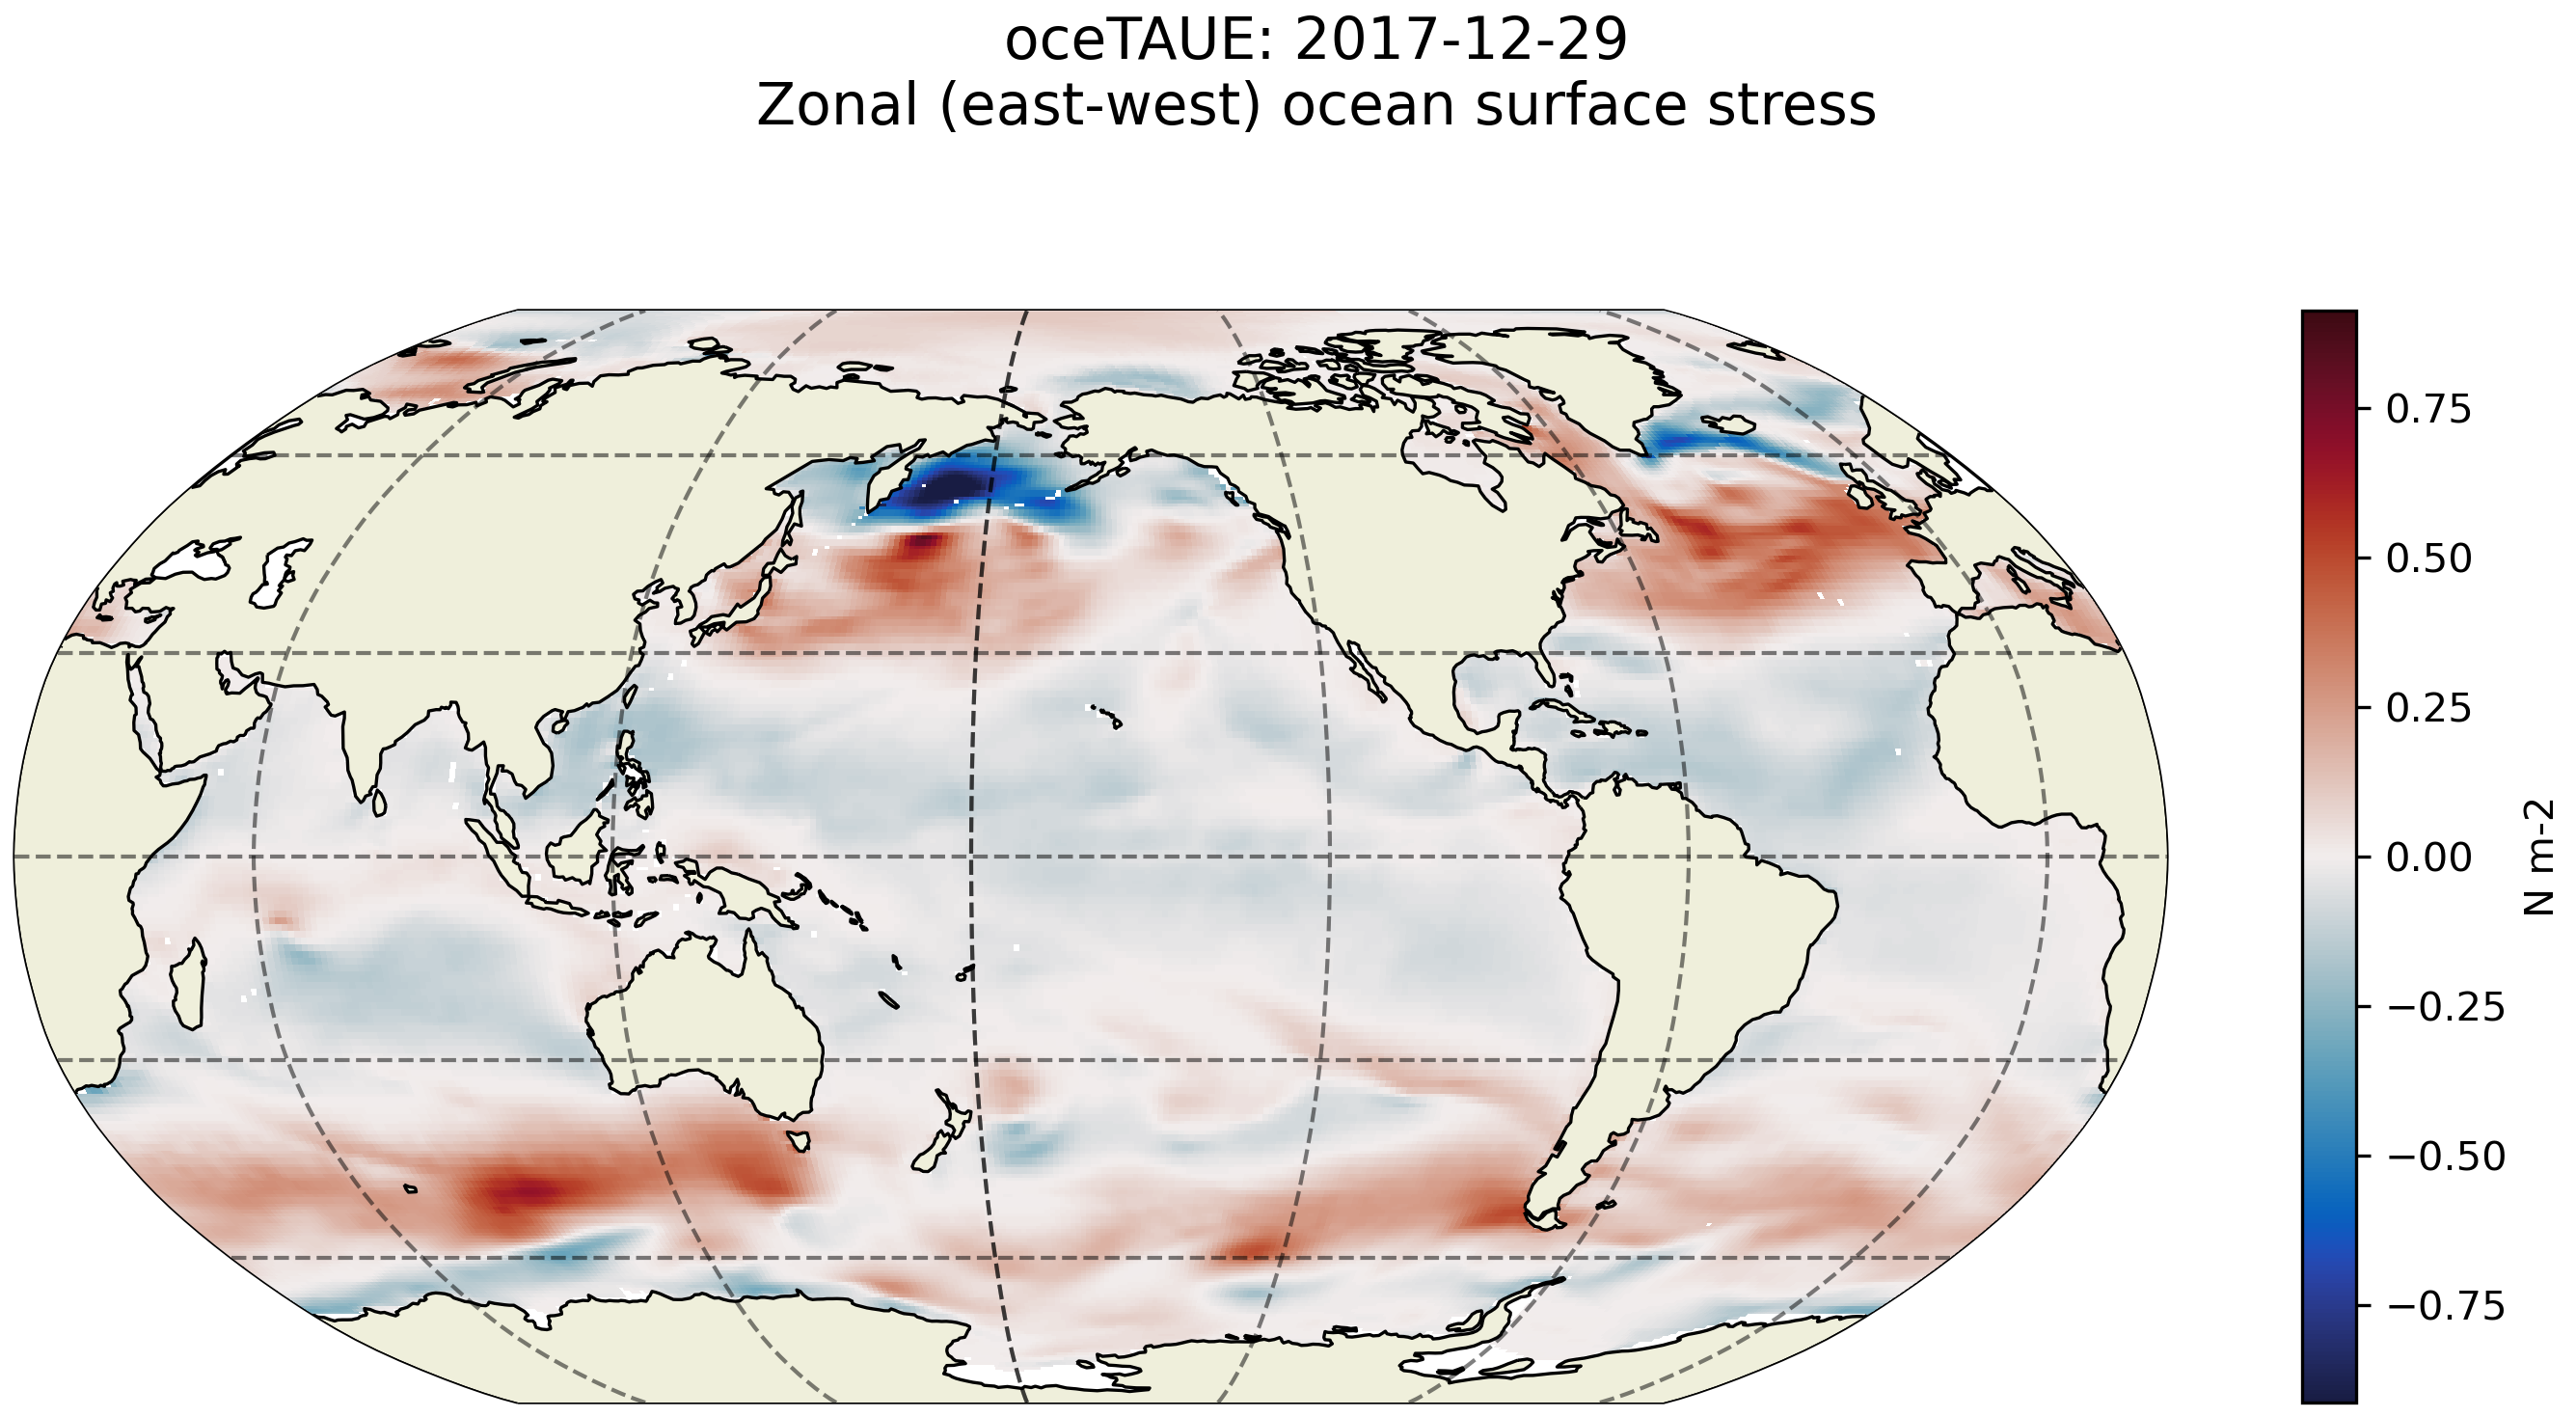
\includegraphics[width=\textwidth]{../images/plots/latlon_plots/Ocean_and_Sea-Ice_Surface_Stress/oceTAUE.png}
\caption{Dataset: OCEAN\_AND\_ICE\_SURFACE\_STRESS Variable: oceTAUE}
\label{tab:table-OCEAN_AND_ICE_SURFACE_STRESS_oceTAUE-Plot}
\end{figure}
\pagebreak
\subsubsection{Latlon Variable oceTAUN}
\begin{longtable}{|p{0.06\textwidth}|p{0.41\textwidth}|p{0.39\textwidth}|p{0.06\textwidth}|}
\caption{CDL description of OCEAN\_AND\_ICE\_SURFACE\_STRESS's oceTAUN variable}
\label{tab:table-OCEAN_AND_ICE_SURFACE_STRESS_oceTAUN} \\ 
\hline \endhead \hline \endfoot
\rowcolor{lightgray} \textbf{Storage Type} & \textbf{Variable Name} & \textbf{Description} & \textbf{Unit} \\ \hline
float32 & oceTAUN & Meridional (north-south) ocean surface stress & N m-2 \\ \hline
\rowcolor{lightgray}  \multicolumn{4}{|p{1.00\textwidth}|}{\textbf{CDL Description}} \\ \hline
\multicolumn{4}{|p{1.00\textwidth}|}{\makecell{\parbox{1\textwidth}{float32 oceTAUN(time, latitude, longitude)\\
\hspace*{0.5cm}oceTAUN: \_FillValue = 9.96921e+36\\
\hspace*{0.5cm}oceTAUN: coverage\_content\_type = modelResult\\
\hspace*{0.5cm}oceTAUN: direction =  >0 increases northward velocity (NVEL)\\
\hspace*{0.5cm}oceTAUN: long\_name = Meridional (north: south) ocean surface stress\\
\hspace*{0.5cm}oceTAUN: standard\_name = surface\_downward\_northward\_stress\\
\hspace*{0.5cm}oceTAUN: units = N m: 2\\
\hspace*{0.5cm}oceTAUN: coordinates = time\\
\hspace*{0.5cm}oceTAUN: valid\_min = : 2.4036266803741455\\
\hspace*{0.5cm}oceTAUN: valid\_max = 2.019313097000122}}} \\ \hline
\rowcolor{lightgray} \multicolumn{4}{|p{1.00\textwidth}|}{\textbf{Comments}} \\ \hline
\multicolumn{4}{|p{1\textwidth}|}{Meridional (north-south) component of ocean surface stress due to wind and sea-ice. Note: oceTAUN is calculated by interpolating the model's x and y components of ocean surface stress (oceTAUX and oceTAUY) to tracer cell centers and then finding the meridional component of the interpolated vectors.} \\ \hline
\end{longtable}

\begin{figure}[H]
\centering
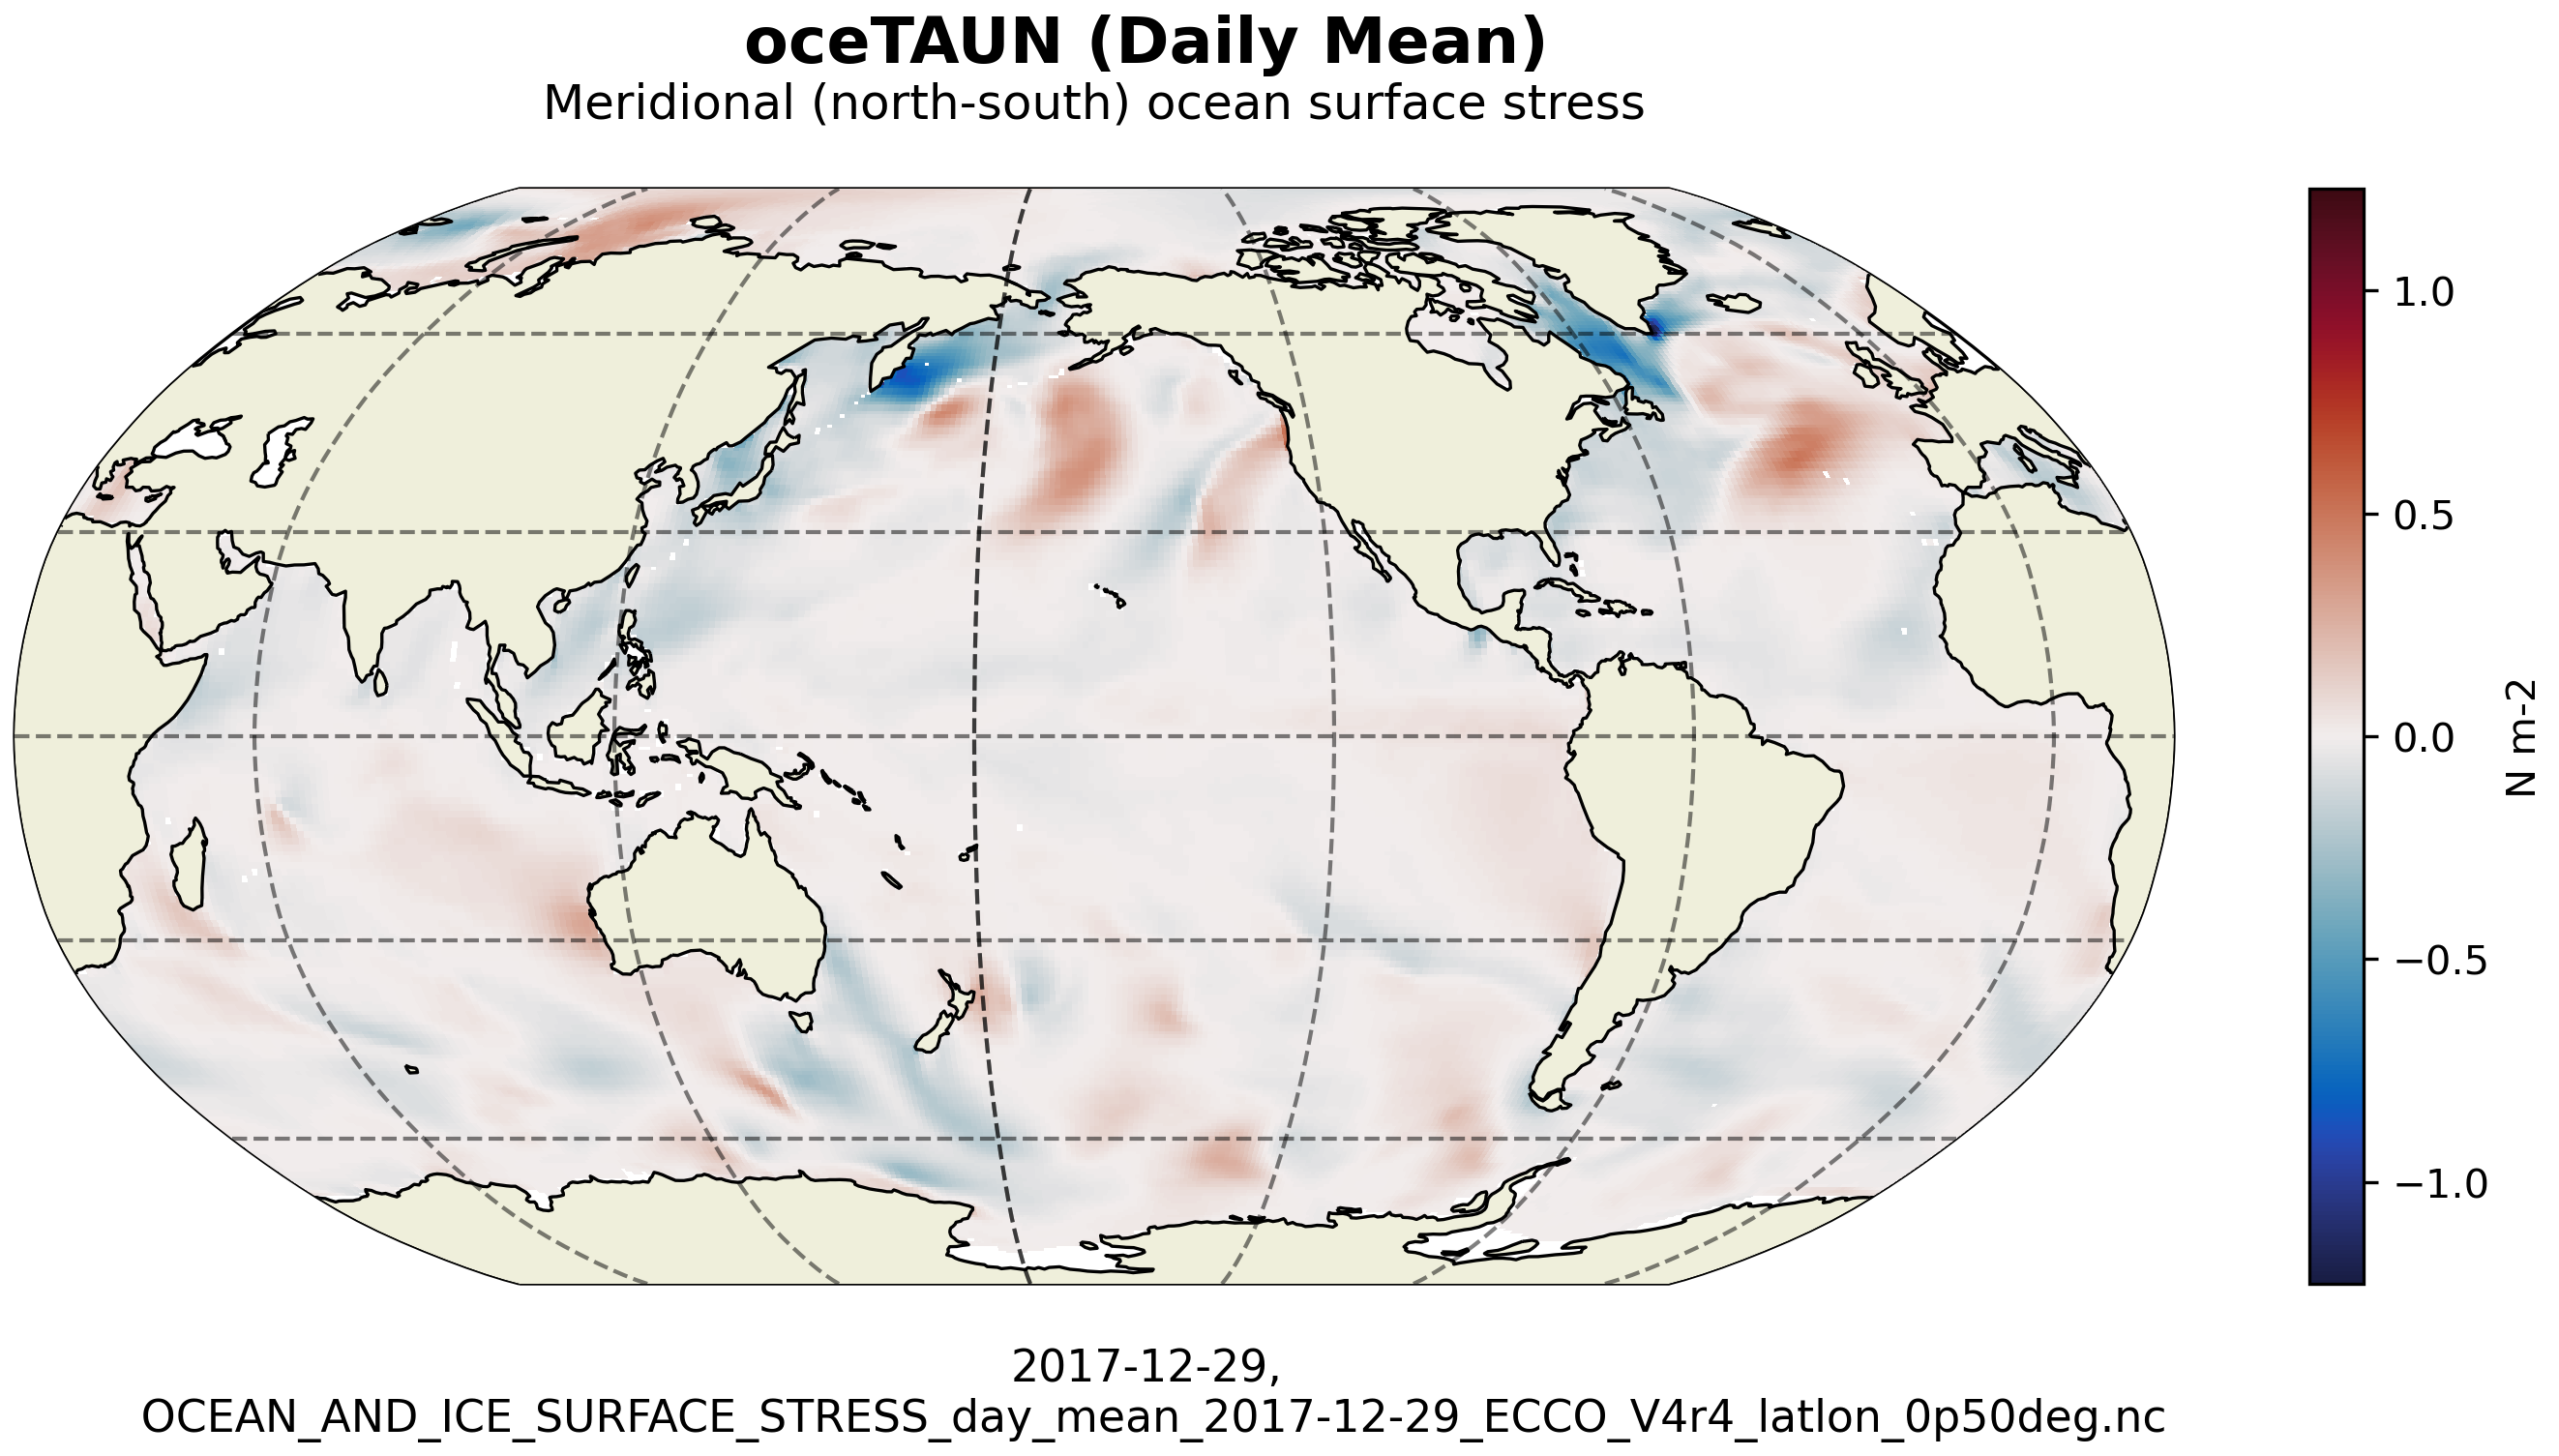
\includegraphics[width=\textwidth]{../images/plots/latlon_plots/Ocean_and_Sea-Ice_Surface_Stress/oceTAUN.png}
\caption{Dataset: OCEAN\_AND\_ICE\_SURFACE\_STRESS Variable: oceTAUN}
\label{tab:table-OCEAN_AND_ICE_SURFACE_STRESS_oceTAUN-Plot}
\end{figure}
\pagebreak
\subsection{Latlon NetCDF OCEAN\_BOLUS\_VELOCITY}
\newp
\begin{longtable}{|p{0.1\textwidth}|p{0.5\textwidth}|}
\caption{Variables in the dataset OCEAN\_BOLUS\_VELOCITY}
\label{tab:table-OCEAN_BOLUS_VELOCITY-fields} \\ 
\hline \endhead \hline \endfoot
\rowcolor{lightgray} \textbf{Dataset:} & \textbf{OCEAN\_BOLUS\_VELOCITY} \\ \hline
Field: &EVELSTAR \\ \hline
Field: &NVELSTAR \\ \hline
Field: &WVELSTAR \\ \hline
\end{longtable}

\pagebreak
\subsubsection{Latlon Variable EVELSTAR}
\begin{longtable}{|p{0.06\textwidth}|p{0.41\textwidth}|p{0.39\textwidth}|p{0.06\textwidth}|}
\caption{CDL description of OCEAN\_BOLUS\_VELOCITY's EVELSTAR variable}
\label{tab:table-OCEAN_BOLUS_VELOCITY_EVELSTAR} \\ 
\hline \endhead \hline \endfoot
\rowcolor{lightgray} \textbf{Storage Type} & \textbf{Variable Name} & \textbf{Description} & \textbf{Unit} \\ \hline
float32 & EVELSTAR & Gent-McWilliams zonal (east-west) bolus velocity & m s-1 \\ \hline
\rowcolor{lightgray}  \multicolumn{4}{|p{1.00\textwidth}|}{\textbf{CDL Description}} \\ \hline
\multicolumn{4}{|p{1.00\textwidth}|}{\makecell{\parbox{1\textwidth}{float32 EVELSTAR(time, Z, latitude, longitude)\\
\hspace*{0.5cm}EVELSTAR: \_FillValue = 9.96921e+36\\
\hspace*{0.5cm}EVELSTAR: coverage\_content\_type = modelResult\\
\hspace*{0.5cm}EVELSTAR: long\_name = Gent: McWilliams zonal (east: west) bolus velocity\\
\hspace*{0.5cm}EVELSTAR: standard\_name = eastward\_sea\_water\_velocity\_due\_to\_parameterized\_mesoscale\_eddies\\
\hspace*{0.5cm}EVELSTAR: units = m s: 1\\
\hspace*{0.5cm}EVELSTAR: coordinates = time Z\\
\hspace*{0.5cm}EVELSTAR: valid\_min = : 0.5832233428955078\\
\hspace*{0.5cm}EVELSTAR: valid\_max = 0.7810457944869995}}} \\ \hline
\rowcolor{lightgray} \multicolumn{4}{|p{1.00\textwidth}|}{\textbf{Comments}} \\ \hline
\multicolumn{4}{|p{1\textwidth}|}{Zonal (east-west) component of the Gent-McWilliams bolus ocean velocity. Note: EVELSTAR is calculated by interpolating the model's x and y components of GM bolus ocean velocity (UVELSTAR and VVELSTAR) to tracer cell centers and then finding the zonal components of the interpolated vectors. One should take care when interpreting bolus velocities interpolated from the ECCO native model grid because interpolating from the model grid to the lat-lon grid introduces errors. Some closed buget calculations require bolus velocity terms on the native model grid.} \\ \hline
\end{longtable}

\begin{figure}[H]
\centering
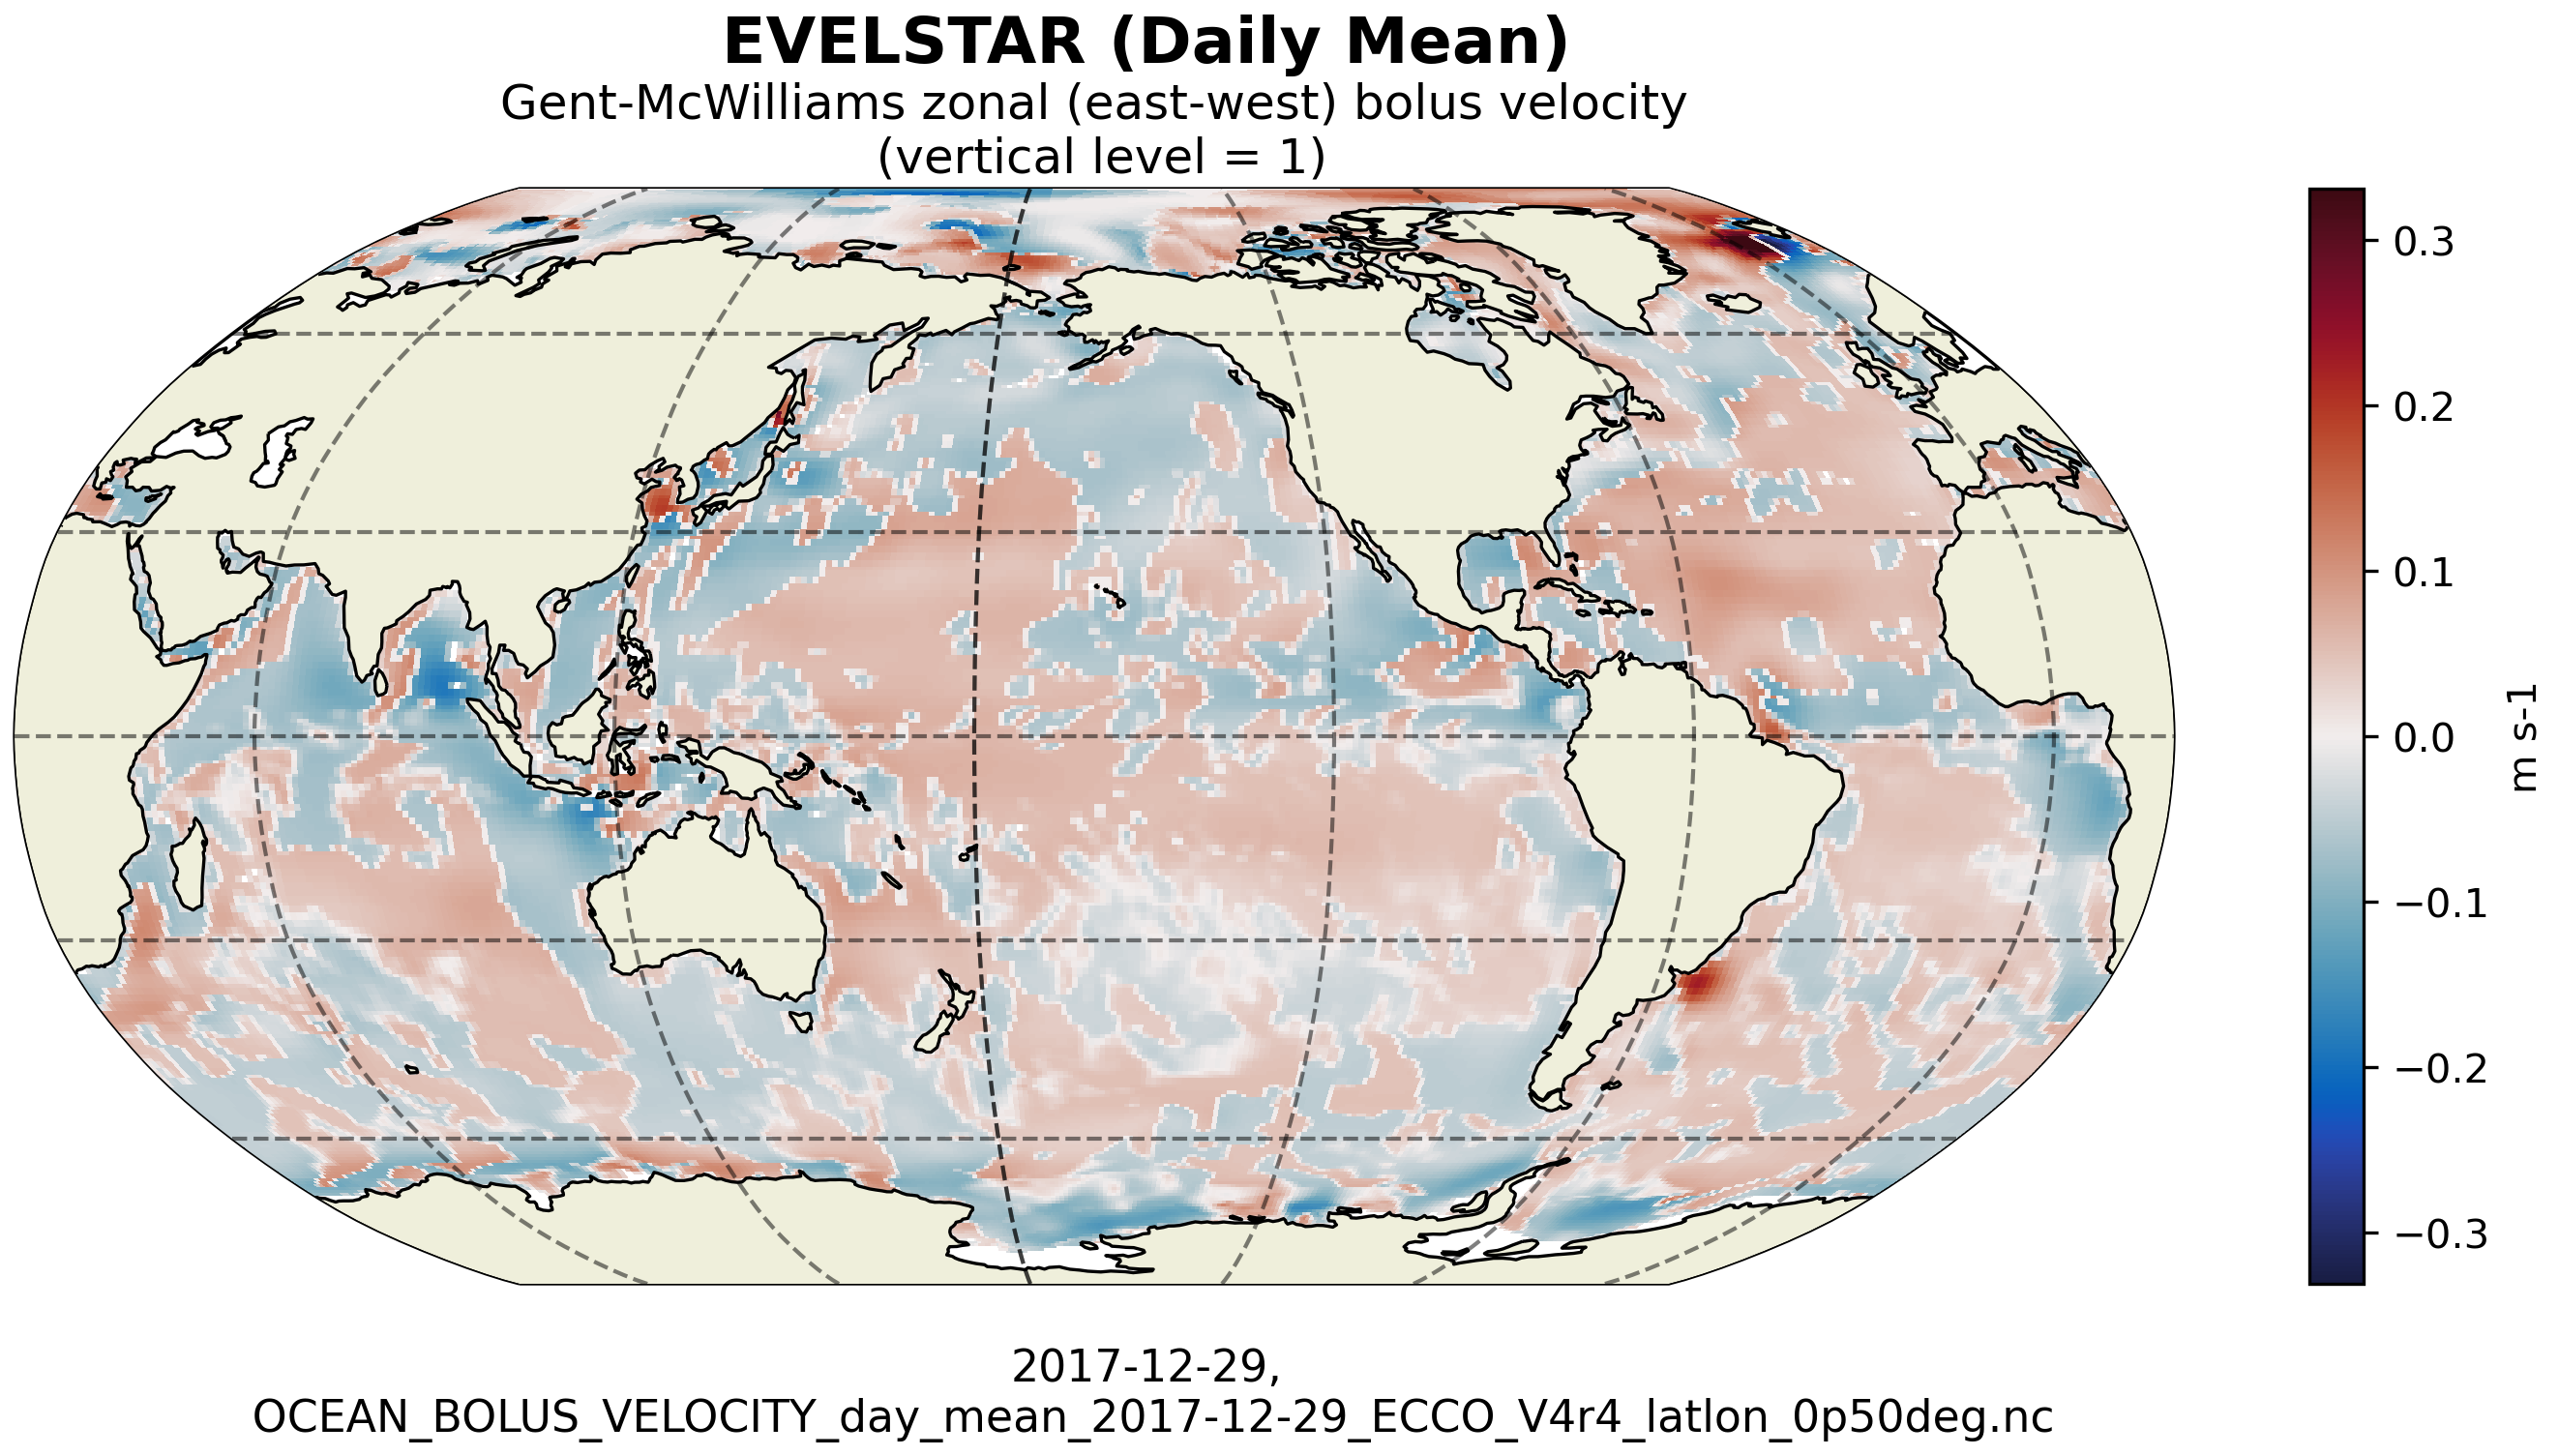
\includegraphics[width=\textwidth]{../images/plots/latlon_plots/Gent-McWilliams_Ocean_Bolus_Velocity/EVELSTAR.png}
\caption{Dataset: OCEAN\_BOLUS\_VELOCITY Variable: EVELSTAR}
\label{tab:table-OCEAN_BOLUS_VELOCITY_EVELSTAR-Plot}
\end{figure}
\pagebreak
\subsubsection{Latlon Variable NVELSTAR}
\begin{longtable}{|p{0.06\textwidth}|p{0.41\textwidth}|p{0.39\textwidth}|p{0.06\textwidth}|}
\caption{CDL description of OCEAN\_BOLUS\_VELOCITY's NVELSTAR variable}
\label{tab:table-OCEAN_BOLUS_VELOCITY_NVELSTAR} \\ 
\hline \endhead \hline \endfoot
\rowcolor{lightgray} \textbf{Storage Type} & \textbf{Variable Name} & \textbf{Description} & \textbf{Unit} \\ \hline
float32 & NVELSTAR & Gent-McWilliams meridional (north-south) bolus velocity & m s-1 \\ \hline
\rowcolor{lightgray}  \multicolumn{4}{|p{1.00\textwidth}|}{\textbf{CDL Description}} \\ \hline
\multicolumn{4}{|p{1.00\textwidth}|}{\makecell{\parbox{1\textwidth}{float32 NVELSTAR(time, Z, latitude, longitude)\\
\hspace*{0.5cm}NVELSTAR: \_FillValue = 9.96921e+36\\
\hspace*{0.5cm}NVELSTAR: coverage\_content\_type = modelResult\\
\hspace*{0.5cm}NVELSTAR: long\_name = Gent: McWilliams meridional (north: south) bolus velocity\\
\hspace*{0.5cm}NVELSTAR: standard\_name = northward\_sea\_water\_velocity\_due\_to\_parameterized\_mesoscale\_eddies\\
\hspace*{0.5cm}NVELSTAR: units = m s: 1\\
\hspace*{0.5cm}NVELSTAR: coordinates = time Z\\
\hspace*{0.5cm}NVELSTAR: valid\_min = : 0.6472858190536499\\
\hspace*{0.5cm}NVELSTAR: valid\_max = 0.6751338243484497}}} \\ \hline
\rowcolor{lightgray} \multicolumn{4}{|p{1.00\textwidth}|}{\textbf{Comments}} \\ \hline
\multicolumn{4}{|p{1\textwidth}|}{Meridional (north-south) component of the Gent-McWilliams bolus ocean velocity. Note: NVELSTAR is calculated by interpolating the model's x and y components of GM bolus ocean velocity (UVELSTAR and VVELSTAR) to tracer cell centers and then finding the meridional components of the interpolated vectors.  One should take care when interpreting bolus velocities interpolated from the ECCO native model grid because interpolating from the model grid to the lat-lon grid introduces errors. Some closed buget calculations require bolus velocity terms on the native model grid} \\ \hline
\end{longtable}

\begin{figure}[H]
\centering
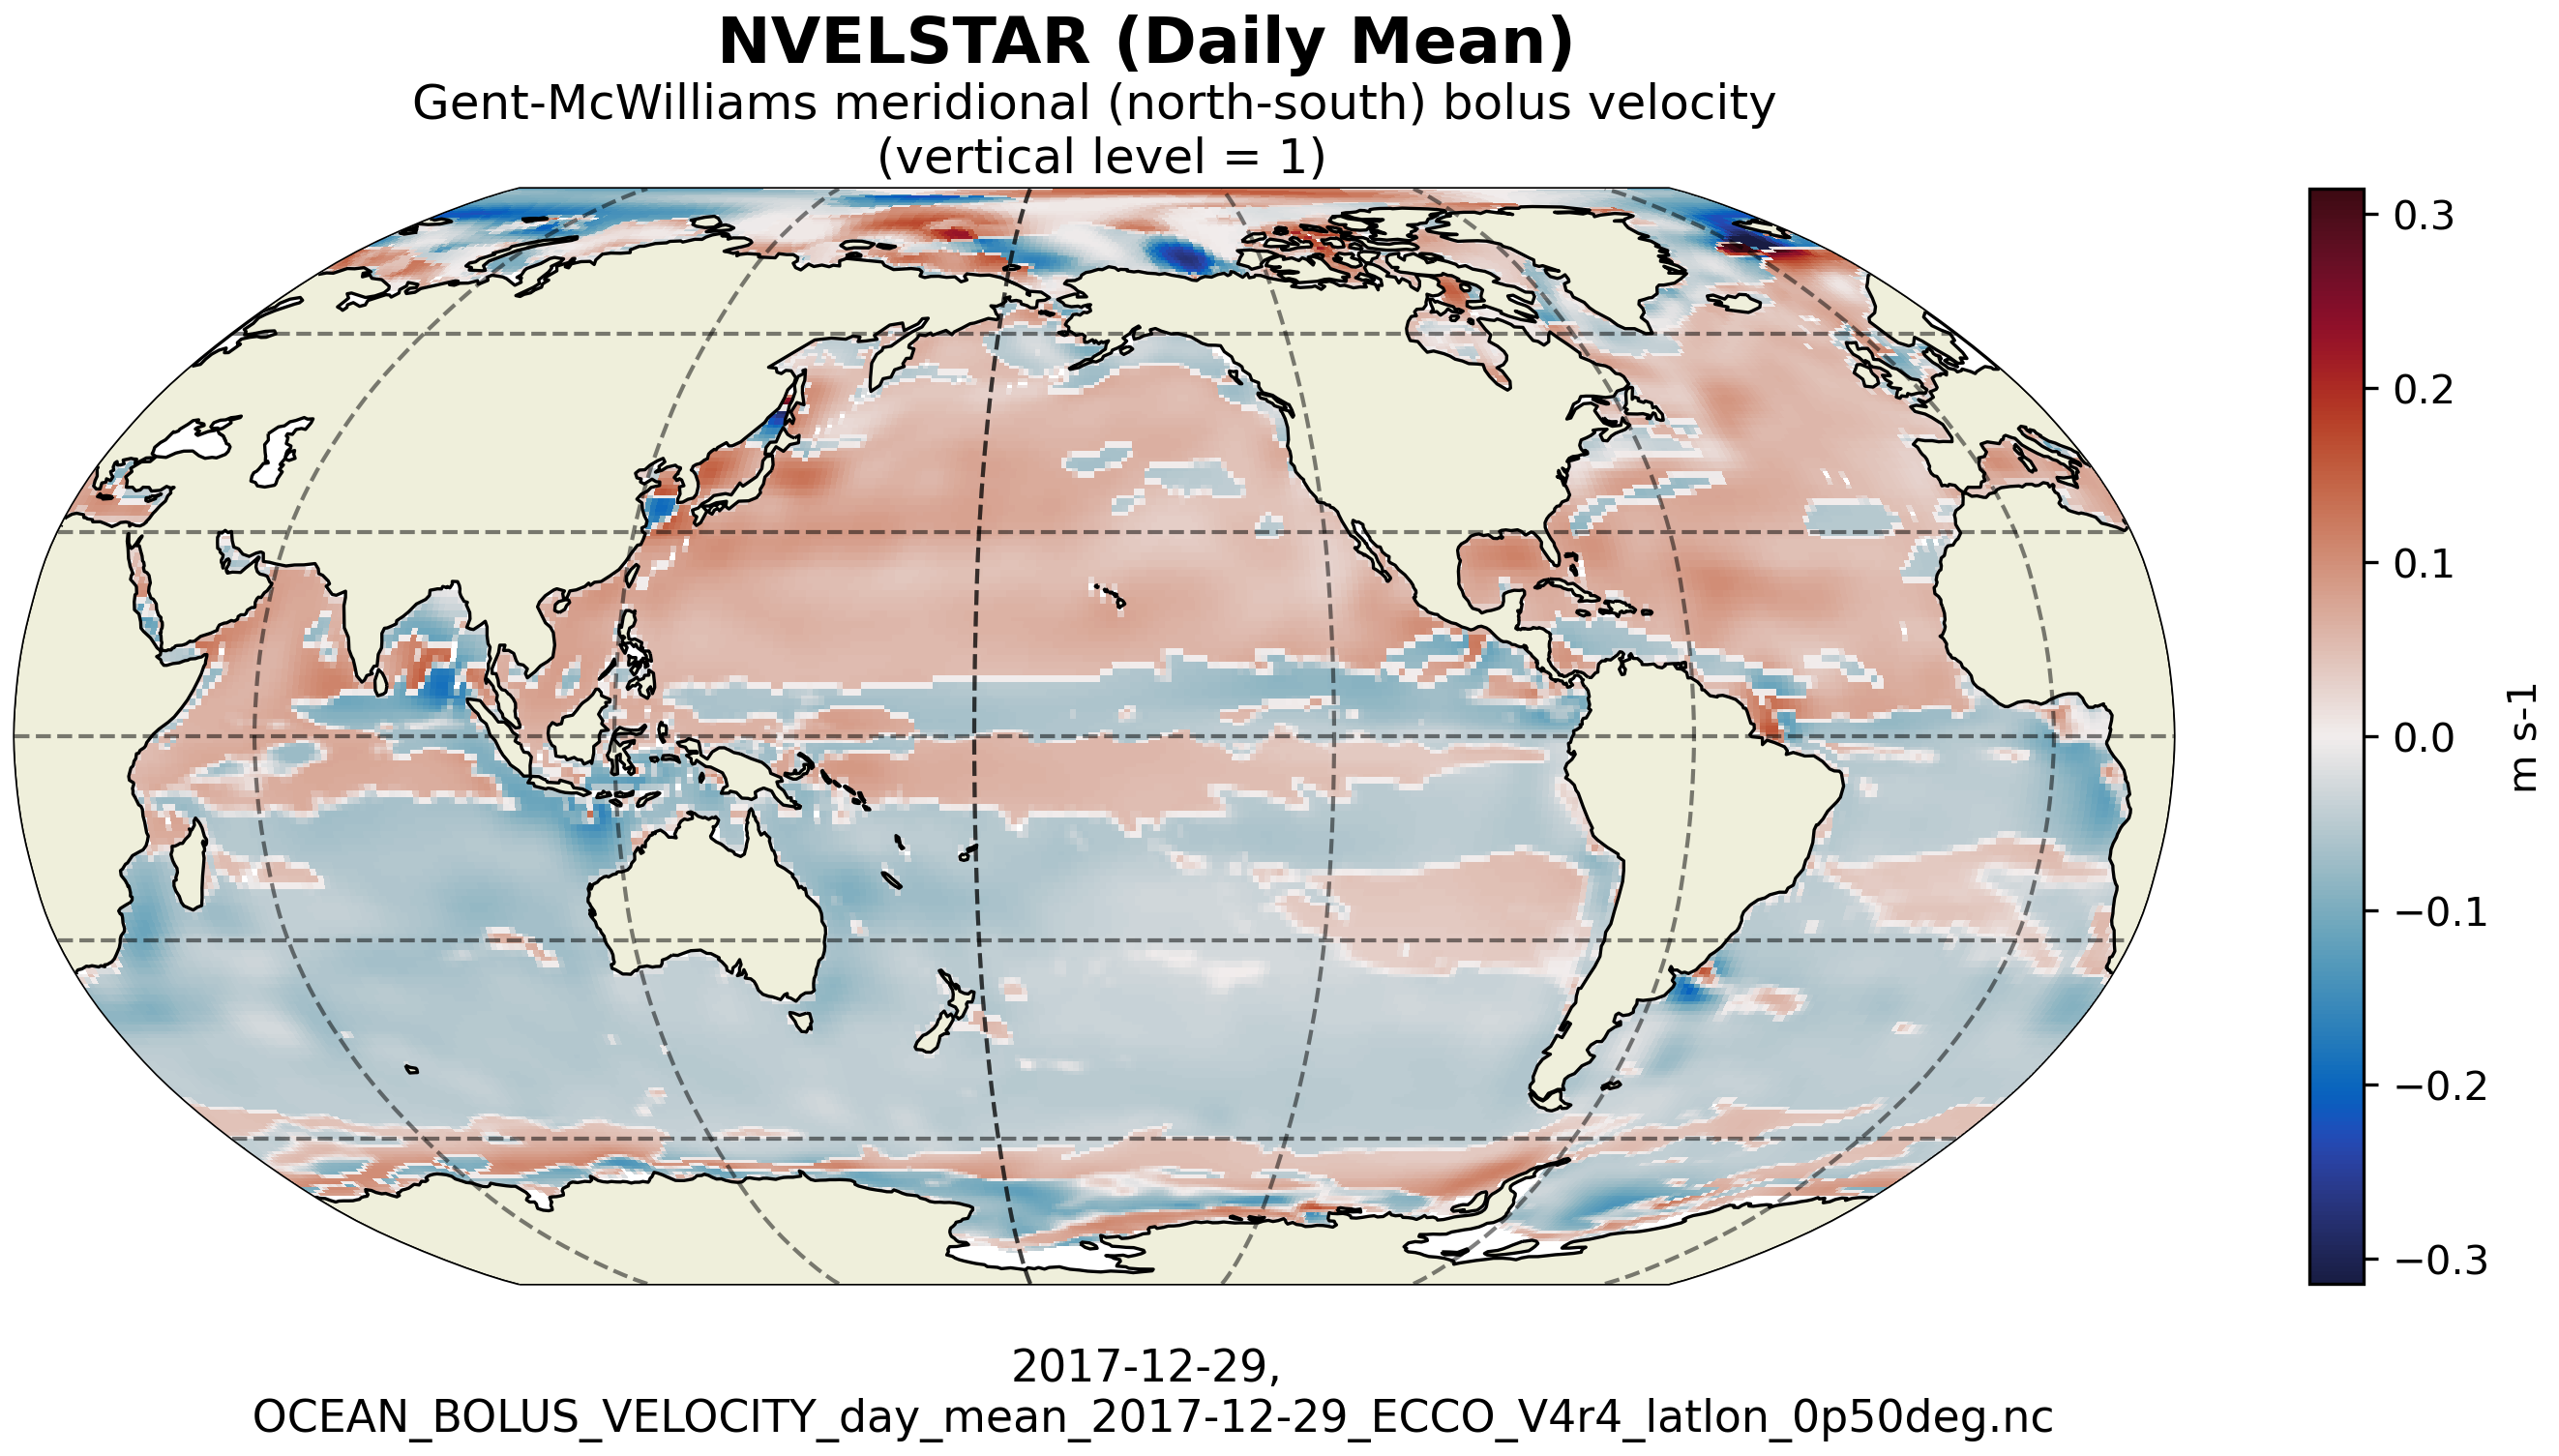
\includegraphics[width=\textwidth]{../images/plots/latlon_plots/Gent-McWilliams_Ocean_Bolus_Velocity/NVELSTAR.png}
\caption{Dataset: OCEAN\_BOLUS\_VELOCITY Variable: NVELSTAR}
\label{tab:table-OCEAN_BOLUS_VELOCITY_NVELSTAR-Plot}
\end{figure}
\pagebreak
\subsubsection{Latlon Variable WVELSTAR}
\begin{longtable}{|p{0.06\textwidth}|p{0.41\textwidth}|p{0.39\textwidth}|p{0.06\textwidth}|}
\caption{CDL description of OCEAN\_BOLUS\_VELOCITY's WVELSTAR variable}
\label{tab:table-OCEAN_BOLUS_VELOCITY_WVELSTAR} \\ 
\hline \endhead \hline \endfoot
\rowcolor{lightgray} \textbf{Storage Type} & \textbf{Variable Name} & \textbf{Description} & \textbf{Unit} \\ \hline
float32 & WVELSTAR & Gent-McWilliams vertical bolus velocity & m s-1 \\ \hline
\rowcolor{lightgray}  \multicolumn{4}{|p{1.00\textwidth}|}{\textbf{CDL Description}} \\ \hline
\multicolumn{4}{|p{1.00\textwidth}|}{\makecell{\parbox{1\textwidth}{float32 WVELSTAR(time, Z, latitude, longitude)\\
\hspace*{0.5cm}WVELSTAR: \_FillValue = 9.96921e+36\\
\hspace*{0.5cm}WVELSTAR: coverage\_content\_type = modelResult\\
\hspace*{0.5cm}WVELSTAR: direction = >0 decreases volume\\
\hspace*{0.5cm}WVELSTAR: long\_name = Gent: McWilliams vertical bolus velocity\\
\hspace*{0.5cm}WVELSTAR: standard\_name = upward\_sea\_water\_velocity\_due\_to\_parameterized\_mesoscale\_eddies\\
\hspace*{0.5cm}WVELSTAR: units = m s: 1\\
\hspace*{0.5cm}WVELSTAR: coordinates = time Z\\
\hspace*{0.5cm}WVELSTAR: valid\_min = : 0.00037936007720418274\\
\hspace*{0.5cm}WVELSTAR: valid\_max = 0.0004019034677185118}}} \\ \hline
\rowcolor{lightgray} \multicolumn{4}{|p{1.00\textwidth}|}{\textbf{Comments}} \\ \hline
\multicolumn{4}{|p{1\textwidth}|}{Vertical component of the Gent-McWilliams bolus ocean velocity. Note: in the Arakawa-C grid used in ECCO V4r4, vertical velocities are staggered relative to the tracer cell centers with values at the TOP and BOTTOM faces of each grid cell.} \\ \hline
\end{longtable}

\begin{figure}[H]
\centering
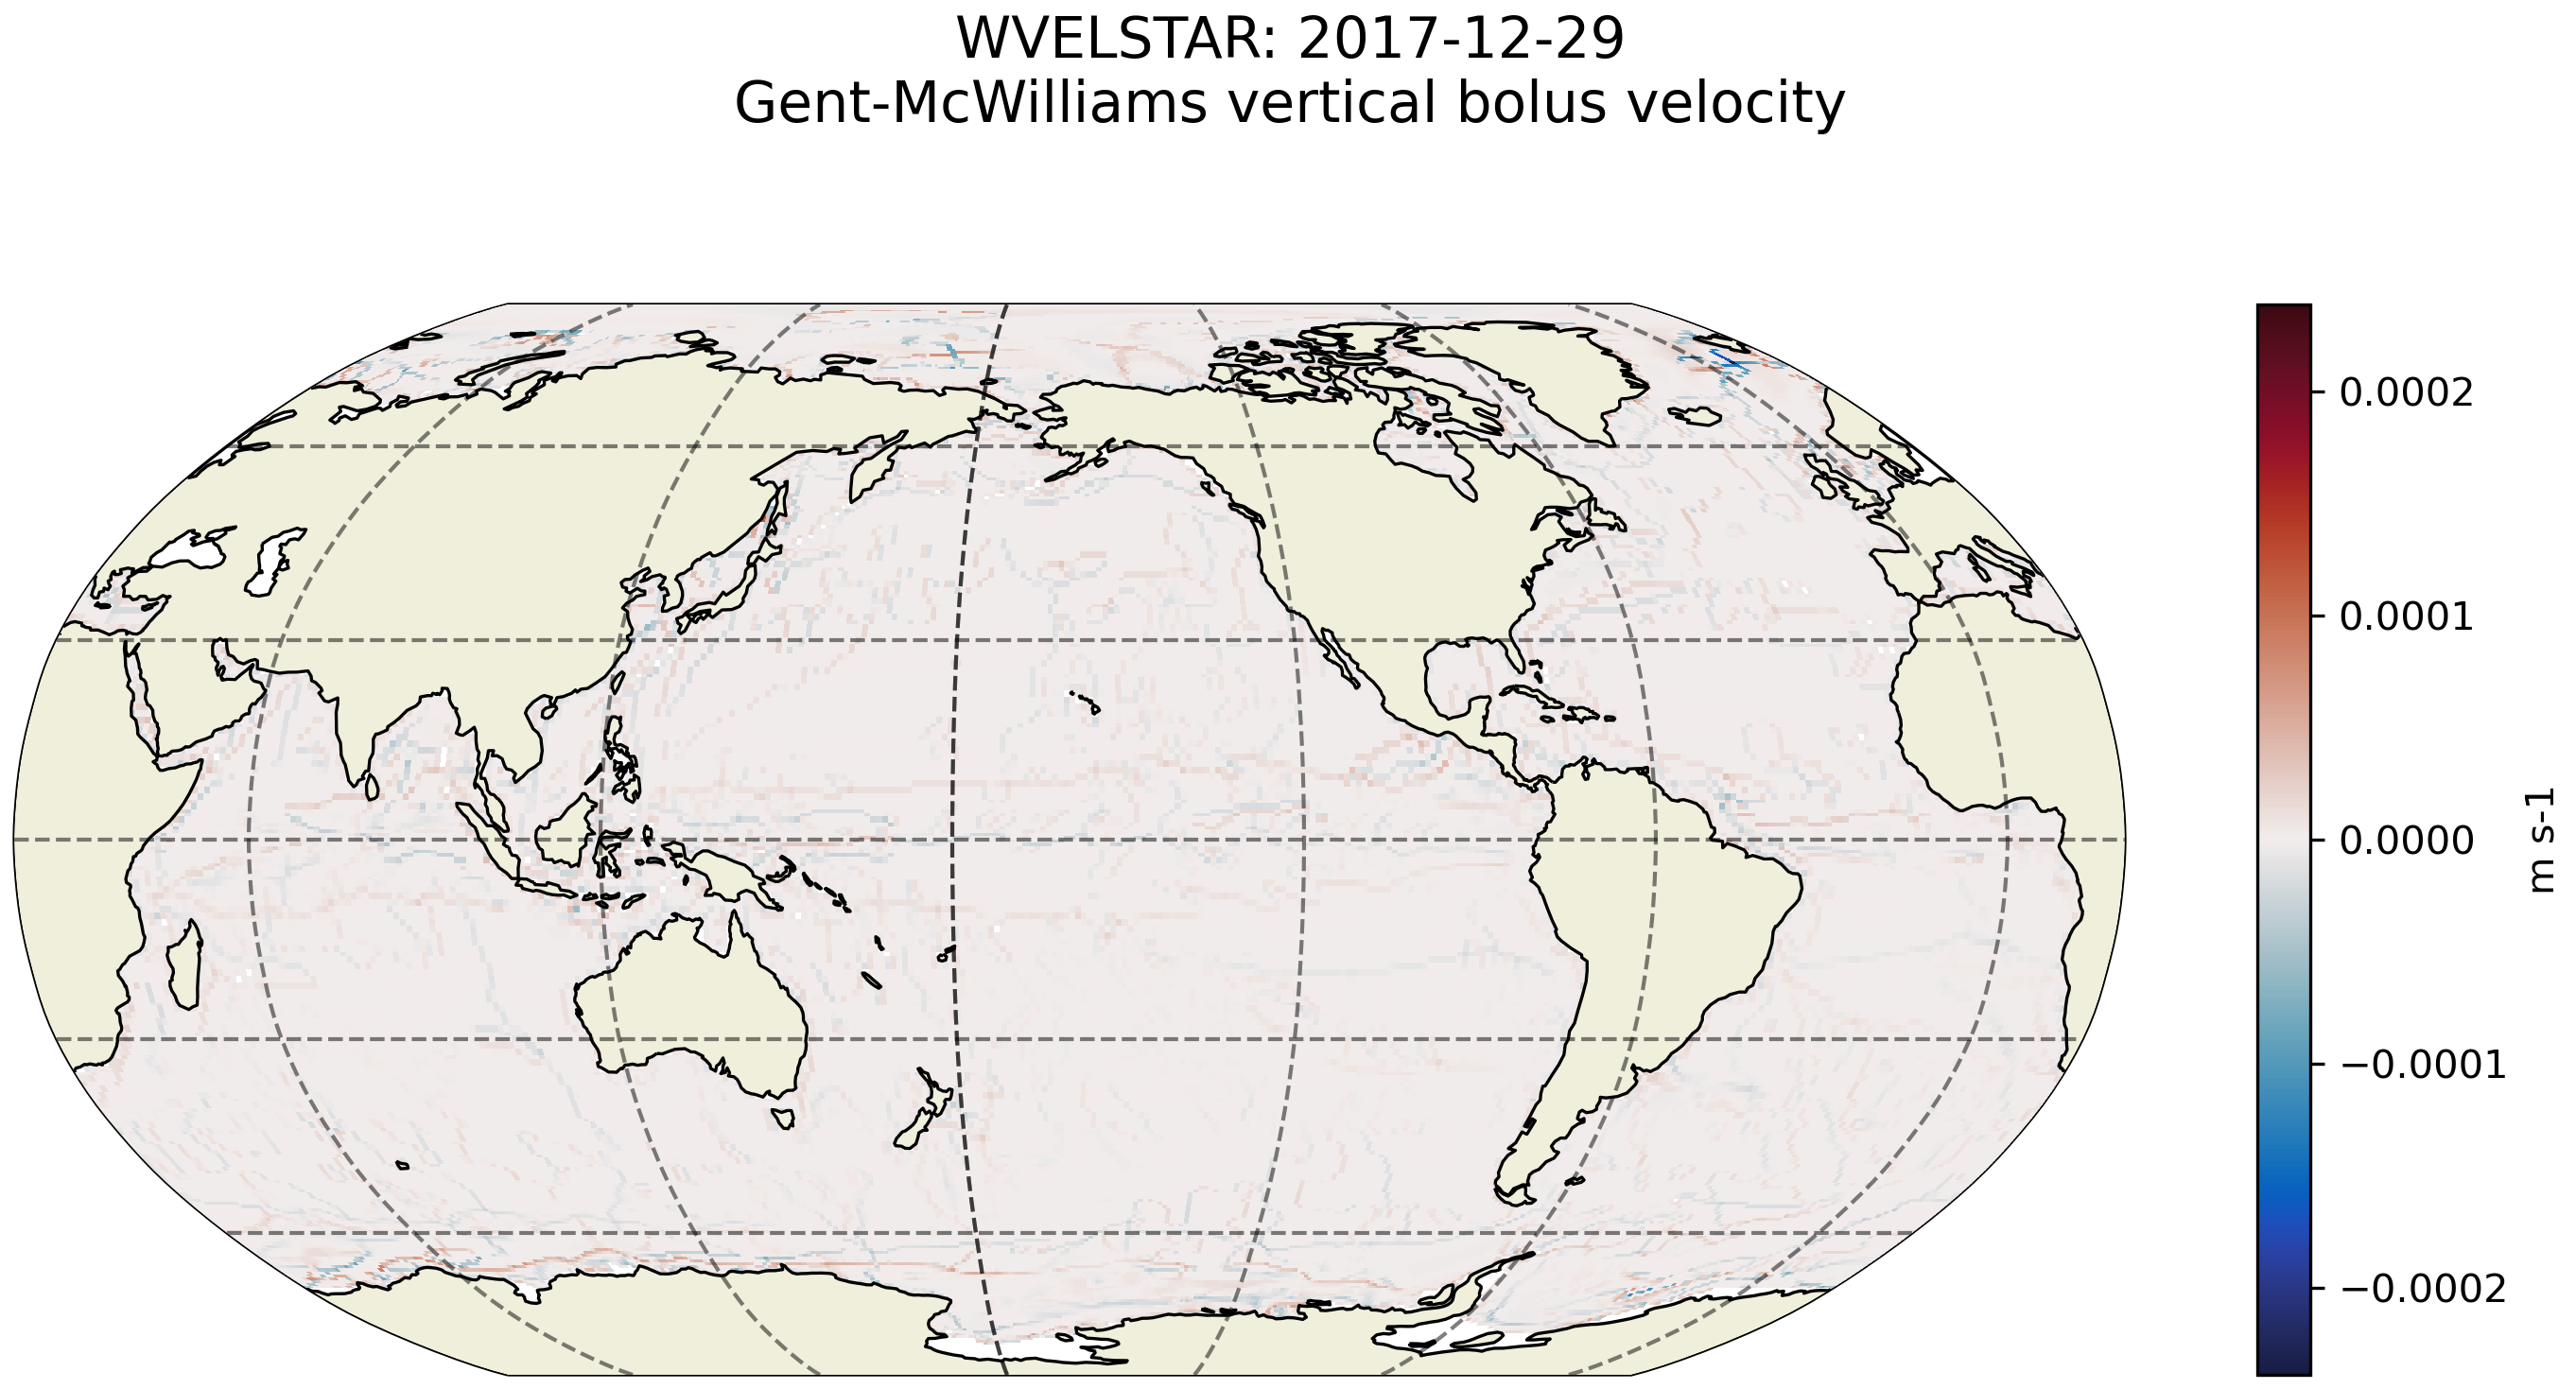
\includegraphics[width=\textwidth]{../images/plots/latlon_plots/Gent-McWilliams_Ocean_Bolus_Velocity/WVELSTAR.png}
\caption{Dataset: OCEAN\_BOLUS\_VELOCITY Variable: WVELSTAR}
\label{tab:table-OCEAN_BOLUS_VELOCITY_WVELSTAR-Plot}
\end{figure}
\pagebreak
\subsection{Latlon NetCDF OCEAN\_BOTTOM\_PRESSURE}
\newp
\begin{longtable}{|p{0.1\textwidth}|p{0.5\textwidth}|}
\caption{Variables in the dataset OCEAN\_BOTTOM\_PRESSURE}
\label{tab:table-OCEAN_BOTTOM_PRESSURE-fields} \\ 
\hline \endhead \hline \endfoot
\rowcolor{lightgray} \textbf{Dataset:} & \textbf{OCEAN\_BOTTOM\_PRESSURE} \\ \hline
Field: &OBP \\ \hline
Field: &OBPGMAP \\ \hline
\end{longtable}

\pagebreak
\subsubsection{Latlon Variable OBP}
\begin{longtable}{|p{0.06\textwidth}|p{0.41\textwidth}|p{0.39\textwidth}|p{0.06\textwidth}|}
\caption{CDL description of OCEAN\_BOTTOM\_PRESSURE's OBP variable}
\label{tab:table-OCEAN_BOTTOM_PRESSURE_OBP} \\ 
\hline \endhead \hline \endfoot
\rowcolor{lightgray} \textbf{Storage Type} & \textbf{Variable Name} & \textbf{Description} & \textbf{Unit} \\ \hline
float32 & OBP & Ocean bottom pressure given as equivalent water thickness & m \\ \hline
\rowcolor{lightgray}  \multicolumn{4}{|p{1.00\textwidth}|}{\textbf{CDL Description}} \\ \hline
\multicolumn{4}{|p{1.00\textwidth}|}{\makecell{\parbox{1\textwidth}{float32 OBP(time, latitude, longitude)\\
\hspace*{0.5cm}OBP: \_FillValue = 9.96921e+36\\
\hspace*{0.5cm}OBP: coverage\_content\_type = modelResult\\
\hspace*{0.5cm}OBP: long\_name = Ocean bottom pressure given as equivalent water thickness\\
\hspace*{0.5cm}OBP: units = m\\
\hspace*{0.5cm}OBP: coordinates = time\\
\hspace*{0.5cm}OBP: valid\_min = : 2.544442892074585\\
\hspace*{0.5cm}OBP: valid\_max = 72.1243667602539}}} \\ \hline
\rowcolor{lightgray} \multicolumn{4}{|p{1.00\textwidth}|}{\textbf{Comments}} \\ \hline
\multicolumn{4}{|p{1\textwidth}|}{OBP excludes the contribution from global mean atmospheric pressure and is therefore suitable for comparisons with GRACE data products. OBP is calculated as follows. First, we calculate ocean hydrostatic bottom pressure anomaly, PHIBOT, with PHIBOT = p\_b/rhoConst - gH(t), where p\_b = model ocean hydrostatic bottom pressure, rhoConst = reference density (1029 kg m-3), g is acceleration due to gravity (9.81 m s-2), and H(t) is model depth at time t. Then, OBP = PHIBOT/g + corrections for i) global mean steric sea level changes related to density changes in the Boussinesq volume-conserving model (Greatbatch correction, see sterGloH) and ii) global mean atmospheric pressure variations. Use OBP for comparisons with ocean bottom pressure data products that have been corrected for global mean atmospheric pressure variations. GRACE data typically ARE corrected for global mean atmospheric pressure variations. In contrast, ocean bottom pressure gauge data typically ARE NOT corrected for global mean atmospheric pressure variations.} \\ \hline
\end{longtable}

\begin{figure}[H]
\centering
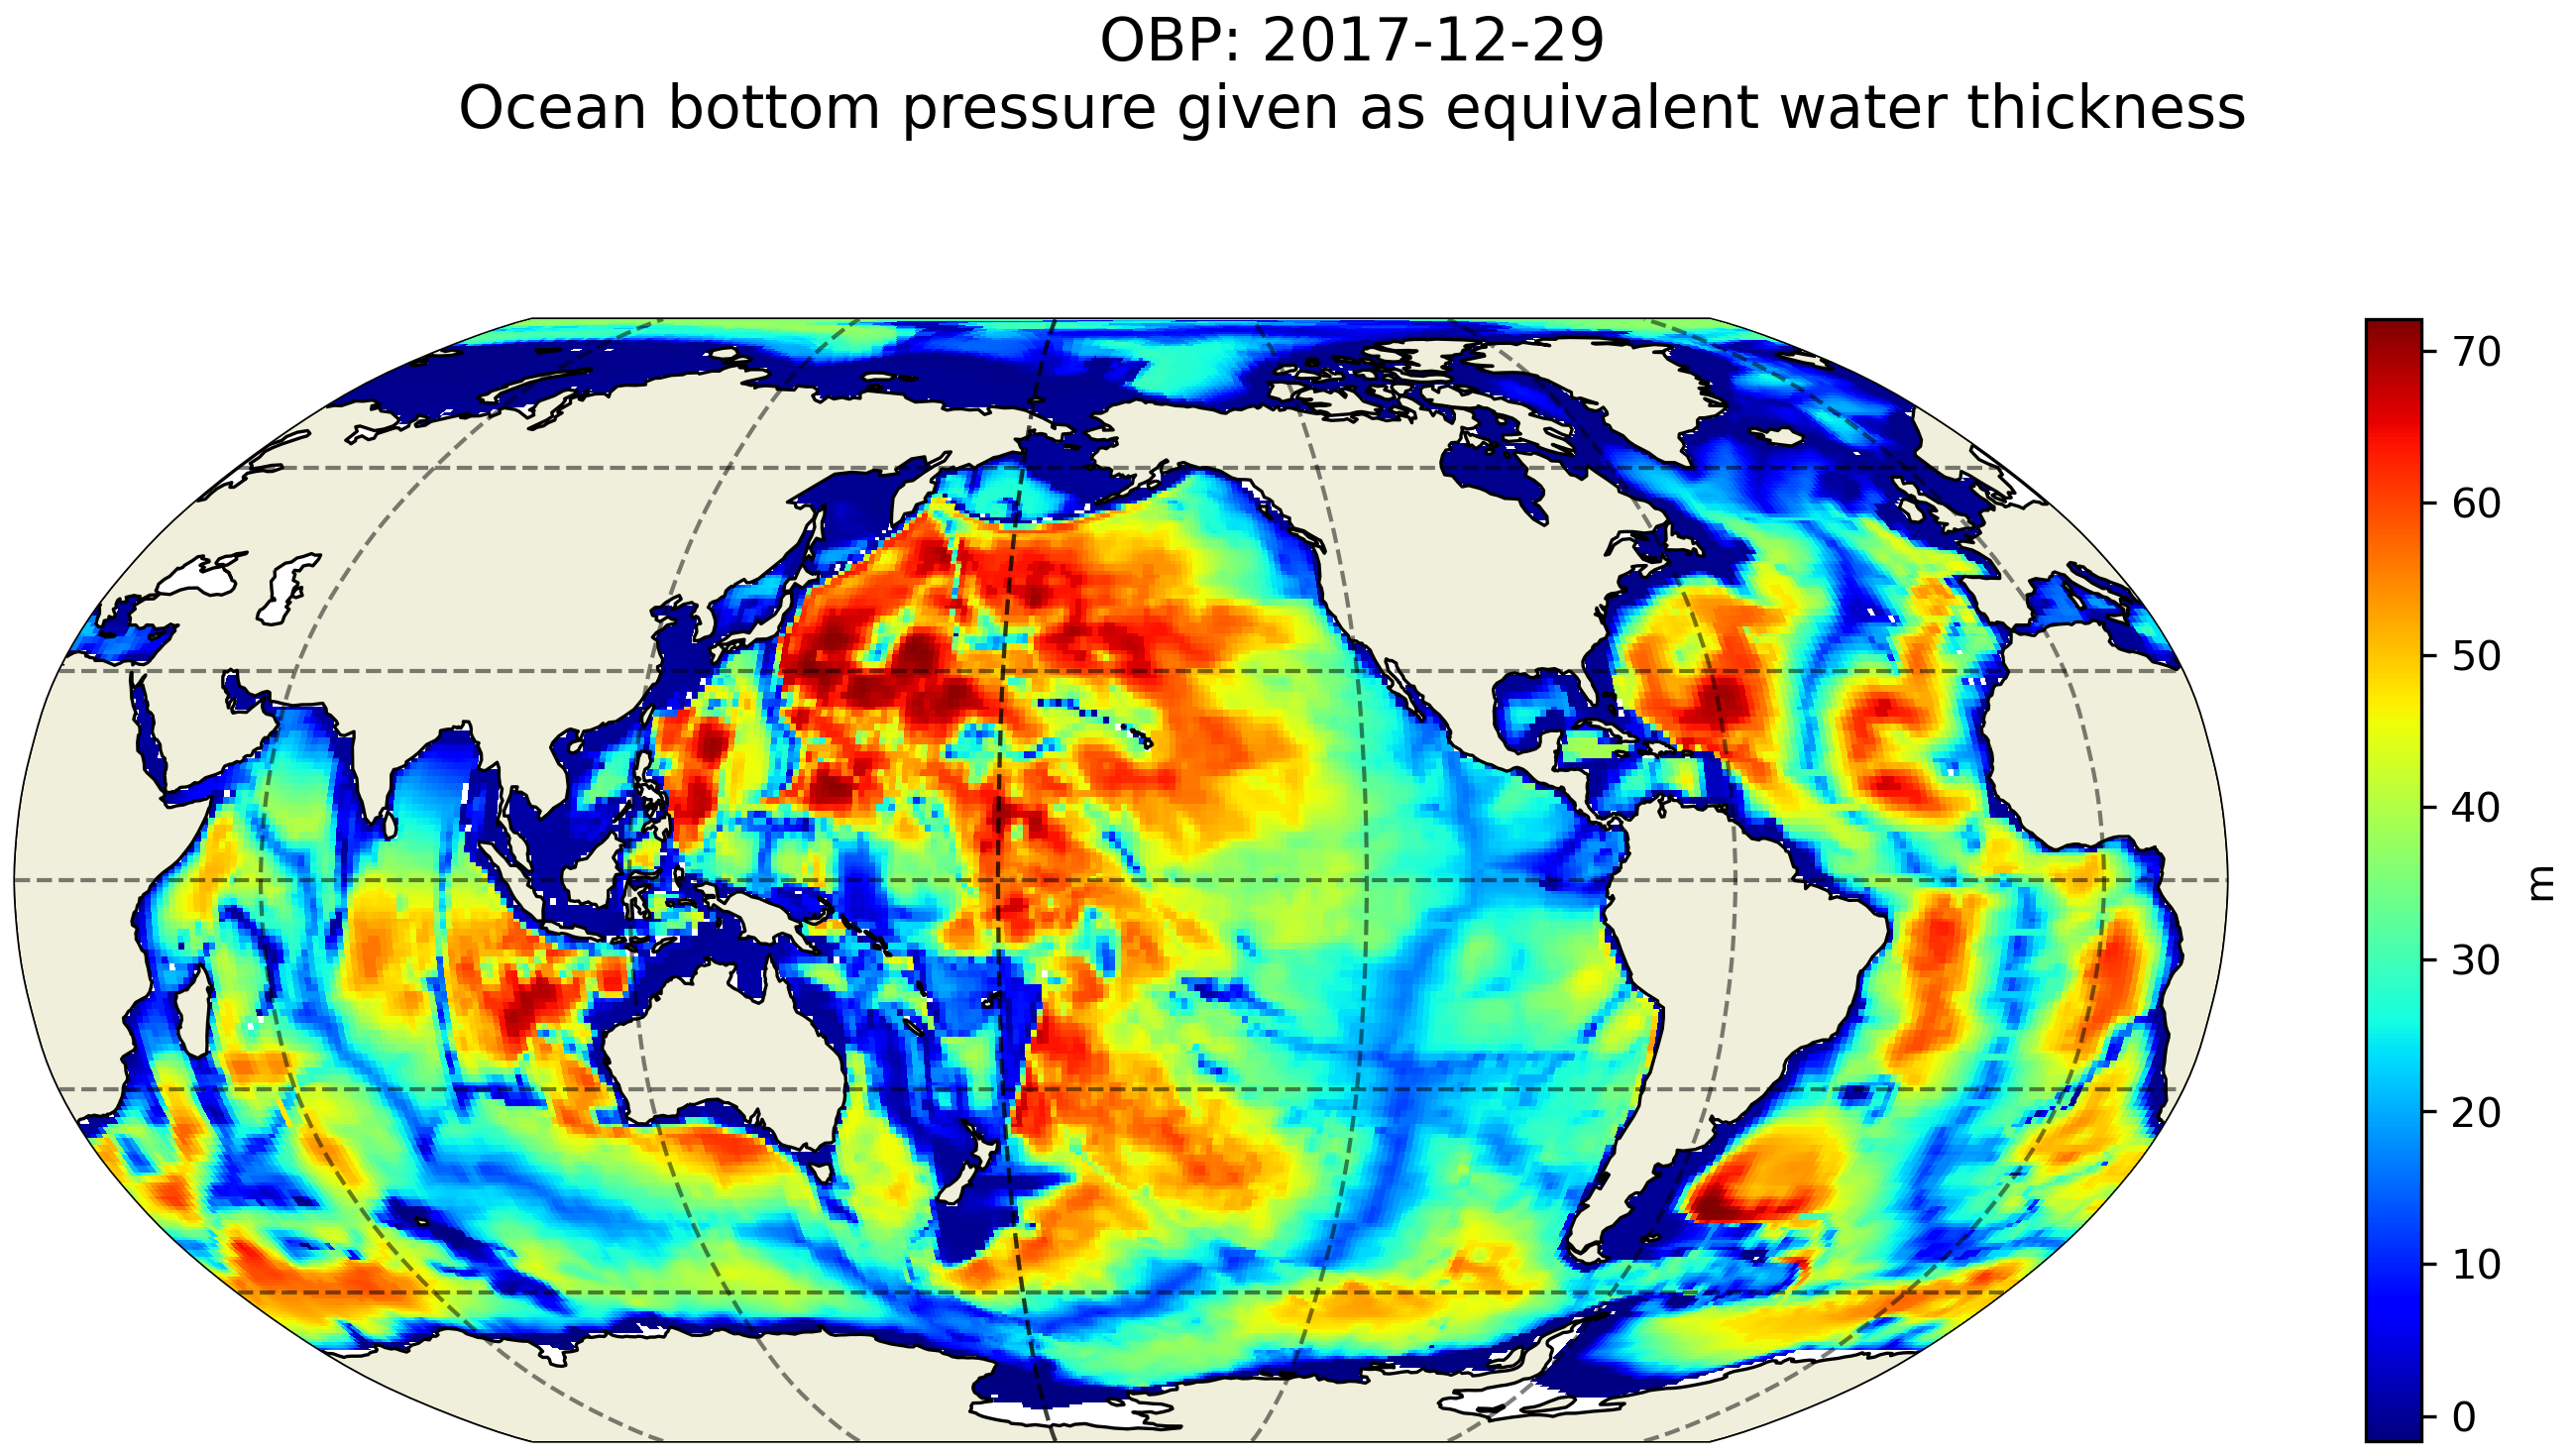
\includegraphics[width=\textwidth]{../images/plots/latlon_plots/Ocean_Bottom_Pressure/OBP.png}
\caption{Dataset: OCEAN\_BOTTOM\_PRESSURE Variable: OBP}
\label{tab:table-OCEAN_BOTTOM_PRESSURE_OBP-Plot}
\end{figure}
\pagebreak
\subsubsection{Latlon Variable OBPGMAP}
\begin{longtable}{|p{0.06\textwidth}|p{0.41\textwidth}|p{0.39\textwidth}|p{0.06\textwidth}|}
\caption{CDL description of OCEAN\_BOTTOM\_PRESSURE's OBPGMAP variable}
\label{tab:table-OCEAN_BOTTOM_PRESSURE_OBPGMAP} \\ 
\hline \endhead \hline \endfoot
\rowcolor{lightgray} \textbf{Storage Type} & \textbf{Variable Name} & \textbf{Description} & \textbf{Unit} \\ \hline
float32 & OBPGMAP & Ocean bottom pressure given as equivalent water thickness, includes global mean atmospheric pressure & m \\ \hline
\rowcolor{lightgray}  \multicolumn{4}{|p{1.00\textwidth}|}{\textbf{CDL Description}} \\ \hline
\multicolumn{4}{|p{1.00\textwidth}|}{\makecell{\parbox{1\textwidth}{float32 OBPGMAP(time, latitude, longitude)\\
\hspace*{0.5cm}OBPGMAP: \_FillValue = 9.96921e+36\\
\hspace*{0.5cm}OBPGMAP: coverage\_content\_type = modelResult\\
\hspace*{0.5cm}OBPGMAP: long\_name = Ocean bottom pressure given as equivalent water thickness\\
includes global mean atmospheric pressure\\
\hspace*{0.5cm}OBPGMAP: units = m\\
\hspace*{0.5cm}OBPGMAP: coordinates = time\\
\hspace*{0.5cm}OBPGMAP: valid\_min = 7.395928859710693\\
\hspace*{0.5cm}OBPGMAP: valid\_max = 82.14805603027344}}} \\ \hline
\rowcolor{lightgray} \multicolumn{4}{|p{1.00\textwidth}|}{\textbf{Comments}} \\ \hline
\multicolumn{4}{|p{1\textwidth}|}{OBPGMAP includes the contribution from global mean atmospheric pressure and is therefore suitable for comparisons with ocean bottom pressure gauge data products. OBPGMAP is calculated as follows. First, we calculate ocean hydrostatic bottom pressure anomaly, PHIBOT, with PHIBOT = p\_b/rhoConst - gH(t), where p\_b = model ocean hydrostatic bottom pressure, rhoConst = reference density (1029 kg m-3), g is acceleration due to gravity (9.81 m s-2), and H(t) is model depth at time t. Then, OBPGMAP= PHIBOT/g + corrections for global mean steric sea level changes related to density changes in the Boussinesq volume-conserving model (Greatbatch correction, see sterGloH). Use OBPGMAP for comparisons with ocean bottom pressure data products that have NOT been corrected for global mean atmospheric pressure variations. GRACE data typically ARE corrected for global mean atmospheric pressure variations. In contrast, ocean bottom pressure gauge data typically ARE NOT corrected for global mean atmospheric pressure variations.} \\ \hline
\end{longtable}

\begin{figure}[H]
\centering
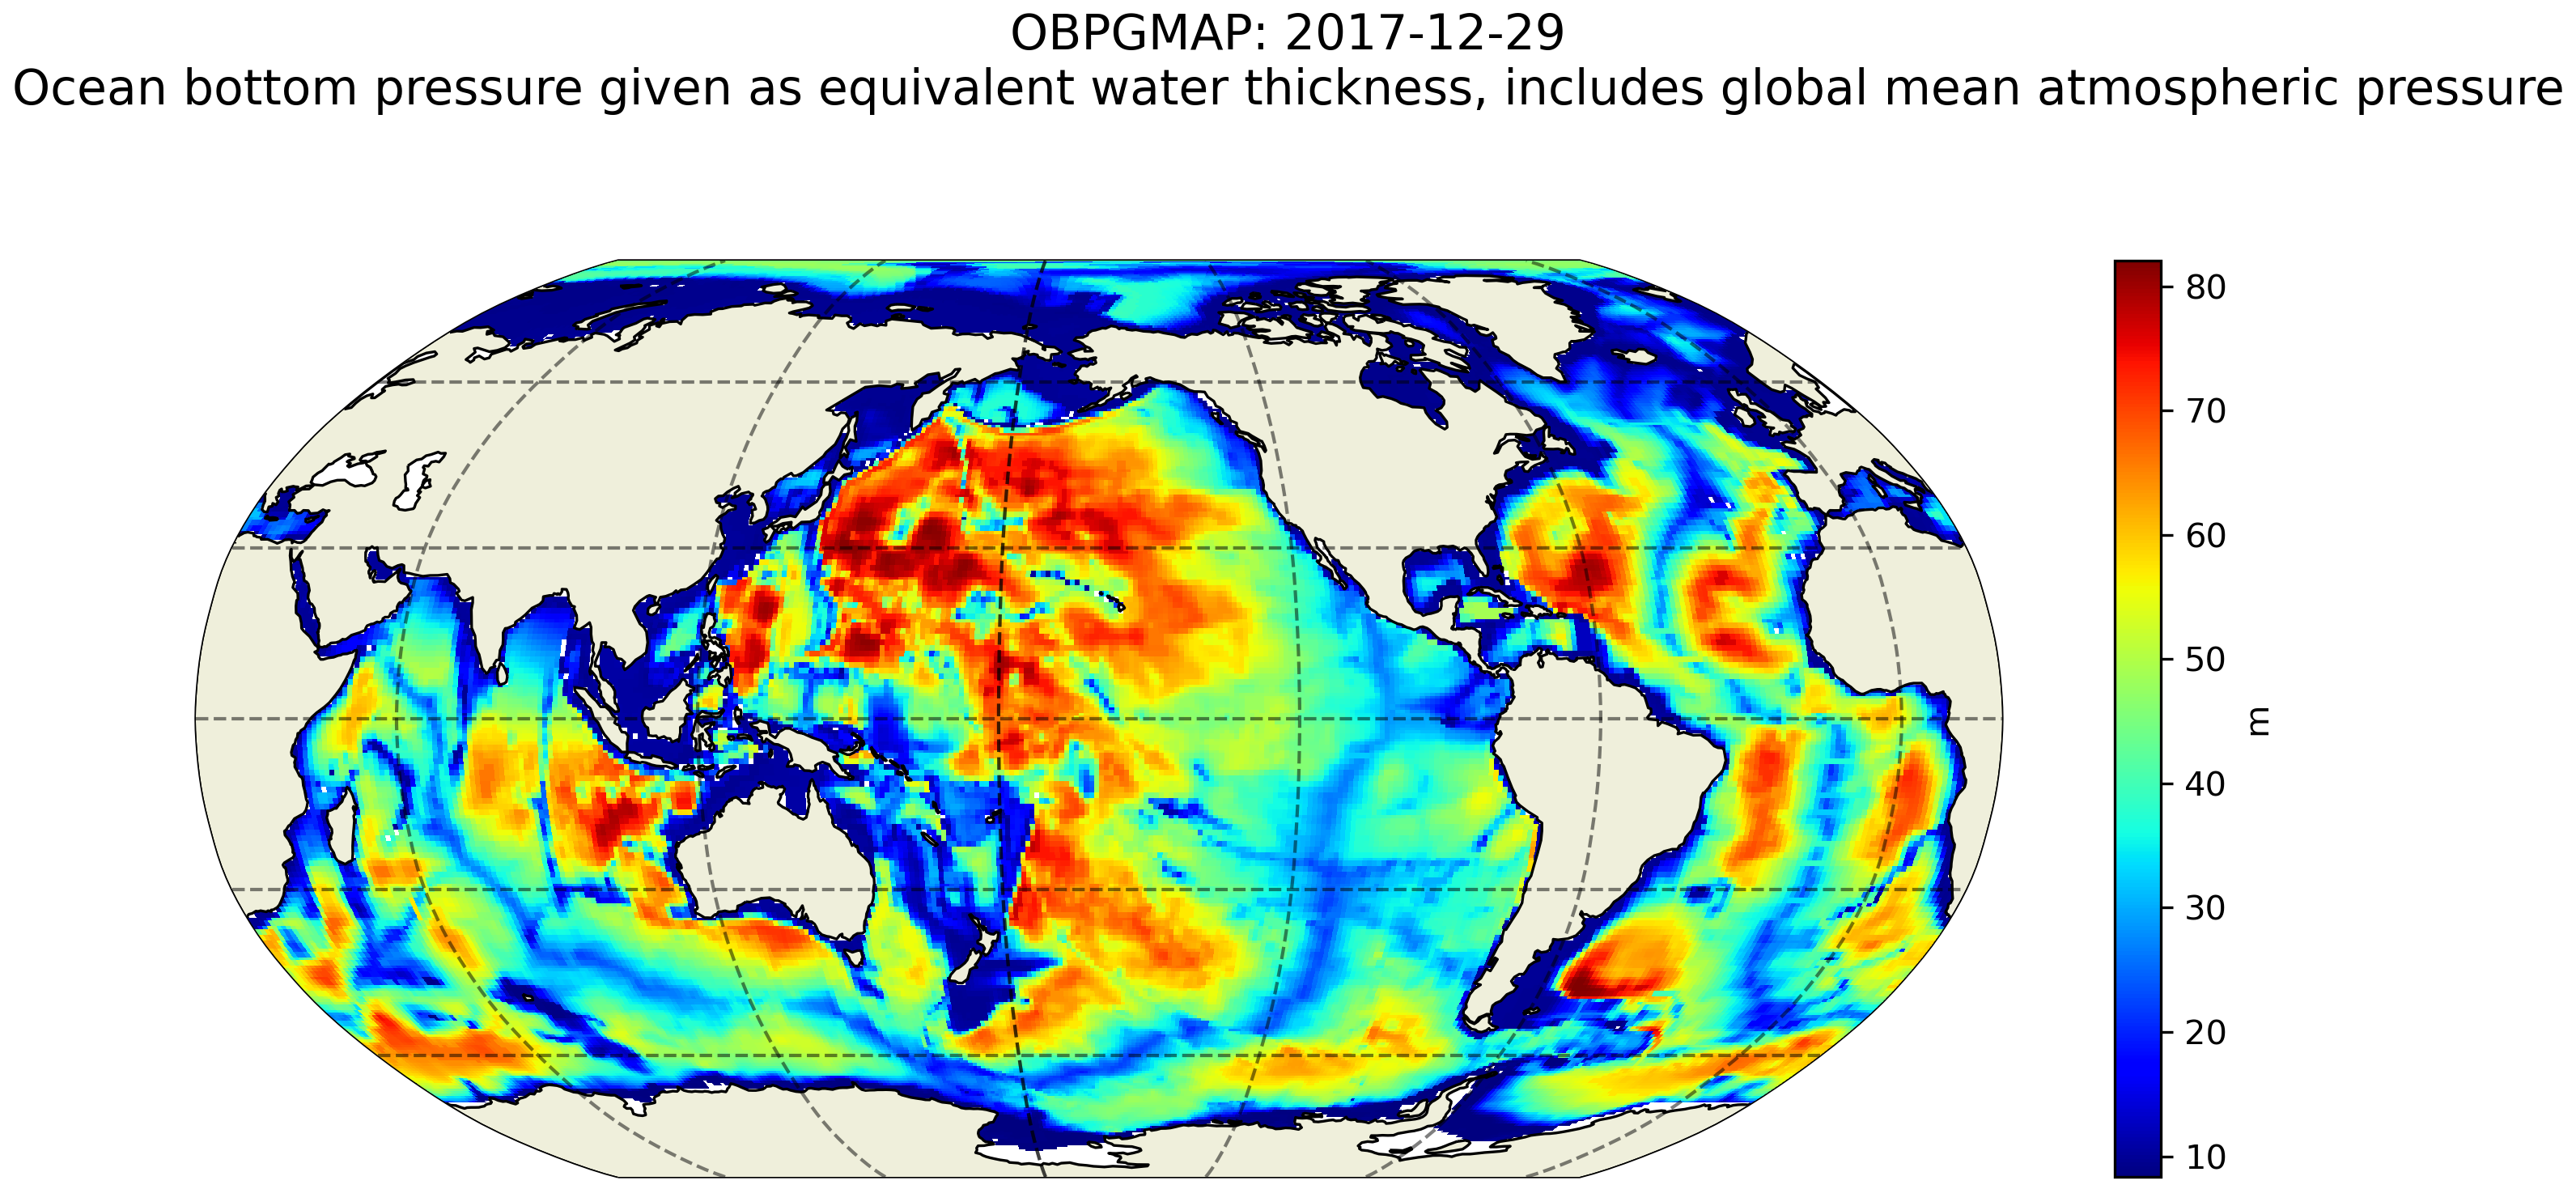
\includegraphics[width=\textwidth]{../images/plots/latlon_plots/Ocean_Bottom_Pressure/OBPGMAP.png}
\caption{Dataset: OCEAN\_BOTTOM\_PRESSURE Variable: OBPGMAP}
\label{tab:table-OCEAN_BOTTOM_PRESSURE_OBPGMAP-Plot}
\end{figure}
\pagebreak
\subsection{Latlon NetCDF OCEAN\_DENS\_STRAT\_PRESS}
\newp
\begin{longtable}{|p{0.1\textwidth}|p{0.5\textwidth}|}
\caption{Variables in the dataset OCEAN\_DENS\_STRAT\_PRESS}
\label{tab:table-OCEAN_DENS_STRAT_PRESS-fields} \\ 
\hline \endhead \hline \endfoot
\rowcolor{lightgray} \textbf{Dataset:} & \textbf{OCEAN\_DENS\_STRAT\_PRESS} \\ \hline
Field: &RHOAnoma \\ \hline
Field: &DRHODR \\ \hline
Field: &PHIHYD \\ \hline
\end{longtable}

\pagebreak
\subsubsection{Latlon Variable DRHODR}
\begin{longtable}{|p{0.06\textwidth}|p{0.41\textwidth}|p{0.39\textwidth}|p{0.06\textwidth}|}
\caption{CDL description of OCEAN\_DENS\_STRAT\_PRESS's DRHODR variable}
\label{tab:table-OCEAN_DENS_STRAT_PRESS_DRHODR} \\ 
\hline \endhead \hline \endfoot
\rowcolor{lightgray} \textbf{Storage Type} & \textbf{Variable Name} & \textbf{Description} & \textbf{Unit} \\ \hline
float32 & DRHODR & Density stratification & kg m-3 m-1 \\ \hline
\rowcolor{lightgray}  \multicolumn{4}{|p{1.00\textwidth}|}{\textbf{CDL Description}} \\ \hline
\multicolumn{4}{|p{1.00\textwidth}|}{\makecell{\parbox{1\textwidth}{float32 DRHODR(time, Z, latitude, longitude)\\
\hspace*{0.5cm}DRHODR: \_FillValue = 9.96921e+36\\
\hspace*{0.5cm}DRHODR: coverage\_content\_type = modelResult\\
\hspace*{0.5cm}DRHODR: long\_name = Density stratification\\
\hspace*{0.5cm}DRHODR: units = kg m: 3 m: 1\\
\hspace*{0.5cm}DRHODR: coordinates = time Z\\
\hspace*{0.5cm}DRHODR: valid\_min = : 0.8687265515327454\\
\hspace*{0.5cm}DRHODR: valid\_max = 0.011617615818977356}}} \\ \hline
\rowcolor{lightgray} \multicolumn{4}{|p{1.00\textwidth}|}{\textbf{Comments}} \\ \hline
\multicolumn{4}{|p{1\textwidth}|}{Density stratification: d(sigma) d z-1. Note: density computations are done with in-situ density. The vertical derivatives of in-situ density and locally-referenced potential density are identical  The equation of state is a modified UNESCO formula by Jackett and McDougall (1995), which uses the model variable potential temperature as input assuming a horizontally and temporally constant pressure of \$p\_0=-g 
ho\_\{0\} z\$.} \\ \hline
\end{longtable}

\begin{figure}[H]
\centering
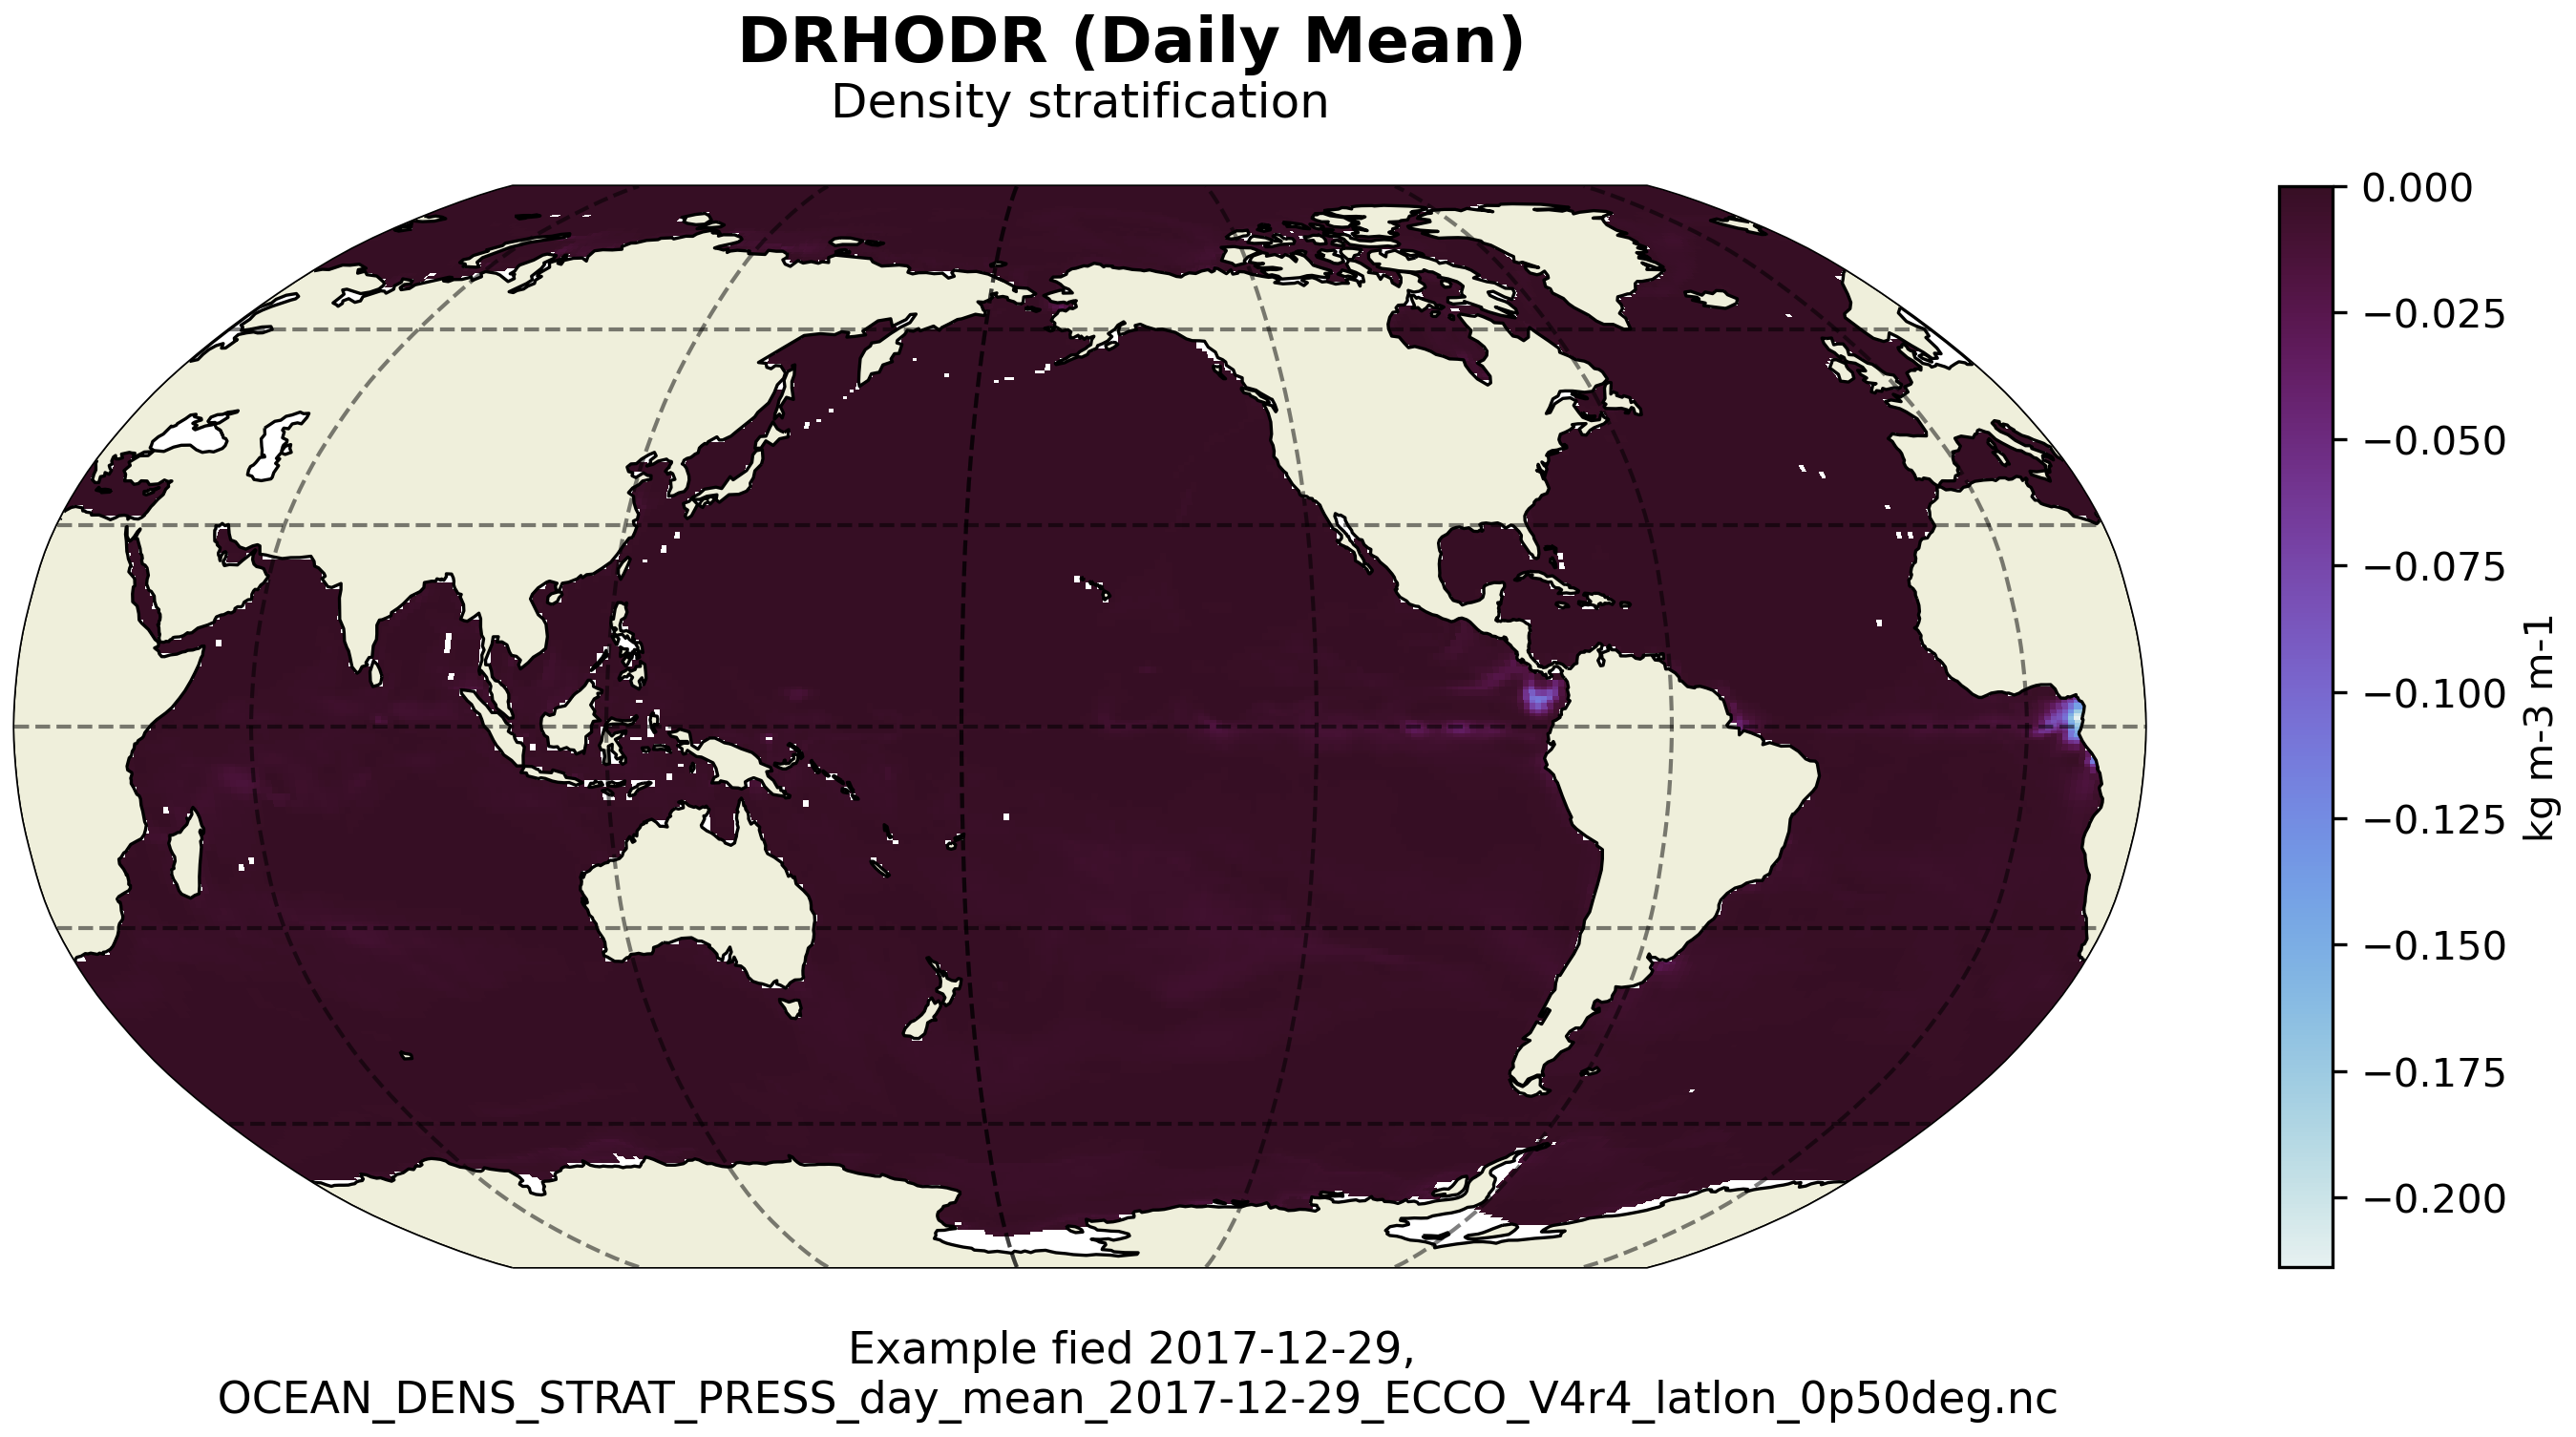
\includegraphics[width=\textwidth]{../images/plots/latlon_plots/Ocean_Density_Stratification_and_Hydrostatic_Pressure/DRHODR.png}
\caption{Dataset: OCEAN\_DENS\_STRAT\_PRESS Variable: DRHODR}
\label{tab:table-OCEAN_DENS_STRAT_PRESS_DRHODR-Plot}
\end{figure}
\pagebreak
\subsubsection{Latlon Variable PHIHYD}
\begin{longtable}{|p{0.06\textwidth}|p{0.41\textwidth}|p{0.39\textwidth}|p{0.06\textwidth}|}
\caption{CDL description of OCEAN\_DENS\_STRAT\_PRESS's PHIHYD variable}
\label{tab:table-OCEAN_DENS_STRAT_PRESS_PHIHYD} \\ 
\hline \endhead \hline \endfoot
\rowcolor{lightgray} \textbf{Storage Type} & \textbf{Variable Name} & \textbf{Description} & \textbf{Unit} \\ \hline
float32 & PHIHYD & Ocean hydrostatic pressure anomaly & m2 s-2 \\ \hline
\rowcolor{lightgray}  \multicolumn{4}{|p{1.00\textwidth}|}{\textbf{CDL Description}} \\ \hline
\multicolumn{4}{|p{1.00\textwidth}|}{\makecell{\parbox{1\textwidth}{float32 PHIHYD(time, Z, latitude, longitude)\\
\hspace*{0.5cm}PHIHYD: \_FillValue = 9.96921e+36\\
\hspace*{0.5cm}PHIHYD: coverage\_content\_type = modelResult\\
\hspace*{0.5cm}PHIHYD: long\_name = Ocean hydrostatic pressure anomaly\\
\hspace*{0.5cm}PHIHYD: units = m2 s: 2\\
\hspace*{0.5cm}PHIHYD: coordinates = time Z\\
\hspace*{0.5cm}PHIHYD: valid\_min = 74.71473693847656\\
\hspace*{0.5cm}PHIHYD: valid\_max = 783.9188232421875}}} \\ \hline
\rowcolor{lightgray} \multicolumn{4}{|p{1.00\textwidth}|}{\textbf{Comments}} \\ \hline
\multicolumn{4}{|p{1\textwidth}|}{PHIHYD = p(k) / rhoConst - g z*(k,t), where p = hydrostatic ocean pressure at depth level k, rhoConst = reference density (1029 kg m-3), g is acceleration due to gravity (9.81 m s-2), and z*(k,t) is model depth at level k and time t. Units: p:[kg m-1 s-2], rhoConst:[kg m-3], g:[m s-2], H(t):[m]. Note: includes atmospheric pressure loading. Quantity referred to in some contexts as hydrostatic pressure anomaly. PHIBOT accounts for the model's time-varying grid cell thickness (z* coordinate system). See PHIHYDcR for hydrostatic pressure potential anomaly calculated using time-invariant grid cell thicknesses. PHIHYD is NOT corrected for global mean steric sea level changes related to density changes in the Boussinesq volume-conserving model (Greatbatch correction, see sterGloH). } \\ \hline
\end{longtable}

\begin{figure}[H]
\centering
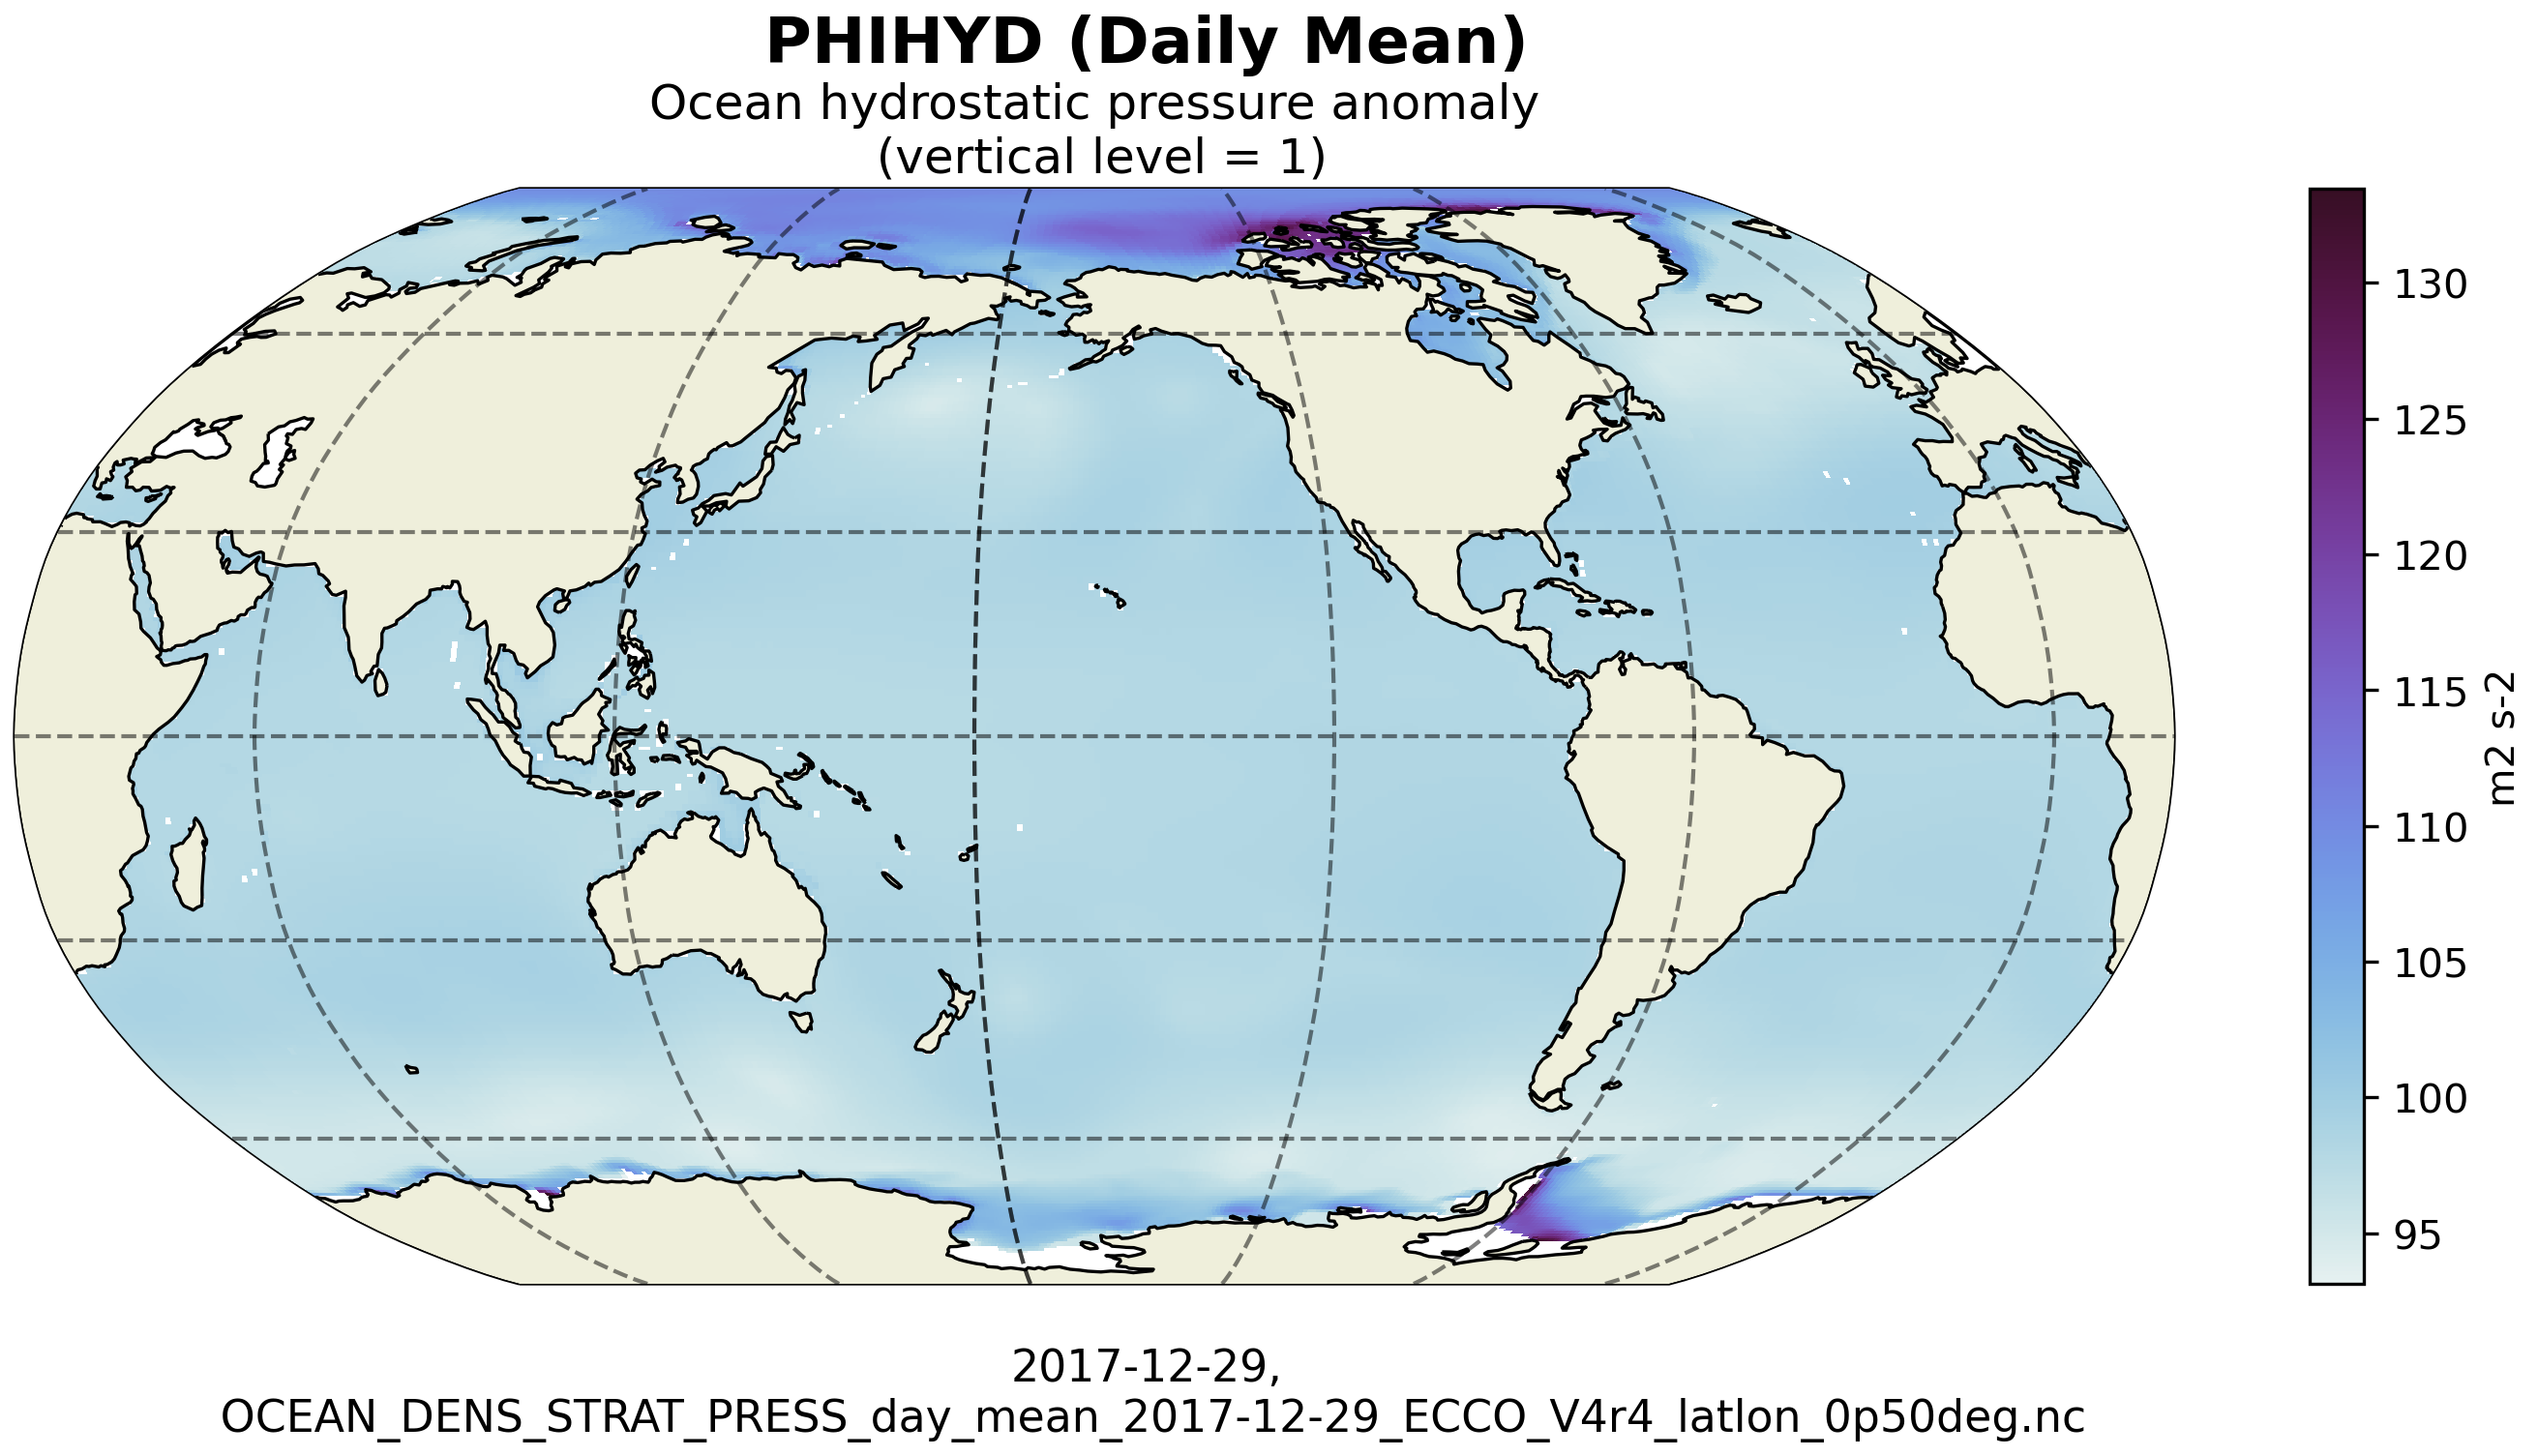
\includegraphics[width=\textwidth]{../images/plots/latlon_plots/Ocean_Density_Stratification_and_Hydrostatic_Pressure/PHIHYD.png}
\caption{Dataset: OCEAN\_DENS\_STRAT\_PRESS Variable: PHIHYD}
\label{tab:table-OCEAN_DENS_STRAT_PRESS_PHIHYD-Plot}
\end{figure}
\pagebreak
\subsubsection{Latlon Variable RHOAnoma}
\begin{longtable}{|p{0.06\textwidth}|p{0.41\textwidth}|p{0.39\textwidth}|p{0.06\textwidth}|}
\caption{CDL description of OCEAN\_DENS\_STRAT\_PRESS's RHOAnoma variable}
\label{tab:table-OCEAN_DENS_STRAT_PRESS_RHOAnoma} \\ 
\hline \endhead \hline \endfoot
\rowcolor{lightgray} \textbf{Storage Type} & \textbf{Variable Name} & \textbf{Description} & \textbf{Unit} \\ \hline
float32 & RHOAnoma & In-situ seawater density anomaly & kg m-3 \\ \hline
\rowcolor{lightgray}  \multicolumn{4}{|p{1.00\textwidth}|}{\textbf{CDL Description}} \\ \hline
\multicolumn{4}{|p{1.00\textwidth}|}{\makecell{\parbox{1\textwidth}{float32 RHOAnoma(time, Z, latitude, longitude)\\
\hspace*{0.5cm}RHOAnoma: \_FillValue = 9.96921e+36\\
\hspace*{0.5cm}RHOAnoma: coverage\_content\_type = modelResult\\
\hspace*{0.5cm}RHOAnoma: long\_name = In: situ seawater density anomaly\\
\hspace*{0.5cm}RHOAnoma: units = kg m: 3\\
\hspace*{0.5cm}RHOAnoma: coordinates = time Z\\
\hspace*{0.5cm}RHOAnoma: valid\_min = : 19.919862747192383\\
\hspace*{0.5cm}RHOAnoma: valid\_max = 25.540647506713867}}} \\ \hline
\rowcolor{lightgray} \multicolumn{4}{|p{1.00\textwidth}|}{\textbf{Comments}} \\ \hline
\multicolumn{4}{|p{1\textwidth}|}{In-situ seawater density anomaly relative to the reference density, rhoConst. rhoConst = 1029 kg m-3} \\ \hline
\end{longtable}

\begin{figure}[H]
\centering
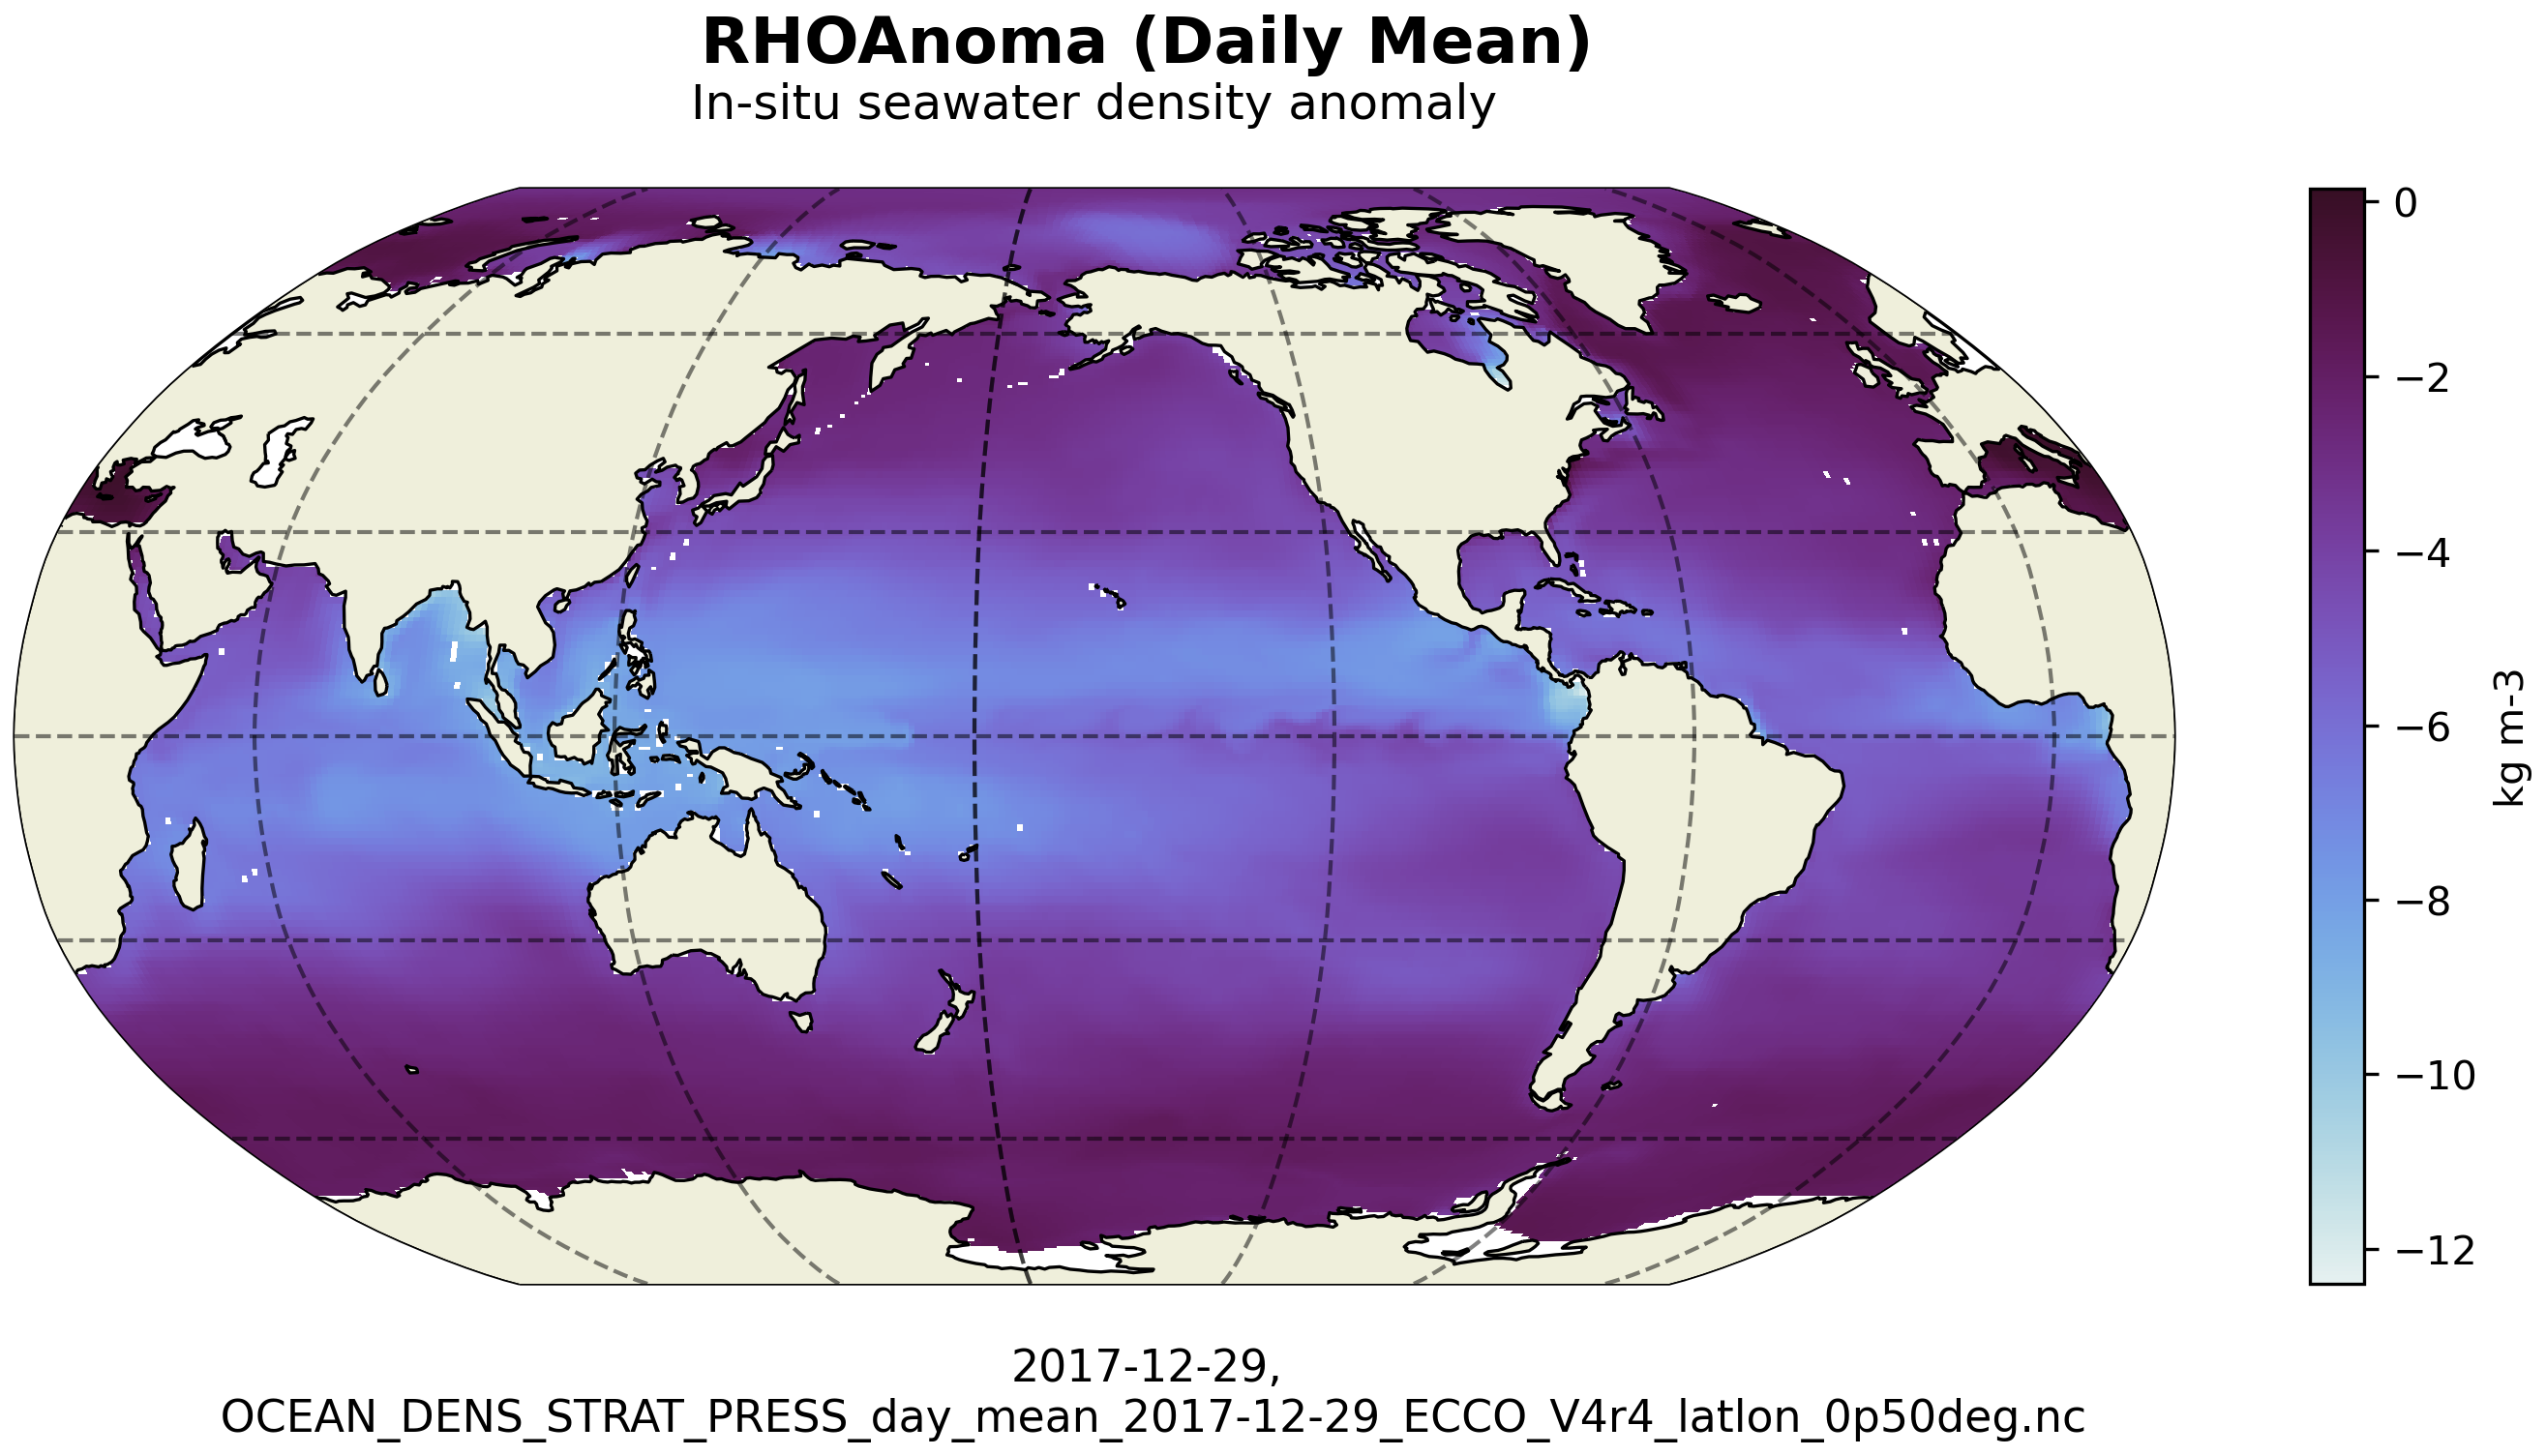
\includegraphics[width=\textwidth]{../images/plots/latlon_plots/Ocean_Density_Stratification_and_Hydrostatic_Pressure/RHOAnoma.png}
\caption{Dataset: OCEAN\_DENS\_STRAT\_PRESS Variable: RHOAnoma}
\label{tab:table-OCEAN_DENS_STRAT_PRESS_RHOAnoma-Plot}
\end{figure}
\pagebreak
\subsection{Latlon NetCDF OCEAN\_MIXED\_LAYER\_DEPTH}
\newp
\begin{longtable}{|p{0.1\textwidth}|p{0.5\textwidth}|}
\caption{Variables in the dataset OCEAN\_MIXED\_LAYER\_DEPTH}
\label{tab:table-OCEAN_MIXED_LAYER_DEPTH-fields} \\ 
\hline \endhead \hline \endfoot
\rowcolor{lightgray} \textbf{Dataset:} & \textbf{OCEAN\_MIXED\_LAYER\_DEPTH} \\ \hline
Field: &MXLDEPTH \\ \hline
\end{longtable}

\pagebreak
\subsubsection{Latlon Variable MXLDEPTH}
\begin{longtable}{|p{0.06\textwidth}|p{0.41\textwidth}|p{0.39\textwidth}|p{0.06\textwidth}|}
\caption{CDL description of OCEAN\_MIXED\_LAYER\_DEPTH's MXLDEPTH variable}
\label{tab:table-OCEAN_MIXED_LAYER_DEPTH_MXLDEPTH} \\ 
\hline \endhead \hline \endfoot
\rowcolor{lightgray} \textbf{Storage Type} & \textbf{Variable Name} & \textbf{Description} & \textbf{Unit} \\ \hline
float32 & MXLDEPTH & Mixed-layer depth diagnosed using the temperature difference criterion of Kara et al., 2000 & m \\ \hline
\rowcolor{lightgray}  \multicolumn{4}{|p{1.00\textwidth}|}{\textbf{CDL Description}} \\ \hline
\multicolumn{4}{|p{1.00\textwidth}|}{\makecell{\parbox{1\textwidth}{float32 MXLDEPTH(time, latitude, longitude)\\
\hspace*{0.5cm}MXLDEPTH: \_FillValue = 9.96921e+36\\
\hspace*{0.5cm}MXLDEPTH: coverage\_content\_type = modelResult\\
\hspace*{0.5cm}MXLDEPTH: long\_name = Mixed: layer depth diagnosed using the temperature difference criterion of Kara et al.\\
2000\\
\hspace*{0.5cm}MXLDEPTH: standard\_name = ocean\_mixed\_layer\_thickness\\
\hspace*{0.5cm}MXLDEPTH: units = m\\
\hspace*{0.5cm}MXLDEPTH: coordinates = time\\
\hspace*{0.5cm}MXLDEPTH: valid\_min = 5.000001430511475\\
\hspace*{0.5cm}MXLDEPTH: valid\_max = 5331.2001953125}}} \\ \hline
\rowcolor{lightgray} \multicolumn{4}{|p{1.00\textwidth}|}{\textbf{Comments}} \\ \hline
\multicolumn{4}{|p{1\textwidth}|}{Mixed-layer depth as determined by the depth where waters are first 0.8 degrees Celsius colder than the surface. See Kara et al. (JGR, 2000). . Note: the Kara et al. criterion may not be appropriate for some applications. If needed, mixed layer depth can be calculated using different criteria. See vertical density stratification (DRHODR) and density anomaly (RHOAnoma).} \\ \hline
\end{longtable}

\begin{figure}[H]
\centering
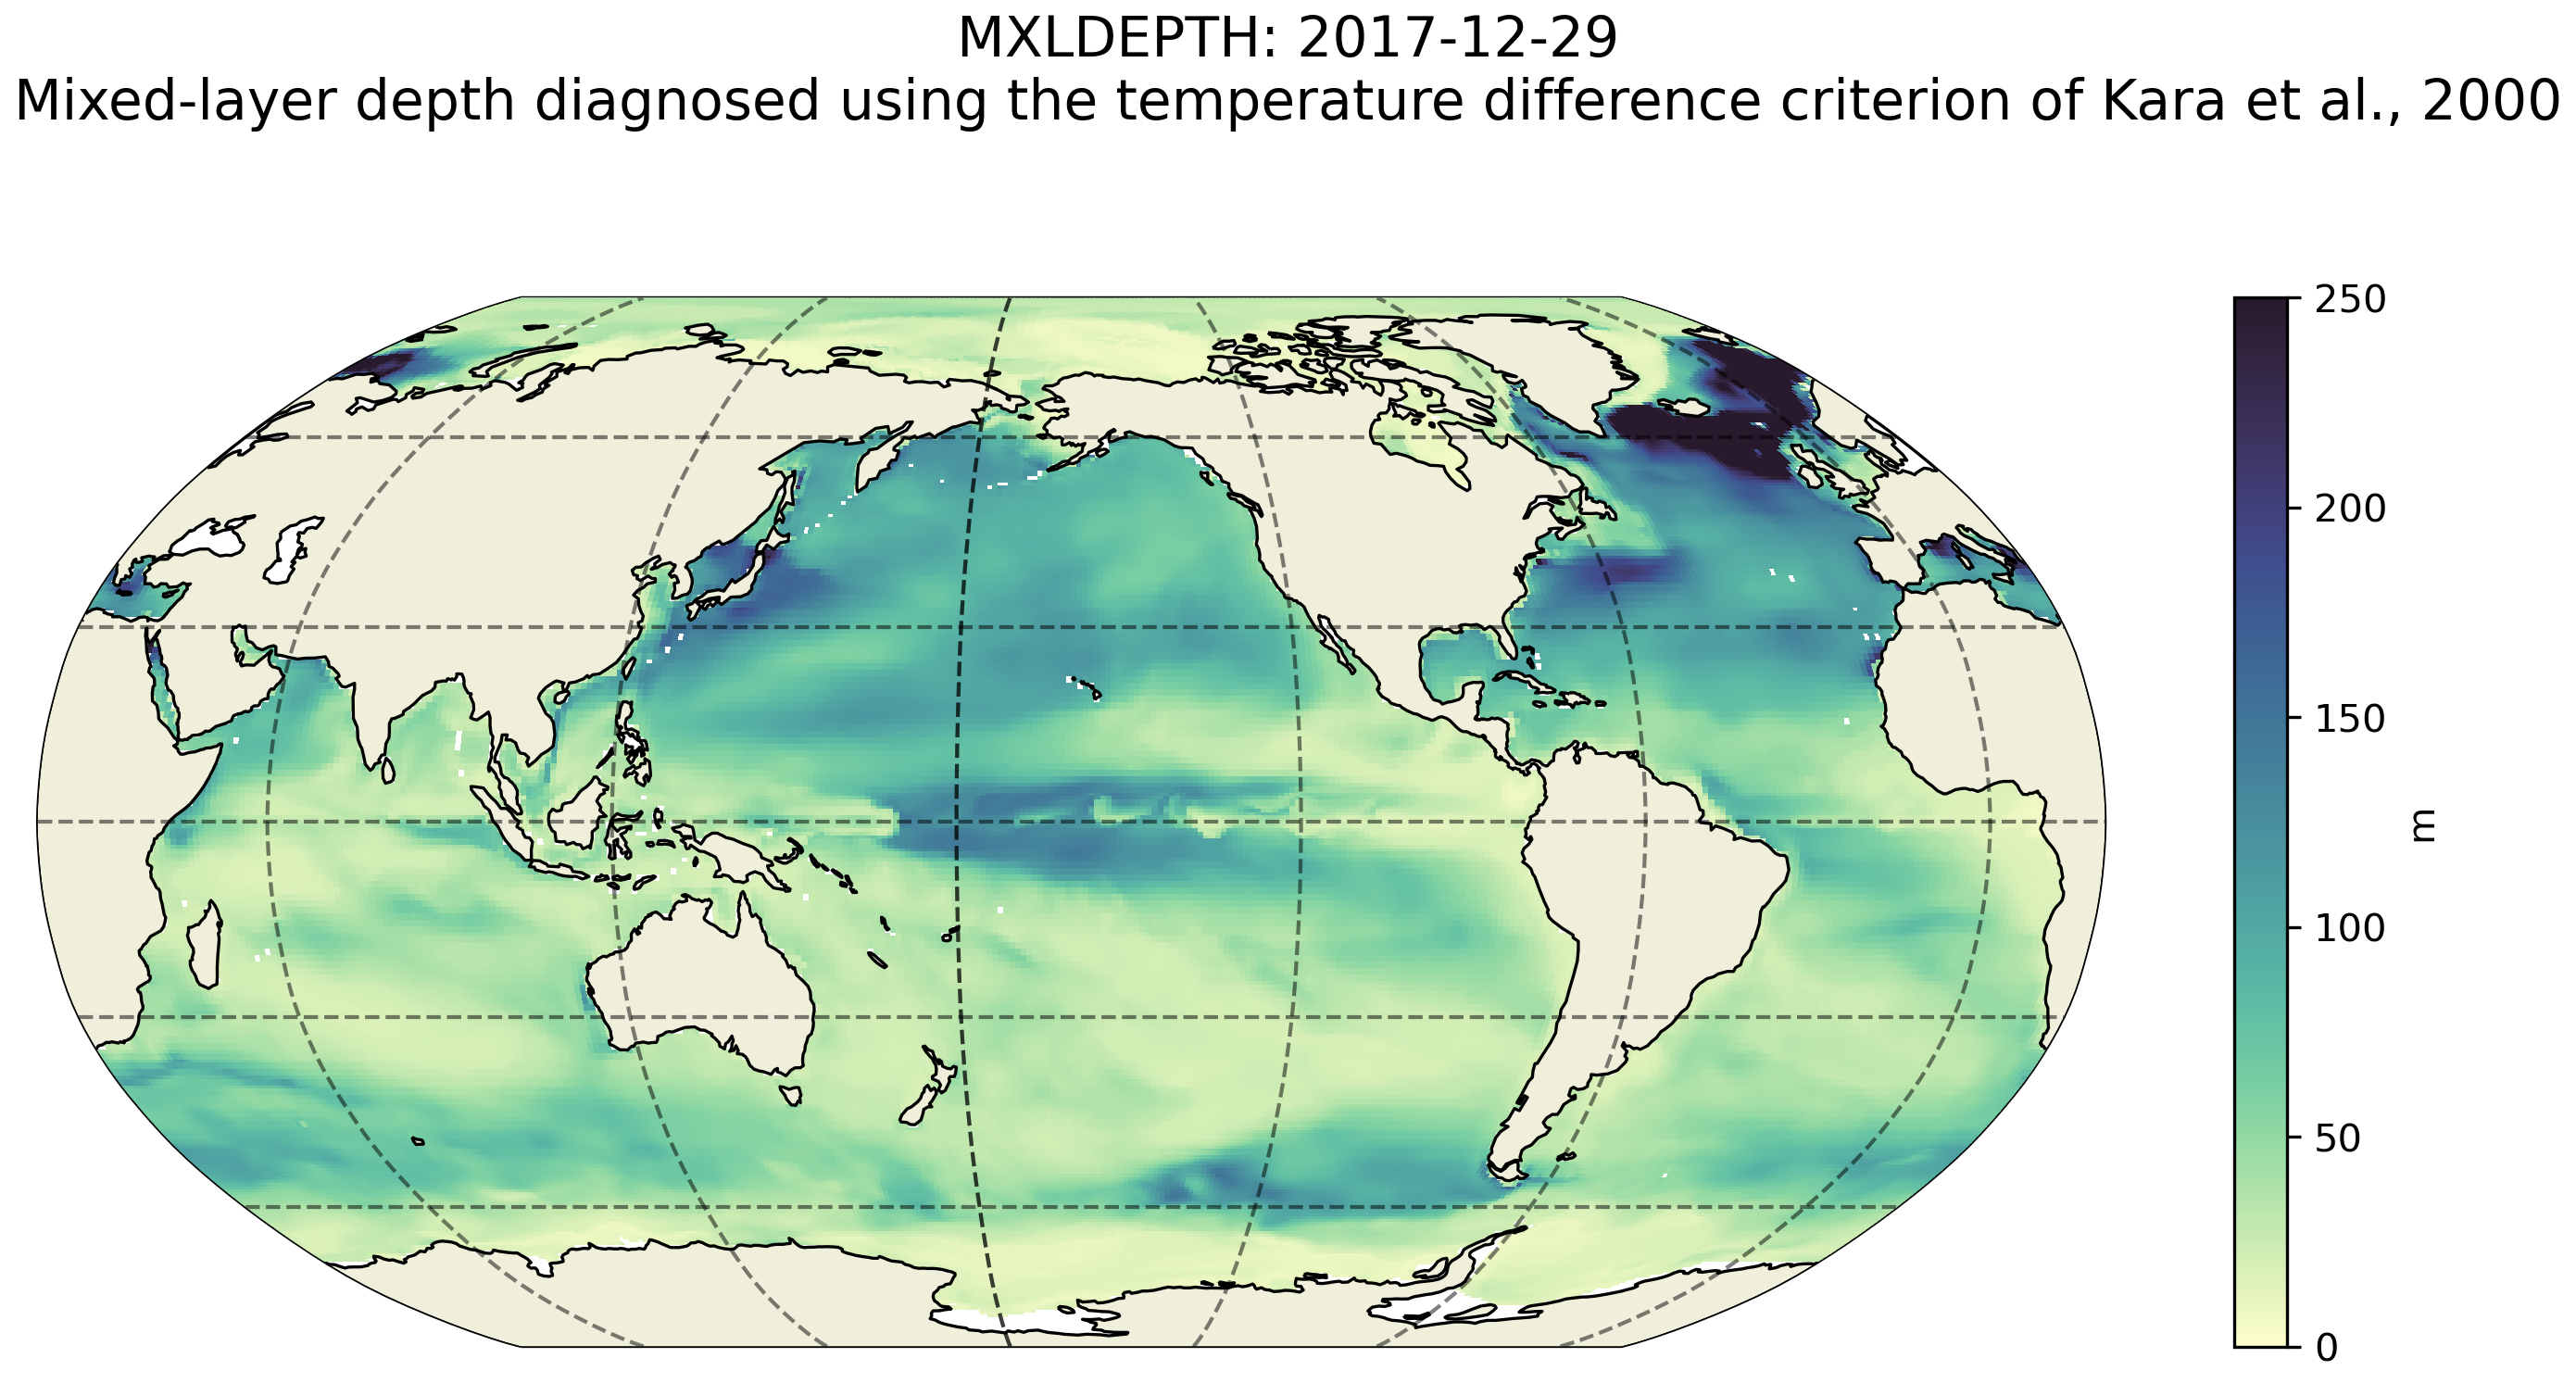
\includegraphics[width=\textwidth]{../images/plots/latlon_plots/Ocean_Mixed_Layer_Depth/MXLDEPTH.png}
\caption{Dataset: OCEAN\_MIXED\_LAYER\_DEPTH Variable: MXLDEPTH}
\label{tab:table-OCEAN_MIXED_LAYER_DEPTH_MXLDEPTH-Plot}
\end{figure}
\pagebreak
\subsection{Latlon NetCDF OCEAN\_TEMPERATURE\_SALINITY}
\newp
\begin{longtable}{|p{0.1\textwidth}|p{0.5\textwidth}|}
\caption{Variables in the dataset OCEAN\_TEMPERATURE\_SALINITY}
\label{tab:table-OCEAN_TEMPERATURE_SALINITY-fields} \\ 
\hline \endhead \hline \endfoot
\rowcolor{lightgray} \textbf{Dataset:} & \textbf{OCEAN\_TEMPERATURE\_SALINITY} \\ \hline
Field: &THETA \\ \hline
Field: &SALT \\ \hline
\end{longtable}

\pagebreak
\subsubsection{Latlon Variable SALT}
\begin{longtable}{|p{0.06\textwidth}|p{0.41\textwidth}|p{0.39\textwidth}|p{0.06\textwidth}|}
\caption{CDL description of OCEAN\_TEMPERATURE\_SALINITY's SALT variable}
\label{tab:table-OCEAN_TEMPERATURE_SALINITY_SALT} \\ 
\hline \endhead \hline \endfoot
\rowcolor{lightgray} \textbf{Storage Type} & \textbf{Variable Name} & \textbf{Description} & \textbf{Unit} \\ \hline
float32 & SALT & Salinity & 1e-3 \\ \hline
\rowcolor{lightgray}  \multicolumn{4}{|p{1.00\textwidth}|}{\textbf{CDL Description}} \\ \hline
\multicolumn{4}{|p{1.00\textwidth}|}{\makecell{\parbox{1\textwidth}{float32 SALT(time, Z, latitude, longitude)\\
\hspace*{0.5cm}SALT: \_FillValue = 9.96921e+36\\
\hspace*{0.5cm}SALT: coverage\_content\_type = modelResult\\
\hspace*{0.5cm}SALT: long\_name = Salinity\\
\hspace*{0.5cm}SALT: standard\_name = sea\_water\_salinity\\
\hspace*{0.5cm}SALT: units = 1e: 3\\
\hspace*{0.5cm}SALT: coordinates = time Z\\
\hspace*{0.5cm}SALT: valid\_min = 16.73577880859375\\
\hspace*{0.5cm}SALT: valid\_max = 41.321231842041016}}} \\ \hline
\rowcolor{lightgray} \multicolumn{4}{|p{1.00\textwidth}|}{\textbf{Comments}} \\ \hline
\multicolumn{4}{|p{1\textwidth}|}{Defined using CF convention 'Sea water salinity is the salt content of sea water, often on the Practical Salinity Scale of 1978. However, the unqualified term 'salinity' is generic and does not necessarily imply any particular method of calculation. The units of salinity are dimensionless and the units attribute should normally be given as 1e-3 or 0.001 i.e. parts per thousand.' see https://cfconventions.org/Data/cf-standard-names/73/build/cf-standard-name-table.html} \\ \hline
\end{longtable}

\begin{figure}[H]
\centering
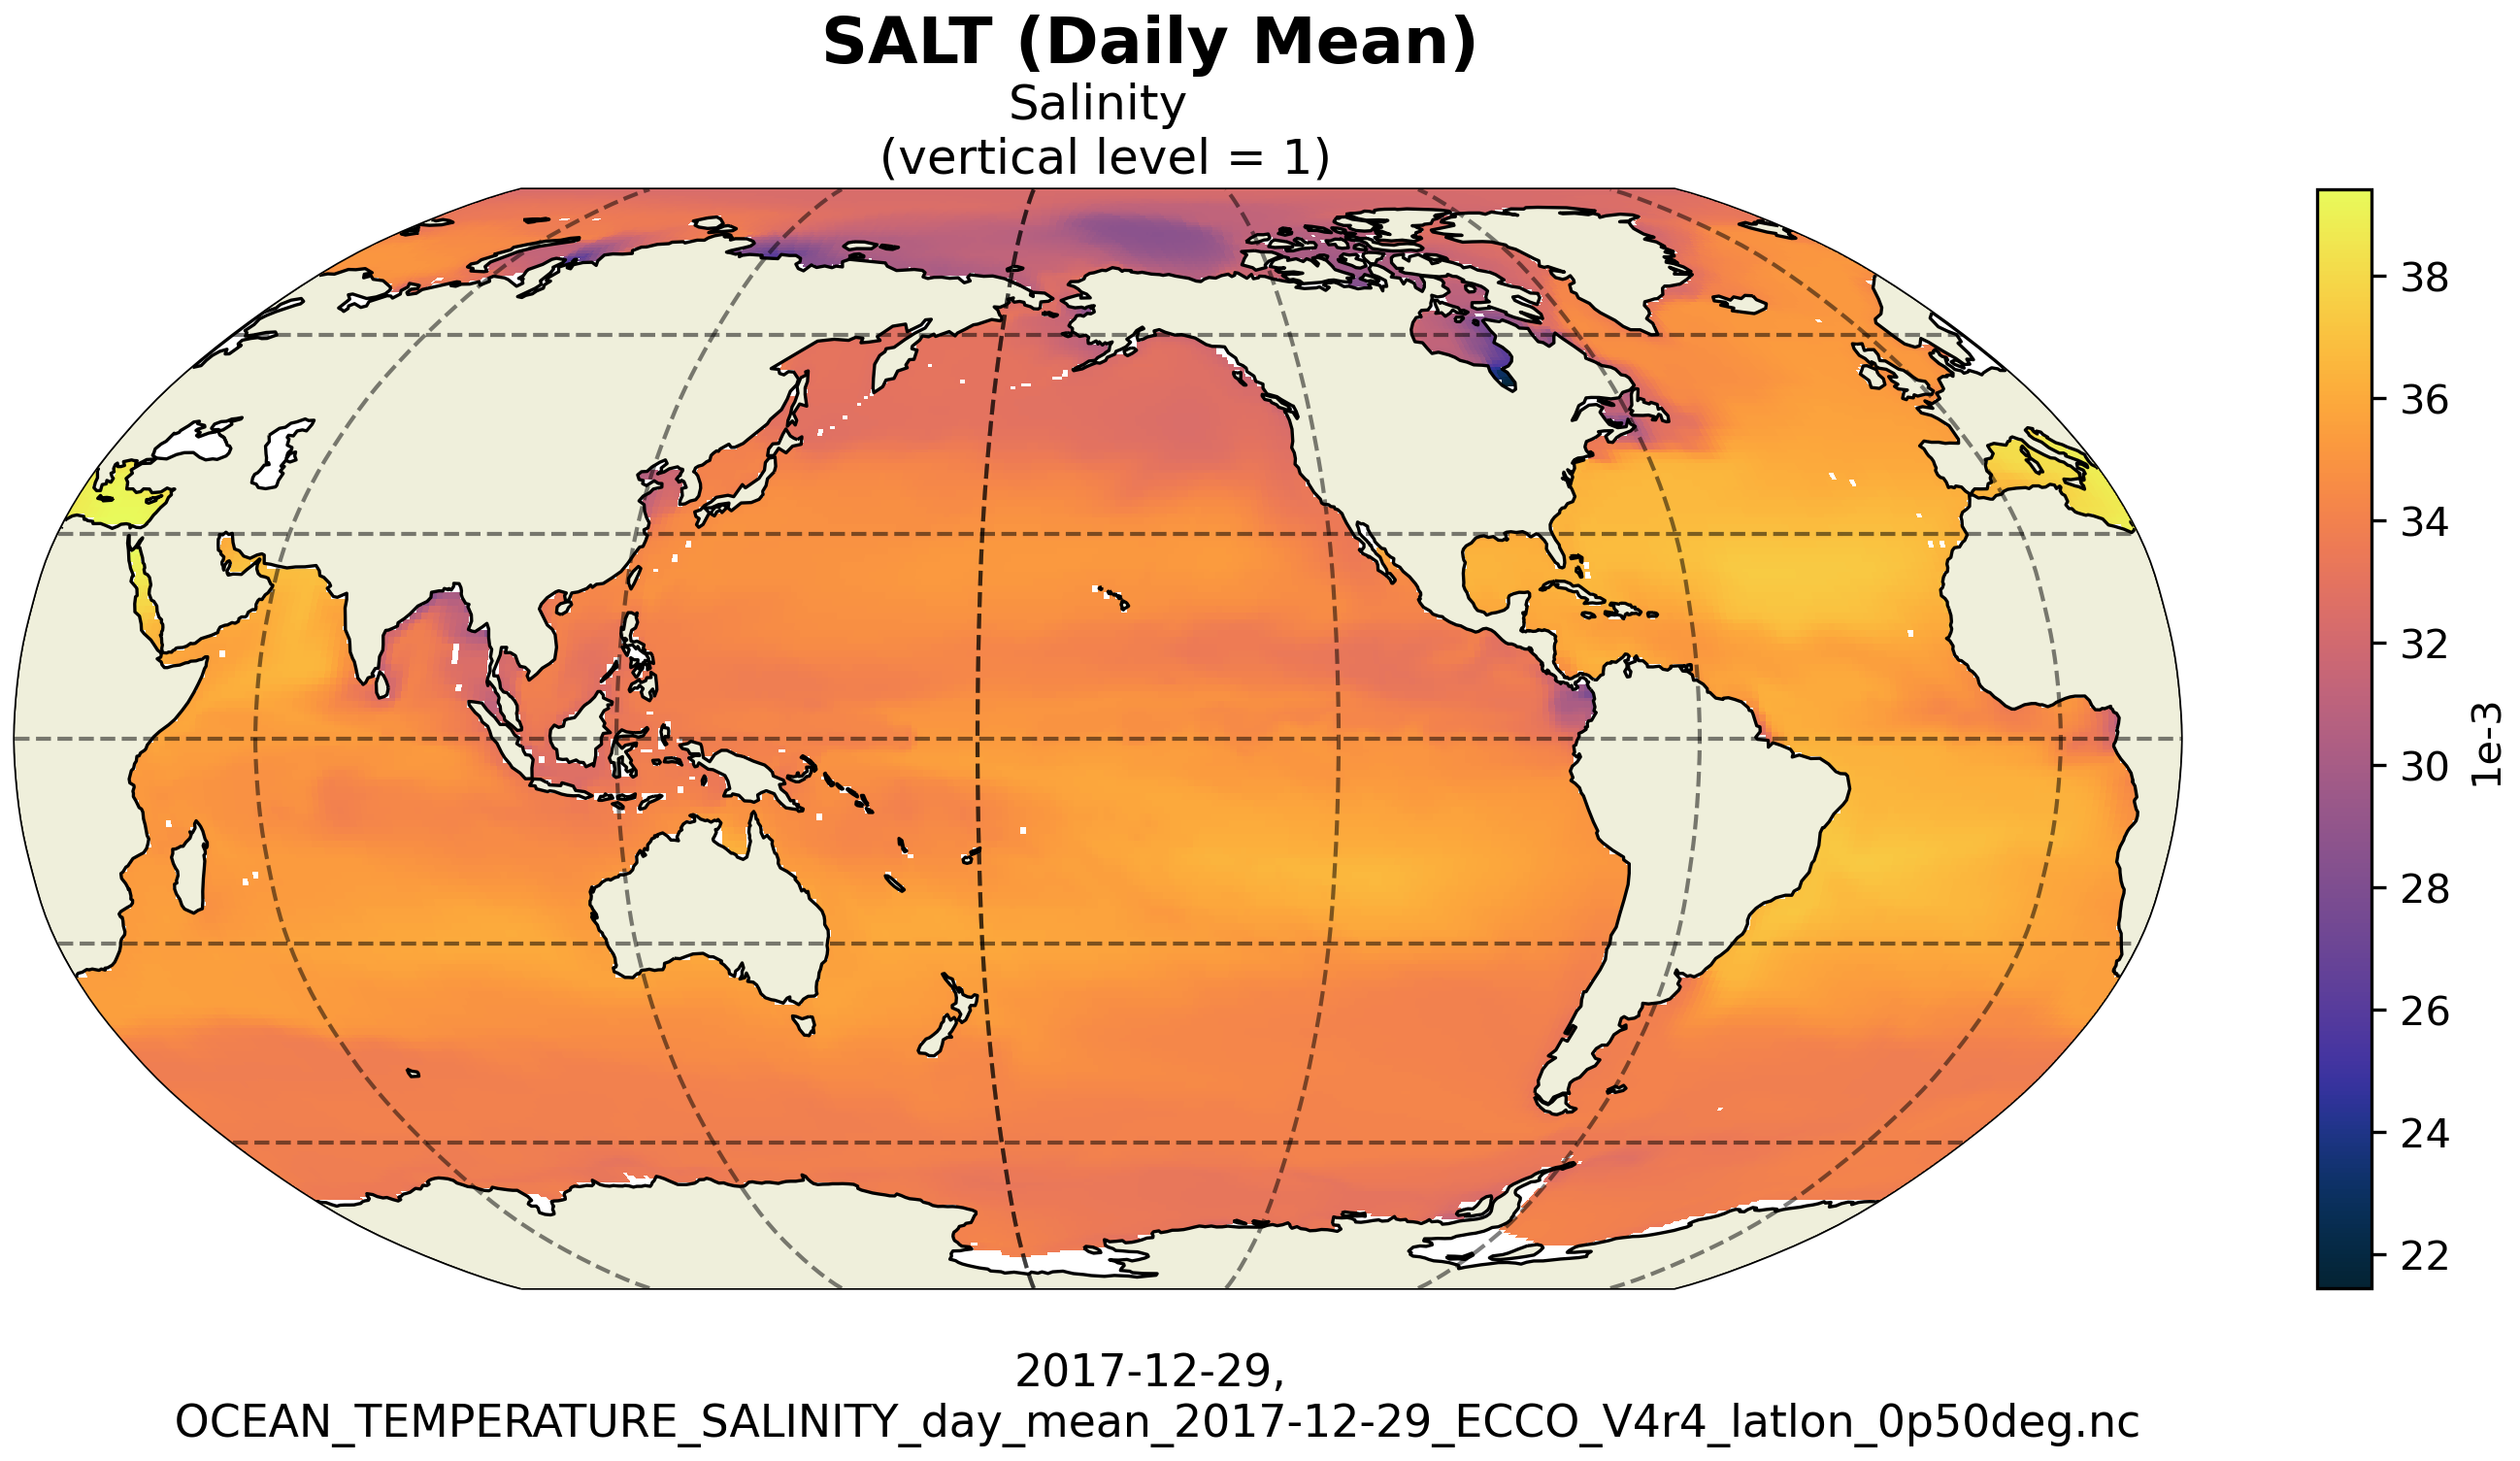
\includegraphics[width=\textwidth]{../images/plots/latlon_plots/Ocean_Temperature_and_Salinity/SALT.png}
\caption{Dataset: OCEAN\_TEMPERATURE\_SALINITY Variable: SALT}
\label{tab:table-OCEAN_TEMPERATURE_SALINITY_SALT-Plot}
\end{figure}
\pagebreak
\subsubsection{Latlon Variable THETA}
\begin{longtable}{|p{0.06\textwidth}|p{0.41\textwidth}|p{0.39\textwidth}|p{0.06\textwidth}|}
\caption{CDL description of OCEAN\_TEMPERATURE\_SALINITY's THETA variable}
\label{tab:table-OCEAN_TEMPERATURE_SALINITY_THETA} \\ 
\hline \endhead \hline \endfoot
\rowcolor{lightgray} \textbf{Storage Type} & \textbf{Variable Name} & \textbf{Description} & \textbf{Unit} \\ \hline
float32 & THETA & Potential temperature  & degree\_C \\ \hline
\rowcolor{lightgray}  \multicolumn{4}{|p{1.00\textwidth}|}{\textbf{CDL Description}} \\ \hline
\multicolumn{4}{|p{1.00\textwidth}|}{\makecell{\parbox{1\textwidth}{float32 THETA(time, Z, latitude, longitude)\\
\hspace*{0.5cm}THETA: \_FillValue = 9.96921e+36\\
\hspace*{0.5cm}THETA: coverage\_content\_type = modelResult\\
\hspace*{0.5cm}THETA: long\_name = Potential temperature \\
\hspace*{0.5cm}THETA: standard\_name = sea\_water\_potential\_temperature\\
\hspace*{0.5cm}THETA: units = degree\_C\\
\hspace*{0.5cm}THETA: coordinates = time Z\\
\hspace*{0.5cm}THETA: valid\_min = : 2.9179372787475586\\
\hspace*{0.5cm}THETA: valid\_max = 36.425140380859375}}} \\ \hline
\rowcolor{lightgray} \multicolumn{4}{|p{1.00\textwidth}|}{\textbf{Comments}} \\ \hline
\multicolumn{4}{|p{1\textwidth}|}{Sea water potential temperature is the temperature a parcel of sea water would have if moved adiabatically to sea level pressure. Note: the equation of state is a modified UNESCO formula by Jackett and McDougall (1995), which uses the model variable potential temperature as input assuming a horizontally and temporally constant pressure of \$p\_0=-g 
ho\_\{0\} z\$.} \\ \hline
\end{longtable}

\begin{figure}[H]
\centering
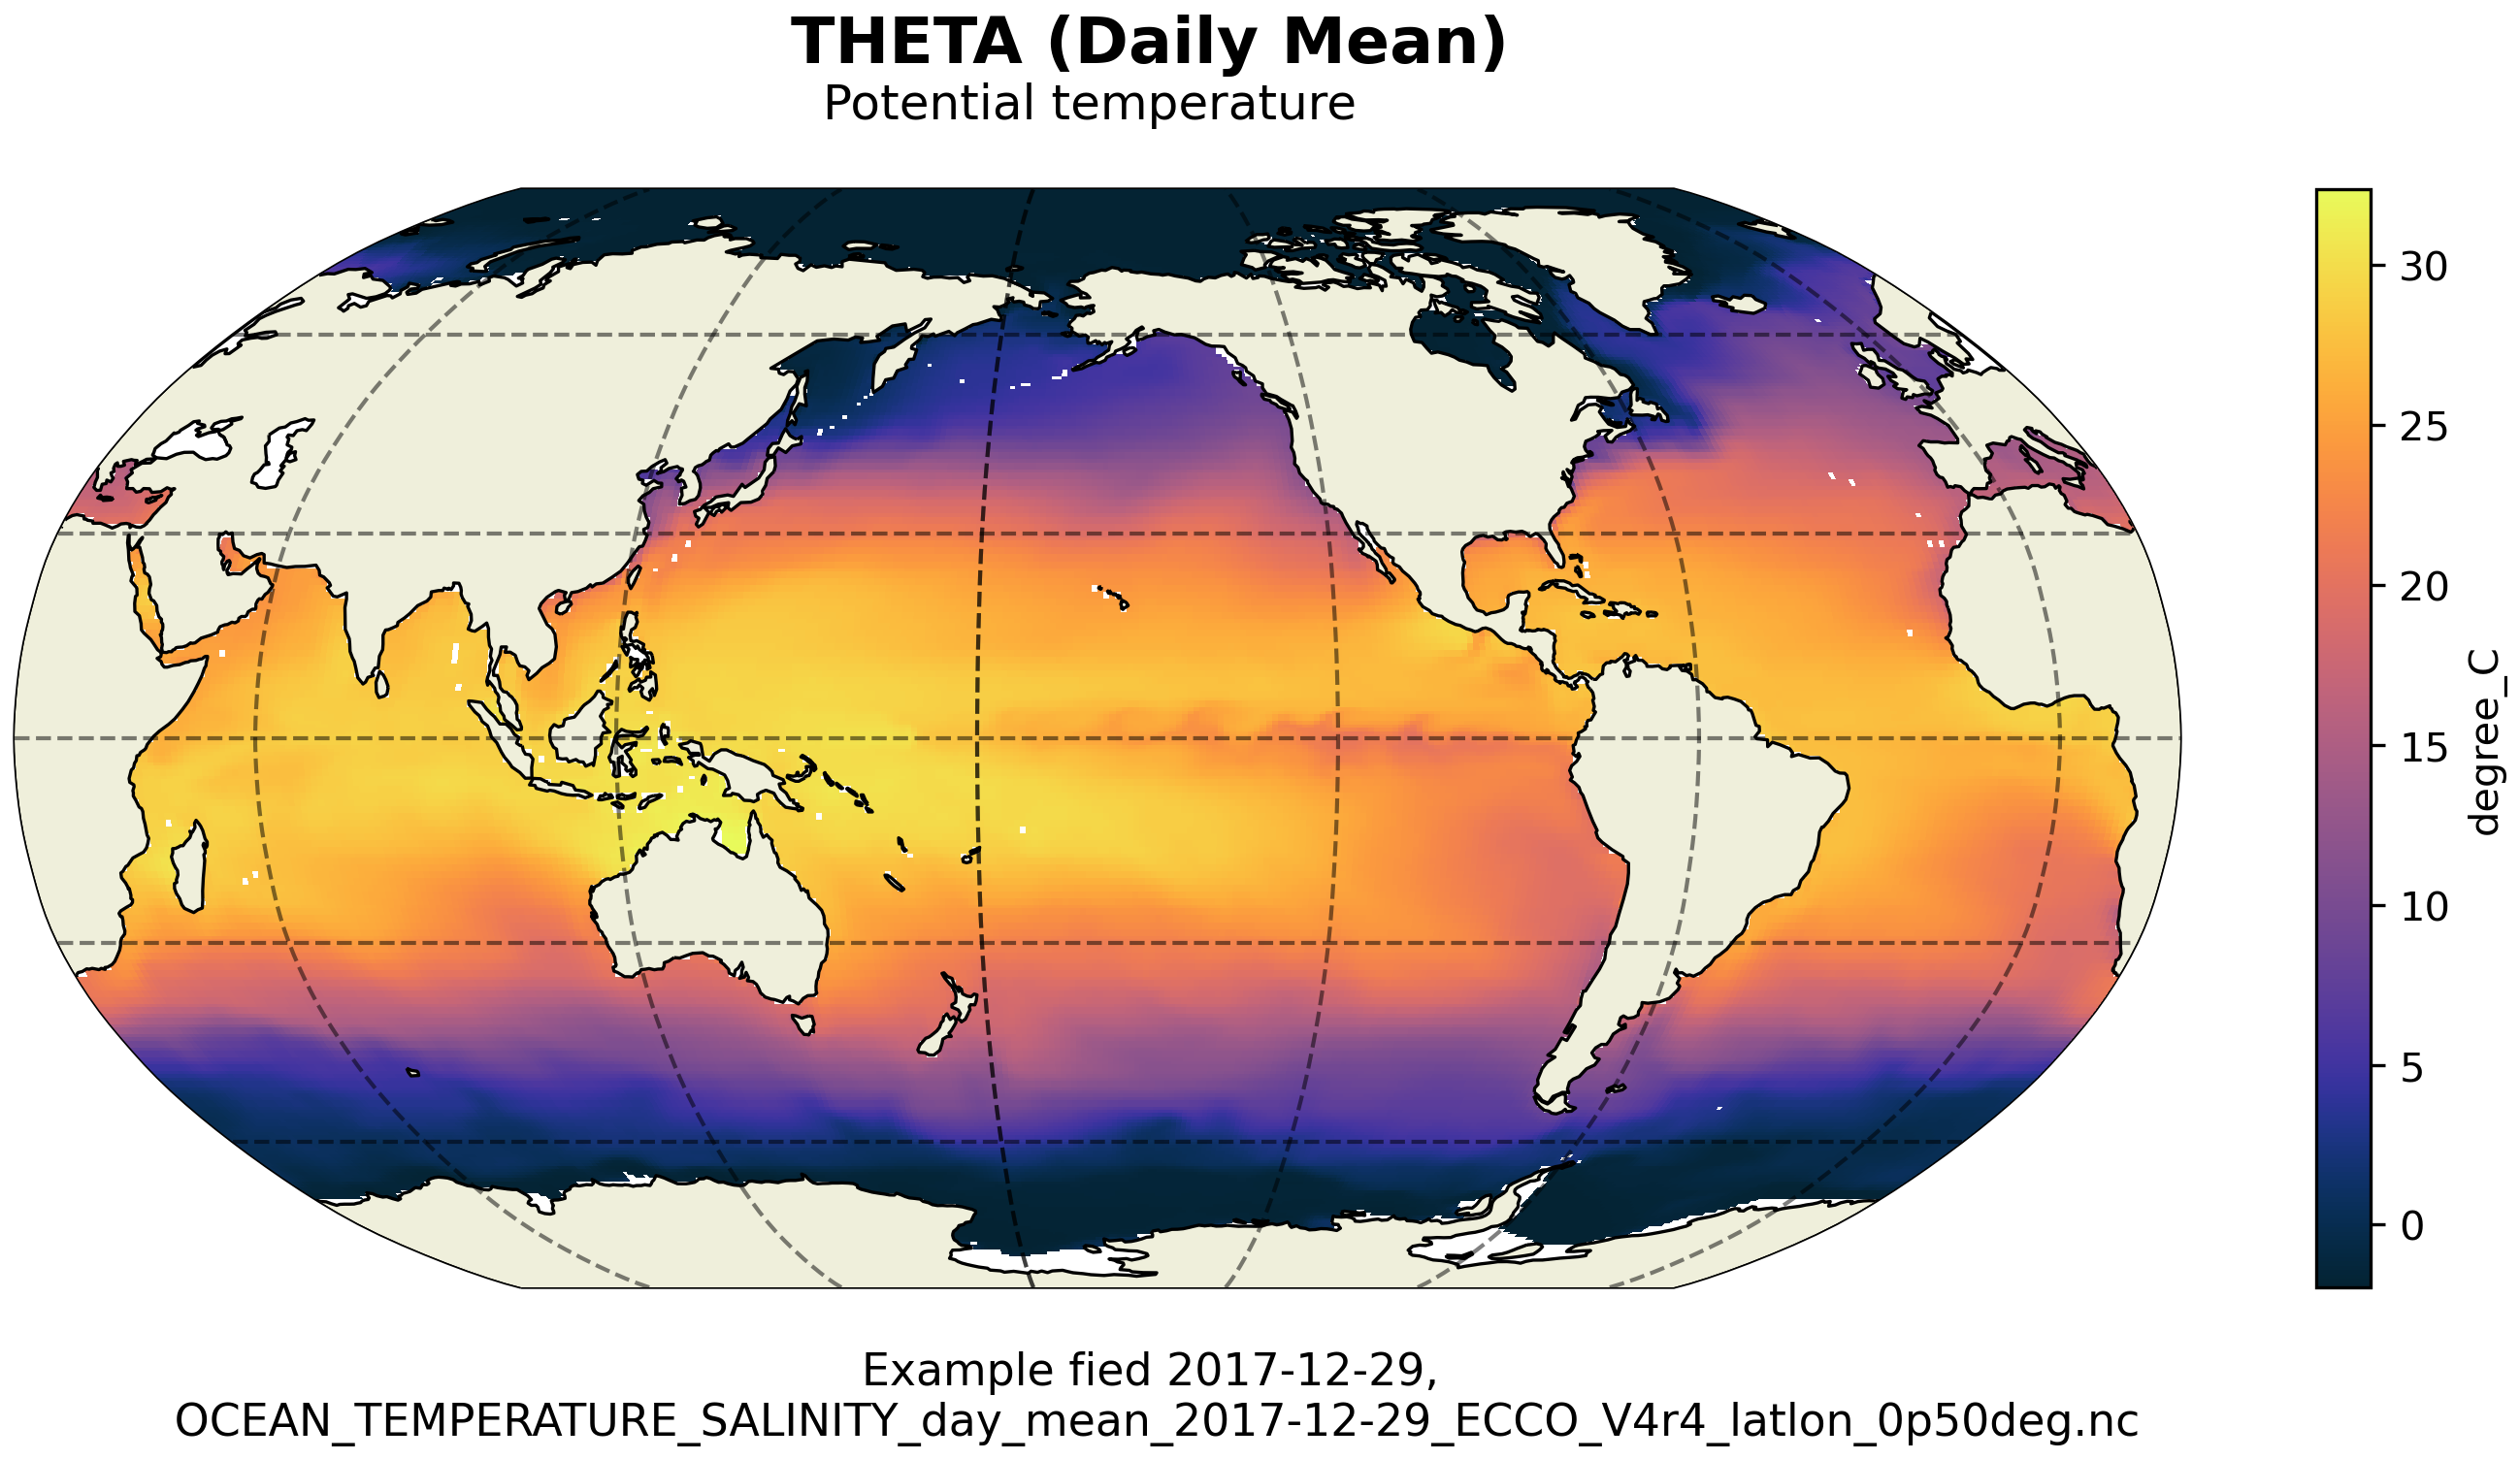
\includegraphics[width=\textwidth]{../images/plots/latlon_plots/Ocean_Temperature_and_Salinity/THETA.png}
\caption{Dataset: OCEAN\_TEMPERATURE\_SALINITY Variable: THETA}
\label{tab:table-OCEAN_TEMPERATURE_SALINITY_THETA-Plot}
\end{figure}
\pagebreak
\subsection{Latlon NetCDF OCEAN\_VELOCITY}
\newp
\begin{longtable}{|p{0.1\textwidth}|p{0.5\textwidth}|}
\caption{Variables in the dataset OCEAN\_VELOCITY}
\label{tab:table-OCEAN_VELOCITY-fields} \\ 
\hline \endhead \hline \endfoot
\rowcolor{lightgray} \textbf{Dataset:} & \textbf{OCEAN\_VELOCITY} \\ \hline
Field: &EVEL \\ \hline
Field: &NVEL \\ \hline
Field: &WVEL \\ \hline
\end{longtable}

\pagebreak
\subsubsection{Latlon Variable EVEL}
\begin{longtable}{|p{0.06\textwidth}|p{0.41\textwidth}|p{0.39\textwidth}|p{0.06\textwidth}|}
\caption{CDL description of OCEAN\_VELOCITY's EVEL variable}
\label{tab:table-OCEAN_VELOCITY_EVEL} \\ 
\hline \endhead \hline \endfoot
\rowcolor{lightgray} \textbf{Storage Type} & \textbf{Variable Name} & \textbf{Description} & \textbf{Unit} \\ \hline
float32 & EVEL & Zonal (east-west) velocity & m s-1 \\ \hline
\rowcolor{lightgray}  \multicolumn{4}{|p{1.00\textwidth}|}{\textbf{CDL Description}} \\ \hline
\multicolumn{4}{|p{1.00\textwidth}|}{\makecell{\parbox{1\textwidth}{float32 EVEL(time, Z, latitude, longitude)\\
\hspace*{0.5cm}EVEL: \_FillValue = 9.96921e+36\\
\hspace*{0.5cm}EVEL: coverage\_content\_type = modelResult\\
\hspace*{0.5cm}EVEL: long\_name = Zonal (east: west) velocity\\
\hspace*{0.5cm}EVEL: standard\_name = eastward\_sea\_water\_velocity\\
\hspace*{0.5cm}EVEL: units = m s: 1\\
\hspace*{0.5cm}EVEL: coordinates = Z time\\
\hspace*{0.5cm}EVEL: valid\_min = : 1.746832251548767\\
\hspace*{0.5cm}EVEL: valid\_max = 1.948591947555542}}} \\ \hline
\rowcolor{lightgray} \multicolumn{4}{|p{1.00\textwidth}|}{\textbf{Comments}} \\ \hline
\multicolumn{4}{|p{1\textwidth}|}{Zonal (east-west) component of ocean velocity. Note: EVEL is calculated by interpolating the model's x and y components of ocean velocity (UVEL and VVEL)to tracer cell centers and then finding the zonal component of the interpolated vectors. It is not recommended to use EVEL and NVEL for volume budget calculations because interpolating UVEL and VVEL from the model grid to the lat-lon grid introduces errors. Perform volume budget calculations with UVELMASS and VVELMASS on the native model grid.} \\ \hline
\end{longtable}

\begin{figure}[H]
\centering
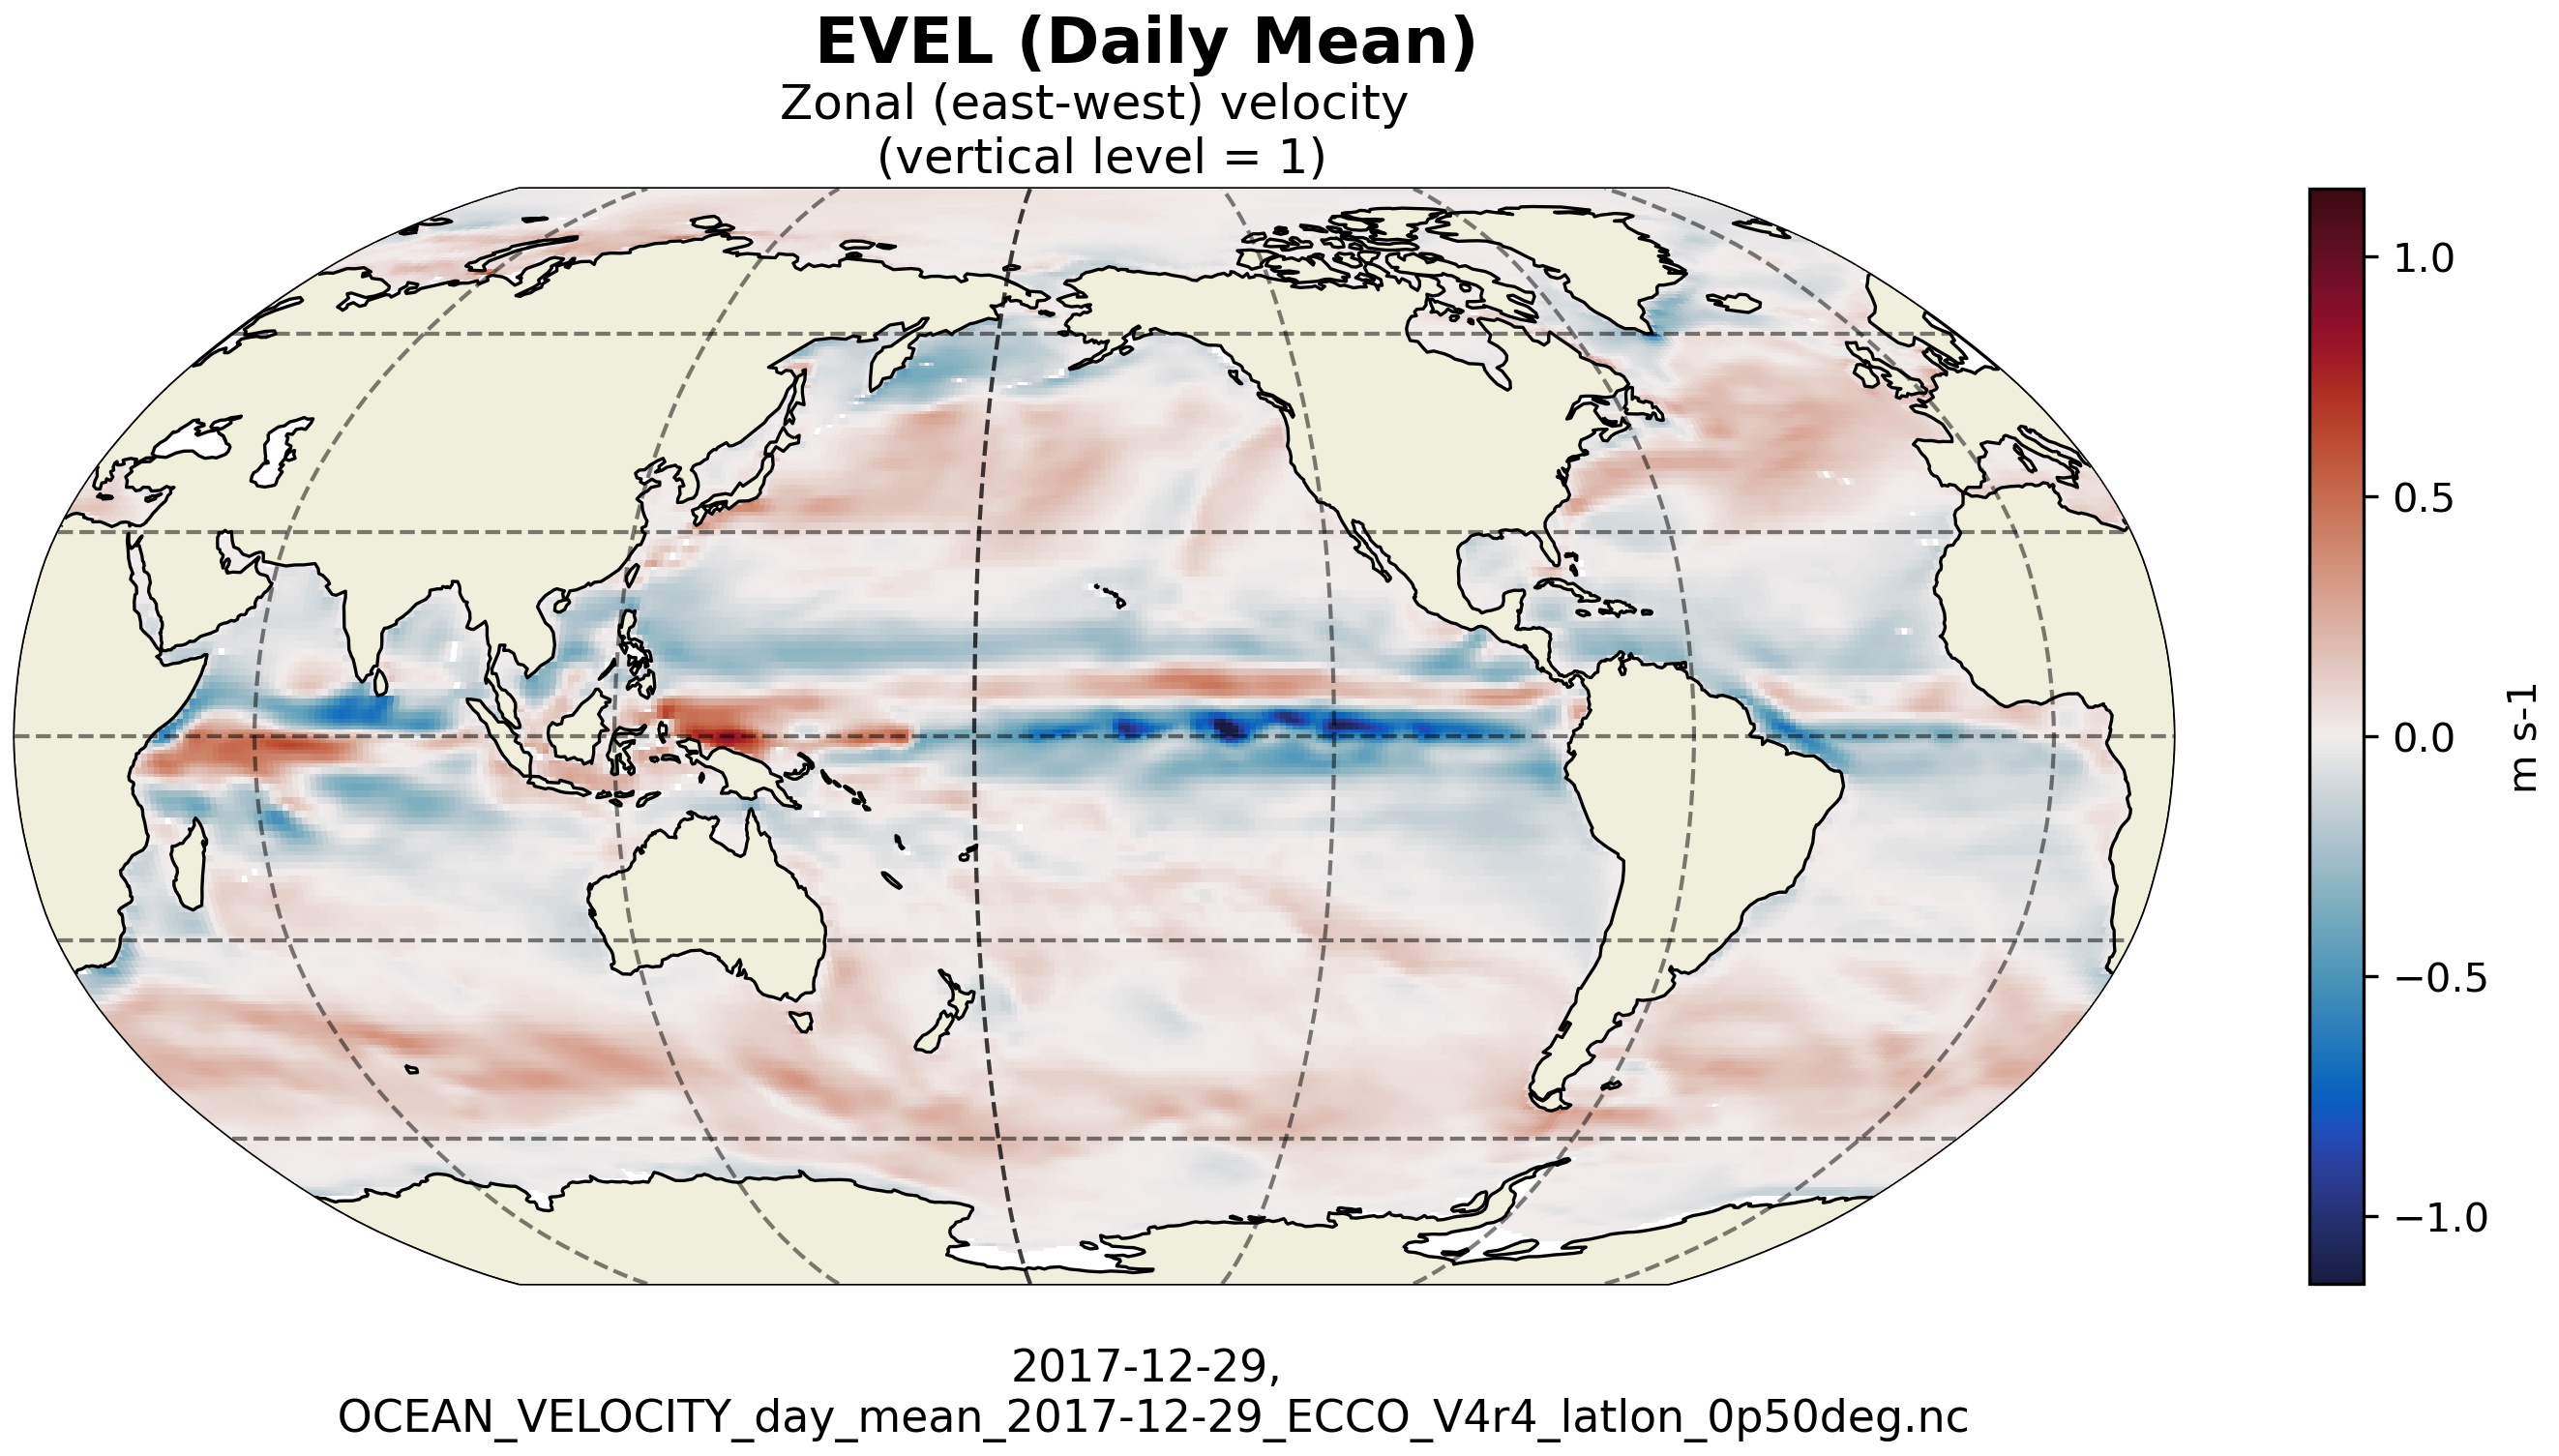
\includegraphics[width=\textwidth]{../images/plots/latlon_plots/Ocean_Velocity/EVEL.png}
\caption{Dataset: OCEAN\_VELOCITY Variable: EVEL}
\label{tab:table-OCEAN_VELOCITY_EVEL-Plot}
\end{figure}
\pagebreak
\subsubsection{Latlon Variable NVEL}
\begin{longtable}{|p{0.06\textwidth}|p{0.41\textwidth}|p{0.39\textwidth}|p{0.06\textwidth}|}
\caption{CDL description of OCEAN\_VELOCITY's NVEL variable}
\label{tab:table-OCEAN_VELOCITY_NVEL} \\ 
\hline \endhead \hline \endfoot
\rowcolor{lightgray} \textbf{Storage Type} & \textbf{Variable Name} & \textbf{Description} & \textbf{Unit} \\ \hline
float32 & NVEL & Meridional (north-south) velocity & m s-1 \\ \hline
\rowcolor{lightgray}  \multicolumn{4}{|p{1.00\textwidth}|}{\textbf{CDL Description}} \\ \hline
\multicolumn{4}{|p{1.00\textwidth}|}{\makecell{\parbox{1\textwidth}{float32 NVEL(time, Z, latitude, longitude)\\
\hspace*{0.5cm}NVEL: \_FillValue = 9.96921e+36\\
\hspace*{0.5cm}NVEL: coverage\_content\_type = modelResult\\
\hspace*{0.5cm}NVEL: long\_name = Meridional (north: south) velocity\\
\hspace*{0.5cm}NVEL: standard\_name = northward\_sea\_water\_velocity\\
\hspace*{0.5cm}NVEL: units = m s: 1\\
\hspace*{0.5cm}NVEL: coordinates = Z time\\
\hspace*{0.5cm}NVEL: valid\_min = : 1.2522369623184204\\
\hspace*{0.5cm}NVEL: valid\_max = 2.0500051975250244}}} \\ \hline
\rowcolor{lightgray} \multicolumn{4}{|p{1.00\textwidth}|}{\textbf{Comments}} \\ \hline
\multicolumn{4}{|p{1\textwidth}|}{Meridional (north-south) component of ocean velocity. Note: NVEL is calculated by interpolating the model's x and y components of ocean velocity (UVEL and VVEL) to tracer cell centers and then finding the meridional component of the interpolated vectors. It is not recommended to use EVEL and NVEL for volume budget calculations because interpolating UVEL and VVEL from the model grid to the lat-lon grid introduces errors. Perform volume budget calculations with UVELMASS and VVELMASS on the native model grid.} \\ \hline
\end{longtable}

\begin{figure}[H]
\centering
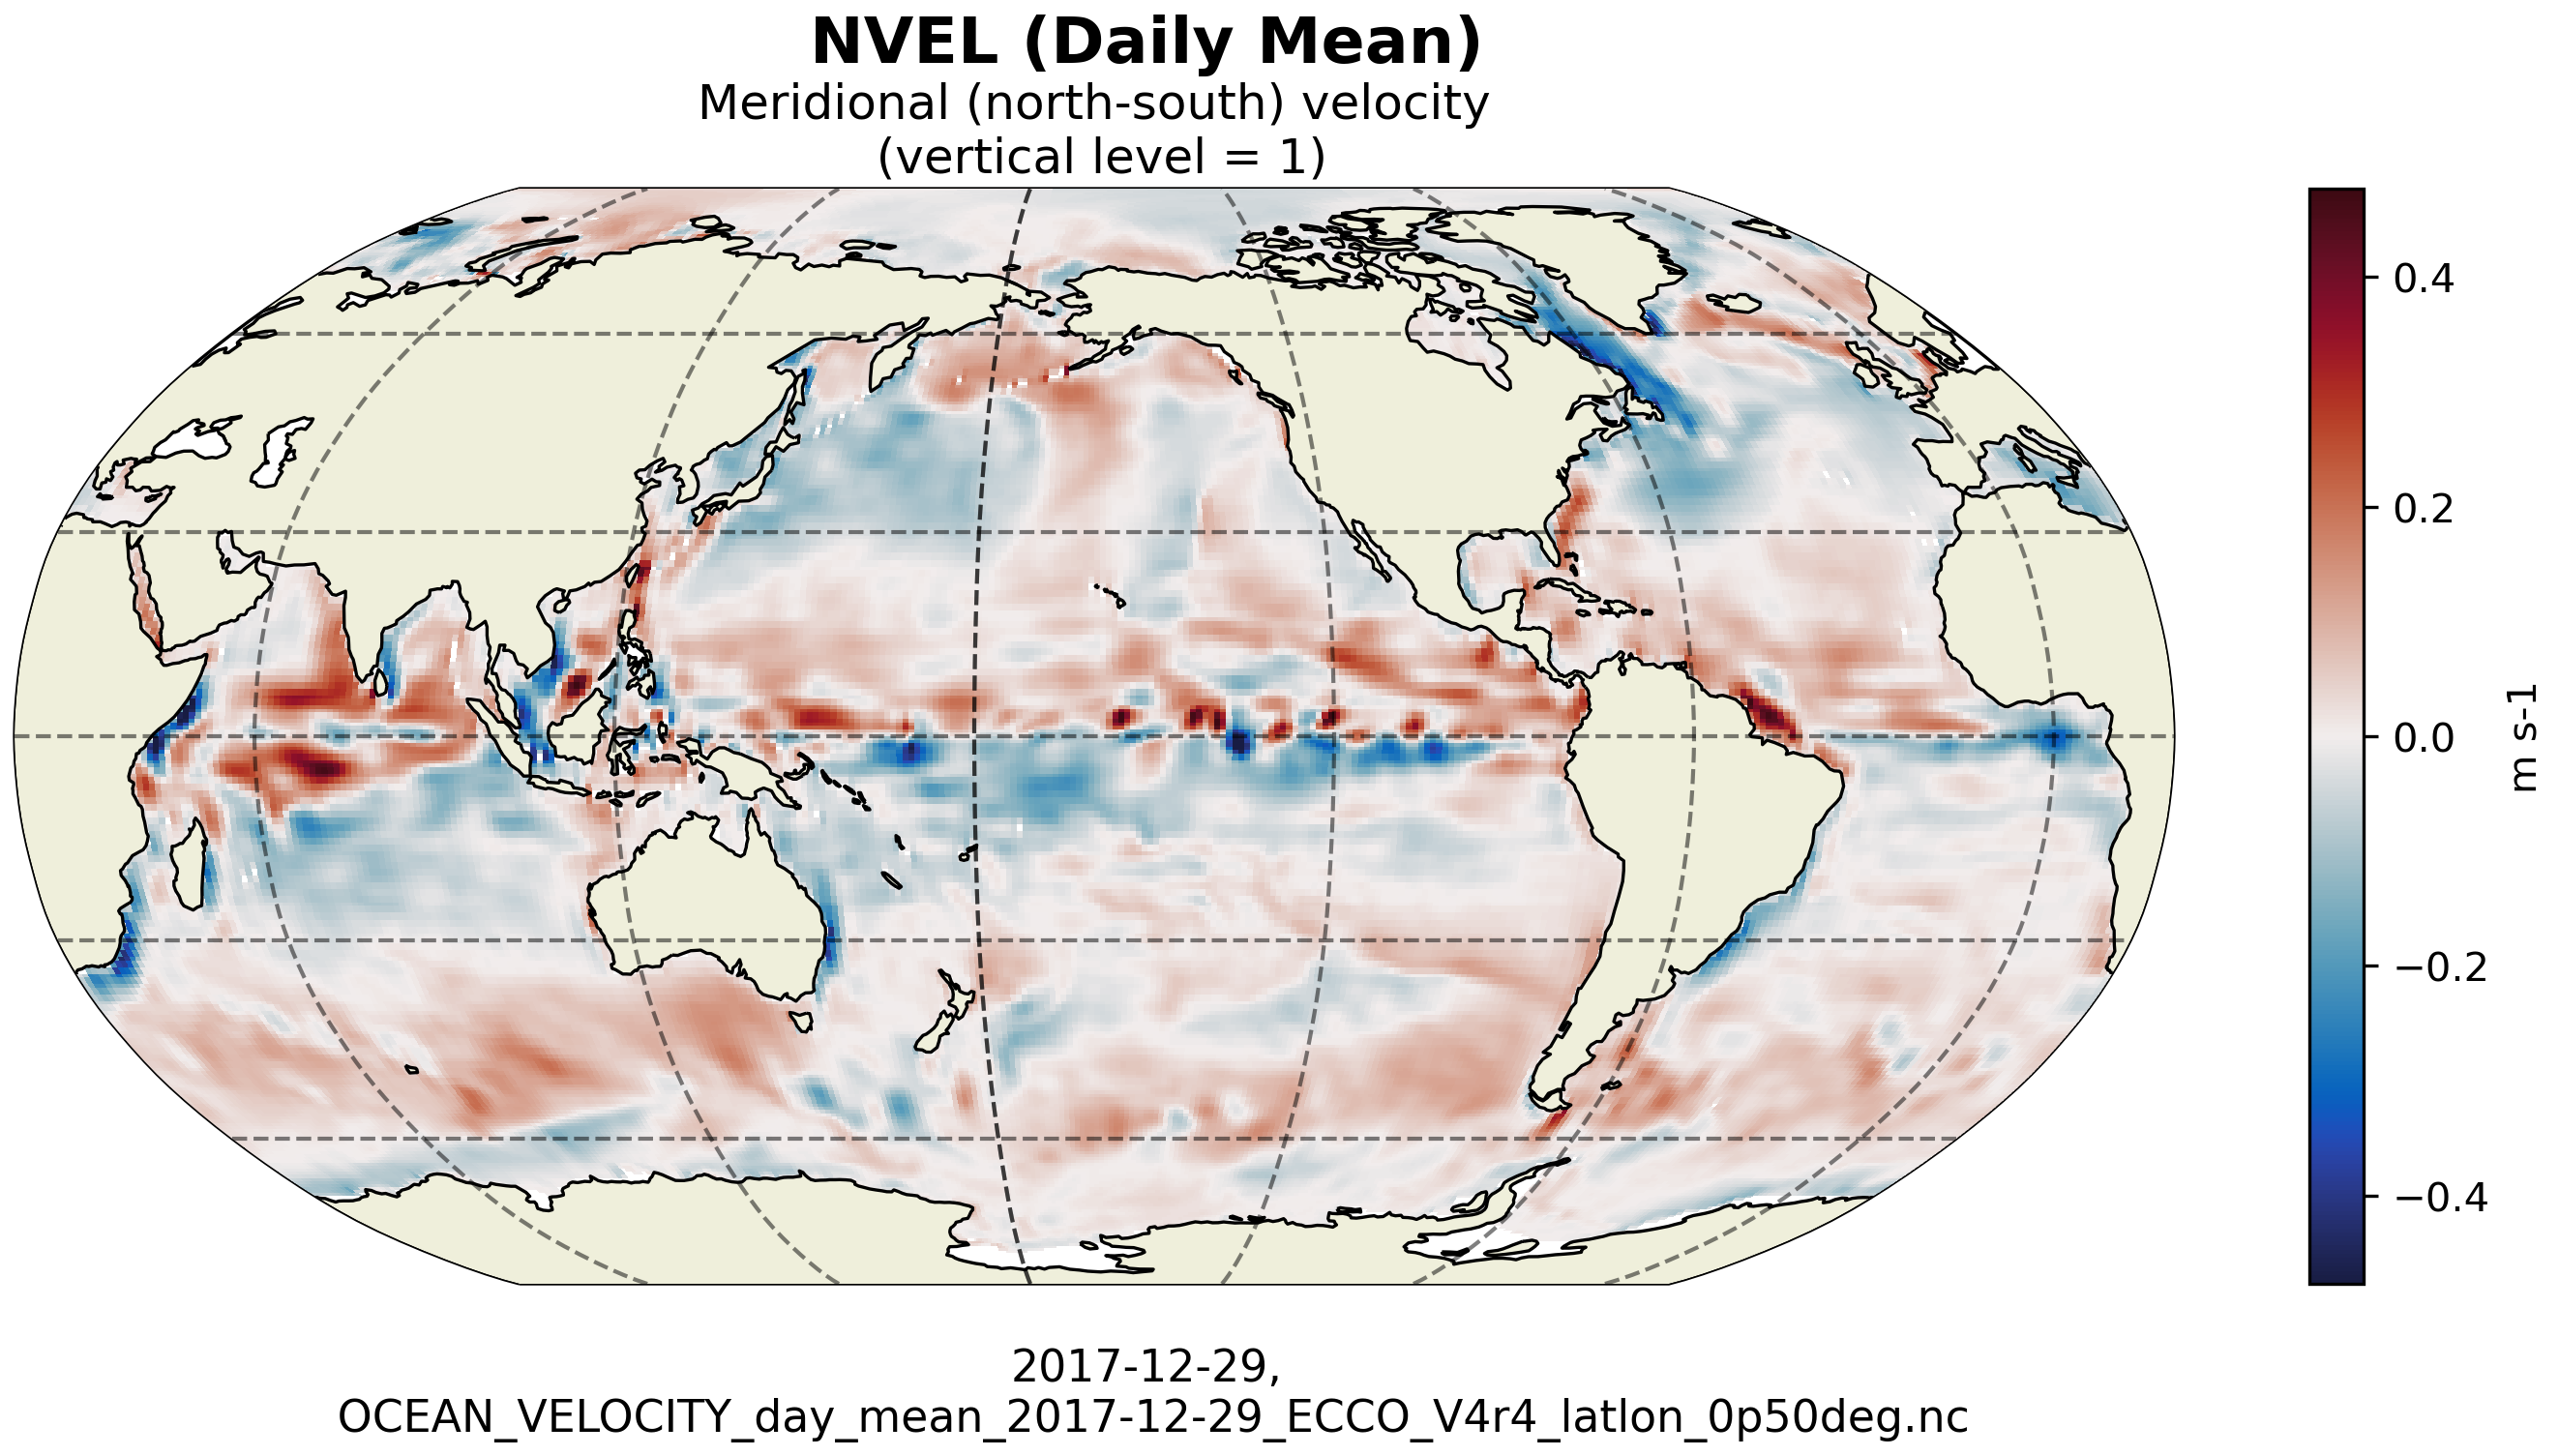
\includegraphics[width=\textwidth]{../images/plots/latlon_plots/Ocean_Velocity/NVEL.png}
\caption{Dataset: OCEAN\_VELOCITY Variable: NVEL}
\label{tab:table-OCEAN_VELOCITY_NVEL-Plot}
\end{figure}
\pagebreak
\subsubsection{Latlon Variable WVEL}
\begin{longtable}{|p{0.06\textwidth}|p{0.41\textwidth}|p{0.39\textwidth}|p{0.06\textwidth}|}
\caption{CDL description of OCEAN\_VELOCITY's WVEL variable}
\label{tab:table-OCEAN_VELOCITY_WVEL} \\ 
\hline \endhead \hline \endfoot
\rowcolor{lightgray} \textbf{Storage Type} & \textbf{Variable Name} & \textbf{Description} & \textbf{Unit} \\ \hline
float32 & WVEL & Vertical velocity & m s-1 \\ \hline
\rowcolor{lightgray}  \multicolumn{4}{|p{1.00\textwidth}|}{\textbf{CDL Description}} \\ \hline
\multicolumn{4}{|p{1.00\textwidth}|}{\makecell{\parbox{1\textwidth}{float32 WVEL(time, Z, latitude, longitude)\\
\hspace*{0.5cm}WVEL: \_FillValue = 9.96921e+36\\
\hspace*{0.5cm}WVEL: coverage\_content\_type = modelResult\\
\hspace*{0.5cm}WVEL: direction = >0 decreases volume\\
\hspace*{0.5cm}WVEL: long\_name = Vertical velocity\\
\hspace*{0.5cm}WVEL: standard\_name = upward\_sea\_water\_velocity\\
\hspace*{0.5cm}WVEL: units = m s: 1\\
\hspace*{0.5cm}WVEL: coordinates = Z time\\
\hspace*{0.5cm}WVEL: valid\_min = : 0.0023150660563260317\\
\hspace*{0.5cm}WVEL: valid\_max = 0.0016380994347855449}}} \\ \hline
\rowcolor{lightgray} \multicolumn{4}{|p{1.00\textwidth}|}{\textbf{Comments}} \\ \hline
\multicolumn{4}{|p{1\textwidth}|}{Vertical velocity in the +z direction at the top face of the grid cell. Note: in the Arakawa-C grid used in ECCO V4r4, vertical velocities are staggered relative to the tracer cell centers with values at the TOP and BOTTOM faces of each grid cell.} \\ \hline
\end{longtable}

\begin{figure}[H]
\centering
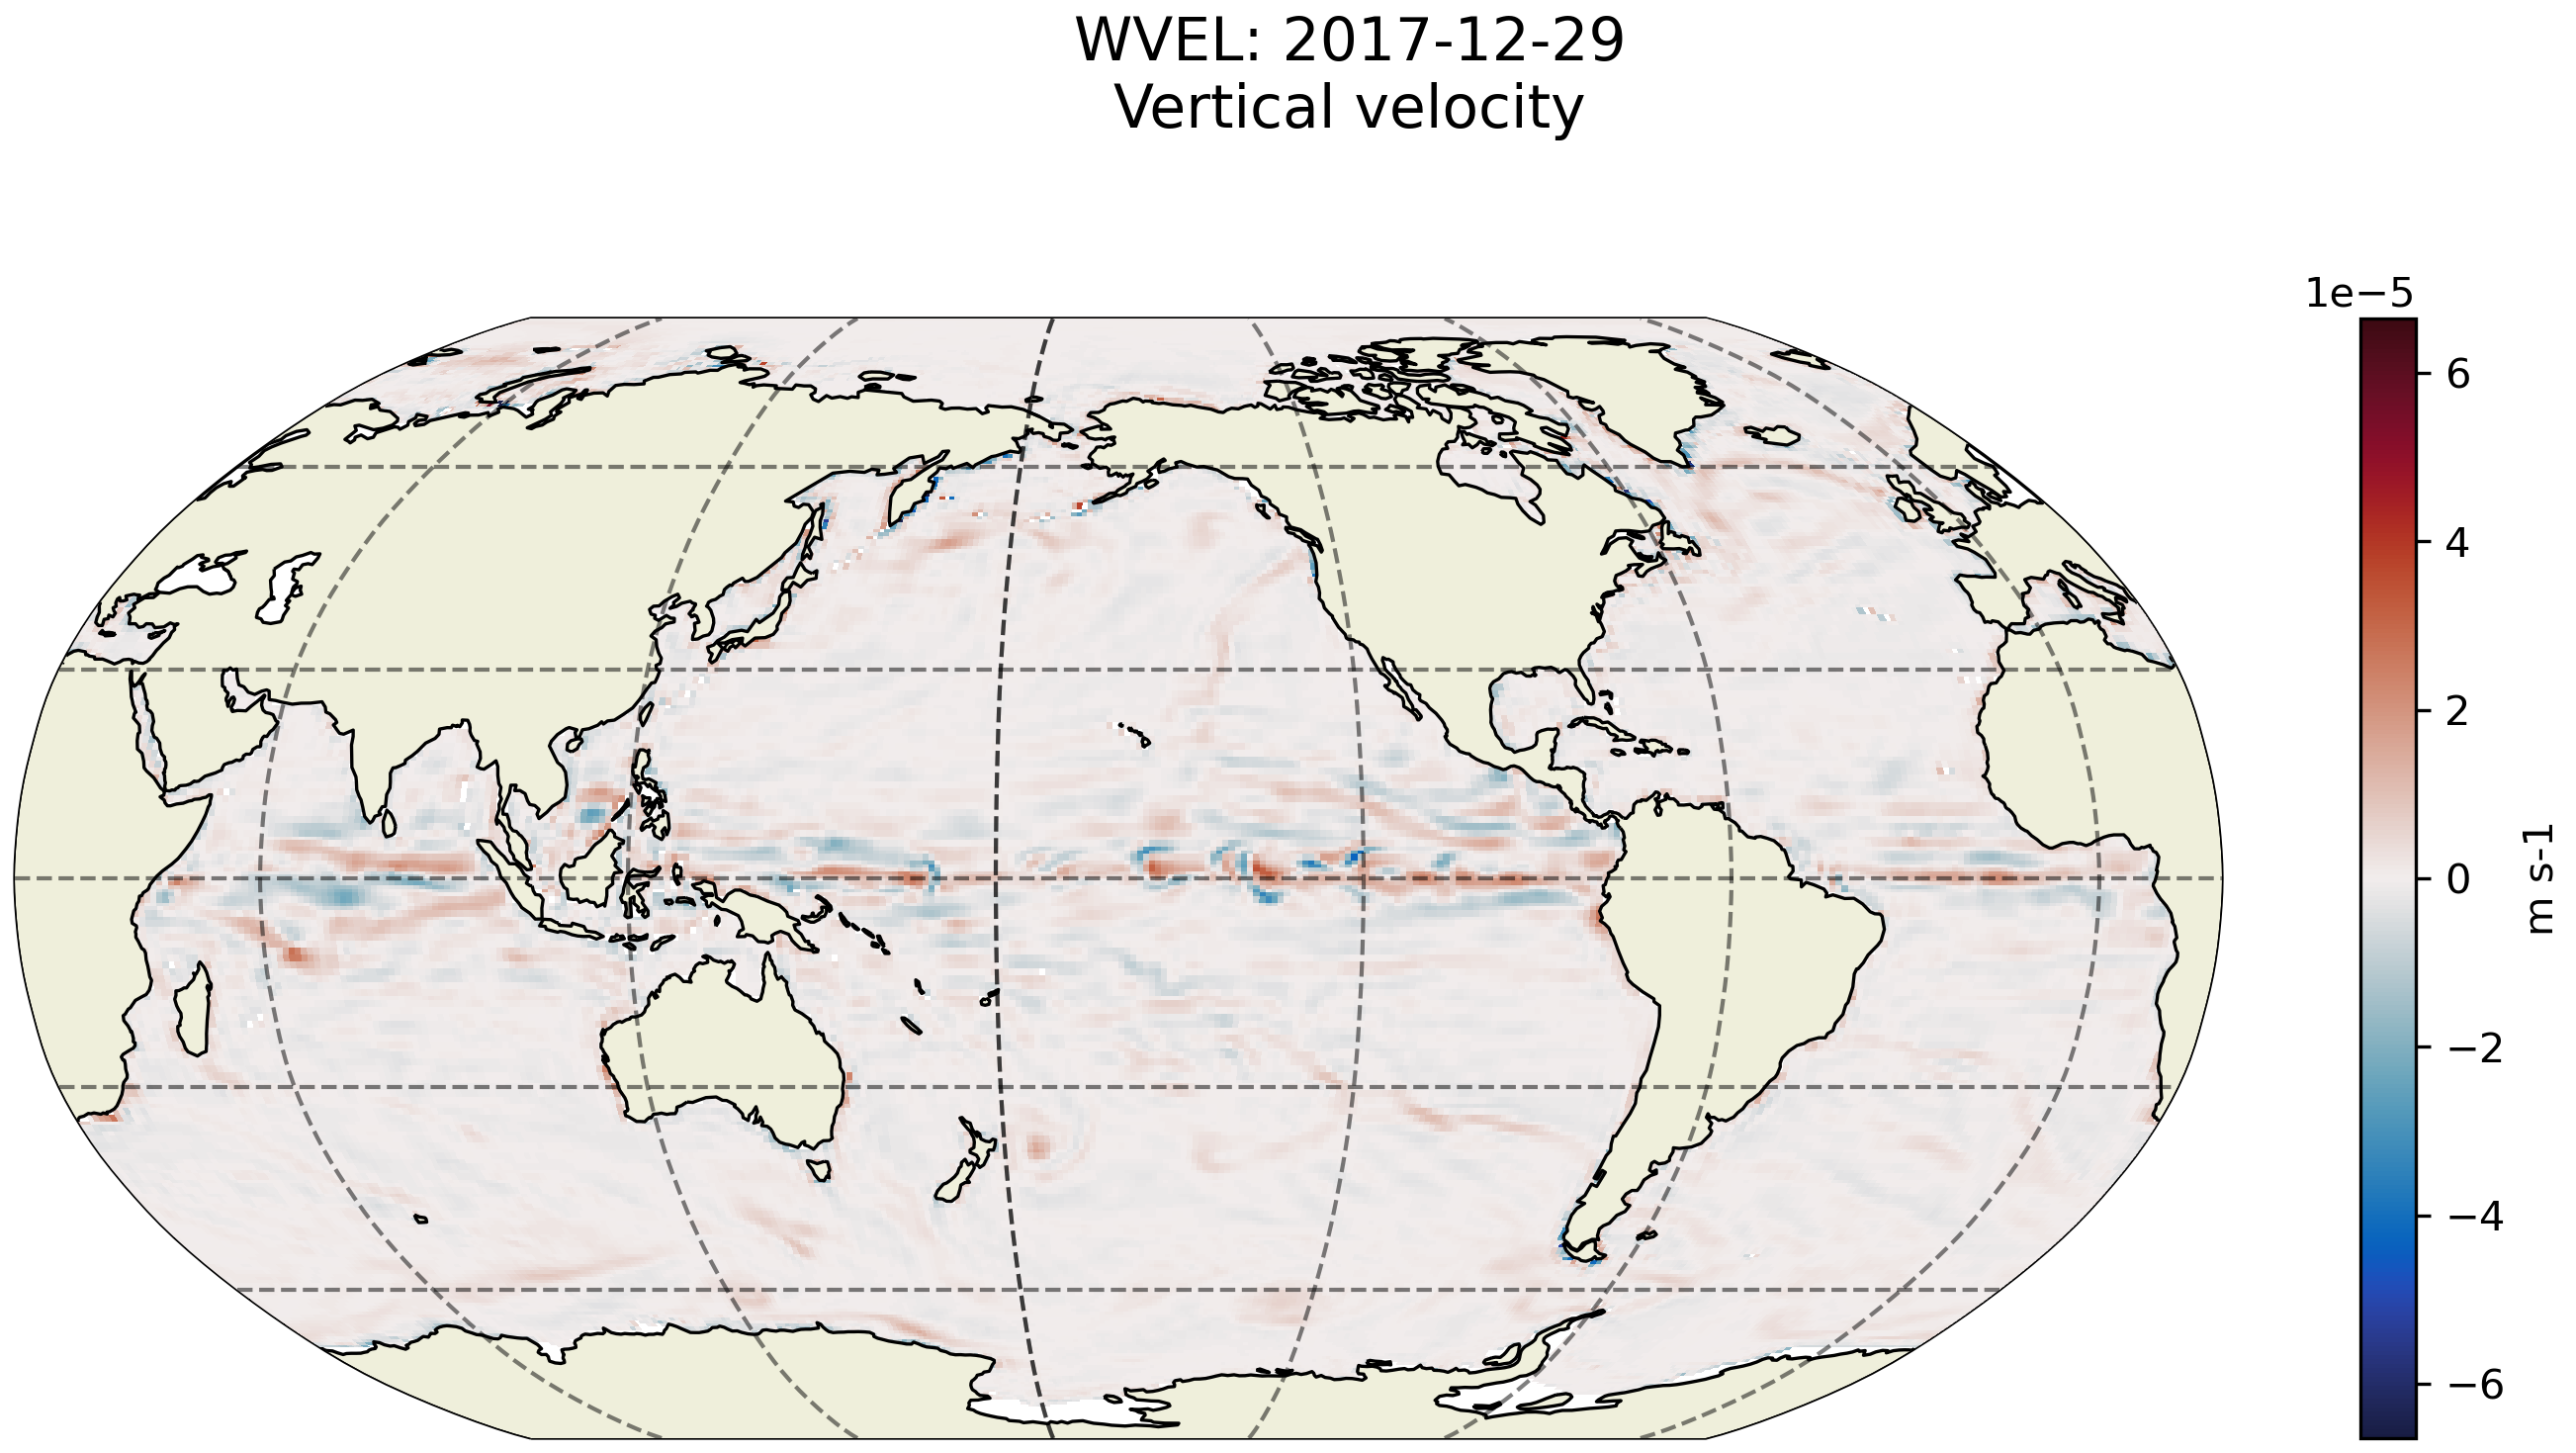
\includegraphics[width=\textwidth]{../images/plots/latlon_plots/Ocean_Velocity/WVEL.png}
\caption{Dataset: OCEAN\_VELOCITY Variable: WVEL}
\label{tab:table-OCEAN_VELOCITY_WVEL-Plot}
\end{figure}
\pagebreak
\subsection{Latlon NetCDF SEA\_ICE\_CONC\_THICKNESS}
\newp
\begin{longtable}{|p{0.1\textwidth}|p{0.5\textwidth}|}
\caption{Variables in the dataset SEA\_ICE\_CONC\_THICKNESS}
\label{tab:table-SEA_ICE_CONC_THICKNESS-fields} \\ 
\hline \endhead \hline \endfoot
\rowcolor{lightgray} \textbf{Dataset:} & \textbf{SEA\_ICE\_CONC\_THICKNESS} \\ \hline
Field: &SIarea \\ \hline
Field: &SIheff \\ \hline
Field: &SIhsnow \\ \hline
Field: &sIceLoad \\ \hline
\end{longtable}

\pagebreak
\subsubsection{Latlon Variable SIarea}
\begin{longtable}{|p{0.06\textwidth}|p{0.41\textwidth}|p{0.39\textwidth}|p{0.06\textwidth}|}
\caption{CDL description of SEA\_ICE\_CONC\_THICKNESS's SIarea variable}
\label{tab:table-SEA_ICE_CONC_THICKNESS_SIarea} \\ 
\hline \endhead \hline \endfoot
\rowcolor{lightgray} \textbf{Storage Type} & \textbf{Variable Name} & \textbf{Description} & \textbf{Unit} \\ \hline
float32 & SIarea & Sea-ice concentration & 1 \\ \hline
\rowcolor{lightgray}  \multicolumn{4}{|p{1.00\textwidth}|}{\textbf{CDL Description}} \\ \hline
\multicolumn{4}{|p{1.00\textwidth}|}{\makecell{\parbox{1\textwidth}{float32 SIarea(time, latitude, longitude)\\
\hspace*{0.5cm}SIarea: \_FillValue = 9.96921e+36\\
\hspace*{0.5cm}SIarea: coverage\_content\_type = modelResult\\
\hspace*{0.5cm}SIarea: long\_name = Sea: ice concentration\\
\hspace*{0.5cm}SIarea: standard\_name = sea\_ice\_area\_fraction\\
\hspace*{0.5cm}SIarea: units = 1\\
\hspace*{0.5cm}SIarea: coordinates = time\\
\hspace*{0.5cm}SIarea: valid\_min = 0.0\\
\hspace*{0.5cm}SIarea: valid\_max = 0.9700000286102295}}} \\ \hline
\rowcolor{lightgray} \multicolumn{4}{|p{1.00\textwidth}|}{\textbf{Comments}} \\ \hline
\multicolumn{4}{|p{1\textwidth}|}{Fraction of ocean grid cell covered with sea-ice [0 to 1]. CF Standard Name Table v73:  'Area fraction' is the fraction of a grid cell's horizontal area that has some characteristic of interest. It is evaluated as the area of interest divided by the grid cell area. It may be expressed as a fraction, a percentage, or any other dimensionless representation of a fraction. Sea ice area fraction is area of the sea surface occupied by sea ice. It is also called 'sea ice concentration'. 'Sea ice' means all ice floating in the sea which has formed from freezing sea water, rather than by other processes such as calving of land ice to form icebergs. https://cfconventions.org/Data/cf-standard-names/73/build/cf-standard-name-table.html. Defined using CF Standard Name Table v73: 'Area fraction' is the fraction of a grid cell's horizontal area that has some characteristic of interest. It is evaluated as the area of interest divided by the grid cell area. It may be expressed as a fraction, a percentage, or any other dimensionless representation of a fraction. Sea ice area fraction is area of the sea surface occupied by sea ice. It is also called 'sea ice concentration'. 'Sea ice' means all ice floating in the sea which has formed from freezing sea water and precipitation, rather than by other processes such as calving of land ice to form icebergs. https://cfconventions.org/Data/cf-standard-names/73/build/cf-standard-name-table.html} \\ \hline
\end{longtable}

\begin{figure}[H]
\centering
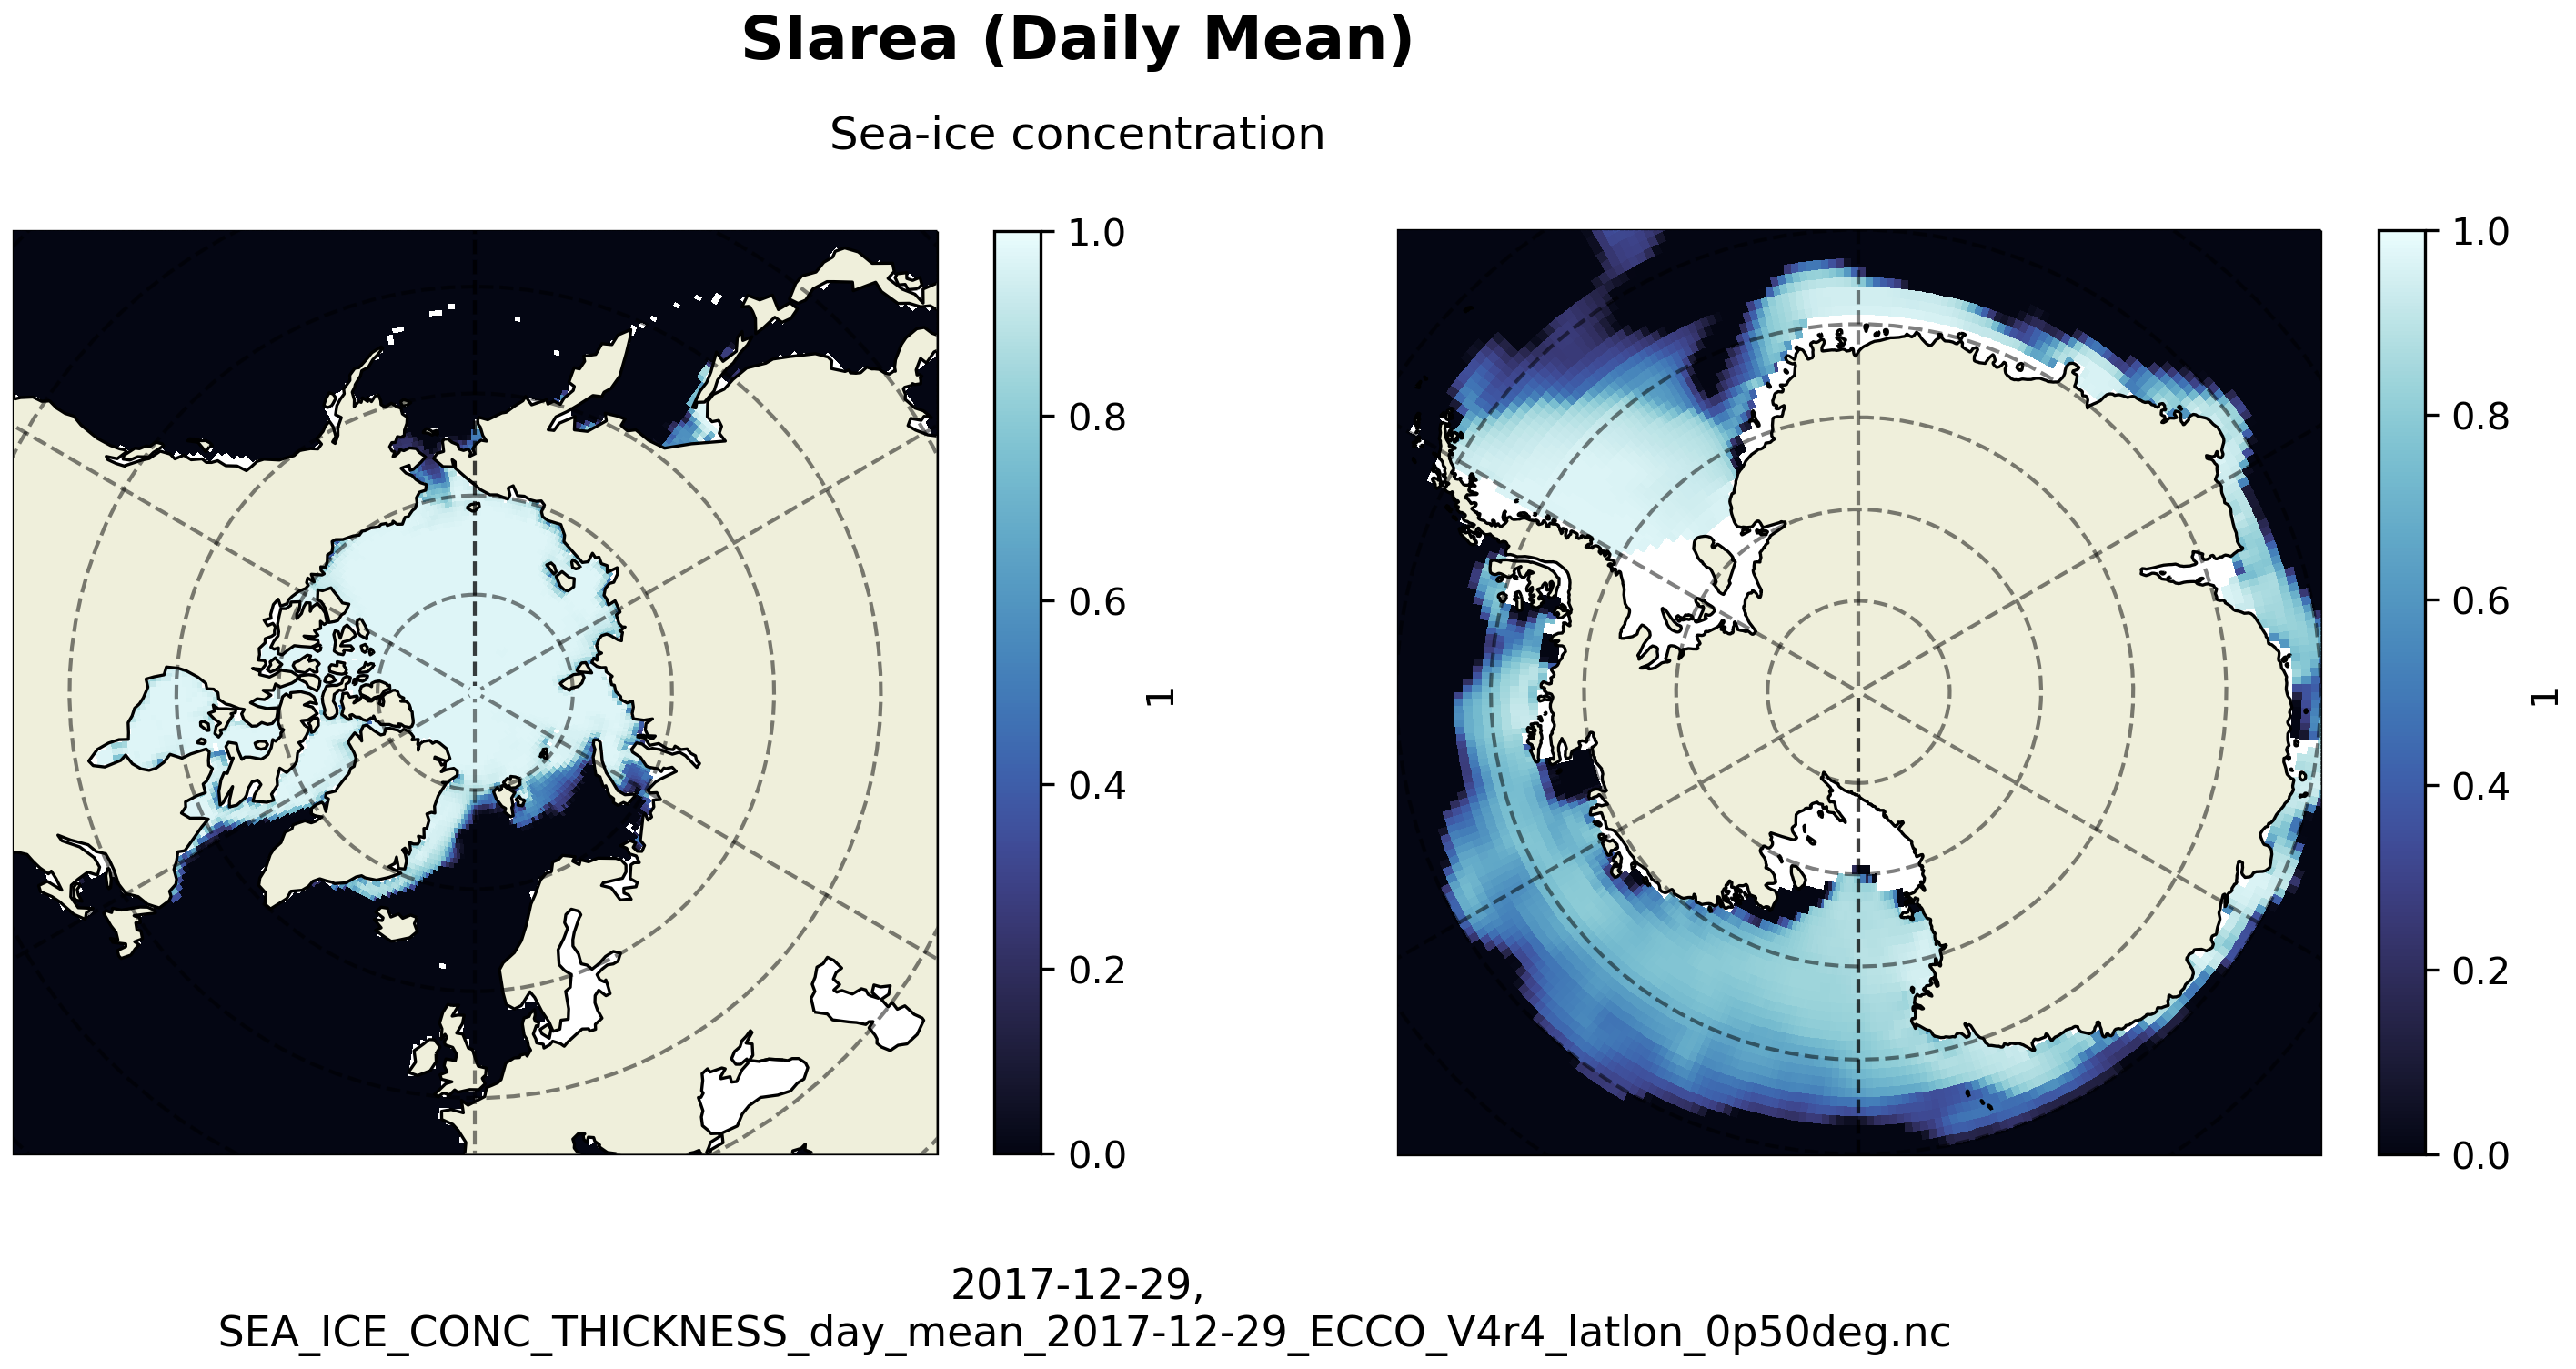
\includegraphics[width=\textwidth]{../images/plots/latlon_plots/Sea-Ice_and_Snow_Concentration_and_Thickness/SIarea.png}
\caption{Dataset: SEA\_ICE\_CONC\_THICKNESS Variable: SIarea}
\label{tab:table-SEA_ICE_CONC_THICKNESS_SIarea-Plot}
\end{figure}
\pagebreak
\subsubsection{Latlon Variable SIheff}
\begin{longtable}{|p{0.06\textwidth}|p{0.41\textwidth}|p{0.39\textwidth}|p{0.06\textwidth}|}
\caption{CDL description of SEA\_ICE\_CONC\_THICKNESS's SIheff variable}
\label{tab:table-SEA_ICE_CONC_THICKNESS_SIheff} \\ 
\hline \endhead \hline \endfoot
\rowcolor{lightgray} \textbf{Storage Type} & \textbf{Variable Name} & \textbf{Description} & \textbf{Unit} \\ \hline
float32 & SIheff & Area-averaged sea-ice thickness & m \\ \hline
\rowcolor{lightgray}  \multicolumn{4}{|p{1.00\textwidth}|}{\textbf{CDL Description}} \\ \hline
\multicolumn{4}{|p{1.00\textwidth}|}{\makecell{\parbox{1\textwidth}{float32 SIheff(time, latitude, longitude)\\
\hspace*{0.5cm}SIheff: \_FillValue = 9.96921e+36\\
\hspace*{0.5cm}SIheff: coverage\_content\_type = modelResult\\
\hspace*{0.5cm}SIheff: long\_name = Area: averaged sea: ice thickness\\
\hspace*{0.5cm}SIheff: standard\_name = sea\_ice\_thickness\\
\hspace*{0.5cm}SIheff: units = m\\
\hspace*{0.5cm}SIheff: coordinates = time\\
\hspace*{0.5cm}SIheff: valid\_min = 0.0\\
\hspace*{0.5cm}SIheff: valid\_max = 9.000518798828125}}} \\ \hline
\rowcolor{lightgray} \multicolumn{4}{|p{1.00\textwidth}|}{\textbf{Comments}} \\ \hline
\multicolumn{4}{|p{1\textwidth}|}{Sea-ice thickness averaged over the entire model grid cell, including open water where sea-ice thickness is zero. Note: sea-ice thickness over the ICE-COVERED fraction of the grid cell is SIheff/SIarea} \\ \hline
\end{longtable}

\begin{figure}[H]
\centering
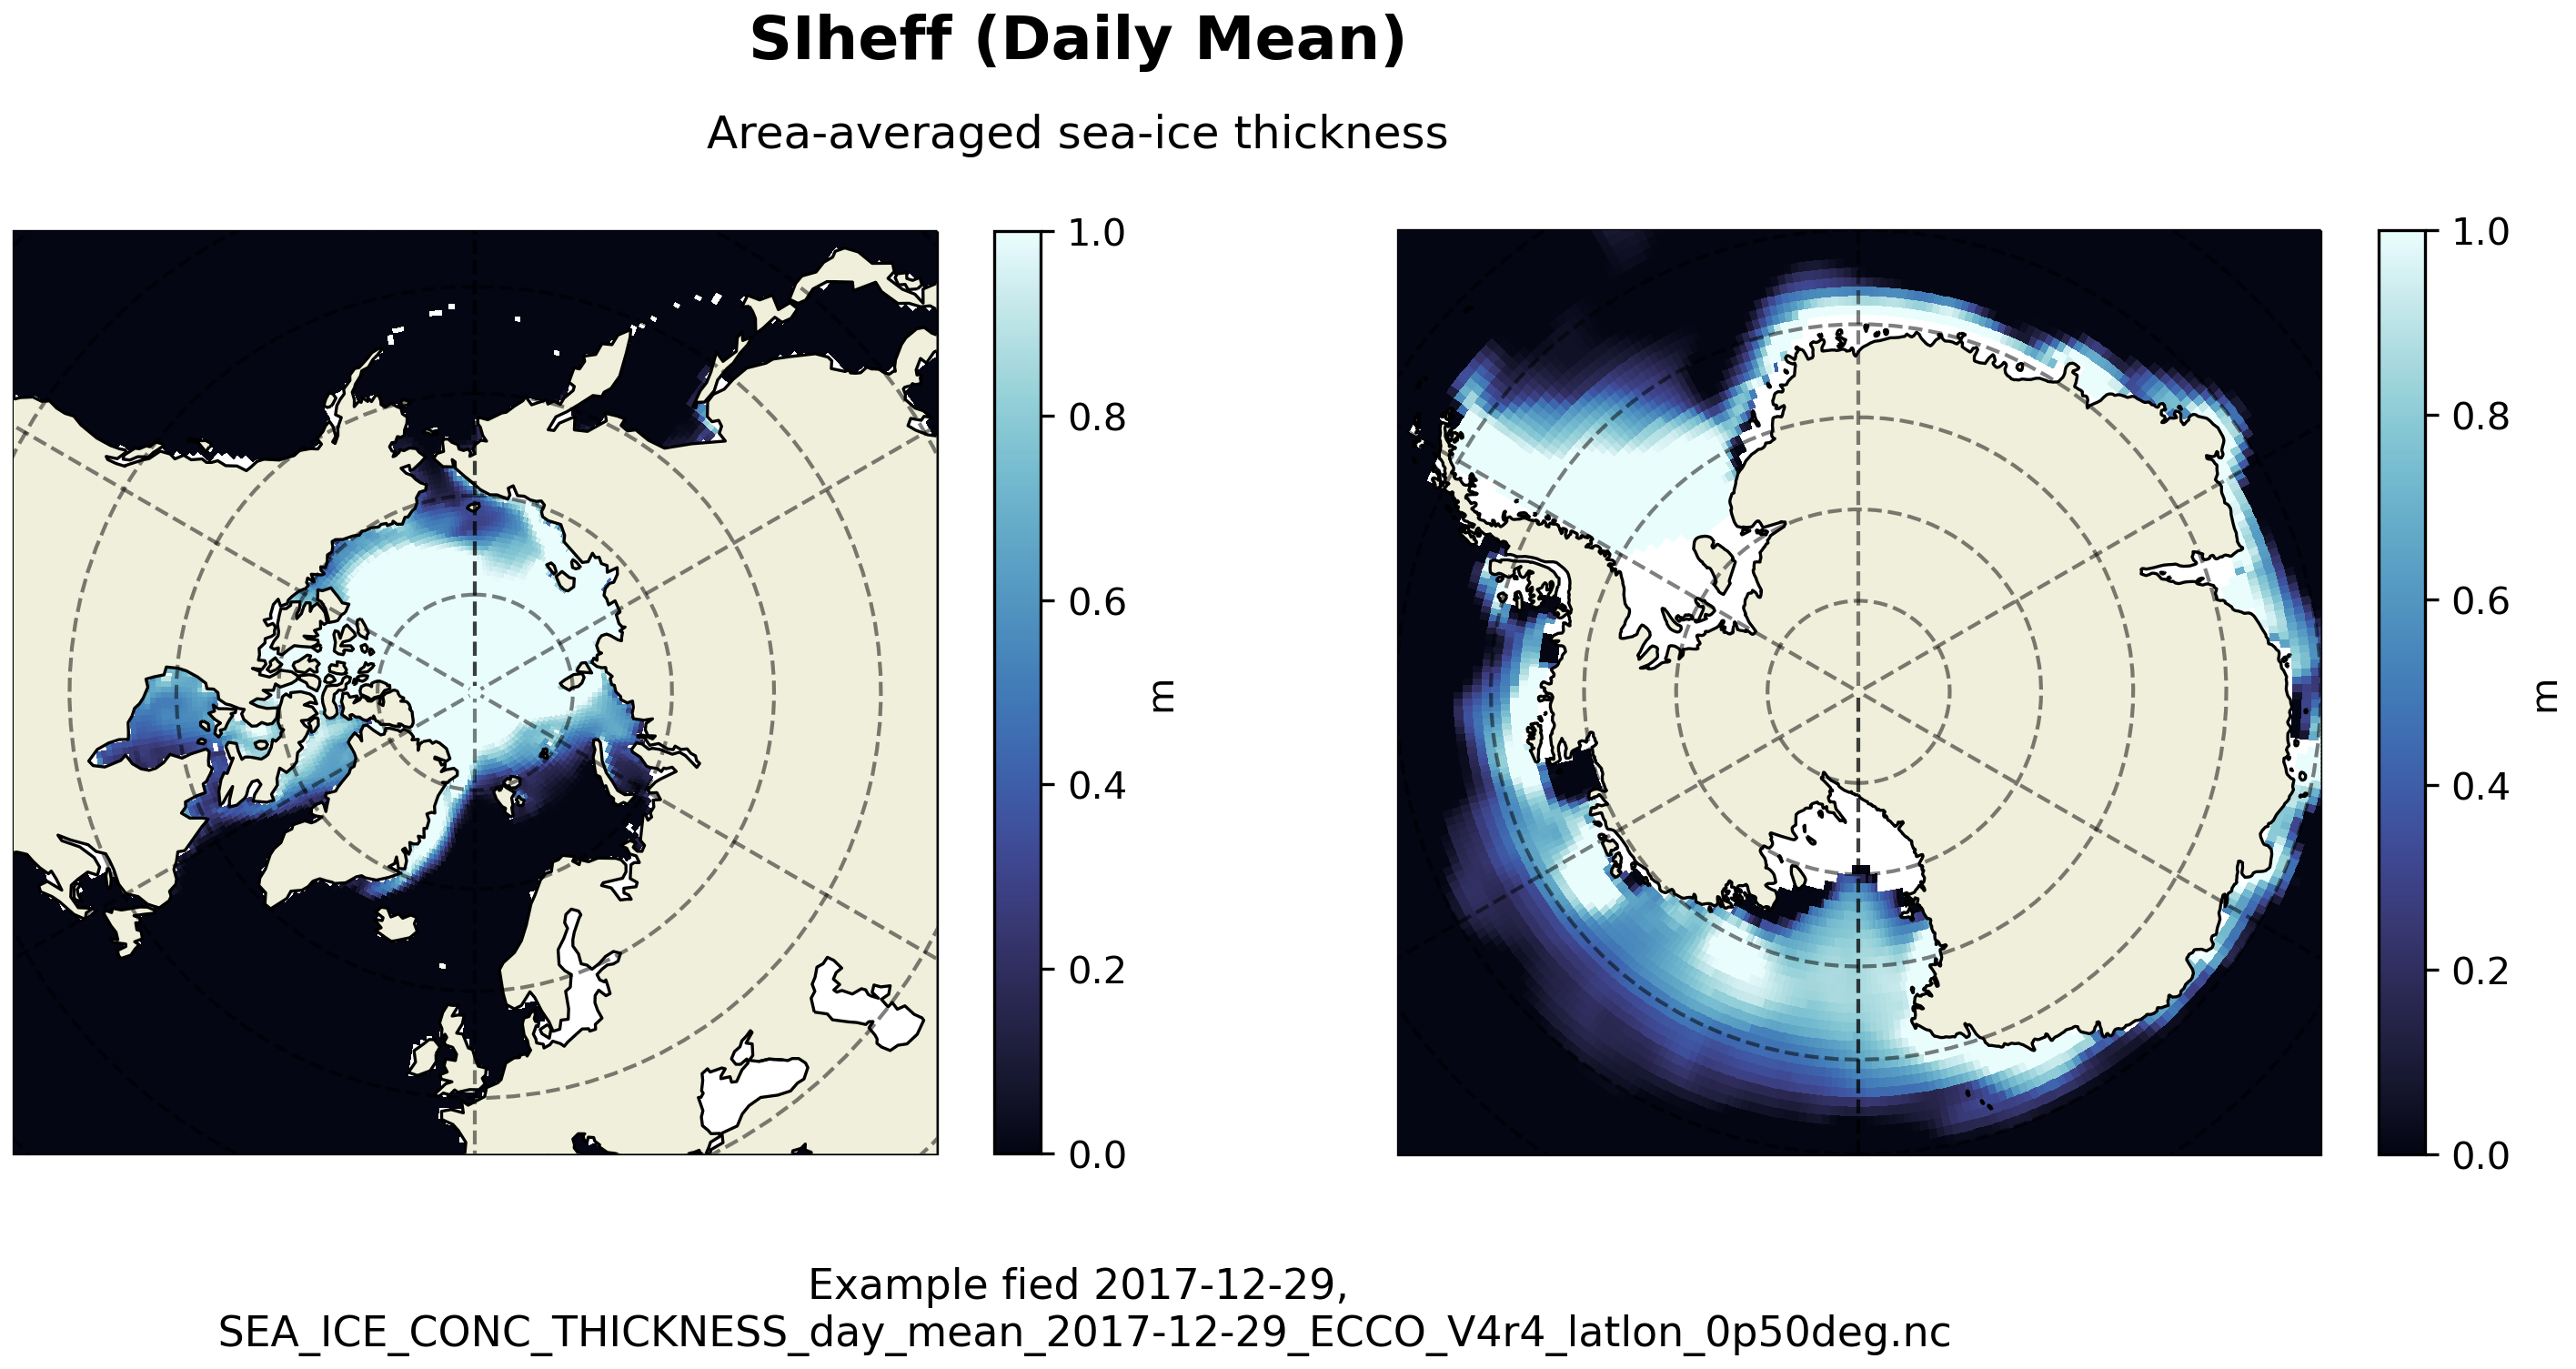
\includegraphics[width=\textwidth]{../images/plots/latlon_plots/Sea-Ice_and_Snow_Concentration_and_Thickness/SIheff.png}
\caption{Dataset: SEA\_ICE\_CONC\_THICKNESS Variable: SIheff}
\label{tab:table-SEA_ICE_CONC_THICKNESS_SIheff-Plot}
\end{figure}
\pagebreak
\subsubsection{Latlon Variable SIhsnow}
\begin{longtable}{|p{0.06\textwidth}|p{0.41\textwidth}|p{0.39\textwidth}|p{0.06\textwidth}|}
\caption{CDL description of SEA\_ICE\_CONC\_THICKNESS's SIhsnow variable}
\label{tab:table-SEA_ICE_CONC_THICKNESS_SIhsnow} \\ 
\hline \endhead \hline \endfoot
\rowcolor{lightgray} \textbf{Storage Type} & \textbf{Variable Name} & \textbf{Description} & \textbf{Unit} \\ \hline
float32 & SIhsnow & Area-averaged snow thickness & m \\ \hline
\rowcolor{lightgray}  \multicolumn{4}{|p{1.00\textwidth}|}{\textbf{CDL Description}} \\ \hline
\multicolumn{4}{|p{1.00\textwidth}|}{\makecell{\parbox{1\textwidth}{float32 SIhsnow(time, latitude, longitude)\\
\hspace*{0.5cm}SIhsnow: \_FillValue = 9.96921e+36\\
\hspace*{0.5cm}SIhsnow: coverage\_content\_type = modelResult\\
\hspace*{0.5cm}SIhsnow: long\_name = Area: averaged snow thickness\\
\hspace*{0.5cm}SIhsnow: standard\_name = surface\_snow\_thickness\\
\hspace*{0.5cm}SIhsnow: units = m\\
\hspace*{0.5cm}SIhsnow: coordinates = time\\
\hspace*{0.5cm}SIhsnow: valid\_min = : 0.0004725505714304745\\
\hspace*{0.5cm}SIhsnow: valid\_max = 2.5671639442443848}}} \\ \hline
\rowcolor{lightgray} \multicolumn{4}{|p{1.00\textwidth}|}{\textbf{Comments}} \\ \hline
\multicolumn{4}{|p{1\textwidth}|}{Snow thickness averaged over the entire model grid cell, including open water where snow thickness is zero. Note: snow thickness over the ICE-COVERED fraction of the grid cell is SIhsnow/SIarea} \\ \hline
\end{longtable}

\begin{figure}[H]
\centering
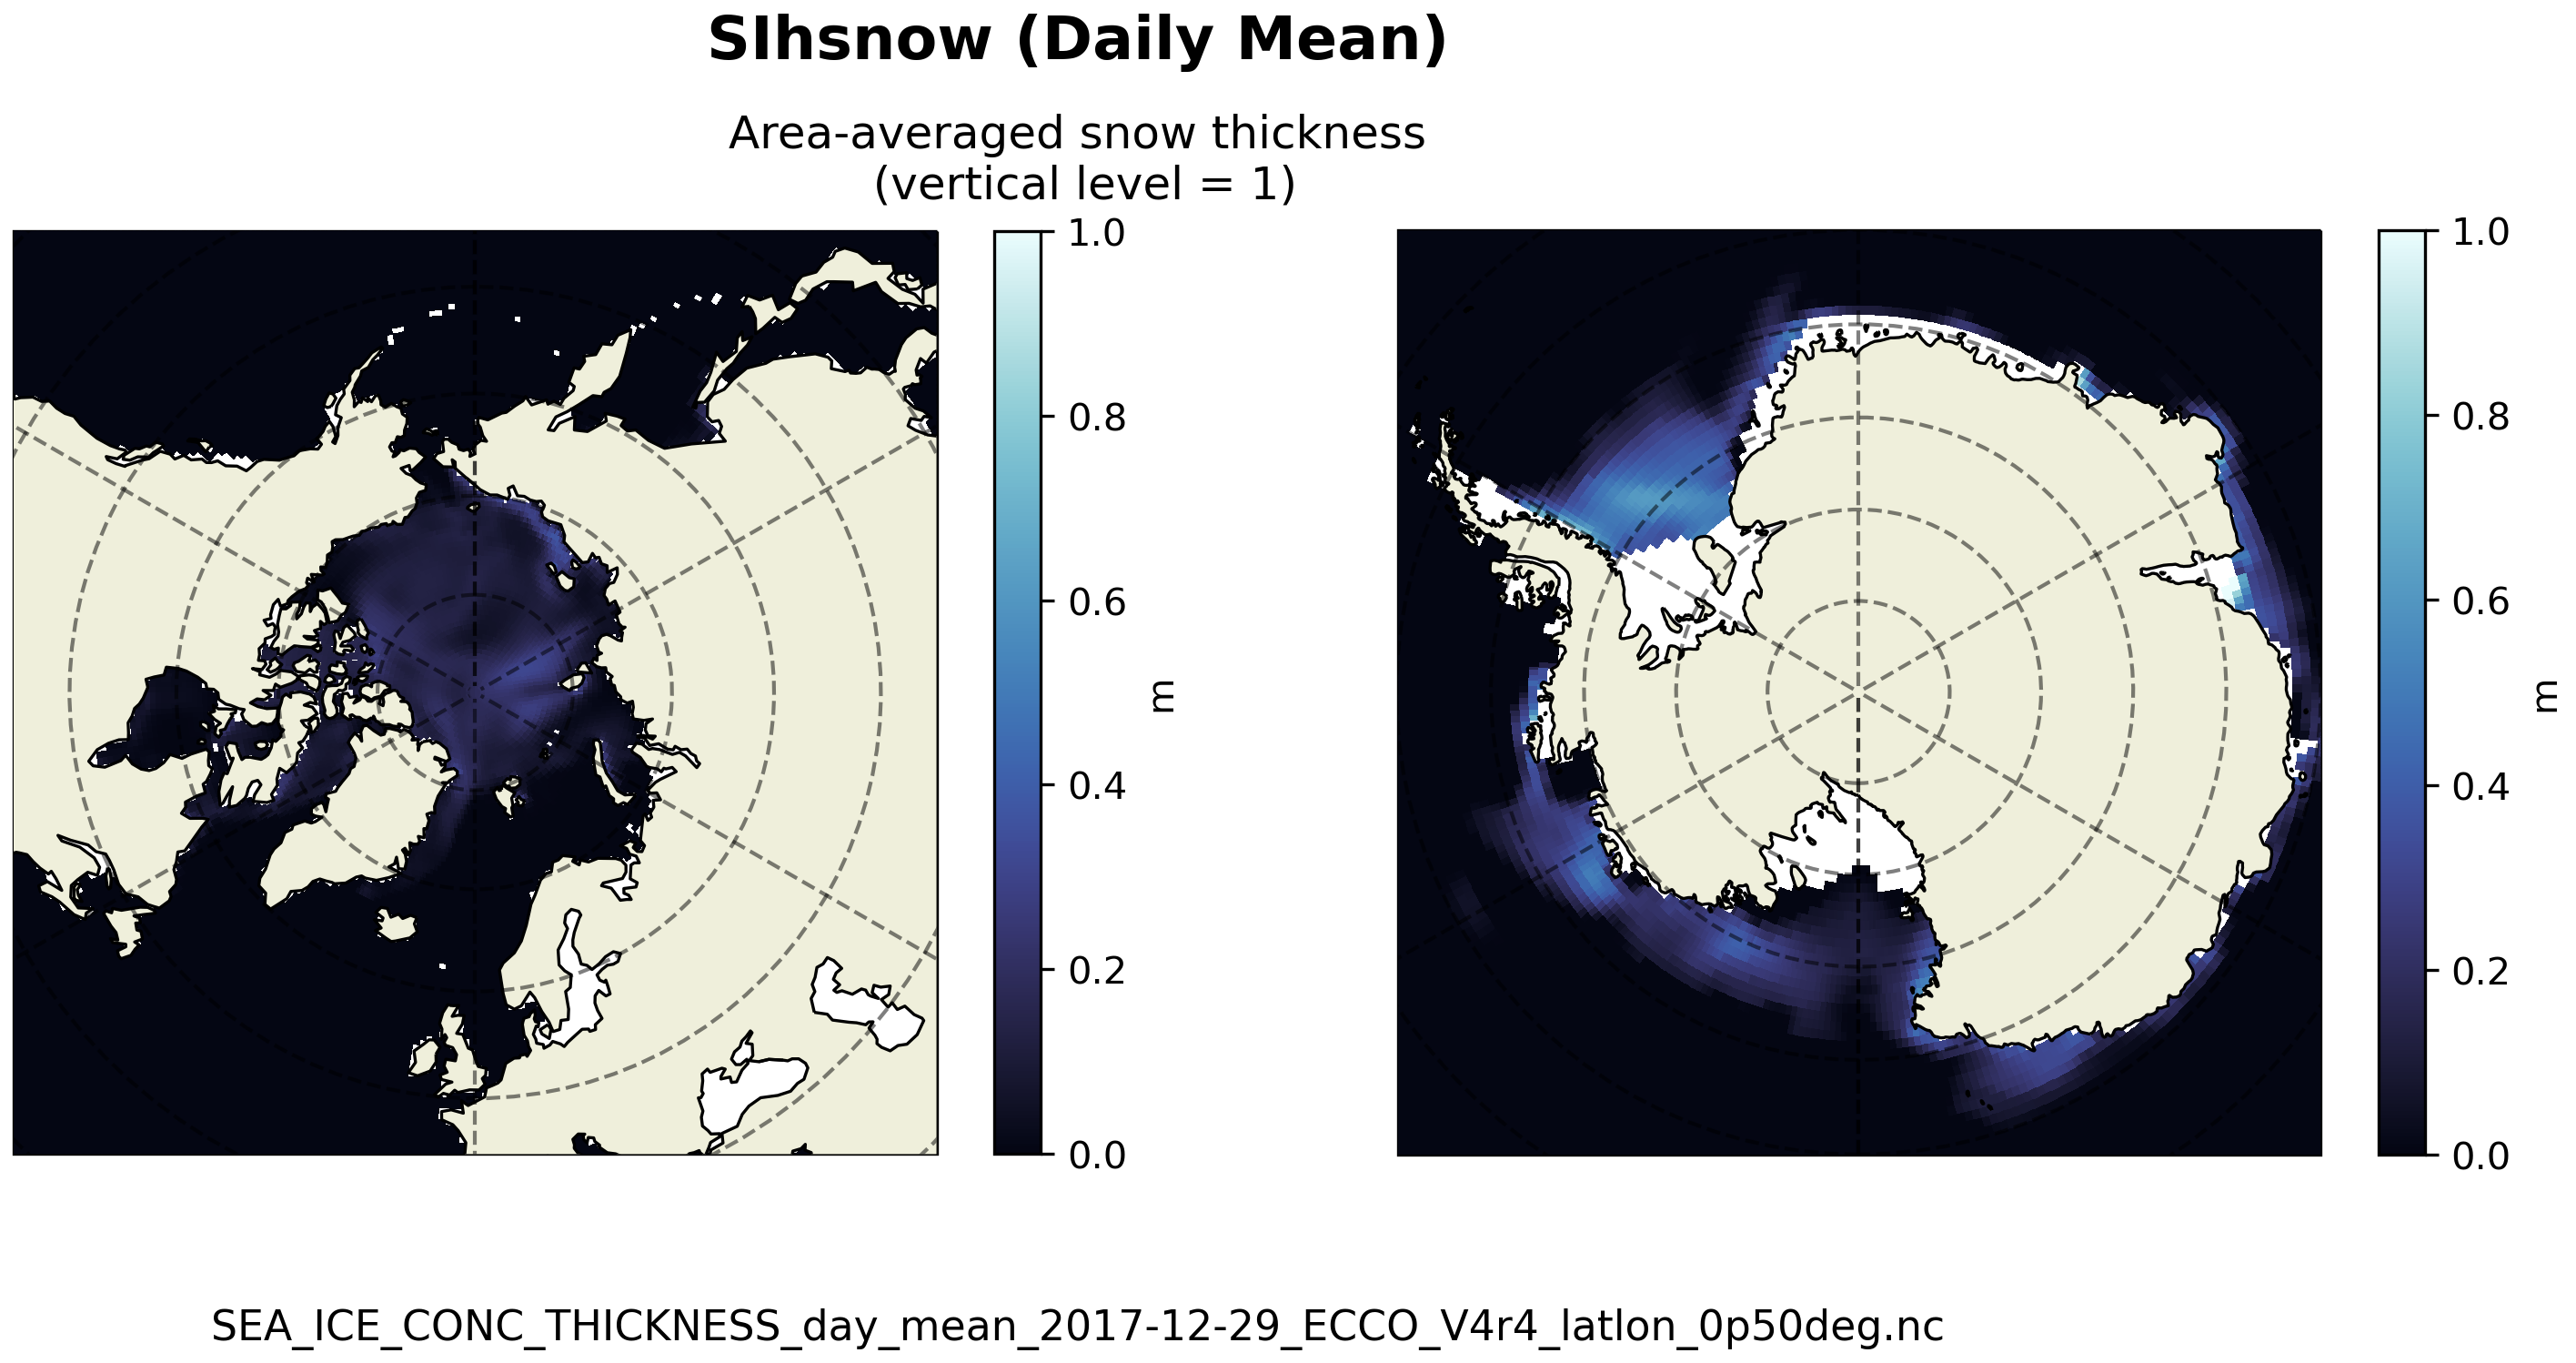
\includegraphics[width=\textwidth]{../images/plots/latlon_plots/Sea-Ice_and_Snow_Concentration_and_Thickness/SIhsnow.png}
\caption{Dataset: SEA\_ICE\_CONC\_THICKNESS Variable: SIhsnow}
\label{tab:table-SEA_ICE_CONC_THICKNESS_SIhsnow-Plot}
\end{figure}
\pagebreak
\subsubsection{Latlon Variable sIceLoad}
\begin{longtable}{|p{0.06\textwidth}|p{0.41\textwidth}|p{0.39\textwidth}|p{0.06\textwidth}|}
\caption{CDL description of SEA\_ICE\_CONC\_THICKNESS's sIceLoad variable}
\label{tab:table-SEA_ICE_CONC_THICKNESS_sIceLoad} \\ 
\hline \endhead \hline \endfoot
\rowcolor{lightgray} \textbf{Storage Type} & \textbf{Variable Name} & \textbf{Description} & \textbf{Unit} \\ \hline
float32 & sIceLoad & Average sea-ice and snow mass per unit area & kg m-2 \\ \hline
\rowcolor{lightgray}  \multicolumn{4}{|p{1.00\textwidth}|}{\textbf{CDL Description}} \\ \hline
\multicolumn{4}{|p{1.00\textwidth}|}{\makecell{\parbox{1\textwidth}{float32 sIceLoad(time, latitude, longitude)\\
\hspace*{0.5cm}sIceLoad: \_FillValue = 9.96921e+36\\
\hspace*{0.5cm}sIceLoad: coverage\_content\_type = modelResult\\
\hspace*{0.5cm}sIceLoad: long\_name = Average sea: ice and snow mass per unit area\\
\hspace*{0.5cm}sIceLoad: standard\_name = sea\_ice\_and\_surface\_snow\_amount\\
\hspace*{0.5cm}sIceLoad: units = kg m: 2\\
\hspace*{0.5cm}sIceLoad: coordinates = time\\
\hspace*{0.5cm}sIceLoad: valid\_min = : 0.0015558383893221617\\
\hspace*{0.5cm}sIceLoad: valid\_max = 8729.935546875}}} \\ \hline
\rowcolor{lightgray} \multicolumn{4}{|p{1.00\textwidth}|}{\textbf{Comments}} \\ \hline
\multicolumn{4}{|p{1\textwidth}|}{Total mass of sea-ice and snow in a model grid cell averaged over model grid cell area. Note: sIceLoad is used to correct model sea level anomaly, ETAN, to calculate dynamic sea surface height, SSH, and sea surface height without the inverted barometer (IB correction), SSHNOIBC. In the model, sea-ice is treated as floating above the sea level with ETAN tracing the location of the ocean-ice interface. Consequently, sea-ice growth in the model lowers ETAN and sea-ice melting raises ETAN. Dynamic sea surface height is obtained by correcting ETAN by the weight of ice and snow directly above following Archimedes’ principle.} \\ \hline
\end{longtable}

\begin{figure}[H]
\centering
\includegraphics[width=\textwidth]{../images/plots/latlon_plots/Sea-Ice_and_Snow_Concentration_and_Thickness/sIceLoad.png}
\caption{Dataset: SEA\_ICE\_CONC\_THICKNESS Variable: sIceLoad}
\label{tab:table-SEA_ICE_CONC_THICKNESS_sIceLoad-Plot}
\end{figure}
\pagebreak
\subsection{Latlon NetCDF SEA\_ICE\_VELOCITY}
\newp
\begin{longtable}{|p{0.1\textwidth}|p{0.5\textwidth}|}
\caption{Variables in the dataset SEA\_ICE\_VELOCITY}
\label{tab:table-SEA_ICE_VELOCITY-fields} \\ 
\hline \endhead \hline \endfoot
\rowcolor{lightgray} \textbf{Dataset:} & \textbf{SEA\_ICE\_VELOCITY} \\ \hline
Field: &SIeice \\ \hline
Field: &SInice \\ \hline
\end{longtable}

\pagebreak
\subsubsection{Latlon Variable SIeice}
\begin{longtable}{|p{0.06\textwidth}|p{0.41\textwidth}|p{0.39\textwidth}|p{0.06\textwidth}|}
\caption{CDL description of SEA\_ICE\_VELOCITY's SIeice variable}
\label{tab:table-SEA_ICE_VELOCITY_SIeice} \\ 
\hline \endhead \hline \endfoot
\rowcolor{lightgray} \textbf{Storage Type} & \textbf{Variable Name} & \textbf{Description} & \textbf{Unit} \\ \hline
float32 & SIeice & Zonal (east-west) sea-ice velocity & m s-1 \\ \hline
\rowcolor{lightgray}  \multicolumn{4}{|p{1.00\textwidth}|}{\textbf{CDL Description}} \\ \hline
\multicolumn{4}{|p{1.00\textwidth}|}{\makecell{\parbox{1\textwidth}{float32 SIeice(time, latitude, longitude)\\
\hspace*{0.5cm}SIeice: \_FillValue = 9.96921e+36\\
\hspace*{0.5cm}SIeice: coverage\_content\_type = modelResult\\
\hspace*{0.5cm}SIeice: long\_name = Zonal (east: west) sea: ice velocity\\
\hspace*{0.5cm}SIeice: standard\_name = eastward\_sea\_ice\_velocity\\
\hspace*{0.5cm}SIeice: units = m s: 1\\
\hspace*{0.5cm}SIeice: coordinates = time\\
\hspace*{0.5cm}SIeice: valid\_min = : 0.5656854510307312\\
\hspace*{0.5cm}SIeice: valid\_max = 0.5656854510307312}}} \\ \hline
\rowcolor{lightgray} \multicolumn{4}{|p{1.00\textwidth}|}{\textbf{Comments}} \\ \hline
\multicolumn{4}{|p{1\textwidth}|}{Zonal (east-west) componet of sea-ice velocity. Note: mask with SIarea to remove nonzero values where ice is absent. SIeice is calculated by interpolating the model's x and y components of sea-ice velocity (SIuice and SIvice) to tracer cell centers and then finding the zonal component of the interpolated vectors. It is NOT recommended to use SIuice and SIvice for sea-ice volume budget calculations because interpolating SIuice and SIvice from the model grid to the lat-lon grid introduces errors. Perform sea-ice mass budget calculations with ADVxHEFF, ADVyHEFF, DFxHEFF, and DFyHEFF on the native model grid.} \\ \hline
\end{longtable}

\begin{figure}[H]
\centering
\includegraphics[width=\textwidth]{../images/plots/latlon_plots/Sea-Ice_Velocity/SIeice.png}
\caption{Dataset: SEA\_ICE\_VELOCITY Variable: SIeice}
\label{tab:table-SEA_ICE_VELOCITY_SIeice-Plot}
\end{figure}
\pagebreak
\subsubsection{Latlon Variable SInice}
\begin{longtable}{|p{0.06\textwidth}|p{0.41\textwidth}|p{0.39\textwidth}|p{0.06\textwidth}|}
\caption{CDL description of SEA\_ICE\_VELOCITY's SInice variable}
\label{tab:table-SEA_ICE_VELOCITY_SInice} \\ 
\hline \endhead \hline \endfoot
\rowcolor{lightgray} \textbf{Storage Type} & \textbf{Variable Name} & \textbf{Description} & \textbf{Unit} \\ \hline
float32 & SInice & Meridional (north-south) sea-ice velocity & m s-1 \\ \hline
\rowcolor{lightgray}  \multicolumn{4}{|p{1.00\textwidth}|}{\textbf{CDL Description}} \\ \hline
\multicolumn{4}{|p{1.00\textwidth}|}{\makecell{\parbox{1\textwidth}{float32 SInice(time, latitude, longitude)\\
\hspace*{0.5cm}SInice: \_FillValue = 9.96921e+36\\
\hspace*{0.5cm}SInice: coverage\_content\_type = modelResult\\
\hspace*{0.5cm}SInice: long\_name = Meridional (north: south) sea: ice velocity\\
\hspace*{0.5cm}SInice: standard\_name = northward\_sea\_ice\_velocity\\
\hspace*{0.5cm}SInice: units = m s: 1\\
\hspace*{0.5cm}SInice: coordinates = time\\
\hspace*{0.5cm}SInice: valid\_min = : 0.5615208148956299\\
\hspace*{0.5cm}SInice: valid\_max = 0.5656854510307312}}} \\ \hline
\rowcolor{lightgray} \multicolumn{4}{|p{1.00\textwidth}|}{\textbf{Comments}} \\ \hline
\multicolumn{4}{|p{1\textwidth}|}{Meridional (north-south) component of sea-ice velocity. Note: mask with SIarea to remove nonzero values where ice is absent. SInice is calculated by interpolating the model's x and y components of sea-ice velocity (SIuice and SIvice) to tracer cell centers and then finding the meridional component of the interpolated vectors. It is NOT recommended to use SIuice and SIvice for sea-ice volume budget calculations because interpolating SIuice and SIvice from the model grid to the lat-lon grid introduces errors. Perform sea-ice mass budget calculations with ADVxHEFF, ADVyHEFF, DFxHEFF, and DFyHEFF on the native model grid.} \\ \hline
\end{longtable}

\begin{figure}[H]
\centering
\includegraphics[width=\textwidth]{../images/plots/latlon_plots/Sea-Ice_Velocity/SInice.png}
\caption{Dataset: SEA\_ICE\_VELOCITY Variable: SInice}
\label{tab:table-SEA_ICE_VELOCITY_SInice-Plot}
\end{figure}
\pagebreak
\subsection{Latlon NetCDF SEA\_SURFACE\_HEIGHT}
\newp
\begin{longtable}{|p{0.1\textwidth}|p{0.5\textwidth}|}
\caption{Variables in the dataset SEA\_SURFACE\_HEIGHT}
\label{tab:table-SEA_SURFACE_HEIGHT-fields} \\ 
\hline \endhead \hline \endfoot
\rowcolor{lightgray} \textbf{Dataset:} & \textbf{SEA\_SURFACE\_HEIGHT} \\ \hline
Field: &SSH \\ \hline
Field: &SSHIBC \\ \hline
Field: &SSHNOIBC \\ \hline
\end{longtable}

\pagebreak
\subsubsection{Latlon Variable SSH}
\begin{longtable}{|p{0.06\textwidth}|p{0.41\textwidth}|p{0.39\textwidth}|p{0.06\textwidth}|}
\caption{CDL description of SEA\_SURFACE\_HEIGHT's SSH variable}
\label{tab:table-SEA_SURFACE_HEIGHT_SSH} \\ 
\hline \endhead \hline \endfoot
\rowcolor{lightgray} \textbf{Storage Type} & \textbf{Variable Name} & \textbf{Description} & \textbf{Unit} \\ \hline
float32 & SSH & Dynamic sea surface height anomaly & m \\ \hline
\rowcolor{lightgray}  \multicolumn{4}{|p{1.00\textwidth}|}{\textbf{CDL Description}} \\ \hline
\multicolumn{4}{|p{1.00\textwidth}|}{\makecell{\parbox{1\textwidth}{float32 SSH(time, latitude, longitude)\\
\hspace*{0.5cm}SSH: \_FillValue = 9.96921e+36\\
\hspace*{0.5cm}SSH: coverage\_content\_type = modelResult\\
\hspace*{0.5cm}SSH: long\_name = Dynamic sea surface height anomaly\\
\hspace*{0.5cm}SSH: standard\_name = sea\_surface\_height\_above\_geoid\\
\hspace*{0.5cm}SSH: units = m\\
\hspace*{0.5cm}SSH: coordinates = time\\
\hspace*{0.5cm}SSH: valid\_min = : 2.4861555099487305\\
\hspace*{0.5cm}SSH: valid\_max = 2.2875382900238037}}} \\ \hline
\rowcolor{lightgray} \multicolumn{4}{|p{1.00\textwidth}|}{\textbf{Comments}} \\ \hline
\multicolumn{4}{|p{1\textwidth}|}{Dynamic sea surface height anomaly above the geoid, suitable for comparisons with altimetry sea surface height data products that apply the inverse barometer (IB) correction. Note: SSH is calculated by correcting model sea level anomaly ETAN for three effects: a) global mean steric sea level changes related to density changes in the Boussinesq volume-conserving model (Greatbatch correction, see sterGloH), b) the inverted barometer (IB) effect (see SSHIBC) and c) sea level displacement due to sea-ice and snow pressure loading (see sIceLoad). SSH can be compared with the similarly-named SSH variable in previous ECCO products that did not include atmospheric pressure loading (e.g., Version 4 Release 3). Use SSHNOIBC for comparisons with altimetry data products that do NOT apply the IB correction.} \\ \hline
\end{longtable}

\begin{figure}[H]
\centering
\includegraphics[width=\textwidth]{../images/plots/latlon_plots/Sea_Surface_Height/SSH.png}
\caption{Dataset: SEA\_SURFACE\_HEIGHT Variable: SSH}
\label{tab:table-SEA_SURFACE_HEIGHT_SSH-Plot}
\end{figure}
\pagebreak
\subsubsection{Latlon Variable SSHIBC}
\begin{longtable}{|p{0.06\textwidth}|p{0.41\textwidth}|p{0.39\textwidth}|p{0.06\textwidth}|}
\caption{CDL description of SEA\_SURFACE\_HEIGHT's SSHIBC variable}
\label{tab:table-SEA_SURFACE_HEIGHT_SSHIBC} \\ 
\hline \endhead \hline \endfoot
\rowcolor{lightgray} \textbf{Storage Type} & \textbf{Variable Name} & \textbf{Description} & \textbf{Unit} \\ \hline
float32 & SSHIBC & The inverted barometer (IB) correction to sea surface height due to atmospheric pressure loading & m \\ \hline
\rowcolor{lightgray}  \multicolumn{4}{|p{1.00\textwidth}|}{\textbf{CDL Description}} \\ \hline
\multicolumn{4}{|p{1.00\textwidth}|}{\makecell{\parbox{1\textwidth}{float32 SSHIBC(time, latitude, longitude)\\
\hspace*{0.5cm}SSHIBC: \_FillValue = 9.96921e+36\\
\hspace*{0.5cm}SSHIBC: coverage\_content\_type = modelResult\\
\hspace*{0.5cm}SSHIBC: long\_name = The inverted barometer (IB) correction to sea surface height due to atmospheric pressure loading\\
\hspace*{0.5cm}SSHIBC: units = m\\
\hspace*{0.5cm}SSHIBC: coordinates = time\\
\hspace*{0.5cm}SSHIBC: valid\_min = : 0.5228679180145264\\
\hspace*{0.5cm}SSHIBC: valid\_max = 0.8955588340759277}}} \\ \hline
\rowcolor{lightgray} \multicolumn{4}{|p{1.00\textwidth}|}{\textbf{Comments}} \\ \hline
\multicolumn{4}{|p{1\textwidth}|}{Not an SSH itself, but a correction to model sea level anomaly (ETAN) required to account for the static part of sea surface displacement by atmosphere pressure loading: SSH = SSHNOIBC - SSHIBC. Note: Use SSH for model-data comparisons with altimetry data products that DO apply the IB correction and SSHNOIBC for comparisons with altimetry data products that do NOT apply the IB correction.} \\ \hline
\end{longtable}

\begin{figure}[H]
\centering
\includegraphics[width=\textwidth]{../images/plots/latlon_plots/Sea_Surface_Height/SSHIBC.png}
\caption{Dataset: SEA\_SURFACE\_HEIGHT Variable: SSHIBC}
\label{tab:table-SEA_SURFACE_HEIGHT_SSHIBC-Plot}
\end{figure}
\pagebreak
\subsubsection{Latlon Variable SSHNOIBC}
\begin{longtable}{|p{0.06\textwidth}|p{0.41\textwidth}|p{0.39\textwidth}|p{0.06\textwidth}|}
\caption{CDL description of SEA\_SURFACE\_HEIGHT's SSHNOIBC variable}
\label{tab:table-SEA_SURFACE_HEIGHT_SSHNOIBC} \\ 
\hline \endhead \hline \endfoot
\rowcolor{lightgray} \textbf{Storage Type} & \textbf{Variable Name} & \textbf{Description} & \textbf{Unit} \\ \hline
float32 & SSHNOIBC & Sea surface height anomaly without the inverted barometer (IB) correction & m \\ \hline
\rowcolor{lightgray}  \multicolumn{4}{|p{1.00\textwidth}|}{\textbf{CDL Description}} \\ \hline
\multicolumn{4}{|p{1.00\textwidth}|}{\makecell{\parbox{1\textwidth}{float32 SSHNOIBC(time, latitude, longitude)\\
\hspace*{0.5cm}SSHNOIBC: \_FillValue = 9.96921e+36\\
\hspace*{0.5cm}SSHNOIBC: coverage\_content\_type = modelResult\\
\hspace*{0.5cm}SSHNOIBC: long\_name = Sea surface height anomaly without the inverted barometer (IB) correction\\
\hspace*{0.5cm}SSHNOIBC: units = m\\
\hspace*{0.5cm}SSHNOIBC: coordinates = time\\
\hspace*{0.5cm}SSHNOIBC: valid\_min = : 2.45104718208313\\
\hspace*{0.5cm}SSHNOIBC: valid\_max = 2.2390522956848145}}} \\ \hline
\rowcolor{lightgray} \multicolumn{4}{|p{1.00\textwidth}|}{\textbf{Comments}} \\ \hline
\multicolumn{4}{|p{1\textwidth}|}{Sea surface height anomaly above the geoid without the inverse barometer (IB) correction, suitable for comparisons with altimetry sea surface height data products that do NOT apply the inverse barometer (IB) correction. Note: SSHNOIBC is calculated by correcting model sea level anomaly ETAN for two effects: a) global mean steric sea level changes related to density changes in the Boussinesq volume-conserving model (Greatbatch correction, see sterGloH), b) sea level displacement due to sea-ice and snow pressure loading (see sIceLoad). In ECCO Version 4 Release 4 the model is forced with atmospheric pressure loading. SSHNOIBC does not correct for the static part of the effect of atmosphere pressure loading on sea surface height (the so-called inverse barometer (IB) correction). Use SSH for comparisons with altimetry data products that DO apply the IB correction.} \\ \hline
\end{longtable}

\begin{figure}[H]
\centering
\includegraphics[width=\textwidth]{../images/plots/latlon_plots/Sea_Surface_Height/SSHNOIBC.png}
\caption{Dataset: SEA\_SURFACE\_HEIGHT Variable: SSHNOIBC}
\label{tab:table-SEA_SURFACE_HEIGHT_SSHNOIBC-Plot}
\end{figure}